%!TeX spellcheck = hu_HU
\documentclass[a4paper,12pt]{article}
% !TeX spellcheck = en_US

\usepackage[utf8x]{inputenc}
\usepackage[margin=1in,headheight=14.5pt]{geometry}
%\usepackage[top=1in,bottom=1in,right=0.7in,left=1.3in,headheight=14.5pt]{geometry}

\usepackage{fancyhdr}
\pagestyle{fancy}

\usepackage[english,romanian,hungarian]{babel}
\usepackage{indentfirst}

\usepackage[table,xcdraw,dvipsnames]{xcolor}
\definecolor{whitesmoke}{rgb}{0.96,0.96,0.96}
\definecolor{lightblue}{rgb}{0.22,0.45,0.70}
\definecolor{darkred}{rgb}{0.9,0.0,0.0}
\definecolor{darkpastelgreen}{rgb}{0.01,0.75,0.24}
\definecolor{flame}{rgb}{0.89,0.35,0.13}

\usepackage[unicode,pdfusetitle,backref=false,pagebackref=true]{hyperref}
%\hypersetup{colorlinks=true,urlcolor=lightblue,citecolor=darkpastelgreen,linkcolor=flame,pdfborder={0 0 0}}
\hypersetup{colorlinks=true,urlcolor=black,citecolor=black,linkcolor=black,pdfborder={0 0 0}}
\usepackage[all]{hypcap}
\usepackage{multirow}
\usepackage{letltxmacro}

\usepackage{graphicx}
\usepackage{wrapfig}
\usepackage{pdfpages}

\usepackage{booktabs}
\usepackage{multicol}
\usepackage{amsmath}

\usepackage[scale=1.25]{ccicons}

\usepackage{tikz}
\usetikzlibrary{arrows}
\tikzstyle{es} = [-triangle 60]

\usepackage{relsize}
\usepackage{enumitem}
\setlist[itemize]{itemsep=0pt}
\setlist[enumerate]{itemsep=0pt}

\setlength{\parskip}{0.25em}

\renewcommand{\arraystretch}{1.25}

\linespread{1.15}

\renewcommand{\UrlFont}{\ttfamily\relsize{-0.5}}

\usepackage[T1]{fontenc}
\usepackage{lmodern}
\usepackage{fontawesome}
\usepackage{inconsolata}

\usepackage{minted}
\renewcommand{\theFancyVerbLine}{\rmfamily\scriptsize\arabic{FancyVerbLine}}
\setminted{linenos,autogobble,breaklines,fontsize=\fontsize{10.5}{12.6},tabsize=4,numbersep=7pt,bgcolor=whitesmoke}
\AtBeginEnvironment{minted}{%
	\renewcommand{\fcolorbox}[4][]{#4}%
	\linespread{1.1}%
}

%
%	Override \cite and \ref to use bold face instead of a color.
%

\makeatletter
\def\@cite#1#2{[\textbf{#1\if@tempswa , #2\fi}]}
\makeatother

\AtBeginDocument{%
	\LetLtxMacro{\latexref}{\ref}%
	\def\ref#1{\textbf{\latexref{#1}}}%
}

%
%	Add "Retrieved from" and backlinks stylized by red arrows to the bibliography.
%

\newcommand{\urlprefix}{Retrieved from \urlstyle{rm}}

\newcommand{\refspace}{\vspace{-2mm}}
\newcommand{\redarrow}{\textbf{\textcolor{red}{$\mathbf{\to}$}}}

\makeatletter
\def\BR@@bibitem#1#2\par{
	\let\backrefprint\BR@backrefprint
	\def\@linkcolor{black}
	\BRorg@bibitem{#1}#2\redarrow \thinspace \BR@backref{#1}
}
\makeatother

%
%	Implement \subsubsubsection.
%

\usepackage{titlesec}

\titleclass{\subsubsubsection}{straight}[\subsection]

\newcounter{subsubsubsection}[subsubsection]
\renewcommand\thesubsubsubsection{\thesubsubsection.\arabic{subsubsubsection}}
\titleformat{\subsubsubsection}{\normalfont\normalsize\bfseries}{\thesubsubsubsection}{1em}{}
\titlespacing*{\subsubsubsection}{0pt}{3.25ex plus 1ex minus .2ex}{1.5ex plus .2ex}

\makeatletter
\def\toclevel@subsubsubsection{4}
\def\l@subsubsubsection{\@dottedtocline{4}{7em}{4em}}

\renewcommand\paragraph{\@startsection{paragraph}{6}{\parindent}{3.25ex \@plus1ex \@minus .2ex}{-1em}{\normalfont\normalsize\bfseries}}
\makeatother

\setcounter{secnumdepth}{4}
\setcounter{tocdepth}{4}

%
%	Implement Hungarian and Romanian section tracking for the English thesis.
%	\<lang>tableofcontents will print the corresponding one.
%

\makeatletter
\newcommand\hungariantableofcontents{
	\selectlanguage{hungarian}
	\section*{\contentsname
		\@mkboth{\MakeUppercase\contentsname}{\MakeUppercase\contentsname}}
	\@starttoc{2.toc}
	\selectlanguage{english}
}
\makeatother

\newcommand\sectionhu[1]{\addcontentsline{2.toc}{section} {\protect\numberline{\thesection} #1}}
\newcommand\subsectionhu[1]{\addcontentsline{2.toc}{subsection} {\protect\numberline{\thesubsection} #1}}
\newcommand\subsubsectionhu[1]{\addcontentsline{2.toc}{subsubsection} {\protect\numberline{\thesubsubsection} #1}}
\newcommand\subsubsubsectionhu[1]{\addcontentsline{2.toc}{subsubsubsection} {\protect\numberline{\thesubsubsubsection} #1}}

\makeatletter
\newcommand\romaniantableofcontents{
	\selectlanguage{romanian}
	\section*{\contentsname
		\@mkboth{\MakeUppercase\contentsname}{\MakeUppercase\contentsname}}
	\@starttoc{1.toc}
	\selectlanguage{english}
}
\makeatother

\newcommand\sectionro[1]{\addcontentsline{1.toc}{section} {\protect\numberline{\thesection} #1}}
\newcommand\subsectionro[1]{\addcontentsline{1.toc}{subsection} {\protect\numberline{\thesubsection} #1}}
\newcommand\subsubsectionro[1]{\addcontentsline{1.toc}{subsubsection} {\protect\numberline{\thesubsubsection} #1}}
\newcommand\subsubsubsectionro[1]{\addcontentsline{1.toc}{subsubsubsection} {\protect\numberline{\thesubsubsubsection} #1}}

%
%	Support for multiple \listof[figures|tables|listings] between parts of the document.
%	\clearcontents begins a new list.
%

\usepackage{xpatch}

\newcounter{lofcntr}
\newcounter{lotcntr}
\newcounter{lolcntr}

\NewDocumentCommand{\clearcontents}{}{
	\stepcounter{lofcntr}
	\stepcounter{lotcntr}
	\stepcounter{lolcntr}
	\setcounter{figure}{0}
	\setcounter{table}{0}
	\setcounter{listing}{0}
}

\makeatletter
\NewDocumentCommand{\advancecontents}{}{
	\def\ext@figure{\number\value{lofcntr}.\latex@ext@figure}
	\def\ext@table{\number\value{lotcntr}.\latex@ext@table}
	\@namedef{ext@listing}{\number\value{lolcntr}.\latex@ext@listing}
}

\AtBeginDocument{
	\let\latex@ext@figure\ext@figure
	\let\latex@ext@table\ext@table
	\let\latex@ext@listing\ext@listing
	\stepcounter{lofcntr}
	\stepcounter{lotcntr}
	\stepcounter{lolcntr}
	\advancecontents
}

\AtBeginDocument{
\xpretocmd{\caption}{
	\advancecontents
}{}{}
}

\xpatchcmd{\listoffigures}{%
	\@starttoc{lof}%
}{%
	\@starttoc{\number\value{lofcntr}.lof}%
}{}{}

\xpatchcmd{\listoftables}{%
	\@starttoc{lot}%
}{%
	\@starttoc{\number\value{lotcntr}.lot}%
}{}{}
\makeatother


\author{Gábor Zsolt }
\title{Thesis Computer Science Railway model automated}
\clearcontents

\begin{document}

% Ro Front
\newpage
\pagestyle{empty}
\selectlanguage{romanian}
    \begin{center}
        {\Large Universitatea Sapientia din Cluj-Napoca}\\\vspace{0.07in}
		{\Large Facultatea de Științe Tehnice și Umaniste, Târgu-Mureș}\\\vspace{0.07in}
		{\Large Specializarea Calculatoare}\\
		
		\vspace{2.35in}
		
		{\huge Digitalizare unui model electromecanic }\\\vspace{0.15in}
		{\huge feroviar, bazată pe principii ETCS}
		
		\vspace{0.5in}
		
		{\LARGE Proiect de Diplomă }
		
	\end{center}
	
	\vspace{2.0in}
	
	\begin{multicols}{2}
		\begin{flushleft}
			{\Large Coordonator științific:}
		\end{flushleft}
		\columnbreak
		\begin{flushright}
			{\Large Absolvent:}
		\end{flushright}
	\end{multicols}
	\begin{multicols}{2}
		\begin{flushleft}
			{\LARGE Dr. Székely Sándor Endre}
		\end{flushleft}
		\columnbreak
		\begin{flushright}
			{\LARGE Gábor Zsolt}
		\end{flushright}
	\end{multicols}
	
	\vspace{1.5in}
		
	\begin{center}
		{\LARGE 2019}
	\end{center}
	
\newpage
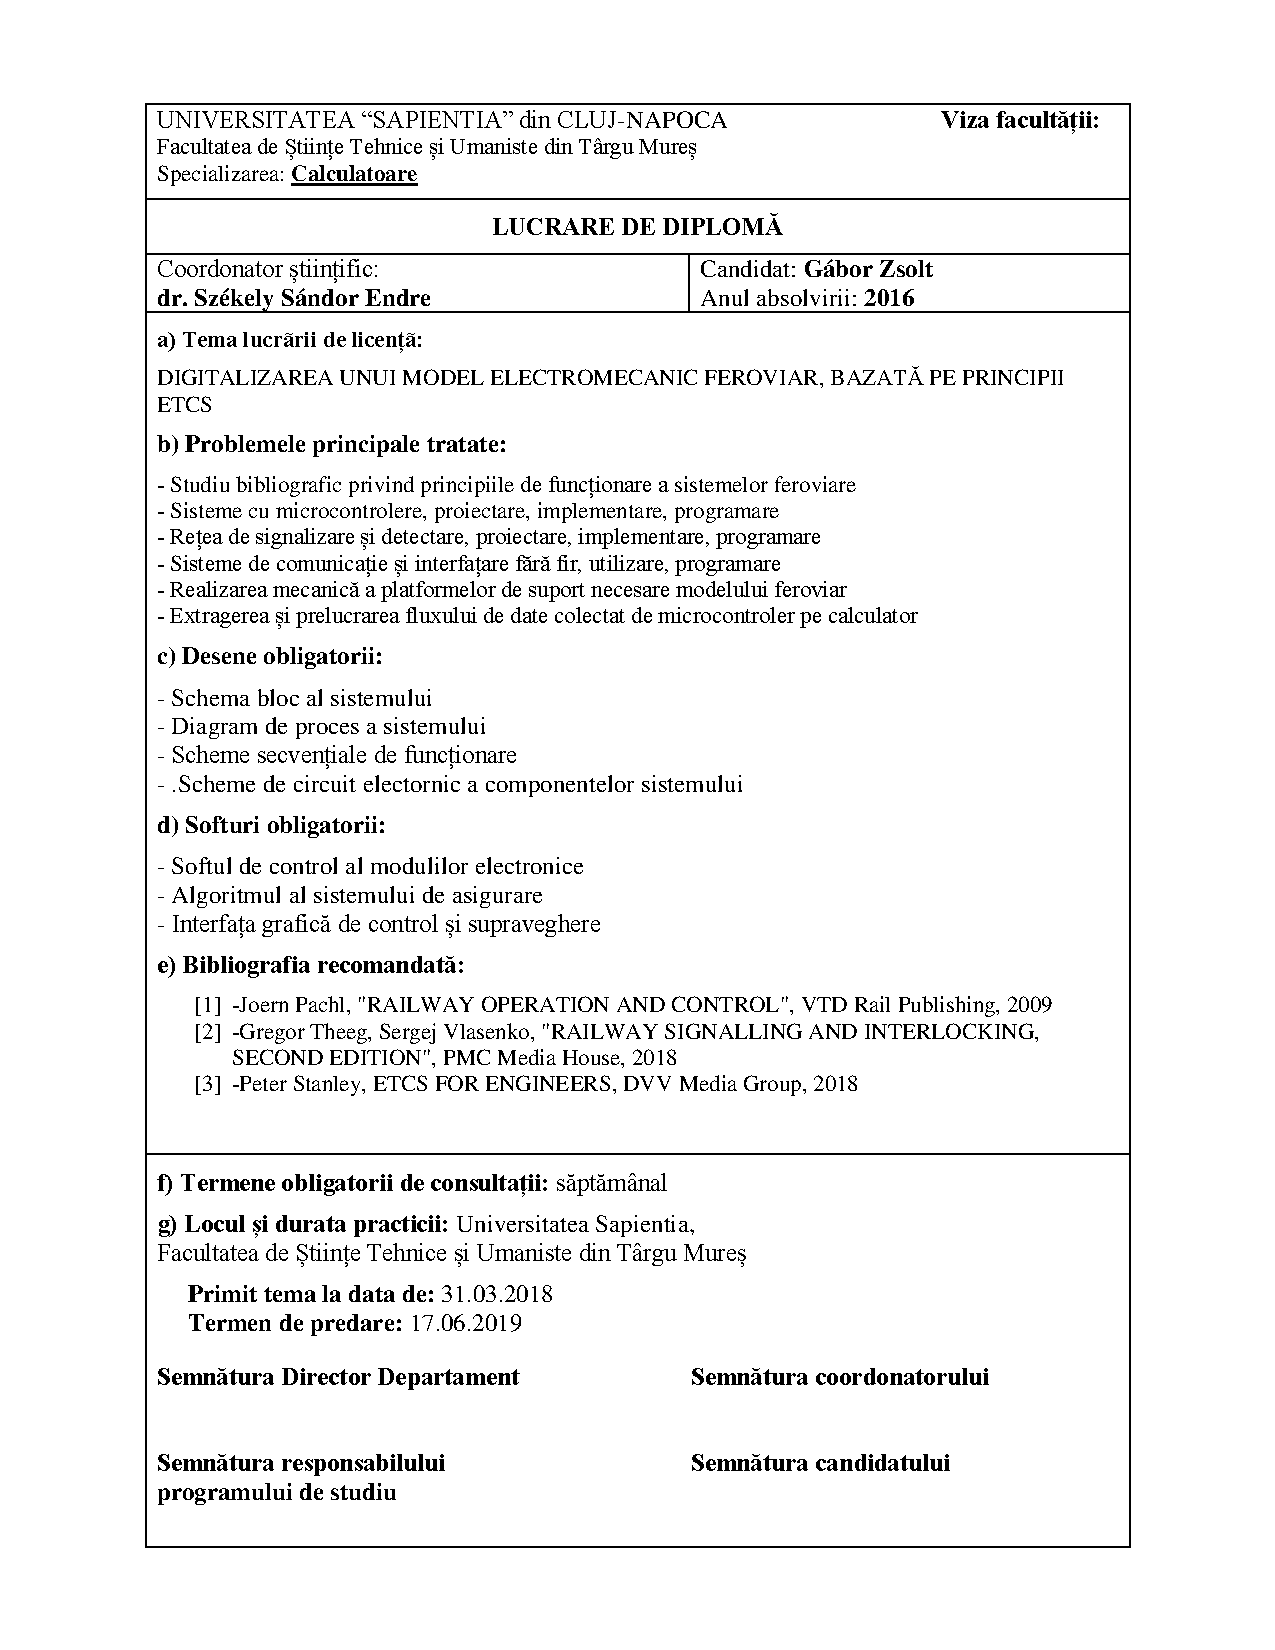
\includepdf[pages=-]{Detalii_licenta_RO.pdf} 
\newpage
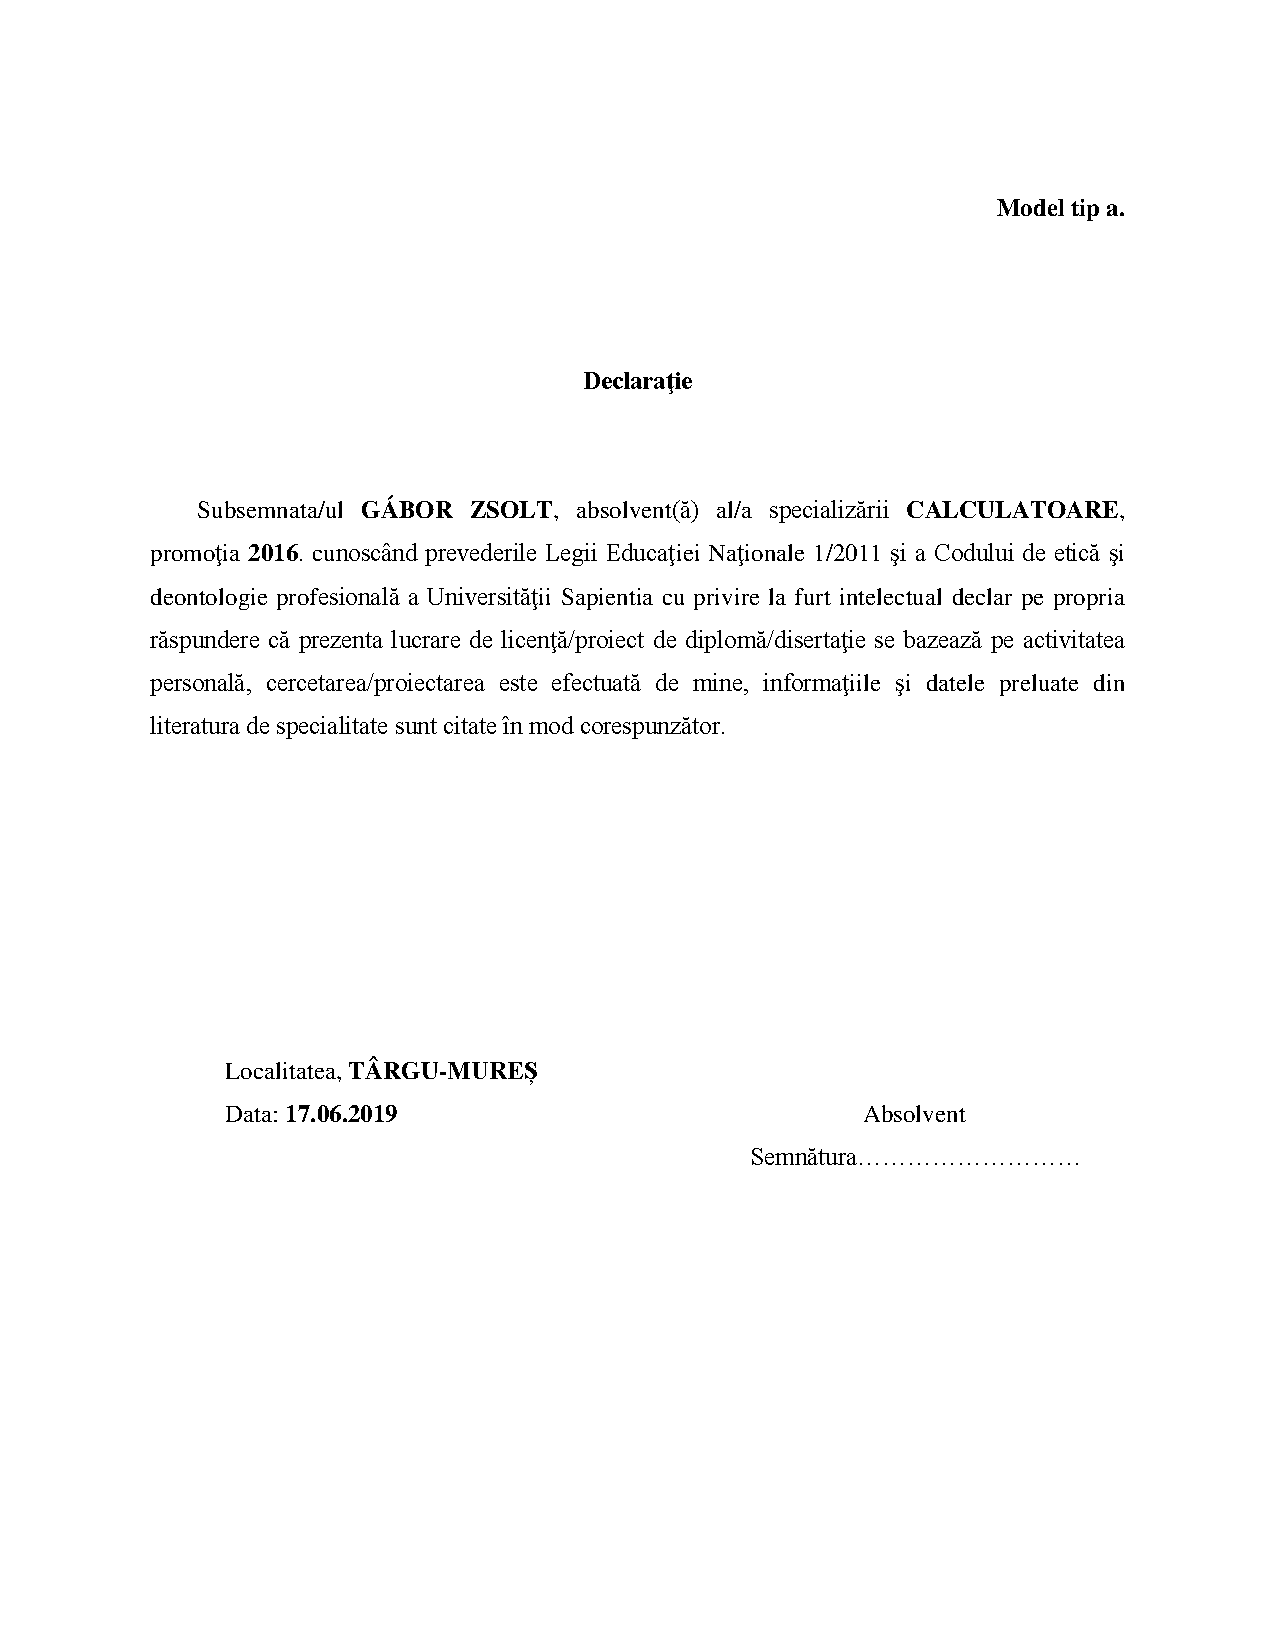
\includepdf[pages=-]{Declaratii_licenta_RO.pdf}
%Romanian abstract
\newpage
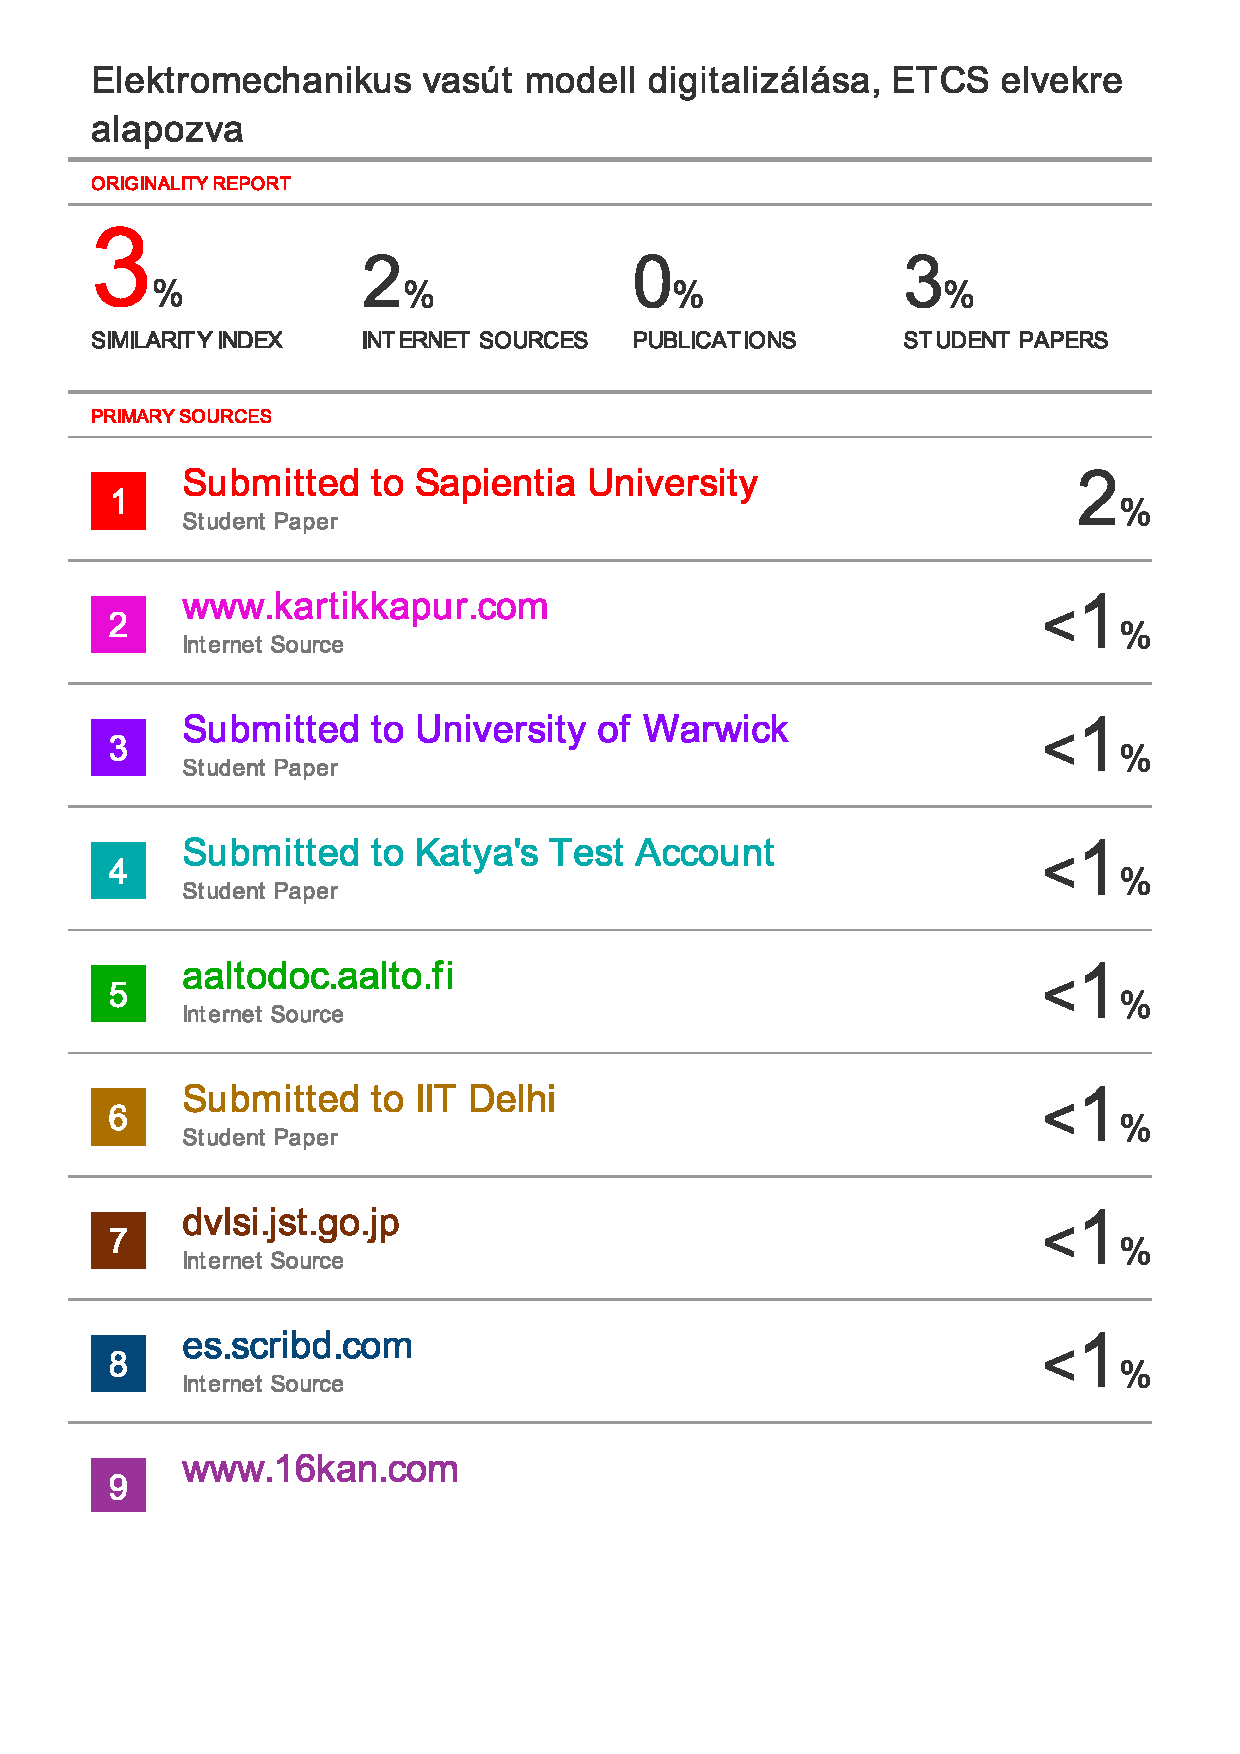
\includepdf[pages=-]{turnitin_report.pdf}

\newpage
\pagestyle{empty}
\begin{center}
		{\huge Digitalizare unui model electromecanic }\\\vspace{0.15in}
		{\huge feroviar, bazată pe principii ETCS}
	\vspace{0.1in}
	
    {\LARGE Extras}
\end{center}

Transportul feroviar în zilele noastre e o componentă organică al economiei și al transportului de masă.
Problema principală în tranzitul universal între diferite rețele ferate, este faptul că la nivel de țară sistemul de protecție al trenurilor diferă.
Pentru a soluționa această dificultate, prin UE, sa stabilit ERA (Agenția europeană de transport feroviar) care a dezvoltat sistemul universal ETCS.
Scopul lucrării mele de diplomă este de a integra aceste principii într-un model electromecanic de cale ferată. 
Bazând pe aceste principii sistemul are următoarele proprietăți: e o rețeaua închisă de 3 metrii, compus din căi ferate principale exclusiv, protecție de tren bazat pe un sistem de 8 blocuri, unidirecțional.
Modelul conține o locomotivă electromecanică, în care e integrat un motor de curent continuu pentru propulsie.
Arhitectura sistemului planificat și realizat conține cinci componente principale. 
Fiecare component hardware are în comun placa de dezvoltare Arduino NANO(utilizat pentru control) și modul de radio frecvență NRFL24 tip emisie-recepție (RFC - utilizat pentru transfer date între componente).
Primul, \textbf{controlul de tren}, prin modulare PWM regulează viteza trenului în 3 stări posibile. Semnalul de control vinde de prin RFC de la interfața grafică.
Adițional am instalat și două LEDuri în fața și spatele trenului, care au rol de input pentru sistemul de detectare.
Al doilea, \textbf{rețeaua de detectare}, e construit din 8 foto rezistoare, unul poziționat în fiecare bloc. LEDurile de pe tren activează senzorii și fiind legate de întrările analoage al Arduino, aceasta sunt transmise mai departe la controlul central.
Al treilea, \textbf{rețeaua de semnalizare}, controlează 3 circuite flip-flop pentru a activa o rețea de 8x3 LEDuri. Fiecare bloc are un semnalizator de trei leduri cu aspecte de culoare diferite ( ROȘU - Oprește, Verde - Înaintează, Galben - Atenție/Reduce Viteza).
Al patrulea, \textbf{controlul central}, numit și \textit{interlocking} în industrie, are rol de dealer între componente și garantarea condițiilor de siguranță. 
Pe baza datelor de detectare, prin algoritmul de secvențiere a aspectelor de semnal, determină aspectele de semnalizare de siguranță pentru fiecare bloc. Datele sunt transferate în continuu între el și celelalte componente.
În final, \textbf{interfața grafică}, compus din două părți, unul pentru controlul vitezei trenului, iar celălalt pentru afișarea stării rețelei de detectare și semnalizare. E rulat pe un calculator, și e în contact permanent prin USB, cu controlul central.
Hardwareul a fost programat în Arduino IDE, folosind limbajul C. Interfața a fost realizat cu Processing IDE, folosind limbajul Java.
După construcția și punerea în funcțiune, sistemul a fost testat cu succes cu unu și doi trenuri în rețeaua realizată. Concluzia fiind că e posibil să aplicăm sistemul ETCS pe modele ferate.
Cea mai importantă posibilitate de dezvoltare a sistemului actual ar însemna integrarea unor macaze. Acestea ar permite dezvoltarea rețelei cu căi secundare, și cu gări.
Care la rândul rol sunt condiționate de dezvoltarea controlului prin circulație bi-direcțională în rețea, și implementarea setării traseelor. 

\newpage
\section*{Cuprins}
	\begingroup
	\renewcommand{\section}[2]{}
	\romaniantableofcontents
	\endgroup


%Hungarian tehsys
\newpage
\pagestyle{empty}
\selectlanguage{hungarian}

	\begin{center}
		{\Large Sapientia Erdélyi Magyar Tudomány Egyetem}\\\vspace{0.07in}
		{\Large Marosvásárhelyi Kar}\\\vspace{0.07in}
		{\Large Számítástechnika szak}\\
		
		\vspace{2.35in}
		
		{\huge Elektromechanikus vasút modell }\\\vspace{0.15in}
		{\huge digitalizálása, ETCS elvekre alapozva}
		
		\vspace{0.5in}
		
		{\LARGE Diplomadolgozat}
		
	\end{center}
	
	\vspace{2.0in}
	
	\begin{multicols}{2}
		\begin{flushleft}
			{\Large Témavezető:}
		\end{flushleft}
		\columnbreak
		\begin{flushright}
			{\Large Végzős hallgató:}
		\end{flushright}
	\end{multicols}
	\begin{multicols}{2}
		\begin{flushleft}
			{\LARGE Dr. Székely Sándor Endre}
		\end{flushleft}
		\columnbreak
		\begin{flushright}
			{\LARGE Gábor Zsolt}
		\end{flushright}
	\end{multicols}
	\begin{flushleft}
		{\Large egyetemi adjunktus}
	\end{flushleft}
	\vspace{1.2 in}
		
	\begin{center}
		{\LARGE 2019}
	\end{center}
%Hungarian abstract
\newpage
\pagestyle{empty}
\begin{center}
    {\LARGE Kivonat}
\end{center}
\textbf{Kulcsszavak:} Vasúti modell, ECTS, Vasúti blokk, Jelzö aspektus, Arduino, Rádió frekvenciás kommunikáció.

A vasúti szállítás napjainkban a gazdaság és a tömegszállítás szerves része. Vasúti hálózatok országonként egymástól eltérő vonat védelmi technológiát alkalmaznak, szükségszerűen megalakult, az Európai Unió közvetlen hatására, az ETCS(European Train Control and Signalling). Ez a vasúti hálózatok vezérlésért felelős elvek összessége amelynek célja a vasúti forgalom zökkenőmentes működése ország határokon túl. A diplomamunkám témája, egy egyszerű elektromechanikus modell vasút digitalizálása, az ETCS elveket szem elött tartva. Konkrétan egy ETCS 2-es szintű, fővágányokból álló, zárt, egy irányú, nyílt szakaszú vasúti blokk rendszer szemi automatikus vezérlése. A modell egy három méter hosszú müanyag vágány pályát, és egy DC motorral meghajtótt mozdonyt tartalmazz.A pályát 8 darab vasúti blokkra osztottam.A megvalósított rendszer öt darab fő részre osztható.Mindegyiknek a közös hardver része egy Arduino NANO mikrokontroller (vezérlésért felelős) és egy NRFL24 rádió frekvenciás modul (komponensek közötti kommunikációért felelős). Első a \textbf{mozdony irányítás}. A mikrokontroller PWM modulációval, és egy tranzisztorral kapcsoló üzemmódban, tudja módosítani a mozdony sebességét. Rádió frekvencián keresztül irányítható a grafikus interfészről. Mozdonyra elejére és végére szerelt két LED jelzi az észlelő hálózati szenzornak a mozdony relatív pozícióját. Második az \textbf{ észlelő hálózat} 8 db. fotó-ellenállások által képviselt szenzorok bemenete analóg portokon. A mozdony LED-ekre reagál. Harmadik a \textbf{jelző hálózat} három darab shift regisztert vezérel, amelyek egy 8x3-as LED hálózatot aktiválnak. Mindegyik blokkhoz tartozik egy 3 LED-es jelző amelyek szín aspektusokat állítanak be (Piros - Állj, Sárga - Lassíts és figyelj, Zöld - Szabad a behajtás). Vizuális információ a mozdony vezető számára. Negyedik a \textbf{központi vezérlés} fogadja, feldolgozza, és továbbítja az adatokat a komponensnek között. Szaknyelven egy köztes réteget képvisel amelyet biztosító/óvó rendszernek is neveznek. USB porton keresztül, kapcsolatban van a számítógépen futó grafikus interfésszel. Az interfésztől fogadja a mozdony vezérlési adatokat amelyet továbbit a felelős komponensnek. Végül a \textbf{grafikus interfész} két részből áll. Mozdony vezérlése, három sebesség pozícióval: Állj, Maximális sebesség, Fél sebesség. És a hálózat topológia megjelenítése, a hozzá tartozó észlelési és jelző adatokkal. A rendszerben a komponensek NRFL24-es moduljai egymás között két irányú adat áramlásra képesek. A hardver szintű kód az Ardunio NANO és NRFL24 modul vezérlésére Arduino IDE környezetben íródott C programozási nyelvben. A grafikus interfész Processing fejlesztői környezetben íródott Java programozási nyelvben. A rendszer elkészítése, és összeszerelése után, a rendszert egy valamint két mozdony modullal teszteltem. Az említett rendszer sikeresen teljesítette a dolgozatban megfogalmazott követelményeket. Állíthatom hogy, leskálázott alap szinten, megfelel az ETCS előírásoknak. A rendszer legfontosabb továbbfejlesztési lehetősége a hálózat bővítése vasúti eltérítőkkel. Ez lehetőséget adna állomások, valamint két irányú vágányok integrálására. Az utóbbi pedig a vasúti blokk elv, komplementerére, a vasúti útvonalak megvalósítását tenné lehetővé.
%English abstract
\newpage
\pagestyle{empty}
\begin{center}
    {\LARGE Abstract}
\end{center}
\textbf{Keywords:} Rail model, ETCS, Rail block, Arudino, Radio frequency communication, Signal aspect.

Rail transport in our time is an organic component of the economy and mass transit services. 
The main issue in universal, standardized transit of rail vehicles across all networks, is that each country has adopted his own rules of train protection.
To solve this issue, through the EU, the ERA developed the ETCS (European Train Control and Signaling) set of rules.
This would allow ECTS compliant trains to transit across several ETCS networks belonging to different countries.
The goal of my thesis is to design and implement such a system, using an electro mechanic rail model.
Which will comply with ETCS level 2 rules and has the following properties: it's a 3 meter long loop like closed network, consists of main tracks only, protection based on block system in open line.
The network is broken up in to 8 rail blocks, and the train has a built in DC motor, that must be remote controlled.
So the basic architecture of our system will consist of five main components. In each components case the hardware is built around an Arduino Nano(responsible for control) development board, and a NRFL24 radio transmitter (RTS-responsible for bi-directional data transfer).
First the \textbf{train control} is realized by PWM modulation via the MCU, and the remote control function by the RTS. The input data is coming from a GUI. Additionally two LEDs are installed for train front and rear detection.
Second the \textbf{detection network} consists of 8 photo resistors, that detect the train LEDs, and forward the sensor data to the MCUs analog inputs. Which forwards it to central processing via the RTS.
Third the \textbf{signaling network} drives 3 shift registers, which drive a 8x3 network of LEDs. In each block we have a signal of three LEDs, that represent the speed aspect for the specific block (RED - STOP, GREEN -GO, YELLOW - SLOW).
The data for the activation is coming via RTS from the central component. Fourth \textbf{central control} collects the vacancy data and based on the signal aspect sequencing algorithm, calculates the correct signal aspect for each block. 
This module is considered the central layer, also called interlocking in the industry. Additionally it acts as a dealer, it sends and receives data between the hardware components and the GUI. 
Finally the \textbf{GUI}  consists of a 3 state train control interface and of a rail network state display. 
The hardware level software for the MCU control was written in Arduino IDE, in C language. 
The GUI was developed with Processing IDE, in Java language.
After building and commissioning, the system was successfully tested with one and two trains in the network.
The conclusion being that it is possible to apply ETCS rules on a rail model.
The most significant further development possibility of this system is the integration of point machines, which would allow beside the block system, the implementation of secondary tracks and route setting principle.	
\newpage
\section*{Tartalom}
\selectlanguage{hungarian}
	\begingroup
	\renewcommand{\section}[2]{}
	\tableofcontents
	\endgroup
	\begingroup
	\newpage
	\listoffigures
	\listoftables
	\lstlistoflistings
	\endgroup
\newpage
\pagestyle{fancy}
\rhead{\slshape \leftmark}
%1
\section{Bevezető}\sectionro{Introducere}
\subsection{Bevezető}\subsectionro{Introducere}
A vasúti szállítás volt az első verziója a mechanikus tömeg szállításnak, legyen szó személy vagy árú szállításról. 
A vasút feltalálása meglepően hosszú múltra tekint vissza. A vasút működési alap elvre hasonló szerkezetet, a történészek szerint, az ógörögök már i.e. 600-ban használták. 
A “Diolokos” egy 6-7 km hosszú mészkőből épített pálya volt, és szerepe hajók szállítása volt a Korintusi és a Szaróni öböl között.\cite{jwdrijvers92} 
A hajókat állatokkal húzták át egyik kikötőből a másikban, ezzel jelentősen csökkentve az utazási időt, különben napokban került volna a Peloponészosz félsziget megkerülése.
A következő népszerű vasúti alkalmazás a középkori bányákban használt fa pályákon, lovakkal vontatott, fa szerelvények. Német és angol lakta vidékeken volt gyakran alkalmazva.
Az igazi fordulópont a gőzmotor feltalálása volt az angol James Watt által, majd az ezt követő "gőz szekér" készítése 1804-ben.
A gőzhajtású mozdonyoknak felmérhetetlen szerepe volt a 18-19 században robbanás szerű ipari forradalomnak. Ezt a tendenciát majd később tovább növelte a dízel valamint elektromos motorok megjelenése a 20. században.
A vasút szerepe napjainkban felbecsülhetetlen befolyással bír.Hatalmas mennyiségű személy és árú szállításról ami vasúti hálózatok segítségével bonyolódik le. 
Vincent Baziet francia közgazdász tanulmánya \cite{vbazil13} szerint egy országnak a vasút hálózatának a hatékonysága szoros kapcsolatban áll azzal hogy mennyire fejelt és versenyképes maga az ország gazdasága.

\begin{figure}[htp]
    \centering
	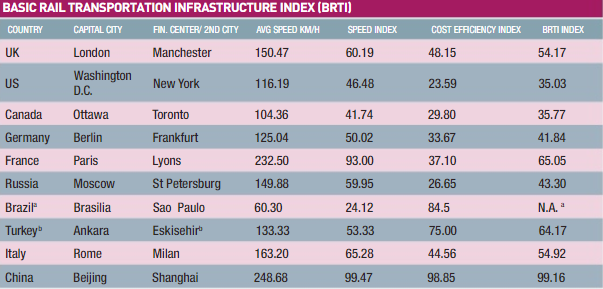
\includegraphics[width=\linewidth]{images/brti.png}
    \caption[Basic Rail Transportation Infrastructure Index]{BRT index}
	\label{fig:brti}
\end{figure}
    
Az általuk kiszámolt BRT index valóban alátámasztotta ezt, amint látható az \ref{fig:brti} ábrán, eredményeiket alátámasztja a stabil fejlődő gazdaságok igen csak magas indexel rendelkeznek.
Látható hogy gyengén fejlesztett vasút hálózatok esetén legtöbbször az index kiszámítása sem lehetséges. 
Tehát a globalizáció korszakában nyilvánvaló hogy a vasúti hálózatok jövője a fejlesztések folytatásával és ezen tudás megosztásával áll szoros kapcsolatban. 

\subsection{A dolgozat témája}\subsectionro{Tematica lucrării}
A dolgozatom témája egy modell vasúti hálózat automatizálásának megvalósítása. Tanulmányozva az iparban használt implementációs elveket, és ahol lehetséges ezekre az elvekre támaszkodva felépíteni a rendszert. Négy fontosabb részre oszthatjuk a rendszerünk amint látható a \ref{fig:realizedsys}. ábrán:
\begin{enumerate}
    \item A központi vezérlés: egy mikrokontroller figyel a hálózatban található többi mikrokontrollere és továbbítja egy számítógépre telepített vezérlő szoftvernek az érkező adatokat. A kommunikáció rádiófrekvencián történik és két irányú.
    \item A mozdony vezérlő: egy mikrokontroller segítségével megvalósítja a mozdonyban található DC motor sebesség vezérlését, valamint parancsokat fogad a központi vezérléstől.
    \item A jelző  hálózat: egy mikrokontroller segítségével megvalósítja a vasút rendszerekben használt jelző lámpák aspektusának a beállítását, a vezérlő adat ugyancsak rádiófrekvencián érkezik a központi vezérléstől.
    \item Az észlelő hálózat:  egy mikrokontroller segítségével megvalósítja a mozgásban levő szerelvény topológiai helyzetét, majd ezt az adatot továbbítja rádiófrekvencián keresztül a központi vezérlésnek.
\end{enumerate}

\begin{figure}[htp]
    \centering
	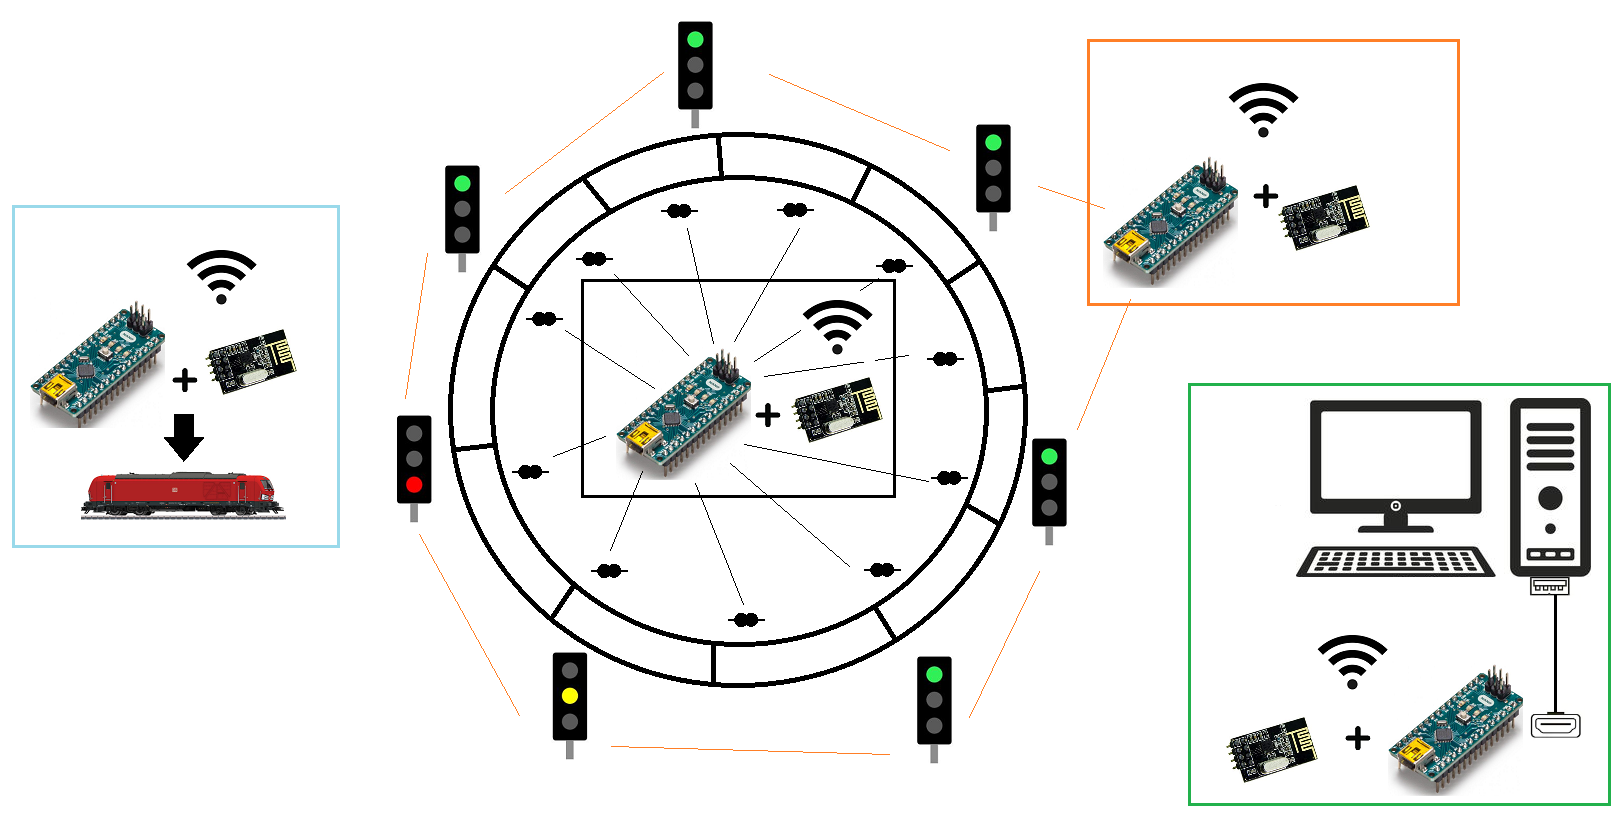
\includegraphics[width=\linewidth]{images/realizedsys.png}
    \caption[Megvalósított rendszer elvi rajz]{Megvalósított rendszer}
	\label{fig:realizedsys}
\end{figure}
%2
\section{Szakirodalmi tanulmány}\sectionro{Studiu bibliografic}\label{RAbasics}

A szakirodalmi tanulmány első sorban egy pár, a szakmában, nélkülözhetetlen könyvre épül.
A \textit {Joern Pachl: A vasúti üzemeltetés és ellenőrzés} \cite{jp09} és a \textit {Gregor Theeg, Sergej Vlasenko: Vasúti jelzés és biztosítóberendezések} \cite{gtsv18}, valamint a \textit{Peter Stanley: ETCS mérnököknek}\cite{ps11} című könyvek szinte kötelező irodalomként vannak számon tartva a vasúti elemek valamint logika fejlesztésének az ágazataiban. 
Értelemszerűen az elkövetkező fejezetek ezen könyvek tartalmának megemésztésével, újra fogalmazásával valamint magyar nyelvre való fordításával készültek el, kiegészítve a szakmában gyakran referált cikkekkel.

\subsection{Vasútrendszerek specifikációi}\subsectionro{Spețificațiile a sistemelor feroviare}
\textit {Jochen Trinckauf} szavait értelmezve az összes vasút rendszer esetében a következő két specifikációt azonosíthatjuk:
\begin{enumerate}
    \item A vonat által követet útvonalat a kerék és a sín mechanikai irányítása határozza meg, és ez az útvonal csak egy kitérő ( speciális vasúti elem) beavatkozásával változhat.
	Ebből kifolyólag lehetőség kell legyen egy ilyen rendszerben az útvonal beállításra, mivel a kitérők több lehetséges útvonalat megvalósítanak. Nyilvánvalóan egy vágányos rendszerek esetén, az irányváltoztatás zárt hurok használatával is megvalósítható. 
    Mivel a jármű szoros kapcsolatban áll az irányító rendszerrel, a vasúti rendszerek lineáris/szekvenciális rendszerekként is azonosíthatóak. 
	\item Az acél alapú vasúti kerekek relatív gyenge fékező képességgel rendelkeznek az ugyancsak acél alapú síneken. 
	Ebből kifolyólag a vezető által látható útvonalon kívül szükség van további elővigyázatossági intézkedésekre, annak érdekében hogy időben tudjon a vezető döntést hozni a sebesség csökkentésére vagy a vágány szakasz elhagyására vagy a teljes megállásra.
\end{enumerate}
\par Tehát ezekből azt a következtetés vonható le hogy, a vasúti rendszerekben esszenciális a helyes jelzés és vezérlés. 
A hálózat menedzser részéről fontos tudnia hogy egy adott időpontban pontosan hol, mikor és meddig van a gördülő állomány.
Annak érdekében hogy tudjon egy optimális és gazdaságos menetrendet szerkeszteni. 
Valamint a mozdony vezető - diszpécser - operátor szemszögéből fontosak ezek az elemek ahhoz hogy biztonságos, elérhető és karbantartott legyen a vasúti rendszer.
\pagebreak
\subsection{Vasúti elvek és standardok}\subsectionro{Principii și standarde feroviare}
Kibővítve a korábbi specifikációkat vasút rendszereknek három fontos részük van:
\begin{itemize}
	\item \underline{Infrastruktúra}, ami magában foglalja a teljes sin hálózatot/pályákat, állomásokat, és az ezekre szerelt mechanikus és/vagy elektromos felszerelést
	\item \underline{Gördülőállomány}, amely a mozdonyok és szerelvényeket képezi, fügétlenül attól hogy közszállítási vagy ipari szállításban használódik
	\item \underline{Üzemeltetési szabályok}, pontosabban a hálózatban használt működési szabályokat és eljárásosakat értjük ez alatt
\end{itemize}
\par Egyszerűség kedvéért az infrastruktúrát és gördülőállományt nevezhetjük a rendszer \textit{hardverének}, valamint az üzemeltetési szabályokat a \textit{szoftverének}.
Egy specifikus alrendszer az úgy nevezett automatikusa vonatvédelmi rendszer (\textbf{Automatic Train Protection}, továbbiakban \textbf{ATP}) felelős az egyik legfontosabb funkcióért a vasúti rendszerekben.
Az ATP szerepe az hogy információt továbbítson az útvonalról a mozdony vezetőhöz és automatikusan megállítsa a mozgó járművet ha emberi mulasztás miatt nem vesz figyelemben egy erre utaló jelzést a központi forgalom irányítótól. 
Ez az alrendszer tehát kapcsolatot teremt a gördülőállomány és az üzemeltetési szabályok között, információt szolgáltatva az infrastruktúrán található egyéb járművekről.
Feltalálása áttörő szerepet játszott a vasúti balesetek csökkentésében és/vagy szinte teljes elkerülésében. Sajnálatos módon az ATP rendszer implementációja nagyon nagy variációnak örvend.
Az európai országok közötti üzemeltetési szabályok annyira különbözőek voltak, hogy a 90-es évek végén több mint 14 különböző nemzeti standardot letehet azonosítani. 
Gyakorlatban szinte minden ország saját szabályokat alkalmaz, ennek az a negatív következménye hogy nagyon megnehezíti az átjárhatóságot az országok között. 
Az Európai Unió megalakulásának és idővel terjedésének köszönhetően, gazdasági okokból szükségszerű lett ezt a problémát megoldani. Mivel rengeteg idő és pénzügyi veszteséggel jár
minden országhatárnál mozdonyokat cserélni vagy készenlétben tartani határon túli szállítmányok esetén. Valamint ugyancsak magas költségel jár egy mozdony felszerelése több ország ilyen rendszerével.
Továbbá a nagy sebességű vonat hálózatok megjelenése, mint például a francia \underline{TGV}, a létező vezérlési technológiát is elavultnak tekintette.
Ezeknek következménye volt az \textbf{ERA - European Rail Agency} vagyis az \textit{Európai Vonat Ügynökség} megalakulása. 
Pár éven belül megalkották az átjárhatóságot lehetővé tevő technikai specifikációt, felkarolva az elődjét az \textbf{ERTMS - European Rail Traffic Management System}-et \textit{(Európai Vasút Forgalom Menedzsment Rendszer)}.
Az ERTMS komponenseként jött létre az \textbf{ETCS - European Train Control System}-et \textit{(Európai Vasút Vezérlési Rendszer)}.
Az ETCS szolgáltatja a technikai megoldásokat legtöbb új fejlesztésű vagy megújításra kerülő vasúti rendszereknek.
Idővel amint a megoldások bizonyították életképességüket,a kivitelezési folyamatot a \textbf{CENELEC} intézmény által standardizálták is.
\subsubsection{ETCS}\subsubsectionro{ETCS}
Az ETCS projekt célja hogy fokozatosan a hagyományos ATP rendszereket Európa szerte egy egységes két irányú kommunikációra képes vonat vezérlő rendszerre cserélje le.
Fontos megjegyezni hogy az újítás mindhárom vasút rendszeri komponenst érinti (Infrastruktúra, Gördülőállomány, Üzemeltetési szabályok).
Az új rendszerben új technológiákat vezettek be mint az \textbf{"euro-balise" (magyarul euró-pályamágnes)} vagy a GSM-R alapú kommunikáció. 
A pályamágnesek szerves részét képzik az ETCS technológiának, lényegében a sínek között elhelyezett jeladó szerkezet. 
Az az amikor egy ETCS rendszerrel felszerelt mozdony halad el fölötte információt továbbit a pályamágnes után következő útvonalról. Nagy előnye hogy statikus adat továbbítás esetén nem igényel külső áramforrást.
A kommunikáció típusától függően több szintre osztották az új megközelítéseket. 
Továbbiakban ezeket nézzük meg közelebbről.


\begin{itemize}
	\item \textit{0 szint} Ez a szint egy átmeneti állapotot ír le, az az eset amikor egy ETCS képes jármú egy non-ETCS hálózatban közlekedik.
	Egy ilyen szcenárióban a gördülőállomány maximum sebesség minimumával halad a hálózatban, és  emellett egy nemzetileg meghatározott 0 szintes sebesség korlátot is be kell tartania.	
	
	\item \textit{1 szint} Ezen a szinten az ATP egy fejlesztett időszakos verzióját találhatjuk és a pályamágnes az integrális fő adat átadási csatorna.
	Lényegében a pályamágnes, az érkező ETCS mozdonynak, mozgás engedélyt és profiladatokat továbbit.A pályamágnes lehet rögzített adat továbbító vagy váltható. 
	Míg az első csak statikus adatot továbbit ( például: földrajzi pozíció), addig  a második legtöbbször egy vonal menti elektromos készülék befolyására dinamikusan megválasztott adatot továbbit ( például: jelző aspektus).
	A pályamágnesek általában csoportokban vannak összekötve, így észlelhető ha valamelyik meghibásodik, valamint a csoport végső tagja képes információt továbbítani a következő csoport első tagjának.
	A csoportok közötti kommunikáció keretantennával bővülhet amely rádió frekvencián képes adatokat továbbítani, ezek az úgy nevezet Euroloop-ok.
	Érezhető hogy így relatív gazdaságosabban nagy távokat le tudnak fedni, lényeges vasút hálózat adatokat szolgáltatva.
	A harmadik lehetséges adat áramlás a helyváltoztatási adat, ezt az észlelő hálózat gyűjti be, az óvórendszer feldolgozza, és megfelelő jelző aspektust állít be, a biztonságos továbbhaladás érdekében.
	A járműn található ETCS berendezés ezen adatok alapján valós időben számol helyzetet, biztonsági féktávot, valamint egy sebességet amit közöl a vezetőnek.
	Ezt az elvi működést láthatjuk a \ref{fig:etcslevel1}. ábrán. Ez az alszinten valósítja meg a  teljes felügyelet módot. 
	Mivel az ETCS rendszer megszakítás nélkül felügyeli az összes befolyásoló paramétert.	
	\begin{figure}[htp]
	    \centering
	    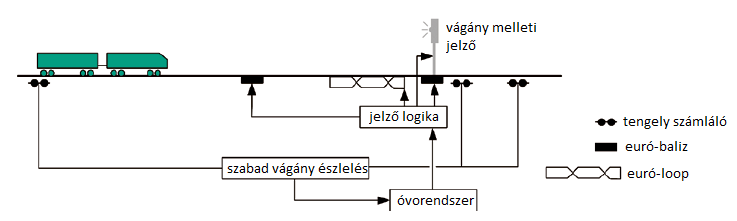
\includegraphics[width=\linewidth]{images/etcs_level_1.png}
	    \caption[ETCS 1]{Adat folyam ETCS 1 szinten}
	    \label{fig:etcslevel1}
    \end{figure}
	
	Létezik viszont korlátozott felügyeleti mód is. Ez abban az esetben fordulhat elő, ha egy olyan jelző berendezéssel találkozik a jármű amely megállási aspektust mutat a vezetőnek.
	Ilyenkor egyéb ETCS rendszer nem szolgál más adattal, a vezető kénytelen ebben a módban megvárnia az aspektus változást ahhoz hogy tovább haladjon.
	
	\item \textit{2 szint} Egy folytonos ATP rendszerként működik. Ebben az esetben a vonat vezérlő adat GSM-R rádió frekvencián van továbbítva.
	A pályamágnesek továbbra is használtak, viszont döntő többségben statikus adatot szolgáltatnak az áthaladó szerelvénynek, szerepük elektromos vasúti mérföldköre hasonlítható.
	Adott egy adó vevő központ az RBC (Radio Block Center - Rádió Blokk Központ) amelynek a vonat ciklikus idő közönként (általában 60 másodperc) továbbítja a helyzetét meg paramétereit. 
	Válaszként pedig az RBC továbbítja a szükséges továbbhaladási jogokat, valamint egyéb biztonsági paramétereket.
	Vonal menti jelző készülékekre elvileg már nincs szükség csak vonat választási mozgások esetén. 
	Ez esetben a jól bevált észlelő és jelző technológiák használata igényelt, valamint degradált operációs módban szükség lehet erre (pl: non ETCS gördülőállomány hajt be az ETCS hálózatban).
	A \ref{fig:etcslevel2}. ábrán az ETCS 2-es szint egyik lehetséges adatfolyama látható. 
	
	\begin{figure}[htp]
	    \centering
	    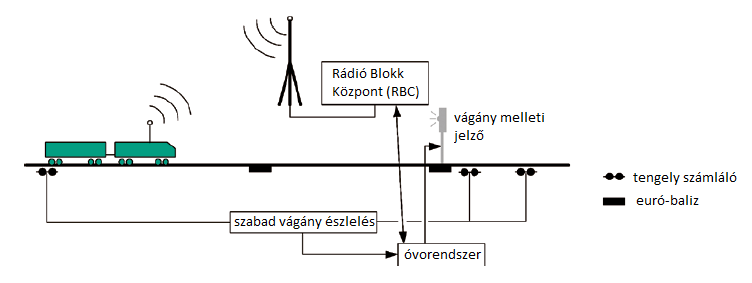
\includegraphics[width=\linewidth]{images/etcs_level_2.png}
	    \caption[ETCS 2]{Adat folyam ETCS 2 szinten}
	    \label{fig:etcslevel2}
    \end{figure}
    
	\item \textit{3 szint} Végül a \ref{fig:etcslevel3}. ábrán látható adatfolyam jellemző a hármas szintre. Ez esetben bevezetődik a vonat integritás fogalma.
	Hármas szinten garantált kell legyen a gördülőállomány egységessége. 
	Ennek segítségével már elégséges az RBC kommunikáció és pályamágnesek használata, mivel garantáltan tudjuk a jármű hosszát a hálózatban és a hálózat paramétereit.
	Valamint az RBC és jármú közötti kapcsolat folytonos. Ezzel a módszerrel sem észlelő sem jelző berendezésekre nincs már szükség. 
	
	\begin{figure}[htp]
	    \centering
	    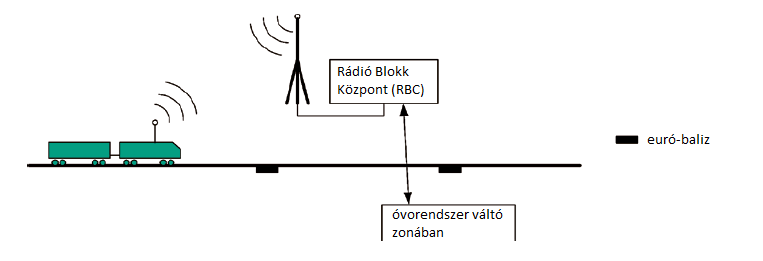
\includegraphics[width=\linewidth]{images/etcs_level_3.png}
	    \caption[ETCS 3]{Adat folyam ETCS 3 szinten}
	    \label{fig:etcslevel3}
    \end{figure}	
\end{itemize}

Napjainkban döntő többségben ETCS egyes és kettes szintű vasúti projektek vannak használatban vagy kivitelezési folyamatban. 
Az ETCS hármas szintet csak pár regionális ETCS rendszerben tesztelik. Gondot okoz az utóbbinál a vonat integritás kérdése. 
Még nem sikerült egy gazdaságos és standardizálható technikai megoldást találni amely minden körülmény között garantálni tudja a vonat szerelvények egységességét. 

\subsubsection{CENELEC}\subsubsectionro{CENELEC}\label{cenelecchapter}
    \begin{wrapfigure}{r}{0.30\textwidth}
        \vspace{-20pt}
        \centering
        
\includegraphics[scale=0.4]{images/CENELEC_logo.png}
        \caption[CENELEC logo]{CENELEC logo}
        \label{cenelec_logo}
    \end{wrapfigure}

A CENELEC (francia: \textbf{Comité Européen de Normalisation Électrotechnique}) - \textit{Európai Elektrotechnikai Szabványügyi Bizottság} [\ref{cenelec_logo}] egy belga szervezet amely európai standardok megalkotásával foglalkozik az elektromos mérnöki ágazatban. 
Annak ellenére hogy magas mértékben közreműködik az Európai Unió intézményével, nem része ennek.
A különböző ipari és technikai ágazatokban működő uniós ügynökségekkel és magán csoportokkal/konzorciumokkal együttműködve fekteti le az illetékes ágazat európai szintű standardjait.

A vasúti rendszerek kivitelezésében első sorban a biztonságra és kivitelezési folyamatra helyeznek ezen standardok nagy hangsúlyt.

Az EN5012x CENELEC normák érintik a vasúti rendszereket, és a következő standardokat tekinthetjük a legfontosabbaknak:
\begin{itemize}
	\item \textbf{EN 50126} - R.A.M.S. röviden, a vasúti rendszer életciklusát követi különböző szemszögekből, talán a legszervesebb része a vasúti normáknak
	\item \textbf{EN 50128} - A vasúti szoftver alrendszerek életciklusát tárgyalja
	\item \textbf{EN 50129} - Szoros kapcsolatban áll az EN 50126-os normával, további biztonsági folyamatokat szögez le a vasúti jelző rendszerre kitérve, S.I.L.
\end{itemize}



Az EN 50126 norma szerint a vasúti rendszer fejlesztése működtetése/ karbantartása és végül leszerelése egy megtükrözött vízesés módszertanhoz hasonlít.
Amint látható a \ref{fig:cenelec_vmodel}. ábrán ez lényegében a "V" betűre hasonlít, épp ezért is nevezték el V modellnek.

\begin{figure}[htbp]
	\centering
    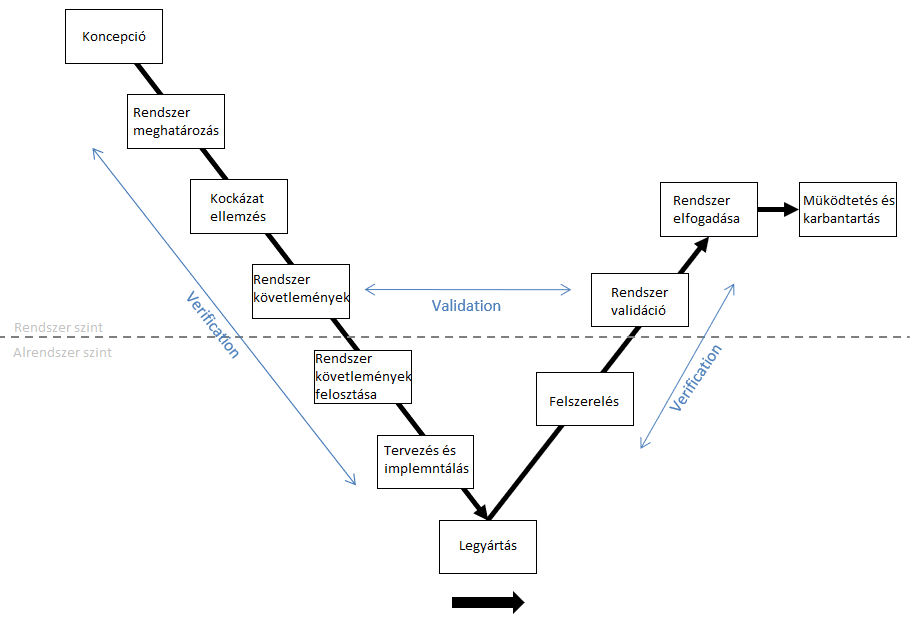
\includegraphics[width=\linewidth]{images/CENELEC_vmodel.png}
    \caption[V modell] {V modell EN 50126 szerint}
    \label{fig:cenelec_vmodel}
\end{figure}

A modell részletes működése és használata nem célja ezen dolgozatnak, éppen ezért nem térünk ki rá bőven. Az rendszer életciklus lépései elég beszédesek ehhez.
Megjegyzendő viszont a verifikáció és validáció fogalma a V modellben. 
Legegyszerűbb értelemben a verifikálási folyamat a \textit{Helyesen építjük ezt a rendszert?} valamint a validációs folyamat a \textit{A kivitelezés megéri? Képes elvégezni a feladatot?} kérdésekre kell megadja a választ.

\begin{wrapfigure}{r}{0.40\textwidth}
    \vspace{-20pt}
    \centering
    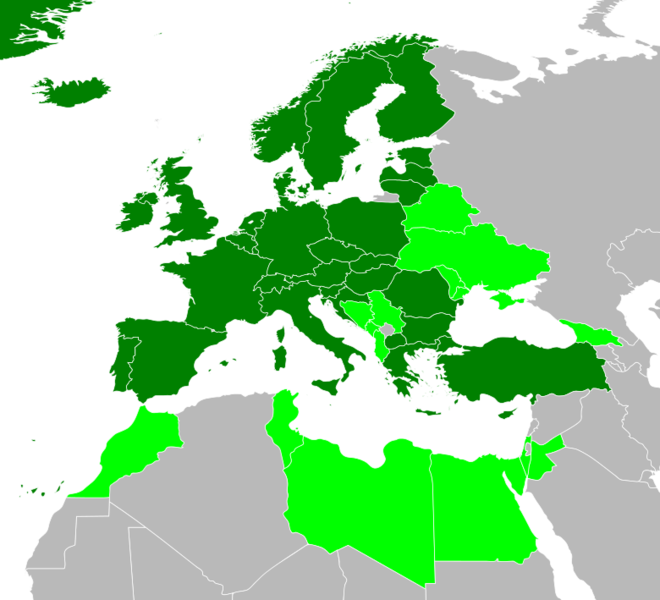
\includegraphics[scale=0.8]{images/CENELEC_membership.png}
    \caption[CENELEC tagországok]{CENELEC tagországok}
    \label{fig:cenelec_members}
\end{wrapfigure}

Természetesen ezek a standardok nincsenek korlátozva csak európai országokra. 
Amint láthat a \ref{fig:cenelec_members}. ábrán vannak országok amelyek speciális egyezményeket kötöttek és használják saját országaikban is ezeket. 
Ezen túl globálisan is használatban vannak olyan országokban mint Kína, Kanada, Japán, Oroszország, India vagy az Egyesült Államok.

\subsubsection{R.A.M.S.}\subsubsectionro{R.A.M.S.}

Ahogyan a korábbi fejezetekben említettük a vasúti rendszereknek van pár lényeges tulajdonsága. 
A \textbf{R.A.M.S} vagy néha \textbf{R.A.M.S.(S)} rövidítések ezen tulajdonságok összegzése angolul, és jelentése a következő:

\begin{itemize}
	\item {\huge R}\textbf{eliability} -  \textbf{Megbízhatóság}
	\item {\huge A}\textbf{vailability} - \textbf{Elérhetőség}
	\item {\huge M}\textbf{aintainability} - \textbf{Karbantarthatóság}
	\item {\huge S}\textbf{afety} - \textbf{Biztonság}
	\item {\huge S}\textbf{ecurity} - \textbf{Védelem}
\end{itemize}

Fontos leszögezni hogy ezek a fogalmak mit is jelentenek konkrétan vasúti rendszerek kontextusában.
A \textbf{Biztonság} alatt a szó szerinti funkcionális biztonságot értjük, szerepe védelmet nyújtani veszélyes eseményekre. 
Ez lehet technikai hibásodás, de akár nem szándékos emberi hiba is.
A \textbf{Védelem}, ezzel ellentétben , arra szolgál hogy megelőzzön veszélyes következményeket a vasúti rendszere szándékos, észszerűtlen emberi beavatkozás ellen.
A két fogalmat fontos külön értelmezni. Például egy vészkijárat tökéletes analógia erre. 
Ahhoz hogy vészhelyzet esetén használható legyen, az ajtó belülről egyszerűen nyitható kell legyen, tehát zár nélkül. Ez egy biztonsági kérdés.
Viszont ahhoz hogy illetéktelen személy ne tudjon behatolni, ugyanaz az ajtó kívülről zárt kell legyen. Ez egy védelmi kérdés.
Vasúti rendszerekben is hasonló kontextusban értelmezzük ezeket a fogalmakat. Maga a rendszer és ehhez hozzá tartozó komponensek meg kell hogy oldják a biztonság kérdését.
De védelmet is kell biztosítani a rendszeren belül, hogy illetéktelen személyek ne tudjanak hozzá férni és veszélyes eseményeket előidézni.

A megbízhatóság, elérhetőség és karbantarthatóság hatnak egymásra (lásd  \ref{fig:ram_dependency}. ábrát).

\begin{figure}[htp]
	\centering
    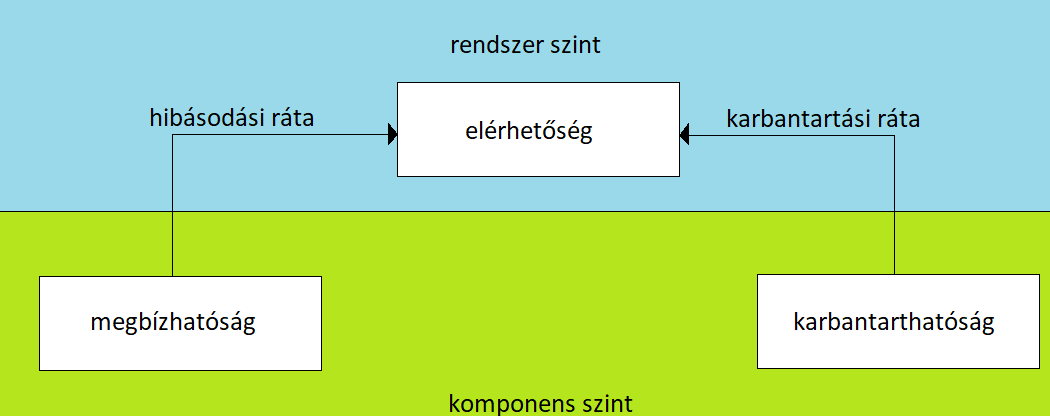
\includegraphics[width=\linewidth]{images/rams_dependency.png}
    \caption[R.A.M. függőség]{R.A.M. függőség}
    \label{fig:ram_dependency}
\end{figure}
\textbf{Elérhetőség} alatt a rendszernek egy olyan képességét értjük amely által képes elvégezni, egy adott időpontban vagy időintervallumban, a neki kiadott feladatot.
Természetesen akkor ha adott a megfelelő keretrendszer ezen feladat elvégzéséhez.
Egy lényeges funkciója a vasúti rendszereknek személyek és árú szállítása biztonságos körülmények között.
Ezért szükségesek előfeltételek, külső segítség források formájában, amelyeknek köszönhetően elvégezheti ezt a feladatot.
Például ez lehet a megbízható technikai komponensek melyek alkotják a rendszert ( óvórendszer, jelző vagy észlelő készülék), de ugyanakkorra mértékben ide tartozik a rendszert működtető személyzet is. 
Tehát a megbízhatóság egy fontos befolyásoló tényezője az elérhetőségnek. 
\textbf{Megbízhatóság} alatt a vasút rendszerben azt a valószínűséget értjük, hogy egy komponens, egy adott időintervallumban, elvégzi a követelmények által meghatározott feladatát.
Ez hiba mentes működéshez vezet. Amikor ez a valószínűség nem jön létre beszélünk hibásodásról, ennek gyakorisága pedig adja meg a hibásodási rátát.
Ezt azt jelenti hogy rendszerünk nem lesz elérhető, ez vezet tehát a karbantarthatósághoz.
\textbf{Karbantarthatóság} is egy valószínűség, amely szerint egy javítási kísérlet egy adott idő intervallumban, kivitelezhető.
Integrális követelmény egy vasútrendszerben a magas elérhetőségi szint. 
Fentiek alapján láthatjuk, hogy ahhoz hogy ez megvalósuljon szükséges a meghibásodási rátát alacsonyan, valamint a karbantartási rátát magasan tartani.

\subsubsection{S.I.L. szintek}\subsubsectionro{Nivele S.I.L.}
Az EN 50129 CENELEC standard egyik fő következménye a veszélyességi ráta leszögezése.
Ez az úgynevezett \textbf{Safety Integrity Level - S.I.L.} vagyis \textit{biztonsági integritás szint} formájában valósul meg.
Egyszerűen fogalmazva elfogadható veszélyességi rátát jelképez, amely függvénye a hibásodások által eredményezett kockáztok csökkentésének, valamint ezek gyakoriságának.
Tehát a vasúti rendszer kockázatoknak van kitéve, ennek pedig két befolyásoló paramétere a súlyosság és a frekvencia vagy előfordulási gyakoriság.
Szükségesé válik ezen kockázatok csökkentése. Ezt új, biztonságosabb technólogikákkal, vagy újabb biztonsági függvények hozzá adásával a rendszerhez, vagy a környezeti tényezők módosításával érhetjük el.
Az említett folyamatok alkalmazásával elérhetünk egy elfogadható kockázat határt.
Ezt a gyakorlatban a CENELEC norma leírja hogy milyen adatok feldolgozásával érhetjük el. 
A tézisnek nem célja hogy ezeket a komplex számításokat elemezzük, épen ezért csak röviden tárgyaljuk a folyamatot.
Az operátor (másképpen a vasúti rendszer megrendelője) kötelező módon végez egy kockázati elemzést, amit a gyártó rendelkezésére bocsájt.
Közösen azonosítják a potenciális veszély tényezőket, ezeket kielemzik és végül, az eredmények alapján, a rendszer különböző komponenseihez biztonsági követelményeket rendelnek.
A minőségi biztonsági követelmények reprezentatívak a S.I.L. szintre tekintve.
A gyártó tapasztalat, tesztek sokasága és statisztikai adatok alapján a rendszer legtöbb altkomponensére azonosít egy lehetséges óránkénti meghibásodás rátát.

\begin{table}[!htbp]
    \centering
    \begin{tabular}{|c|c|}\hline
        THR/óra és fügvény & S.I.L. szint \\ \hline
        $10^{-9} \leq THR < 10^{-8}$ & 4 \\ \hline
        $10^{-8} \leq THR < 10^{-7}$ & 3  \\ \hline
        $10^{-7} \leq THR < 10^{-6}$ & 2 \\ \hline
        $10^{-6} \leq THR < 10^{-5}$ & 1 \\ \hline
    \end{tabular}
    \caption[S.I.L szintek]{THR gyakoriság és a hozzá rendelt S.I.L szintek}
    \label{sil_levels}
\end{table}

Ebből kiindulva számolnak egy elfogadható veszélyességi rátát, amit a szakirodalomban \textbf{THR} ( -  \textit{angol: Tollerable Hazard Rate})-nek neveznek.
Így egy, habár kicsi de mérhető mennyiséggel dolgozhatunk. 
Ezen mérték függvényében 4 S.I.L. szintet határoztak meg, az egyes szint jelképezve a kevesebbe kockázatos elemeket, míg a négyes szint a legkritikusabb befolyással rendelkező komponenseket (\ref{sil_levels}. táblázat).

Például két vonat ütközése egy vonalon katasztrofális eseménynek számít.
Éppen ezért a biztosító rendszer, a jelző rendszer meg az észlelő rendszer pontos és beszámítható működésének kritikus szerepe van egy ilyen esemény elkerülésében. 
Tehát a rendszer ezen komponenseit 4-es szintű S.I.L besorolás alá helyezik. 
De viszont egy autó ütközése vasúti sorompóval, amíg nem kerül a vágányra, habár kockázati tényező nem sodor veszélybe direkt módon emberi életet, ezért ez a komponens csak 1-es szintű besorolás alá kerül.

\subsection{Vasút működtetési elemek és folyamatok}\subsectionro{Elemente și procese de operare a sistemelor feroviare}

A vasúti rendszerek működésének megértéséhez fontos megismerni a rendszer fő \textit{hardver} és \textit{szoftver} komponenseit. 
A \ref{fig:rail_topology_eg}. ábrán egy ilyen rendszer szimbolikus topológiai rajzát láthatjuk a fontosabb komponensekkel. 
A következő alfejezetek ezen szerves komponenseket tárgyaljuk röviden.

\begin{figure}[htp]
	\centering
    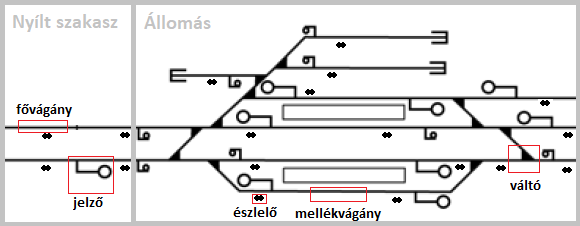
\includegraphics[width=\linewidth]{images/rail_topology_eg.png}
    \caption[Vasúthálózat topológia]{Vasúthálózat topológia és fő komponensei}
    \label{fig:rail_topology_eg}
\end{figure}
Legtöbb esetben a vasúti pályát két jól elkülöníthető  részre oszthatjuk.
Állomásokra és az ezek közötti nyílt szakaszra.

\subsubsection{Vágányok és jelenlét érzékelők}\subsubsectionro{Căi ferate și detectoare de prezență}
A vágány a vasúti hálózatok útteste. Az \ref{fig:rail_track}. ábrán látható struktúra szerint, ballasztra helyezett betonlapokból és sínpárból épül fel.

\begin{wrapfigure}{r}{0.3\textwidth}
	\vspace{-20pt}
	\centering
	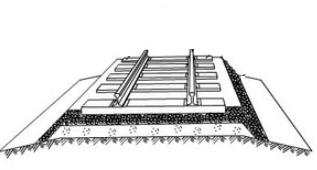
\includegraphics[scale=0.5]{images/rail_track.png}
	\caption[Vágány struktúra]{Vágány struktúra}
	\label{fig:rail_track}
\end{wrapfigure}

Amint látható a sínpár között van egy jól meghatározót, úgy nevezett, nyomtávolság.
A nyomtávolság standard mérete \textit{1435 mm}, ez annak a következménye hogy a globális vasúthálózat több mint 2/3-a ezt a méretet használja.
Éppen ezért is nevezzük standard méretnek. A vágány és ennek alapja hálózatokban rendezése, eredményezi a vasúti pályák kialakulását.
Alap értelmezetten ez a rendezés a következő típusú elemekből épülhet fel:
\begin{itemize}
	\item \textbf{Fő pálya} - Ez teszi ki a pálya nagy részét, itt haladnak a gördülő állományok jellegzetesen nagyobb sebsebéggel
	\item \textbf{Mellék pálya} - Legtöbbször állomásokon vannak használatban, a járművek speciális mozgásainak elvégzésére, valamint peronok kialakítására is szolgál
	\item \textbf{Kitérő/Váltó} - Mivel a vasúti jármű legtöbbször kényszer pályán halad, szükség van kitérők használatára ahhoz hogy módosítani tudja ezt a pályát.
	A váltószerkezet működtetése kritikus komponens, mivel frontális ütközéshez vezethet helytelen használat esetében. 
	Napjainkban ez a komponens egy elektromechanikus szerkezet, mely minden esetben visszatér eredt állapotában miután az pálya választást lehetővé tette a jármú számára.
	\item \textbf{Kereszteződés} - Olyan esetekben szükséges az implementációja amikor a hálózatban két főpálya keresztezi egymást.
	Jellegzetesen átlósan négy váltó határolja, amelyek párban kapcsolnak garantálva azt hogy egy adott időpontban csak egy vonat haladhat át a kereszteződésen.
\end{itemize}

\begin{figure}[htp]
    \centering
    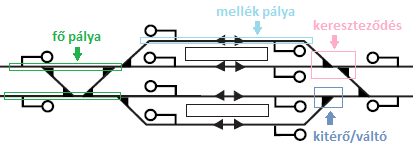
\includegraphics[width=0.5\linewidth]{images/rail_track_types.png}
    \caption[Vasúti pálya komponensek]{Vasúti pálya komponensek}
    \label{fig:rail_track_type}
\end{figure}

A vágánynak egy igen fontos kiegészítő komponense, az ETCS elvek szerint, az úgy nevezett észlelő rendszerek. 
Ezeknek szerepe értesíteni az operátort arról hogy jármű jelenlétet detektáltunk a vágányon. 
Az észlelő rendszereknek funkciói ezen információ észrevétele, továbbítása és feldolgozása.
Ennek két általánosan elterjedt verziója van használatban:
	\begin{figure}[htp]
		\centering
		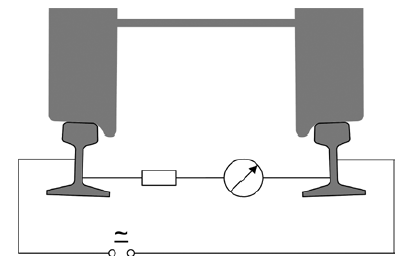
\includegraphics[width=0.5\linewidth]{images/track_circuit.png}
		\caption[Pályaáramkör működési elv]{Pályaáramkör működési elv}
		\label{fig:track_circuit}
	\end{figure}
\begin{itemize}
	\item \textbf{Pályaáramkör} A működési elve a sönt ellenálláséra hasonlít.
	Egy adott pályaszegmens mindegyik sínére egy áramforás egyik egyik pólusát csatlakoztatják. Az áthaladó vonat kerék és tengely páros megnöveli a sönt ellenállást az áramkörben [\ref{fig:track_circuit}].
	Ezt egy szenzor érzékeli és továbbítja az adatot a biztosító rendszernek. Előnye hogy nagyon egyszerű és viszonylag olcsó.
	Viszont van egy kritikus hátránya, ha az áramkör valamilyen okból kifolyólag megszakad vagy az ármarforrás kisebb feszültséget szolgáltat, akkor hibásan jelezhet szabad vonal szegmenst, amikor ez mégis foglalt.
	Ebből kifolyólag ritkán, vagy csak vonat parkoló hálózatokban, használt legtöbbször. Mivel itt kis sebességgel haladnak a járművek, nem kritikus a biztonság.
	
	\item \textbf{Tengely számlálok} A tengely számlálok rezonancia áramkörökre épülnek. A sin mindkét oldalán elhelyeznek egy indukciót generáló adó-vevő rezonancia áramkörpárost [\ref{fig:axle_counter}].
	Ez létrehoz a két áramkör között egy mágneses mezőt. Abban a pillanatban amikor egy szerelvény kerék áthalad ebben a mágneses mezőben, módosul az áramkör induktivitása. 
	Ez a módosulás amplitúdó növekedéshez is vezet a vevő oldalon. Ezt érzékelve, és mivel ugye a kerék a tengelyhez van rögzítve, minden áthaladó tengely egy impulzust fog létre hozni.
	Tehát minden impulzus egy áthaladó tengelyt jelent, ezt az adatot pedig továbbítja a helyszíni feldolgozó egységnek.
	A tengelyszámlálók párban vannak felszerelve a vágány mellet. 
	\begin{figure}[htp]
		\centering
		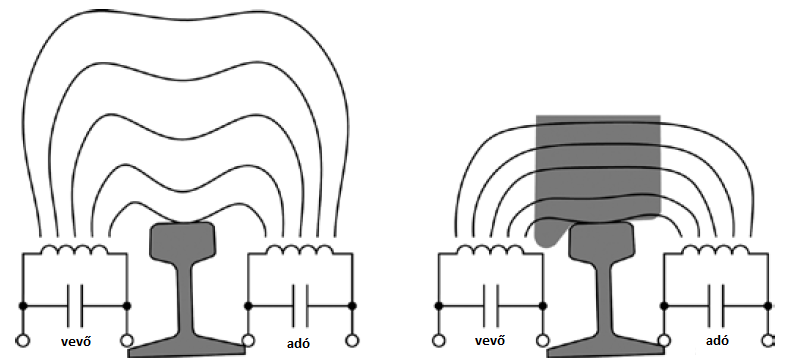
\includegraphics[width=\linewidth]{images/axle_counter.png}
		\caption[Tengely számláló működési elv]{Tengely számláló  működési elv}
		\label{fig:axle_counter}
	\end{figure}
	A számláló pár pedig be van kötve a helyszíni vezérlő áramkörben, amely figyeli hogy az első számláló áramkör ugyanannyi tengelyt számolt mint a második.
	A biztosító rendszerhez csak ennek az összehasonlításnak az eredményét küldi tovább.
	A páros megoldás miatt, a haladási irányt is képes meghatározni.
	Előnyei hogy nem befolyásolják a környezeti tényezők, és hogy irányt is képes érzékelni, valamint nagyon kicsi a hibásodási rátája.
	Viszont komplexebb elektronikai készülékekre van szükség működtetéséhez, amelyek drágábbak mint a pálya áramkörök.
\end{itemize}
A pályaáramkör egy direkt észlelési módszer, mivel a vágányhálózathoz csatlakozik.
Ezzel szemben a tengely számláló indirekt módszer, mivel nem direkt része a vágány hálózatnak. 
Mindkét esetben a cél a vágány foglaltsági állapot pontos meghatározása, és továbbítása a biztosító rendszer felé.
Gyakorlatban többnyire tengelyszámláló fordul elő gyakrabban, mivel pontosabb, kevésbé befolyásolják külső tényezők valamint nem kell a pályát szigetelni a visszáramok miatt.

\subsubsection{Jelzők és jelző aspektus}\subsubsectionro{Semnalizatoare și aspecte de semnal}

A jelző készülékek szerepe az új ETCS megoldások miatt, kezd háttérben szorulni.
Legtöbb ETCS szinten opcionális vagy teljesen szükségtelen. 
Ezek ellenére rendkívüli feladat és hatalmas gazdasági erőfeszítést igényel egy ország teljes hálózatának az átépítése, egy magasabb ETCS szintre.
Gyakorlatban legtöbb esetben hibrid megoldásokat alkalmaznak.
Az az annak ellenére hogy ETCS elv szerint fejlesztik az új hálózatokat, megtartják a jelző készülékek használatát is, főleg állomások és vasúti kereszteződések esetén.

A jelzők szerepe hogy információt továbbítsanak az embereknek, itt első sorban a mozdony vezetőre gondolhatunk. 
De a hálózati menti alkalmazott személyzet számára is fontos lehet.
Ez az információ biztonsági okokból kritikus, mivel a vonatok fix vágányokon mozognak, az ütközés lehetősége igen magas.
Ez a hatalmas tömeg és inerciának köszönhető. Ugyanakkor ennek következménye hogy hirtelen akadály esetén, nehezen képes megállni.
A jelzők a következő fontosabb információkat továbbítják:
\begin{itemize}
	\item mozgási engedély
	\item megengedett sebesség
	\item kitérők helyzete
	\item közelgő vasúti kereszteződés
\end{itemize}

Fizikai korlátozások miatt, a jelző készülékek elhelyezése függ a vonat sebességétől.
Ezt három kategóriában soroljuk:
\begin{table}[!htbp]
    \centering
    \begin{tabular}{ |c|c|c| } \hline
        Pálya típus & Sebesség & Jelző pozíció \\ \hline
        Hagyományos szakasz & $\leq 60 km/h$ & Vágány mentén \\ \hline
        Gyors szakasz & $ \leq 200 km/h $ & Vágány mentén kiegészítéssel \\ \hline
        Magas sebességű szakasz & $ \geq 200 km/h $ & Mozdony kabinban\\ \hline
    \end{tabular}
    \caption[Jelző pozíció és sebesség]{Jelző pozíció és sebesség kapcsolat}
\end{table}
Értelemszerűen nagy sebesség esetén a mozdony vezető már, ha észre is veszi, nem tudom elég gyorsan reagálni az adott jelzésre.
Az ETCS elvek alapján ekkor a jelzés már a vezető rendelkezésre bocsájtott interfészen fog megjelenni.
Közepes sebességek esetén a fő jelző vonalakat kiegészítik távolsági jelző készülékekkel. 
Ennek szerepe hogy értesítse a vezetőt egy közelgő fő jelző állapotáról.
A jelzők legfontosabb biztonsági paramétere az aspektus. Ami nem jelent mást mint a jelző által kibocsájtott fény színéhez rendelt mozgás típus.
Ezt tekintően országonként változhat a segéd jelzések típusa és értelmezése.
Viszont a fő elv, az ETCS-nek megfelelően is, a \ref{tab:aspectandcolor}. táblázat szerinti értelmezést írja elő globálisan.

\begin{table}[!htbp]
    \centering
	\begin{tabular}{ |c|c| } \hline
		Szín & Aspektus \\ \hline
		fehér \cellcolor{white} & Tolatás \\ \hline
		piros \cellcolor{red} & Stop \\ \hline
		zöld \cellcolor{green} & Szabad \\ \hline
		sárga \cellcolor{yellow} & Figyelem \\ \hline
	\end{tabular}
	\caption[Jelzőszín és aspektus reláció]{Jelzőszín és aspektus reláció}
	\label{tab:aspectandcolor}
\end{table}
A jelző berendezés is alárendelt a szokásos ETCS és CENELEC biztonsági protokolloknak.
Ami ezt jelenti hogy kritikus befolyásoló jellege van, kommunikál a biztosító rendszerrel valamint az operátor interfésszel.

\begin{figure}[htp]
	\centering
	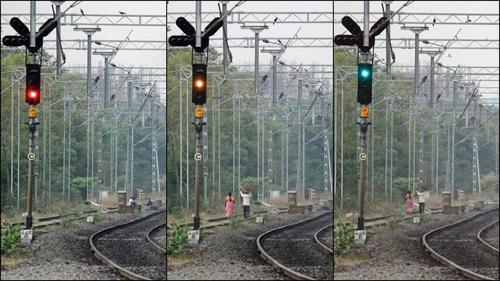
\includegraphics[width=\linewidth]{images/rail_signal_aspects.png}
	\caption[Jelző készülék]{Standard vasúti jelző készülék működés közben az alap aspektusokkal}
\end{figure}

\subsubsection{Vonat mozgások}\subsubsectionro{Tipuri de deplasare a trenurilor}
A vonatok áthaladását a vasúthálózaton, egy menetrendre alapuló, specifikus szegmensekre behajtási engedéllyel rendelkező utasítások sorozata.
A menetrend egy olyan beosztást is tartalmaz, amely az engedély mellet tartalmazza a bizonyos szegmens sebesség korlátozását is.
A vonatok, biztonsági okokból, hátsó lámpával vagy táblával is fel vannak szerelve.
Ezúton ellenőrzik sok esetben a szerelvény sorozat integritását.
A vonatmozgásokat két kategóriában soroljuk:
\begin{enumerate}
	\item \textbf{Normál vonat mozgás} - Az összes, állomáson kívüli, fő pályán történő mozgás ilyen típusú. 
	\item \textbf{Tolató mozgás} - Azon mozgások mely során a vonat vágányt vagy irányt cserél vagy szerelvényekkel bővül/csökken.
	Legtöbbször állomás területén belül történik, mellékpályákon, váltók és kereszteződések segítségével.
\end{enumerate}
Továbbá fontos megemlíteni a behajtási engedély forrását. 
Első sorban, jelzők által irányított pályán, ez a biztosító rendszer által szolgált jelző aspektus adja.
Ha \textit{STOP} aspektust mutat a jelző, a vonat tovább hajthat de csak abban az esetben ha felügyelő operátor verbálisan vagy írásban engedélyt ad erre.
Másod sorban ha nem jelzők által irányított pályán halad akkor a menetrend és operátor utasításai alapján történik a tovább haladás.

\subsection{Biztosító rendszerek}\subsectionro{Sisteme de cuplare/asigurare}
Ahogyan a korábbi fejeztek is referálták a \textbf{biztosító rendszer} ( \textbf{en: Interlocking}) egy kritikus része a vasúti rendszerek architektúrájának.
Lényegégben egy köztes szoftver réteg a vágány mellet készülékek és az operátor interfésze között.
Képes garantálni hogy az észlelő szenzorok által szolgált információ alapján, a jelző hálózat komponenseit egy szekvenciális és konfliktus mentes állapotban beállítva, biztosítja a hálózatbeli vonat mozgásokat.

\begin{figure}[htp]
	\centering
	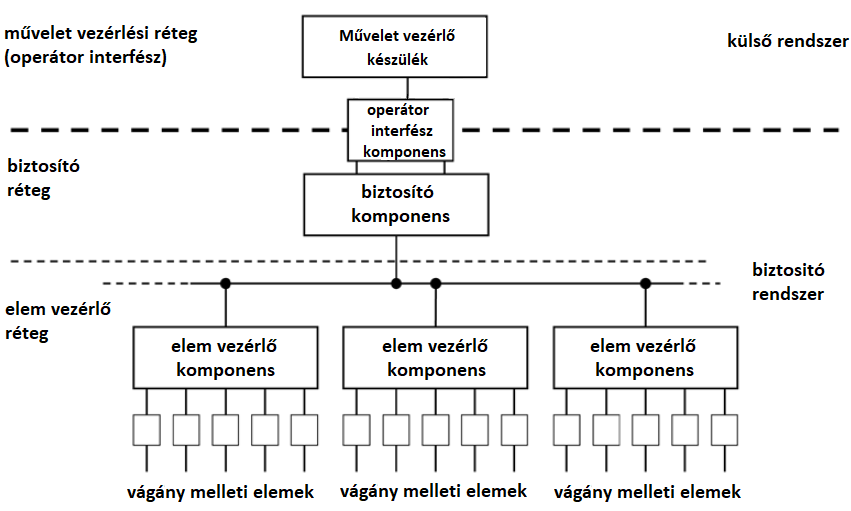
\includegraphics[width=\linewidth]{images/interlocking_functional_structure.png}
	\caption[Intrlocking funkcionális struktúra]{Elektromos biztosító rendszer funkcionális struktúrája}
	\label{fig:interlocking_functional_structure}
\end{figure}


Struktúrája a következő rétegekre osztható [\ref{fig:interlocking_functional_structure}. ábra]:
\begin{itemize}
	\item \textbf{Művelet vezérlési réteg} \\
	Konkréten ez egy külső szerkezet, távirányítással valósul meg a kommunikáció a biztosító réteggel, mivel legtöbbször az operátor interfész nagyon távol van a vágány menti vezérléstől.
	Gyakorlatilag nem a biztosító rendszerhez tartozik, viszont interfészeken keresztül két irányú kommunikáció valósul meg a két réteg között.
	Ezért is funkcionális megközelítésből egyként tárgyaljuk őket.
	\item \textbf{Biztosító réteg} és \textbf{elem vezérlő réteg} \\
	Ezek a rétegegek képezik a biztosító rendszer szerves részét.
	Konkrétan a a biztosító rétegben valósulnak meg az előírt biztonsági és biztosító funkcionalitások mint a folytonos adat továbbítás, vágány menti szenzor értékek kiértékelése vagy a jelző aspektus számítások.
	Az elem vezérlő komponens rétegben pedig az elsődleges hardver közeli állapotok beolvasása és a korábbi réteg rendelkezésére bocsájtása játszódik le. 
\end{itemize}

Az iparban több biztosító rendszer implementáció is létezik, viszont nagy vonalakban mindegyik ez a funkcionális architektúra alapján épül fel.

\subsubsection{Blokk elv és függősségek}\subsubsectionro{Principiul și dependențe de bloc}
Fontos megismerni azon elvet és szabályokat amely alapján a modern biztosító rendszerek a vágány menti szenzor adatokat kiértékelik, valamint a jelző aspektusokat meghatározzák.
Ennek két formája tágan alkalmazott az iparban. 
Az egyik az útvonal foglalás a hálózatban, ez főleg olyan pálya szakaszokon alkalmazott ahol eltérítő készülékek is vannak.
Legtöbbször ez egy állomás területén fordul elő.
A másik a \textbf{blokk elv} segítségével biztonságos és hatékonyan érhetjük ezt el megakadályozva a vonatok ütközését, vonal szerű szakaszokon ahol nem fordulhat elő eltérítő.
Gyakorlatban ez a két elv kombinációját alkalmazzák, almásokban útvonal foglalás történik míg ezek között blokk elvet.
Mivel ezen tézisnek nem célja az útvonal foglalás tanulmányozása, a blokk elvet fogjuk közelebbről megvizsgálni [pl: \ref{fig:automatic_block}. ábra].

\begin{figure}[htp]
	\centering
	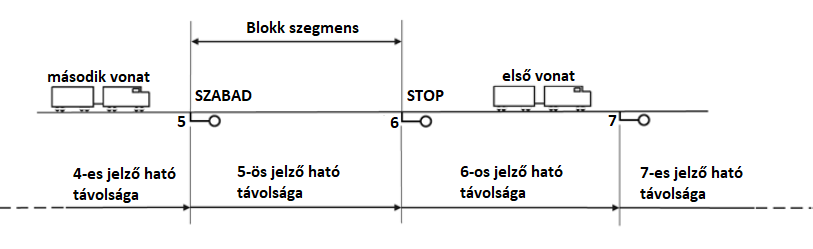
\includegraphics[width=\linewidth]{images/automatic_block.png}
	\caption[Automata blokk]{Egyszerű automata blokk elvi rajza}
	\label{fig:automatic_block}
\end{figure}

Az alap elv az hogy a vonal szegmenseket alrészekre osztjuk fel, azaz blokk egymást követő sorozatára.
Az ehhez tartozó fő szabály pedig az hogy egy blokkban egy időben csak egyetlen vonat tartózkodhat.
A blokkok közötti kommunikációt pedig a jelző hálózat biztosítja.
Tehát a blokk mind két végén kell lennie egy jelző készüléknek amelyek aspektusa módosul amint a vonat elérte ezt a pontot.
Valamint a blokkban kell lennie egy észlelő készüléknek amely garantálni tudja azt hogy egy jármű elhagyta a blokkot.
Továbbá a mérete akkorra kell legyen hogy \textit{STOP} aspektussal találkozva a vonatnak létezzen egy biztonságos megállási távolság.


A blokk elv viszonylag régi múltra tekint vissza, és tág értelemben kronológiailag a következő típusai léteznek:
\begin{enumerate}
	\item \textbf{Kézi blokk}\\
	Ez volt a kezdeti formája, konkrétan a vezető amint elért egy jelző készüléket a vonalon manuálisan kellet beállítsa a készüléket ahhoz hogy a következő érkező vonat tudja hogy foglalt a következő blokk.
	Emellett különböző folyamatokkal értesítették(pl. telefon segítségével) egymást és az operátort a blokk állapotáról, de első sorban a menetrend alapján váltogatták a jelzők aspektusát.
	Ez ahhoz vezettet hogy ha valamelyik vonat valamilyen okból kifolyólag késet, akkor az összes követő vonat is késést szenvedett. Ez egy nagyon nem hatékony hálózat kihasználtsághoz vezet.
	Pár helyen napjainkban is alkalmazzák ezt az elvet, viszont a következő elv kifejlesztésének következménye képen elavulóban van.
	Ennek megfelelője az ETCS 0 szint amely többnyire látás alapú behatolást engedélyez ehhez hasonló pályákon.
	\item \textbf{Automatikus blokk}\\
	Két tényező váltotta ki az automatikus blokk kifejlesztését és tág körű használatát.
	Az első az volt hogy, a késés tényezőn kívül, a kézi blokk rengeteg emberi erőforrást igényelt, és ebből következően több emberi hibához is vezethetett, ami amint eddig is láthattuk katasztrofális következményekkel járhat.
	A másik pedig a technológia fejlődése, és a modern észlelő rendszerek, meg jelzők, megjelenése volt.
	Kikerülve a kézi megoldást, így nagyon felgyorsul az egymást követő vonatok gyakorisága. Ami a hálózat magasabb szintű kihasználásához, valamint a vonatok gyakrabb és pontosabb menetrendjéhez vezet.
	Tehát ez az elv bevezetése költségek csökkentését és a vasút hálózat kapacitásának a megnövelését eredményezte. 
	Legtöbb automata blokk rendszer, három vagy négy blokkos lefedést alkalmaz. Tehát ha egy jármű található az első blokkban akkor a biztosító rendszer automatikusan megtiltja a behajtást, valamint figyelmeztető jelzést állít be a második blokkban.
	Végül a harmadik blokkban normális behajtást engedélyez. Ez e lefedés sűrűn átjárt hálózatok esetén állhat négy vagy több blokkból, megnövelve a biztonsági tényezőt.
	Megfelelője részleg az ETCS 1-2 szintje.
	\item \textbf{Mozgó blokk}\\
	A mozgó blokk gyakorlatilag tükrözi az egész elvet. A blokk már nem egy pálya szegmenst képvisel, hanem minden vonat kibővítve egy biztonsági távolsággal előtte és mögötte, képez egy blokkot.
	Tovább lépve szükséges tudni a hálózatban az összes vonat helyzetét és sebességét, valamint mindegyik folytonos kommunikációs kapcsolatban kell legyen egy központi vezérlő fennhatósággal.
	Ez az elv alapján lehetne maximalizálni a hálózat kapacitást. Mivel így a vonatok a lehető legközelebb tudnak egymáshoz képest átjárni a hálózaton, betartva a biztonsági protokollokat.
	Ennek a teljes megfelelője az ETCS 3-as szint, amely napjainkban még fejlesztés alatt áll. Közjáratokon még nincs implementálva ehhez hasonló rendszer.	
\end{enumerate}

Összegezve elmondható hogy napjaikban az automata blokk elv örvend a legnagyobb népszerűségnek. 
Amely az alkomponenseket egy blokkba zárva automatikusan meghatározza a vonat hálózat blokkjaiban a behajtási engedélyt.
Továbbá az automata blokk egyirányú mozgást feltételez.


\newpage
%3
\section{Elméleti megalapozás}\sectionro{Baze teoretice}\label{theory_section}

\subsection{Pequetren vasút modell}\subsectionro{Model de cale ferată Pequetren} \label{sec:ptmodell}
A tervezett vasúti rendszer kiinduló pontját képzi a \textit{Pequetren} gyártó \textbf{J34167} azonosítóval rendelkező terméke [\ref{fig:peque_tren}].
Ez egy, a vasút modell gyártók standard skálái szerint, HO kategóriás modell.
A HO kategória számszerűen 1:87-es skálázást jelent.

\begin{figure}[htp]
	\centering
	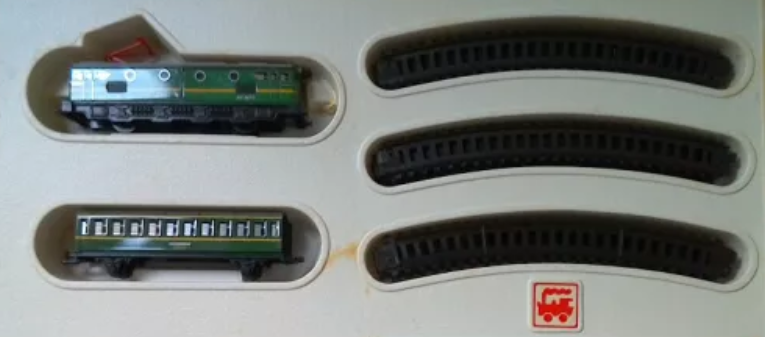
\includegraphics[width=\linewidth]{images/peque_tren.png}
	\caption[Vasút modell]{A modell, amelyre a rendszerünk épül}
	\label{fig:peque_tren}
\end{figure}

Ez a termék egy mozdony és vágányokat tartalmazz.
Pontosabban 12 darab, egyenként 24 centiméter hosszú és 1,6 centiméter szélles, enyhén görbíttet vágányt. 
Vagyis egy 2,9 méter hosszú kör alakú pálya megépítésére alkalmas.


A jármű pedig egy 16 centiméter hosszú mozdony. 
Ez a mozdony gyári előírás szerint egy 3 Voltos elem telepet igényel a meghajtáshoz.
A működésben hozása nagyon egyszerű, két darab 1,5 V-os elemet helyezve a kijelölt foglalatban és a rendelkezésre bocsájtott kapcsolóval zárva az egyszerű áramkört, a motor folyamatosan hajtja a kerekeket.
Pontosabban egy egyen áramú motor tengelye, mechanikus áttétel, hajtja a mozdony hátsó kerekeit.

Fontos megemlíteni hogy a termék semmilyen egyéb áramkörrel nem rendelkezik amely az automatizálási folyamatot segítené.

Mivel a gyártó csak ennyi információt bocsájt a rendelkezésünkre, a tervezés fejezetben bővebben kitérünk még a motor vezérlésére.

\subsection{Vezérlés - Arduino NANO}\subsectionro{Control - Arduino NANO}\label{sec:arduinonano}
Az \textbf{Arduino NANO} [\ref{fig:arduino_nano_overview}. ábra] egy olyan multifunkcionális kis méretű fejlesztői lap amely a 8 bites ATmega328P, AVR családban tartozó, mikróvezérlő körül épül.
Sajátos tervezése és méretének köszönhetően, viszonylag egyszerűen beépíthető legtöbb mikróvezérlő centrikus projektben.

\begin{figure}[htp]
    \centering
    \begin{minipage}{0.45\textwidth}
        \centering
        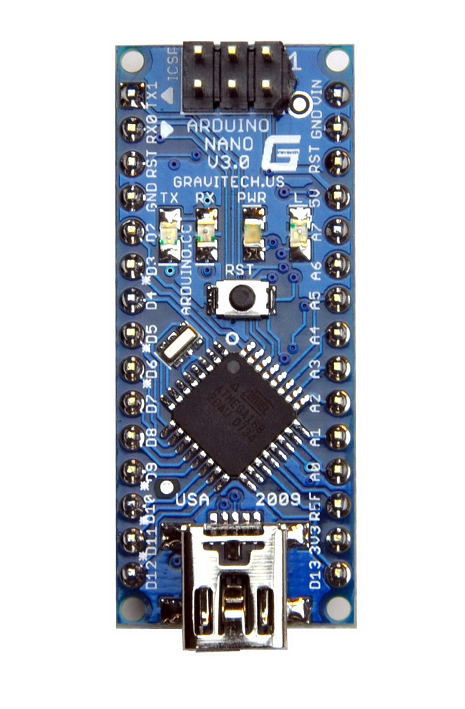
\includegraphics[width=0.7\textwidth]{images/arduino_nano_overview.png}
        \caption[Arduino Nano felülnézet]{Arduino Nano felülnézet}
		\label{fig:arduino_nano_overview}
    \end{minipage}\hfill
    \begin{minipage}{0.45\textwidth}
        \centering
        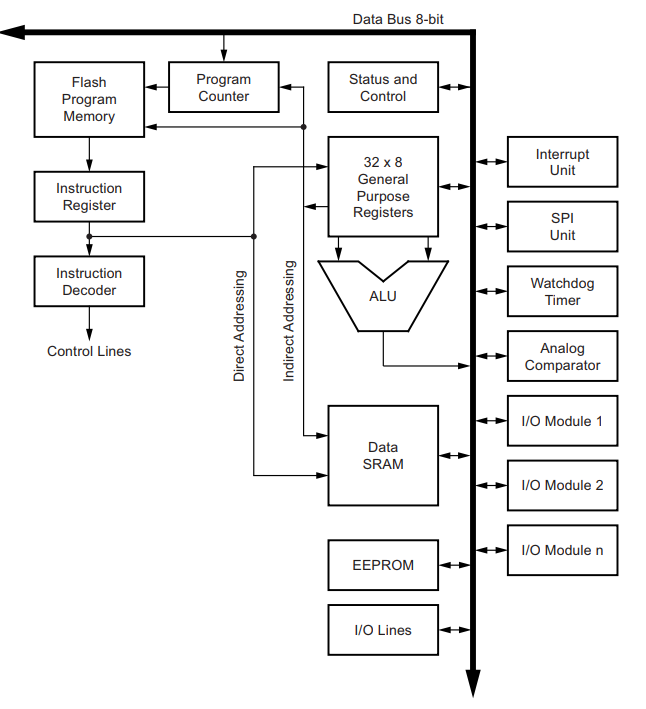
\includegraphics[width=0.9\textwidth]{images/atmega328P_block_diagram.png}
        \caption[ATmega328P blokk diagram]{ATmega328P blokk diagram}
		\label{fig:atmega328P_block_diagram}
    \end{minipage}
\end{figure}

\subsubsection{ATmega328P MCU struktúrája}\subsubsectionro{Structura MCU-ului ATmega328P}

Az \textbf{ATmega328P} egy kis fogyasztású, 8 bit-es, CMOS mikróvezérlő. 
A mikróvezérlő az AVR gyártó által fejlesztett RISC architektúrájára  épül \textbf{Reduced Instruction Set Computer}. 
Maga a RISC architektúra a Harvard architektúra leszármazottja.
Ennek az elve lényegében az hogy a mikroprocesszor egy kis méretű, nagyon optimizált, utasítás készletet használ.
Ezen architektúra alternatívája az úgy nevezett von Neumann architektúra, amely komplex utasítás készletet használ.
Annak ellenére hogy a RISC alapján több utasítást kell a processzor elvégezzen, ezek végrehajtása csak egy órajelnyi időt igényelnek. 
A "redukált utasítás készlet" pedig kevesebb tranzisztor igényel a tároló helyen (CISC-hez képest) így több hely marad általános célú regisztereknek. \cite{er00}
Felbontva kisebb utasításokra a munkát a tároló regisztereket nem szükséges kitörölni, mint a CISC-nél.
A jól meghatározott teljesítmény egyenlet alapján látható, hogy míg a CISC megközelítés az \textit{utasítás} paramétert, addig a RISC a \textit{ciklust}, pontosabban a \textit{ciklus/utasítás} csökkentésével éri el ugyanazt az eredményt:
\begin{equation*}
\frac{\text{idő}}{program} = \frac{\text{idő}}{ciklus} \times \frac{ciklus}{\text{utasítás}} \times \frac{\text{utasítás}}{program}
\end{equation*}
A \ref{fig:atmega328P_block_diagram}. ábrán bemutatott ATmega328P blokk diagramján láthatjuk a RISC architektúra alapú mikróvezérlő blokk diagramját.
A mikróvezérlő adatlapjából pedig a következő képességeket olvashatjuk ki \cite{avratm15}.
Az aritmetikai logikai egység \textbf{(en: ALU) }végzi el az utasításokat, betöltve a 32x8-as regiszterekben az operáció bemeneteit valamint eredményeit.
Az ATmega328P 131 utasítást tartalmazz az utasítás regiszterben. Egy 16 MHz-es oszcillátor kristály biztosítja a másodpercenkénti óraciklus gyakoriságát.
Az írt programot feltölthetjük a 32 KByte-os flash memóriában. Továbbá belső használatra tartalmazz 1 KByte EEPROM, valamint 2 KByte SRAM memóriát.
Végül pedig egy szélles skálájú periferikus funkciókkal rendelkezik:

\begin{itemize}
	\item Két 8 valamint egy 16 bites időzítő/számláló
	\item 6 PWM csatorna
	\item 8 10 bites ADC csatorna
	\item Programozható soros USART interfész
	\item Mester/szolga soros SPI interfész
	\item I2C interfész
	\item Analóg komparátor
	\item Megszakítási és felébresztő bemenetek
\end{itemize}

Mivel a fejlesztő lapnak köszönhetően a felprogramozás, regiszterek kezelése, valamint időzítés automatikusan kezelve van, ennél bővebben nem szükséges az mikróvezérlő működését tanulmányozni.
A többi használt funkcionalitást pedig a következő fejezetben részletezzük.

\subsubsection{Arduino NANO funkciói}\subsubsectionro{Funcțiile al Arduino NANO}
Az Arduino fejlesztő lapok az \textit{arduino.cc} vállalkozás nyílt forráskódú szoftver és hardver terméke.
Egyszerűsített félépítése és programozhatósága miatt rendkívüli népszerűségnek örvend.
A Nano az egyik legkisebb méretű ilyen fejlesztő lap, amelynek a központjában a korábban említett ATmega328P mikróvezérlő áll.
A mikróvezérlőt kibővítettek még pár funkcionalitással amely megkönnyíti akár a hétköznapi felhasználó számára is a használatot.
Ennek ellenére a nagyon kompetens mikróvezérlőnek köszönhetően a legtöbb beágyazott vagy IOT rendszer központi pillére lehet.

\begin{table}[!htbp]
    \centering
    \begin{tabular}{|c|c|c|}\hline
        Kivezetés szám & Fő szerep & Másodlagos szerep\\ \hline
        D0 - D13 & Digitális ki/be menet &  \\ \hline
		A0 - A7 & Analóg be menet & Digitális ki/be menet \\ \hline
        D0 (RX) és D1 (TX)  & & Soros kommunikáció \\ \hline
        D3, D5, D6, D9, D11 & & PWM képes \\ \hline
		A4, A5 &  & I2C kommunikáció \\ \hline
		D10, D11, D12, D13 &  & SPI kommunikáció \\ \hline
		D13 &  & Állapot led\\ \hline
		D2, D3 &  & Külső megszakítás \\ \hline
    \end{tabular}
    \caption[Arduino Nano pin beosztás]{Arduino Nano kivezetés beosztás}
    \label{tab:arduino_pint_out}
\end{table}

A \ref{tab:arduino_pint_out}. táblázatban található kivezetés beosztáshoz, láthatóan több funkció is tartozhat \cite{adaq18}:

\begin{itemize}
	\item \textbf{Digitális ki/be menet}
	Alapvetően ebben a módban a kivezetés digitális logikai igen vagy nemet olvas vagy ír.
	Azaz \textit{+5V } az a logika IGEN (\textbf{HIGH}) és a \textit{0V} a logikai nem (\textbf{LOW}).
	\item \textbf{Analóg be menet}
	Ezek a bemenetek képesek \textit{0V - 5V} tartományban észlelni feszültséget.
	Az így beolvasott értéket egy ADC áramkör átalakítja digitálisan értelmezhető jelre.
	Az Arduinoban található ADC 10 bites felbontásra képes. 
	Ez az jelenti hogy az említett feszültség intervallumot $2^{10} = 1024$ részre ossza fel, arányosan az észlelt feszültséggel.
	Operációs módtól függően az analóg bemenetek konfigurálhatóak digitális ki/be menetekként is.
	\item \textbf{Soros kommunikáció}
	A fejlesztőlap a D0 és D1 kivezetések segítségével képes soros kommunikációt megvalósítani más mikróvezérlőkkel vagy más soros kommunikációra képes készülékkel, pl. számítógép.
	Az Arduino NANO esetében ez a két port egy B típusú mini USB porta van bekötve.
	Amikor aktív a kommunikáció a D0 RX és a D1 TX módba áll.
	RX az adat fogadást képviseli(\textit{en: Receive}), TX pedig az adat küldést (\textit{en: Transfer}).
	Ezt a kommunikációt az ATmega328P USART (\textit{en: Universal Synchronous/Asynchronous Receiver/Transmitter}) csipje valósítja meg felhasználva a standard RS-232C kommunikációs protokollt.
	Ebből következően a kommunikáció létrehozható szinkron és aszinkron módban is. 
	Röviden szinkron módban nagyobb adatmennyiséget tudunk egyidőben továbbítani több sorosan csatlakozott készüléknek.	
	\item \textbf{Impulzus szélesség moduláció képes}
	A D3, D5, D6, D9 és D11 portok PWM képesek. Ez azt jelenti hogy képesek digitális jeleket analóg formában önteni.
	A PWM egy modulációs technika amelynek két fontos paramétere van: az aktív ciklus idő és a frekvencia.
	A frekvencia megadja hogy mennyi idő szükséges egy ciklus teljes befejezéséhez, és hogy milyen gyorsan vált a digitális jel a HIGH és LOW értékek között.
	Az aktív ciklus idő legtöbbször százalékosan van jelenítve. A lap egy 8 bites PWM kimenetre képes, tehát $2^{8} = 256$ felbontásban tudjuk ezt irányítani.
	Konkréten ha az aktív ciklus 100(\%) akkor a kimeneten folytonos 5V fog megjelenni, ezt ha csökkentjük például 75(\%)-ra akkor $5V \times 0.75 = 3,75 V$-t tudunk kialakítani.
	\item \textbf{$I^{2}C$ kommunikáció}
	Az A4 és A5 port másodlagos szerepében az $I^{2}C$ kommunikációra képes. 
	Ez egy szinkron multi-mester multi-szolga kapcsolatot képes létrehozni ugyancsak soros kapcsolatra épülve.
	\item \textbf{SPI kommunikáció}
	Soros periféria interfészt használva egy következő szenzorlapot vagy mikróvezérlőt köthetünk össze a saját lapunkkal. 
	A létrejött kapcsolat ugyancsak egy soros kommunikációt valósít meg, egy mester- egy vagy több szolga adat buszt képezve.
	Itt az említett portoknak fontos szerepe van amelyet nem lehet figyelmen kívül hagyni konfiguráció közben:
		\begin{itemize}
			\item D10 - \textit{SS - Slave Select}
			Meghatározza hogy a mester melyik szolga készülékkel kommunikáljon.
			\item D11 - \textit{MOSI - Master Out Slave In}
			A mester adat vonala, amelyen küldi az adatot a periferikus szolgának.
			\item D12 - \textit{MISO - Master In Slave Out}
			A szolgák adat vonala, amelyen adatot küldhetnek a mesternek.
			\item D13 - \textit{SCK - Serial Clock}
			A mester által generált óra jel, az adat továbbítás szinkronizációja miatt szükséges.
		\end{itemize}
	\item \textbf{Állapot led}
	Ez egy beépített piros színű miniatűr led, szabadon használható a felhasználó által.
	\item \textbf{Külső megszakítás}
	A D2 és D3 portok INT0 valamint INT1 funkciója biztosítja a külső megszakítást. 
	Erre legtöbbször akkor van szükség amikor valamely kritikus esemény miatt szükséges a mikróvezérlő aktuális feladatát megszakítani, ahhoz hogy figyelmét erre az eseményre fordítsa.
\end{itemize}

Az említett komponenseken kívül a fejlesztő lapon találhatunk még egy B típusú USB portot. 
Ha nem használjuk az USB portot, a táplálást egy külső forrásból is megoldhatjuk a $V_{in}$ és GND portokat használva.
A készülék a 7-12V-os feszültség intervallumban szükséges táplálni.
Továbbá még található egy 5.5V, egy 3.3V-os és még egy GND port amelyek egyéb periferikus áramkörök meghajtására is alkalmasak lehetnek.

\subsubsection{Arduino programozása - Arduino IDE}\subsubsectionro{Programarea Arduino-ului - Arduino IDE }
A fejlesztő lap programozása automatizálva van \cite{ardtut19}. 
A felhasználónak nem szükséges a sokszor körülményes mikróvezérlő felprogramozástól megijednie.
Az Arduino saját fejlesztő környezete az \textbf{Arduino IDE} és a fejlesztőlapra előre megírt boot-loader segítségével ez a folyamat pár egyszerű lépésre redukálódott.
A folyamat a következő egyszerű lépésekre bontható:
\begin{enumerate}
	\item Arduino IDE telepítése a saját számítógépre
	\item Az Arduino driver telepítése az operációs rendszerre
	\item A fejlesztő lap összekötése USB porton keresztül a számítógéppel
	\item Az operációs rendszer port listájában megjelenik egy sajátos azonosítóval a készülék, pl. \textit{COM2}	
	\item A fejlesztő környezet élindítása
	\item A \textit{Tools - Boards} menülistában a fejlesztőlap típusának kiválasztása, pl. \textit{Arduino Nano}
	\item A \textit{Tools - Port} menülistában a helyes port kiválasztása pl. \textit{ez esetben COM2}
	\item A program megírása
	\item A kód kompilálása
	\item A kód feltöltése a fejlesztőlapra
\end{enumerate}

A többi beállításon legtöbbször nem szükséges módosítani.
A fejlesztő környezet igényeli a \textit{C} programozási nyelv ismeretét.
A környezet egy egyszerű két függvényes program implementációt használ:



\begin{lstlisting}[style=CStyle, caption={A \mintinline{cpp}{setup()} és a \mintinline{cpp}{loop()} függvény Arduino IDE-ben },label=fig:arduino_ide_code_eg]
// setup runs once at start or at reset of board
void setup(){
  pinMode(LED_BUILTIN, OUTPUT);
}
// loop repeats itself infintely
void loop() {
  digitalWrite(LED_BUILTIN, HIGH);
  delay(1000);
  digitalWrite(LED_BUILTIN, LOW);
  delay(1000);
}
\end{lstlisting}



A fenti program, a beépített LEDet villogtatja 1 másodpercenként.
A program két jól elkülöníthető részre osztható. 
A \mintinline{cpp}{setup()} függvény a portok és egyéb perifériák iniciálására szolgál. 
Valamint ide írható az összes olyan logika amely induláskor egyszer kell hogy lefusson.
A \mintinline{cpp}{loop()} függvény pedig végtelen ciklus szerűen ismétlődik. 
Az itt található kód összeköthető a belső óra jellel, egy üres \mintinline{cpp}{loop()} függvény például 10 KHz-es frekvenciával fog ismétlődni.
Ez a kód résznek kell tartalmaznia azt a logikát amely megvalósítja a normál működésben elvárt célt.

\subsection{Rádió frekvenciás kommunikáció}\subsectionro{Comunicare pe frecvențe radio}\label{sec:rftcomm}
\subsubsection{NRFL24 rádió frekvencia kommunikációs modul}\subsubsectionro{NRFL24 modul de comunicare pe frecvențe radio}

\begin{wrapfigure}{l}{0.40\textwidth}
	\vspace{-20pt}
    \centering
    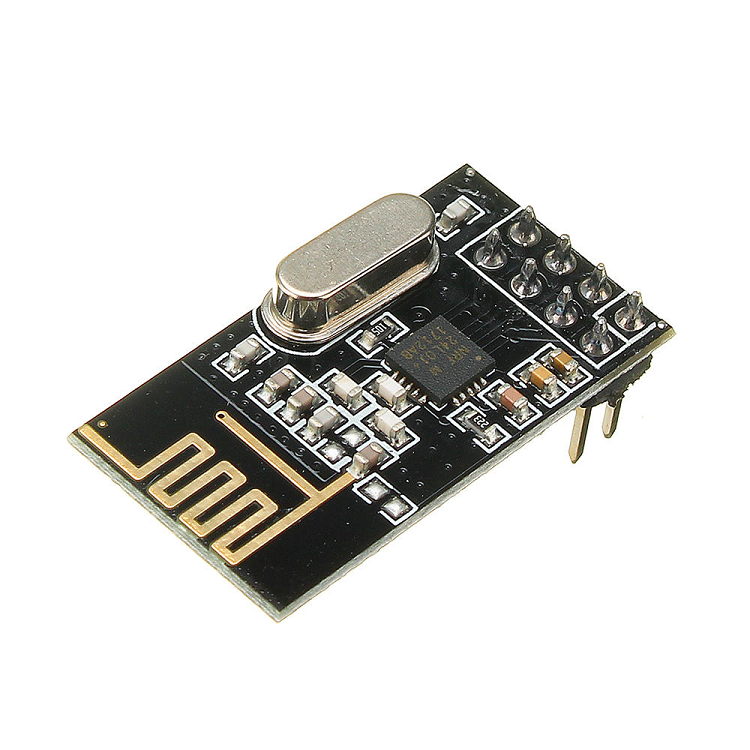
\includegraphics[scale=0.25]{images/nrf24l01_overview.png}
    \caption[nrf24l01 felülnézet]{nrf24l01 felülnézete}
    \label{fig:nrf24l01overview}
\end{wrapfigure}

Az NRFL24 egy egy csipes rádió adó-vevő készülék. \cite{nosem06}
A világszerte használt 2,4-2,5 GHz-es ISM sávot használja kommunikációs csatornaként.
A főbb képességeit érintve SPI soros kommunikáció segítségével vezérelhető.
1-2 Mbps sebbegésekre képes a levegőn keresztül.
125 rádió frekvenciás csatornán működik.
Nagyon kis mérete és nagyon kis fogyasztása alkalmassá teszi a legtöbb kábel nélküli készülék fejlesztésére.
8 portos kivezetése van amelyek a következőek: 3.3V, GND, CE, CSN, MOSI, SCK, MISO, IRQ.
Amint látható SPI kommunikáció kompatibilis, a már korábban leírt SPI kommunikáció seftiségével könnyen csatlakoztatható az Arduino Nano SPI képes portjaira.
A CE - \textit{Chip Enable} port segítségével aktiváljuk az SPI kommunikációt.
Valamint a CSN - \textit{Chip Select Not} port szerepe hogy életben tartsa ezt.
A 3.3V-os és GND port a táplálásra szolgál. Míg a többi port az SPI kommunikáció alfejezetben leírt feladatokat látja el.

\subsubsection{NRFL24 hálózatok és kommunikációs protokoll}\subsubsectionro{Rețele de NRFL24 și protocol de comunicare}\label{sec:nrlf24rfc}

A \ref{fig:nrf24l01_network}. ábra jelképezi ennek a rádió adó-vevőnek a másik fontos képességét.

\begin{figure}[htp]
	\centering
	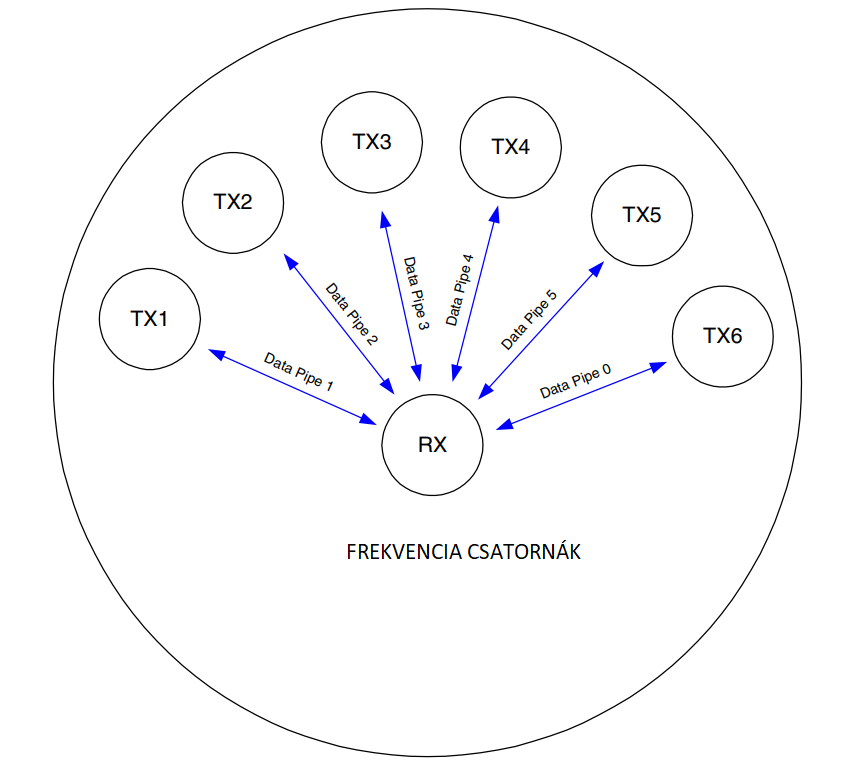
\includegraphics[scale = 0.6]{images/nrf24l01_network.png}
	\caption[nrf24l01 network]{nrf24l01 hálózati kommunikáció mester-szolga módban}
	\label{fig:nrf24l01_network}
\end{figure}

Egyszerű módon lehet ugyan ilyen típusú modulok között kábel nélküli hálózatot kialakítani.
Egy nrf24l01 modul, mester-szolga kapcsolatot létrehozva, egészen 6 darab másik modullal képes digitális adatcsövet fenntartani.
Fontos viszont egyedi címet meghatározni mindegyik modulnak. Hogy a hálózati kommunikáció során tudják azonosítani egymást.
Tovább lépve a fenti példában említett szolgákhoz további 5 modult lehet csatlakoztatni. 
Akik a szolgák szolgái lennének. Ilyen módon 5 szintes mélységig lehet bővíteni a hálózat, elméletileg 3125 modul a fizikai határ.
Ez roppant értékes skálázási szemszögből. Maga a hálózat felépítését bináris fa topológiaként lehet elképzelni.
Adott a mester modul aki az alapot jelképezi, lefele haladva a fán pedig, lehet 5 gyereke, akiknek megint lehet 5 gyereke, stb.

\subsection{74HC595 léptető regiszter}\subsectionro{Registru de deplasare 74HC595}\label{sec:shiftregister}

\begin{wrapfigure}{l}{0.40\textwidth}
	\vspace{-20pt}
    \centering
    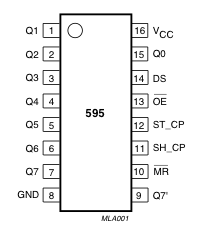
\includegraphics[scale=1]{images/74HC595_pinlayout.png}
    \caption[74HC595 portjai]{74HC595 portjai}
    \label{fig:shiftregister}
\end{wrapfigure}

Sok esetben fordulhat elő, hogy a mikróvezérlőnk digitális kimenetei nem elégségesek az alkalmazásunk összes komponensének a vezérlésére.
Ilyen esetben használunk léptető regisztereket. Egy ilyen alkatrész a 74HC595 léptető regiszter.
Ez egy 8 bites soros-be vagy párhuzamos-ki adatátvitelt biztosít.
Működése a szinkron soros kommunikációra épül.
Röviden mindegyik ciklus órajelre a kívánt adatokat betöltjük bitenként a regiszterbe. 
Miután a teljes byte-nyi adat betöltésre került, a regiszter az egyéni portjain mindegyik biten található \textit{HIGH} vagy \textit{LOW} értéket egyéni portokon továbbítja a vezérelendő komponensekre.
Látható hogy sorosan töltjük be, és párhuzamosan küldjük ki az adatokat. 
Mivel egy óra jelnyi ciklus, nagyon rövid idő (mikró másodpercnyi érték), nem észrevehető az az elvesztett idő amíg 1 Byte betöltődik a regiszterben.
A regiszternek van egy soros kimenet portja is, amely segítségével több regisztert is sorba köthetünk.
Igy egy ciklusban az érkező adat nem csak az aktuális, ha nem a következő regiszter soros bemenetén is megjelenik az adat. Ezt nevezzük léptető regiszterek láncba kötésének.
A \cite{tein19}. forrásban leírt adatlap alapján láthatjuk a \ref{fig:shiftregister}. ábrán a  szilikon csip port elhelyezéseit valamint az \ref{tab:shiftregister}. táblázatban ezek jelentéseit.

\begin{table}[!htbp]
    \centering
    \begin{tabular}{|c|c|} \hline
        Port azonosító & Megnevezés \\ \hline
        $Q_{0} - Q_{7}$ & Párhuzamos kimeneti portok \\ \hline
        GND & Föld  \\ \hline
        $Q_{7'}$ & Soros kimenet \\ \hline
        MR & Mester vissza állítás \\ \hline
        SH\_CP & Regiszter órajel port \\ \hline
        ST\_CP & Regiszter puffer órajel port \\ \hline
        OE & Kimenet aktiválás \\ \hline
        DS & Soros adat bemenetel \\ \hline
        $V_{cc}$ & Táp \\ \hline
    \end{tabular}
    \caption[74HC595 port leírás]{74HC595 léptető regiszter port magyarázat}
    \label{tab:shiftregister}
\end{table}


\subsection{Fotó ellenállás}\subsectionro{Fotorezistoare}

\begin{figure}[htp]
    \centering
    \begin{minipage}{0.45\textwidth}
        \centering
        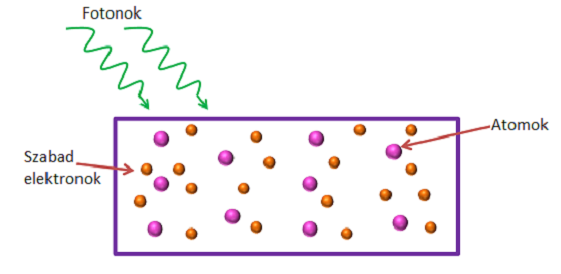
\includegraphics[width=\textwidth]{images/ldr_principle.png}
        \caption[LDR elv]{Fotó ellenállás elvi működés}
		\label{fig:ldr_principle}
    \end{minipage}\hfill
    \begin{minipage}{0.45\textwidth}
        \centering
        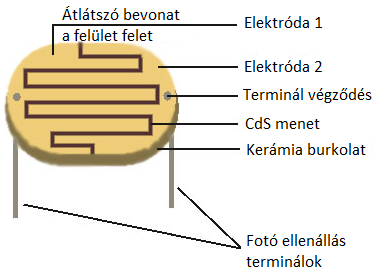
\includegraphics[width=0.75\textwidth]{images/ldr_structure.png}
        \caption[LDR struktúra]{Fotó ellenállás felépítése}
		\label{fig:ldr_structure}
    \end{minipage}
\end{figure}

A fotó ellenállás egy egyszerű szenzor. 
Amint a neve is elárulja, lényegében egy olyan elektronikus érzékelő amely fény hatására változtatja ohmikus ellenállását.
Félvezetőként működik, az az külső hatásra, ez esetben fotonok, a CdS (Kadmium szulfit) menetben az atom szintű kötések megbomlanak (\ref{fig:ldr_principle}. ábra).
Ennek következménye képen elektron lyukak és szabad elektronok jelenek meg, és szabad mozgásra képesek az anyagon belül.
A fény hatására a töltés hordozok száma növekszik, tehát az átfolyó áram erőssége is növekszik. 
Áram erősség növekedésének direkt hatása az ellenállás csökkenése. Tehát lényegében a fény erősség növekedése ellenállás csökkenéséhez vezet.
A szakterületen egy gyakori implementációja ennek az elvnek a PGM5516 kóddal ellátott fotó-ellenállás (\ref{fig:ldr_structure}. ábra), amelyet a Token Electronic \cite{toel19} gyártja, és technikai paramétereit a \ref{ldrparams}. táblázatban foglaltuk össze:

\begin{table}[!htbp]
    \centering
    \begin{tabular}{|c|c|c|c|c|c|}\hline
        \specialcell{$V_{max}$\\(VDC)} & 
        \specialcell{$P_{max}$\\(mW)} & 
        \specialcell{Spektrális csúcs\\(nm)} & 
        \specialcell{Ohmikus R\\($k\Omega$)} & 
        \specialcell{Sötétben R\\($M\Omega$)} & 
        \specialcell{Reszponzív idő \\(ms)} \\ \hline
        100 & 90 & 540 &  $2\sim6$ & 0.15  & $30\sim40$  \\ \hline
    \end{tabular}
    \caption[LDR paraméterek]{Fotó ellenállás paraméterei}
    \label{ldrparams}
\end{table}

\subsection{Egyéb szoftverek}\subsectionro{Alte software-uri}
\subsubsection{Fritzing áramkör tervező}\subsubsectionro{Fritzing software de circuit design}
A Fritzing egy nyílt forrás kódú, egyszerűségre törekvő, automatizált áramkör tervező szoftver.
Széles körű adatbázisában a legtöbb elektronikai komponens megtalálható. Továbbá lehetőséget add tesztpanel de nyomtatott áramkör tervezésre is. Mivel egy nyílt forrás kódú termék, a fejlesztése a közösség által történik, és rengeteg anyagot bocsájtanak a felhasználok rendelkezésére \cite{frifo19}.
\subsubsection{Processing UI dizájner}\subsubsectionro{Processing UI designer}
A Processing egy rugalmas, a Java programozási nyelvre alapuló, grafikus interfész vázlatát és kódját implementáló keretrendszer.
Egyszerű megközelítése a kellemes felhasználói felületek készítésére hasonlít az Arduino IDE implementációjára.
Ez is egy függvény orientált környezett, az az a programozó rendelkezésére áll két fő függvény, amelyekben a logika nagy része implementálható.
Természetesen további függvények létrehozhatóak, valamint külső csomagokban osztályok is. Viszont az összes példányosításra, vagy felhívásra, kell hogy kerüljön ebben a két függvényben. 
Ez a két függvény a \mintinline{java}{setup()} és a \mintinline{java}{draw()} függvények. 
Hasonlóan mint az Arduino IDE, itt is az első az inicializálásért, a második pedig a ciklikusan ismétlődő kód futtatásáért fellelős. Mivel egy nyílt forrás kódú termék, a fejlesztése a közösség által történik, és rengeteg anyagot bocsájtanak a felhasználok rendelkezésére \cite{profo19}.

\subsubsection{\LaTeX,  dokumentum szerkesztő}\subsubsectionro{Latex editor de text}
A \LaTeX, egy ingyenes, magas minőségű szöveg szerkesztő és formázó rendszer.
Parancsok által olyan funkciókat tartalmaz, amelyek technikai és tudományos dokumentumok készítésére alkalmas.
A tudományos körökben standard módon elfogadott a publikálandó dokumentumok ebben a rendszerben való készítése.
Mivel egy nyílt forrás kódú termék, a fejlesztése a közösség által történik, és rengeteg anyagot bocsájtanak a felhasználok rendelkezésére \cite{latpro19}.

\newpage
%4
\section{A rendszer célja}\sectionro{Scopul sistemului}
A dolgozat célja egy olyan vasút modell hálózat készítése amely a valóságban található vasút hálózatok működését tükrözi.
Ezt a tanulmányozott ETCS elvek alapján valósítjuk meg, és a következő  alrészekre osztottam, tematika szerint:
\begin{itemize}
	\item \textbf{Mechanikus}: A modell vasút kiegészítő komponensei, amelyek nem a direkt funkcionális működéshez szükségesek. Pl: a vágányokat, jelzőket tartó mechanikus platformok.
	\item \textbf{Hardver}: Azok az elektronikus komponensek összessége, amelyek a mechanikus részre épülve, megvalósítják az architektúra és specifikáció által előírt gépi feladatokat.
	\item \textbf{Szoftver}: Azoknak a programoknak az összessége, amelyek a hardveri komponenseket vezérlik, és elvégzik a rendszer logikai funkcióit.
\end{itemize}

A projekt kivitelezésében alkalmaztam a \ref{cenelecchapter}. fejezetben tanulmányozott V modell (\ref{fig:cenelec_vmodel}. ábra) egyszerűsített változatát. 
Ez alapján történt a követelmények és specifikációk meghatározása, valamint a tényleges megvalósítás is. 
%5
\section{Rendszer követelményei}\sectionro{Cerințele sistemului}
A megvalósítandó rendszer követelményei válaszolnak a \textit{Mit szeretnénk megvalósítani?} kérdésre. A \ref{RAbasics}. fejezetben megismert elvek és a \ref{sec:ptmodell}. fejezetben leírt modell, valamint a korábban említett felosztás alapján a következő táblázatokban (\ref{tab:mechrequirment}, \ref{tab:hardrequirment}, \ref{tab:softrequirment}) szögeztem le mindegyik alrész követelményeit:

\begin{table}[!htbp]
    \centering
    \begin{tabular}{|c|m{12cm}|} \hline
        Nr. & Elvárt mechanikus követelmény\\ \hline
        1 & \specialcell{A vasút vágányokból felépített vágány hálózatnak egy stabil, \\hordozható platform} \\ \hline
        2 & \specialcell{A jelző hálózatot felépítő jelző moduloknak egy mechanikus keret \\ amely biztosítja ezek láthatóságát} \\ \hline
        3 & \specialcell{Az észlelő hálózat, észlelő moduljainak szükséges platform amely \\ az észlelést valamint ennek jelzését megvalósítja} \\ \hline
    \end{tabular}
    \caption[Mechanikai követelmény]{A rendszer mechanikai követelményei}
    \label{tab:mechrequirment}
\end{table}

\begin{table}[!htbp]
    \centering
    \begin{tabular}{|c|m{12cm}|} \hline
        Nr. & Elvárt hardver követelmény\\ \hline
        1 & Mozdony távirányított képességét biztosító hardver \\ \hline
        2 & A mozdony sebességét szabályzó hardver \\ \hline
        3 & A mozdony helyzetét jelző hardver \\ \hline
		4 & Észlelő készülék és hálózat hardver implementáció \\ \hline
		5 & Jelző készülék és hálózat hardver implementáció \\ \hline
		6 & Központi vezérlő rendszer hardver implementáció \\ \hline
		7 & Biztosító rendszer hardver implementáció \\ \hline
		8 & Rendszerek közötti kommunikációt megvalósító hardver\\ \hline
    \end{tabular}
    \caption[Hardver követelmény]{A rendszer hardver követelményei}
    \label{tab:hardrequirment}
\end{table}

\begin{table}[!htbp]
    \centering
    \begin{tabular}{|c|m{12cm}|} \hline
        Nr. & Elvárt szoftver követelmény\\ \hline
        1 & Mozdony vezérlő, hardver szintű, szoftver \\ \hline
        2 & Mozdony vezérlő, számítógépen futó, grafikus interfész \\ \hline
        3 & Észlelő hálózatot, hardver szintű, vezérlő szoftver \\ \hline
		4 & Jelző hálózatot, hardver szintű, vezérlő szoftver \\ \hline
		5 & Központi vezérlő rendszer, hardver szintű, szoftver \\ \hline
		6 & Biztosító rendszert, hardver szintű, vezérlő szoftver  \\ \hline
		7 & Vasút hálózatot követő, számítógépen futó, grafikus interfész \\ \hline
		8 & Rendszer komponensek közötti kommunikációt kezelő szoftver \\ \hline
    \end{tabular}
    \caption[Szoftver követelmény]{A rendszer szoftver követelményei}
    \label{tab:softrequirment}
\end{table}

\newpage
%6
\section{Rendszer architektúra és specifikáció}\sectionro{Arhitectura și specificațiile sistemului}
A követelmények alapján természetes módon körvonalazódik a rendszerünk architektúrája.
A fontosabb komponensek:
\begin{itemize}
	\item Mechanikus komponensek amelyek fizikai alapként szolgálnak a kész hardver rendszernek
	\item A modell mozdony automatizálása különböző hardver és szoftver funkcionalitásokkal
	\item A modell vágány menti észlelő hálózat hardver és szoftver szintű megvalósítása
	\item A modell vágány menti jelző hálózat hardver és szoftver szintű megvalósítása
	\item A rendszerek egységesítse egy központi vezérlő által, valamint a biztosító rendszer fejlesztése
	\item Egy mozdony vezérlő, valamint egy vágány hálózat figyelő grafikus interfész készítése
	\item Az említett hardver és szoftver komponensek közötti kommunikáció megoldása
\end{itemize}


\begin{figure}[htp]
	\centering
	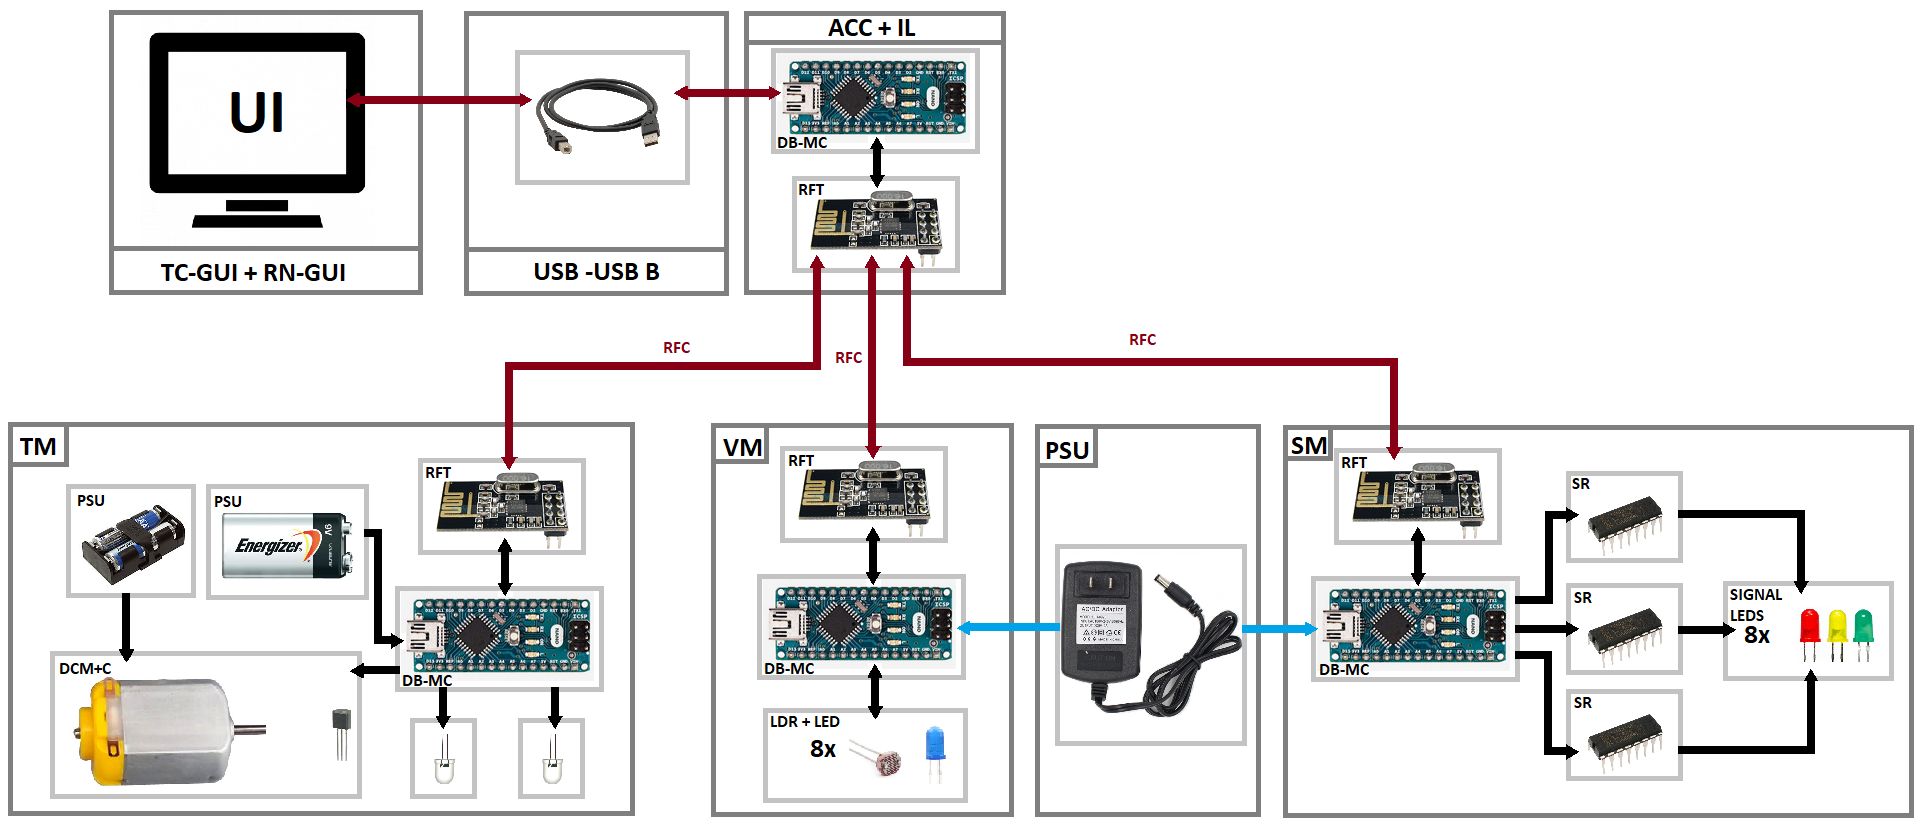
\includegraphics[width=\linewidth]{images/block_diagram_sysra.png}
	\caption[Rendszer tömbvázlat]{A modell vasút rendszer tömbvázlata }
	\label{fig:block_diagram_sysra}
\end{figure}

A tömbvázlatban használt rövidítések magyarázata a \ref{tab:specabrv}. táblázatban található.
\begin{table}[htp]
    \centering
    \begin{tabular}{|c|l|l|l|} \hline
        Nr. & Rövidítés & Angolul & Magyarázat \\ \hline
		1 & DB-MC & Dev. Board with MCU & Fejlesztőlap Mikróvezérlővel \\ \hline
		2 & RFT & Radio Frequency Transreciever & Rádió frekvenciás adó-vevő \\ \hline
		3 & LDR & Light Dependent Resistor & Fotó ellenállás \\ \hline
		4 & TM & Train Module & Mozdony modul \\ \hline
		5 & VM & Vacancy Module & Észlelő modul \\ \hline
		6 & SM & Signal Module & Jelző modul \\ \hline
		7 & ACC & Areal Central Controller & Területi központi vezérlő \\ \hline
		8 & IL & InterLocking & Óvó/Biztosító rendszer \\ \hline
		9 & TC-GUI & Train Control - GUI & Mozdony vezérlő g.i. \\ \hline
		10 & RN-GUI & Rail Network - GUI & Vágány hálózat állapot g.i. \\ \hline
		11 & PSU & Power Supply Unit & Áramszolgáltató egység \\ \hline
		12 & USB-USB B & USB to USB B channel & UI és CCM közötti soros kom. \\ \hline
		13 & SPI & Serial Peripheral Interface & Soros periféria interfész \\ \hline
		14 & RFC & Radio Frequency Channel & Rádió Frekvenciás Kanális \\ \hline
		15 & SR & Shift Register & Léptető regiszter \\ \hline
		16 & DCM+C & DC Motor + Controll & DC Motor + vezérlés \\ \hline
		17 & TIP & Train Integrity Position & Vonat teljesség helyzete \\ \hline
	\end{tabular}
    \caption[Rövidítések]{Használt rövidítések magyarázata}
    \label{tab:specabrv}
\end{table}


A \ref{RAbasics}. fejezet alapján meghatározható hogy a modell vasút hálózatra a következő ETCS ás vasúti elvek alkalmazhatóak:
\begin{itemize}
	\item ETCS 2-es szintű ATP rendszer 
	\item Zárt hálózat amely exkluzív fővágányokból épül fel
	\item A műanyagból gyártót vágányok kizárják a pályaáramkör használatát, tehát valamilyen tengelyszámláló megoldás szükséges
	\item A standard jelző aspektusok használata (\textit{piros - sárga - zöld})
	\item Óvó - Biztosító rendszer implementációja
	\item Automatikus blokk elv implementációja egy 8 blokkból álló kör szekvenciás rendszerre
\end{itemize}

Ezt leszögezve és kibővítve, a követelményekkel valamint a \ref{theory_section}. fejezetben tanulmányozott hardver és szoftver megoldássokkal a \ref{fig:block_diagram_sysra}. ábrán látható tömbvázlatot készítettem.
Továbbiakban mindegyik komponens specifikációját vázoljuk fel, a követelmények alapján.

\subsection{Mechanikus specifikációk}\subsectionro{Specificațiile mecanice}\label{sec:mechspec}
A \textbf{Pequtren} módell vasút méreteit ismerve ($L = 2,94 m$), a kör alakú zárt vágány pálya $D = 1 m$ átmérővel rendelkezik.
Ennek egy  $105 \times 105 cm$ pár milliméter vastagságú lemez alkalmas.

A jelző készüléknek szükséges egy kis felület ahova a "jelző lámpákat" rögzíthetjük, valamint a teljes készüléket, egy csavaros megoldással, a hálózat platformhoz rögzíthetjük.

Az észlelő készüléknek is egy kis felületre kell rögzítettünk az észlelő szenzort és az állapot jelző LEDet. Végül ez is egy csavaros megoldással rögzítődik a platformhoz. 

Ezeknek a mennyiségét, az architektúrában meghatározott blokkok mennyisége határozza meg, tehát 8 jelző és észlelő készülék legyártása szükséges.

\subsection{Hardver specifikációk}\subsectionro{Specificațiile hardwareului}
A hardver specifikációkat a \ref{tab:hardrequirment}. táblázatban leszögezett követelmények alapján a \ref{tab:hardspec} táblázatban foglaltam össze, használva a \ref{tab:specabrv} táblázatban definiált rövidítéseket:

\begin{table}[!htbp]
    \centering
    \begin{tabular}{|c|c|l|} \hline
        Nr. & Köv. & Megfelelő hardver specifikáció \\ \hline
        1 & 8.1 & \specialcell{A TM távirányítása ACC végzi el DB-MC, RFT+RFC és PSU (9V) 
                            \\komponensekkel valósul meg} \\ \hline
        2 & 8.2 & \specialcell{A TM sebesség szabályozását a DM-MC és egy kibővítő DCM+C, 
                            \\PSU (3V) áramkör valósítja meg}  \\ \hline
        3 & 8.3 & \specialcell{A TM a TIP funkciót fény forrás rögzítése oldja
                            \\meg, DB-MC irányítja} \\ \hline
		4 & 8.4 & \specialcell{Az VM egy LDR megoldást alkalmaz, érzékelve a 3-as specifikációban
		                    \\TIP jelet. Az automata blokkok meghatározása szerint, mind a 
		                    \\8 blokkban szükséges egy LDR áramkör. Az LDR adatok a DB-MC 
		                    \\analóg bemeneteire kapcsolódnak. Az DB-MC, PSU(9V) táplálja,
		                    \\és RFT-en keresztül továbbítja az adatokat ACC felé}\\ \hline
		5 & 8.5 & \specialcell{Az SM-t, az ACC vezéreli DB-MC, RFT + RFC és PSU (9V) 
		                    \\segítségével SM a VM által szolgáltatott adatok alapján
		                    \\számolja a szükséges jelzést. Mivel DB-MC digitális 
		                    \\kimenetei korlátozottak 3 SR állítja be a jelzést}\\ \hline
		6 & 8.6 & \specialcell{ACC RFT és RFC-n keresztül irányítja a rendszer logikát ACC 
		                    \\USB B - USB soros kapcsolatban van TC-GUI és RN-GUI-l}\\ \hline
		7 & 8.7 & \specialcell{IL az ACC szinten valósul meg, valójában hardver szintű szoftver} \\ \hline
		8 & 8.8 &\specialcell{Modulok közötti kommunikációt az RFT hálózat RFC-n keresztül 
		                    \\valósítja meg}\\ \hline
    \end{tabular}
    \caption[Hardver specifikáció]{A rendszer hardver specifikációi}
    \label{tab:hardspec}
\end{table}

\subsection{Szoftver specifikációk}\subsectionro{Specificațiile software-ului}
A szoftver specifikációkat a \ref{tab:softrequirment}. táblázatban leszögezett követelmények alapján a \ref{tab:softspec}. táblázatban foglaltam össze, használva a \ref{tab:specabrv}. táblázatban definiált rövidítéseket:

\begin{table}[!htbp]
    \resizebox{\textwidth}{!}{
    \begin{tabular}{|c|c|l|} \hline
        Nr. & Köv. & Megfelelő szoftver specifikáció \\ \hline
        1 & 9.1 & \specialcell{A TM távirányítását DB-MC-n futó szoftver hajtja végre. A végrehajtó
                            \\parancsok ACC-tol érkeznek RFC protokollal az RFT hálózaton keresztül.
							\\TM értelmezi az RFC protokollt. A TIP jelzés szoftverből 
							\\bekapcsolható. A sebesség szabályozás PWM modulációval programozható.
							\\TM továbbítja ACC-nek a sebesség aspektusát is. TM az ACC-tól érkező
							\\megállj parancsot azonnal elvégzi.} \\ \hline
        2 & 9.2 & \specialcell{A TC-GUI a parancsok elsődleges forrása. Két sebesség szint és egy 
                            \\ megállás parancsot kezdeményez. Opcionálisan jelezheti a következő
							\\ SM aspektust is.}  \\ \hline
        3 & 9.3 & \specialcell{A VM a begyűjtött LDR adatokat csomagban rendezi. A VM folytonosan 
                            \\továbbítja az aktuális csomagot ACC-nek. RFC protokollal az RFT hálózaton
							\\keresztül. A VM érzékelt bemenet esetén egy állapot jelzést aktivál.} \\ \hline
		4 & 9.4 & \specialcell{Az SM ACC-tól, RFT hálózaton érkező csomagot feldolgozza. SM is tudja  
		                    \\értelmezni az RFC protokollt. SM a megfelelő SR-ek aktiválásával vezérli 
		                    \\a jelzőket. SM folyamatosan várja az ACC-től érkező jeleket.}\\ \hline
		5 & 9.5 & \specialcell{ACC felügyelő, továbbító, vezérlő és értelmező szerepe van. ACC 
		                    \\kapcsolatban van UI komponensekkel, fogadja az innen érkező parancsokat.
							\\ACC az RFT hálózat központi komponense, RFC képes. Fogadja a VM-l
							\\értekező csomagokat. Átadja IL-nek. Fogadja a TM-töl érkező csomagot,
							\\ Átadja IL-nek. Átveszi IL-l érkező csomagot, továbbítja TM és SM-nek.}\\ \hline
		6 & 9.6 & \specialcell{IL az ACC-ben kódolt biztosító függvények összessége. IL értelmezi az 
		                    \\előkészített VM csomagot. IL értelmezi a fogadott TM információt.
							\\IL 4 blokkos jelző aspektus szekvencia algoritmust futtat. Az algoritmus
							\\kiszámolja a szükséges biztonságos aspektust a hálózat összes SM 
							\\komponensének. IL átadja a számolt eredményt ACC-nek. IL automatikusan
							\\értesíti ACC-t ha TM sebesség aspektusa nem felel meg a jelző aspektusnak.}\\ \hline
		7 & 9.7 & \specialcell{Az IL-től érkezett aspektus csomagot ACC RN-GUI-nak is továbbítja. 
							\\Valamint a figyelmeztető parancsot sebesség határ túllépése esetén 
							\\továbbítja TC-GUI-nak is.} \\ \hline
		8 & 9.8 &\specialcell{ACC és UI komponensek standard soros porton kommunikálnak. ACC,  
		                    \\VM, TM, SM egymás között, szoftverből irányítottan, az RFT 
							\\hálózaton, a fejlesztendő RFC protokollal kommunikálnak.}\\ \hline
    \end{tabular}
    }
    \caption[Szoftver specifikáció]{A rendszer szoftver specifikációi}
    \label{tab:softspec}
\end{table}




\newpage
%7
\section{Részletes tervezés és megvalósítás}\sectionro{Planificare detaliată și realizarea}
A dolgozat megvalósítása a \ref{fig:block_diagram_sysra}. ábrán bemutatott architektúra tömbvázlata, és a követelmények valamint specifikációk alapján mechanikai, hardver és szoftver alrészekre osztható.
A specifikációkban meghatározott rövidítéseket az egyszerűség kedvéért továbbra is használjuk. 
A specifikációt követve mindegyik komponens megvalósítását külön alfejezetben részletezzük.

\subsection{Mechanikai kivitelezés}\subsectionro{Implementare mecanică}
\subsubsection{Vágány hálózat platform}\subsubsectionro{Platforma pentru rețeaua de șine}
A \ref{sec:mechspec}. fejezet szerinti specifikáció alapján az első lépésben egy MDF (Medium Density fibreboard) lapot terveztem a platform elkészítéséhez.
Viszont kimérve a $1050\times1050mm$ méretű lapot, a súlya túl nagynak bizonyult. 
És mivel szempont a platform relatív mobilitása, végül egy natúr $3mm$-es vastagságú HDF-lapot választottam, amelyet erre a méretre vágtam ki.
Viszont ebben a méretben a HDF lap már túl hajlékony, éppen ezért szükségesnek tartottam egy támasztó rács szerkezetet építeni a HDF-lapra.
Ezt $1000\times20mm$-es farudakkal valósítottam meg (\ref{fig:railnetworkplatfromback}. ábra).
A kész platformra fekete nejlon kábelszorítóval több pontban rögzítettem a műanyag vágányokat (\ref{fig:railnetworkplatformfront}. ábra).
\begin{figure}[htp]
    \centering
    \begin{minipage}{0.45\textwidth}
        \centering
        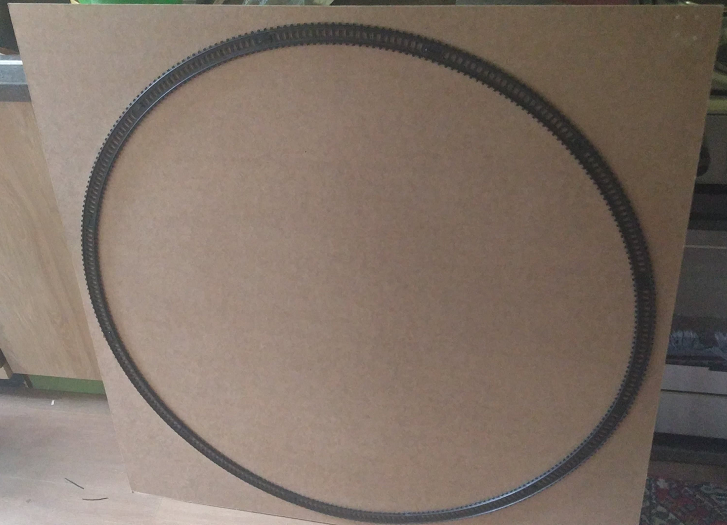
\includegraphics[width=\textwidth]{images/railnetworkplatformfront.png}
        \caption[Hálózat platform felül]{Hálózat platform felülnézete}
		\label{fig:railnetworkplatformfront}
    \end{minipage}\hfill
    \begin{minipage}{0.45\textwidth}
        \centering
        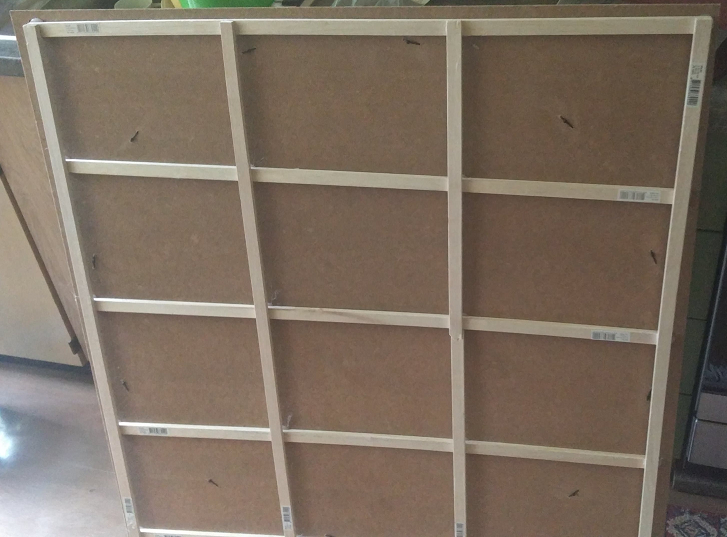
\includegraphics[width=\textwidth]{images/railnetworkplatfromback.png}
        \caption[Hálózat platform alul]{Hálózat platform alulnézete}
		\label{fig:railnetworkplatfromback}
    \end{minipage}
\end{figure}

\subsubsection{Jelző és észlelő platform}\subsubsectionro{Platforma pentru semnalizare și detectare}
A \ref{sec:mechspec}. fejezet szerinti specifikáció szerint, a 8 blokk méretű hálózatunknak, 8 darab jelző és észlelő platform szükséges.
A platformokat fekete $3mm$ vastagságú plexid lemezből készítettem, mivel tetszetős a színe és könnyen megmunkálható az anyag.
A jelző platformnak a három szín aspektus mellet, két rögzítési pontot is biztosítottam.
A rögzítést $4mm$-es hexagonális csavarokkal (apa, anya és dísz) oldottam meg.
A szín aspektusokat jelző LED-eknek tehát $3x7mm$-es, a rögzítésnek pedig $2x4mm$-es lyukakat készítettem a $40\times40mm$ méretűre tervezett lapra (\ref{fig:signalplatform}. ábra).
Az észlelőnek pedig $2x7mm$-es, az állapot LED-nek és szenzornak, és egy $4mm$-es, a rögzítésnek, lyukat fúrtam. Mérete pedig $20\times40mm$ (\ref{fig:vacancyplatform}. ábra).
Az alkatrész tartó lyukakban $7mm$ átmerőjű LED foglalatokat helyeztem.

\begin{figure}[htp]
    \centering
    \begin{minipage}{0.45\textwidth}
        \centering
        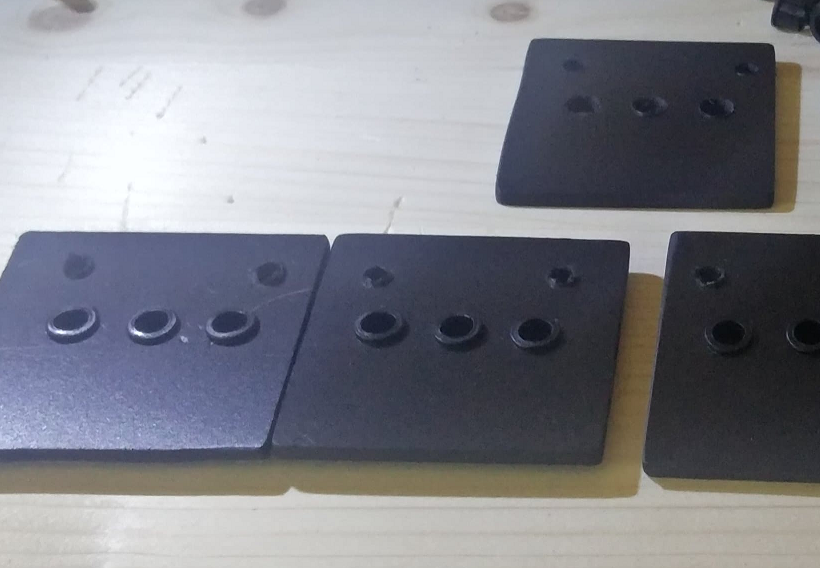
\includegraphics[width=\textwidth]{images/signalplatform.png}
        \caption[Jelző platform]{Elkészített jelző platform}
		\label{fig:signalplatform}
    \end{minipage}\hfill
    \begin{minipage}{0.45\textwidth}
        \centering
        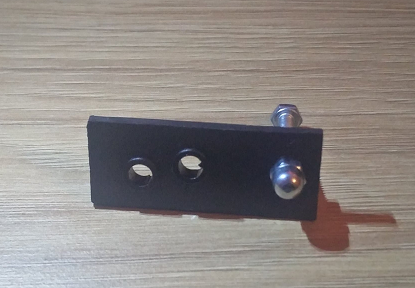
\includegraphics[width=\textwidth]{images/vacancyplatform.png}
        \caption[Észlelő platform]{Elkészített észlelő platform}
		\label{fig:vacancyplatform}
    \end{minipage}
\end{figure}

\subsection{Hardver kivitelezés}\subsectionro{Implementarea hardware-ului}
A rendszer hardver lelke az \textbf{Arduino Nano} fejlesztőlap. Ezt a fejlesztő lapot több okból kifolyólag választottam.
Első sorban egyszerűen és gyorsan felprogramozható, amint a \ref{sec:arduinonano}. fejezetben megbizonyosodhatunk róla.
Továbbá nagyon jó teljesítmény/költség aránnyal rendelkezik, a dolgozat írásának időpontjában 10-15 RON körül lehet beszerezni.
Végső sorban pedig kis fizikai méretezésnek köszönhetően, több rendszerben is egyszerűen integrálható. Éppen ezért mindegyik modul TM, SM, VM és ACC tartalmaz egy ilyen lapot a modul sajátos hardver vezérlése végett.
Valamint az információ továbbítás miatt, mindegyiket kibővítettem egy RFC kommunikációra képes RFT képes áramkörrel.
Ez a mi esetünkben a \ref{sec:rftcomm} fejezetben bemutatott \textbf{NRFL24} rádió frekvencia kommunikációs modul.
\subsubsection{Modulok közötti kommunikáció}\subsubsectionro{Comunicare între moduluri}\label{sec:RFTandRFC}
A \ref{sec:rftcomm} fejezetben leírt adatok alapján hardver szinten csak a \ref{tab:nrf24l01ports}. táblázathoz csatolt áramkört szükséges megvalósítani.
Az NRF24L01 által képviselt RFT-t SPT kommunikáció seftiségével vezérli a DB-MC.
Ezt a \ref{tab:nrf24l01ports} táblázatbeli port párosítás szerint végezzük el.

\begin{table}[htp]
	\begin{minipage}{0.5\linewidth}
		\centering
		\begin{tabular}{|c|c|}\hline
			DB-MC port & Megfelelő RFT port \\ \hline
			GND & GND \\ \hline
			3V3 OUT & $V_{cc}$ \\ \hline
			D9 & CE \\ \hline
			D10 & D10 \\ \hline
			D13/SCK& SCK \\ \hline
			D12/MISO & MOSI \\ \hline
			D11/MOSI & MISO \\ \hline
		\end{tabular}
	\end{minipage}\hfill
	\begin{minipage}{0.45\linewidth}
		\centering
		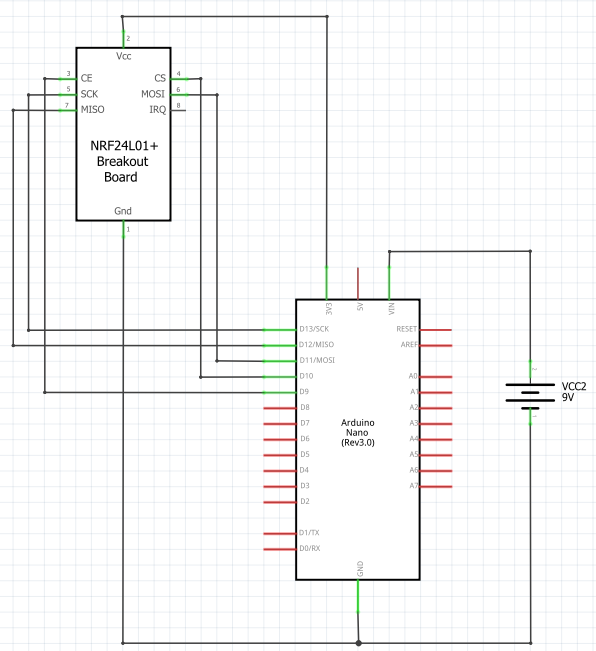
\includegraphics[width=0.7\linewidth]{images/RFTDBMCcircuit.png}
	\end{minipage}
	\caption[NRF24L01 bekötése]{NRF24L01 portjainak bekötése DB-MC-ben}
	\label{tab:nrf24l01ports}
\end{table}
Ezen túl hardver szinten nincs több feladatunk az RFT-vel kapcsolatosan, a rádiófrekvenciás hálózat és kommunikáció szoftver szintű vezérléssel valósul meg.

\subsubsection{Mozdony modúl}\subsubsectionro{Modulul de locomotivă}
A modell mozdony egy egyszerű, gyárilag, készen előállított, egyen árammal működő mozgó jármű. Tartalmaz egy egyenáramú motort, melyet egy 3 voltos elem telep hajt meg.
Valamint egy kapcsoló található rajta amit bekapcsolva, a mozdony azonnal mozgásba kerül.
Ez jelenti a kiindulási pontot. Célunk része ezt az egyszerű járművet digitalizálni, több funkcionalitás végrehajtására is képessé tenni, felhasználva a \textit{\nameref{theory_section}} fejezetben tanultakat.
A dolgozat keretein belül \ref{tab:hardspec}. táblázatban 1,2 és 3-as sorában leírt specifikációkkal bővítve a mozdonyt véglegesítjük a TM hardvert:

\begin{enumerate}
	\item \textbf{TM távirányítása}
	A \textit{\nameref{sec:RFTandRFC}} fejezetben leírtak alapján.
	\item \textbf{DC motor és vezérlése}
	A mozdonyban található gyári DC motornak csak a táplálási feszültségét ismerve első sorban meghatároztam ennek a maximális átjárási áramát.
	Ezt lemérve $I_{DCM_{max}} \approx 160 mA$ értéket kaptam. 
	Mivel a DB-MC technikai adatai szerint a digitális vezérlő portjai maximum  $40 mA$ képesek leadni, szükséges egy  külön szabályzó áramkör kialakítása.
	A motor sebesség szabályozást PWM modulációval oldottam meg. Figyelnünk kell arra is hogy a táplálás megszüntetése után a motor még mozgásban maradhat, és ezáltal generátor módban kerül. 
	Az ilyenkor fellépő visszáramtól védnünk kell a a DB-MC-t.
	Ezekre a kritériumokra alapozva az \ref{fig:TMDCMC}. ábrán látható áramkört terveztem. 
	A motort egy külön 3V-os PSU táplálja, az ebben az áramkörben potenciálisan átfolyó nagy áramot így elszigeteljük a DB-MC áramköreitől.
	Az áthaladó áramot a DB-MC D6-os, PWM képes, portjáról vezéreljük egy tranzisztorral kapcsoló üzemmódban.
	Konkréten egy 2n2222 modellű NPN tranzisztor bázis áramának segítségével nyitjuk vagy zárjuk a motort hajtó áramkört.
	A tranzisztor adatlapja szerint $I_{C} = 600 mA$ folytonos kollektor áramot képes szolgáltatni \cite{os2n19}, ami teljes mértékben megfelel a mi alkalmazásunkra.
	A tranzisztor bázisára szükséges egy $R_{T_{B}} = 1k\Omega$-os áram korlátozó ellenállást is helyezni, védve a tranzisztor hibásodását túl nagy bázis áram esetén.
	A visszáram kivédését egy egyszerű 1N4004-es diódával oldjuk meg, a katód kivezetését a motor pozitív kivezetésére kötve garantálni tudjuk hogy generátor mód esetén nem folyik vissza semmilyen áram.
	A konkrét PWM modulációt a TM DB-MC-n futó program valósítja meg, hardver szemszögből elégséges a az áramkör vezérlést PWM képes portra kötni.
    \begin{figure}[htp]
        \centering
        \begin{minipage}{0.5\textwidth}
            \centering
		    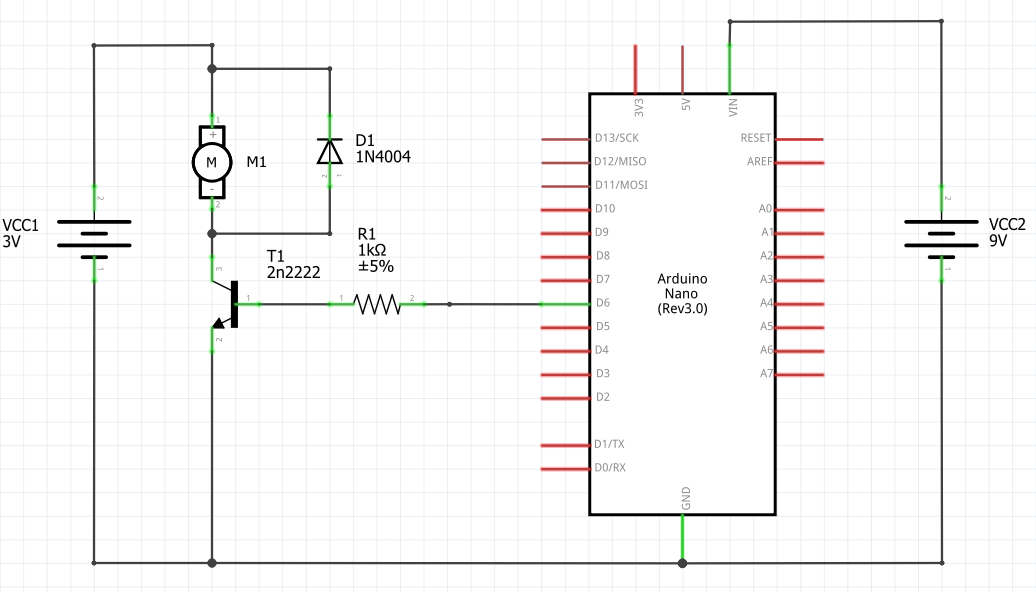
\includegraphics[width=\linewidth]{images/TMDCMC.png}
		    \caption[Motor vezérlés]{A DC motor vezérlő áramkör}
		    \label{fig:TMDCMC}
        \end{minipage}\hfill
        \begin{minipage}{0.45\textwidth}
            \centering
		    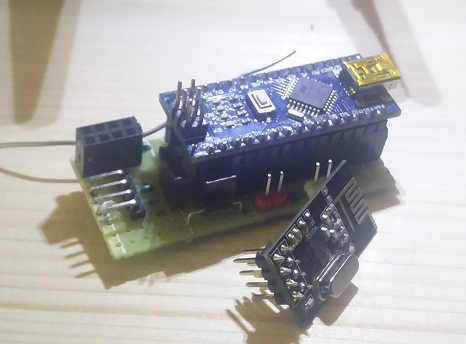
\includegraphics[width=0.9\linewidth]{images/TMboard.png}
	    	\caption[TM implementáció]{Végleges TM nyák kivitelezés}
	    	\label{fig:TMboard}
        \end{minipage}
    \end{figure}
	A TIP funkciót egyszerűen egy fehér színű led aktiválásával valósítottam meg.
	A LED a mozdony közepére van rögzítve. Bal oldali irányban bocsájtva ki fényét.
	A LED a DB-MC D8-as portjára, digitális kimenet módban, vezérelt. 
	Itt is figyelni kell az áramokra, mivel a DB-MC digitális kimenet módban 5V-ot szolgáltat.
	Egyenesben kötve a LED-nek 2V-ra van csak szüksége, megkárosítaná a nagyobb feszültség.
	Ezért itt is $R_{LED} = 220\Omega$-os áram korlátozó ellenállásokat kötünk a LED és a kimeneti port közé.
\end{enumerate}

Az így felépített TM végleges panelre ültetett kivitelezése látható a \ref{fig:TMboard}. ábrán, a modellre szerelt vezérlés a \ref{fig:TMmodell}. ábrán,  valamint a teljes tervezett áramkör a \ref{fig:circuit_train_module}. ábrán:


\begin{figure}[!htp]
	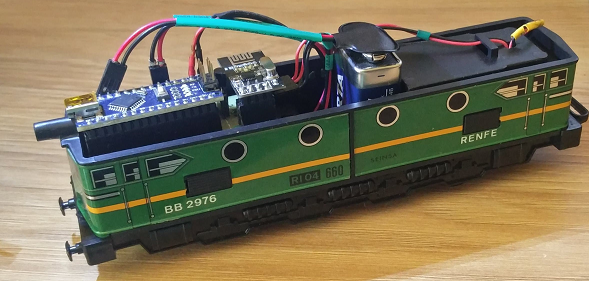
\includegraphics[width=\linewidth]{images/TMmodell.png}
    \caption[TM modellel]{TM vezérlés modellbe szerelve}
	\label{fig:TMmodell}
\end{figure}

\begin{figure}[!htp]
	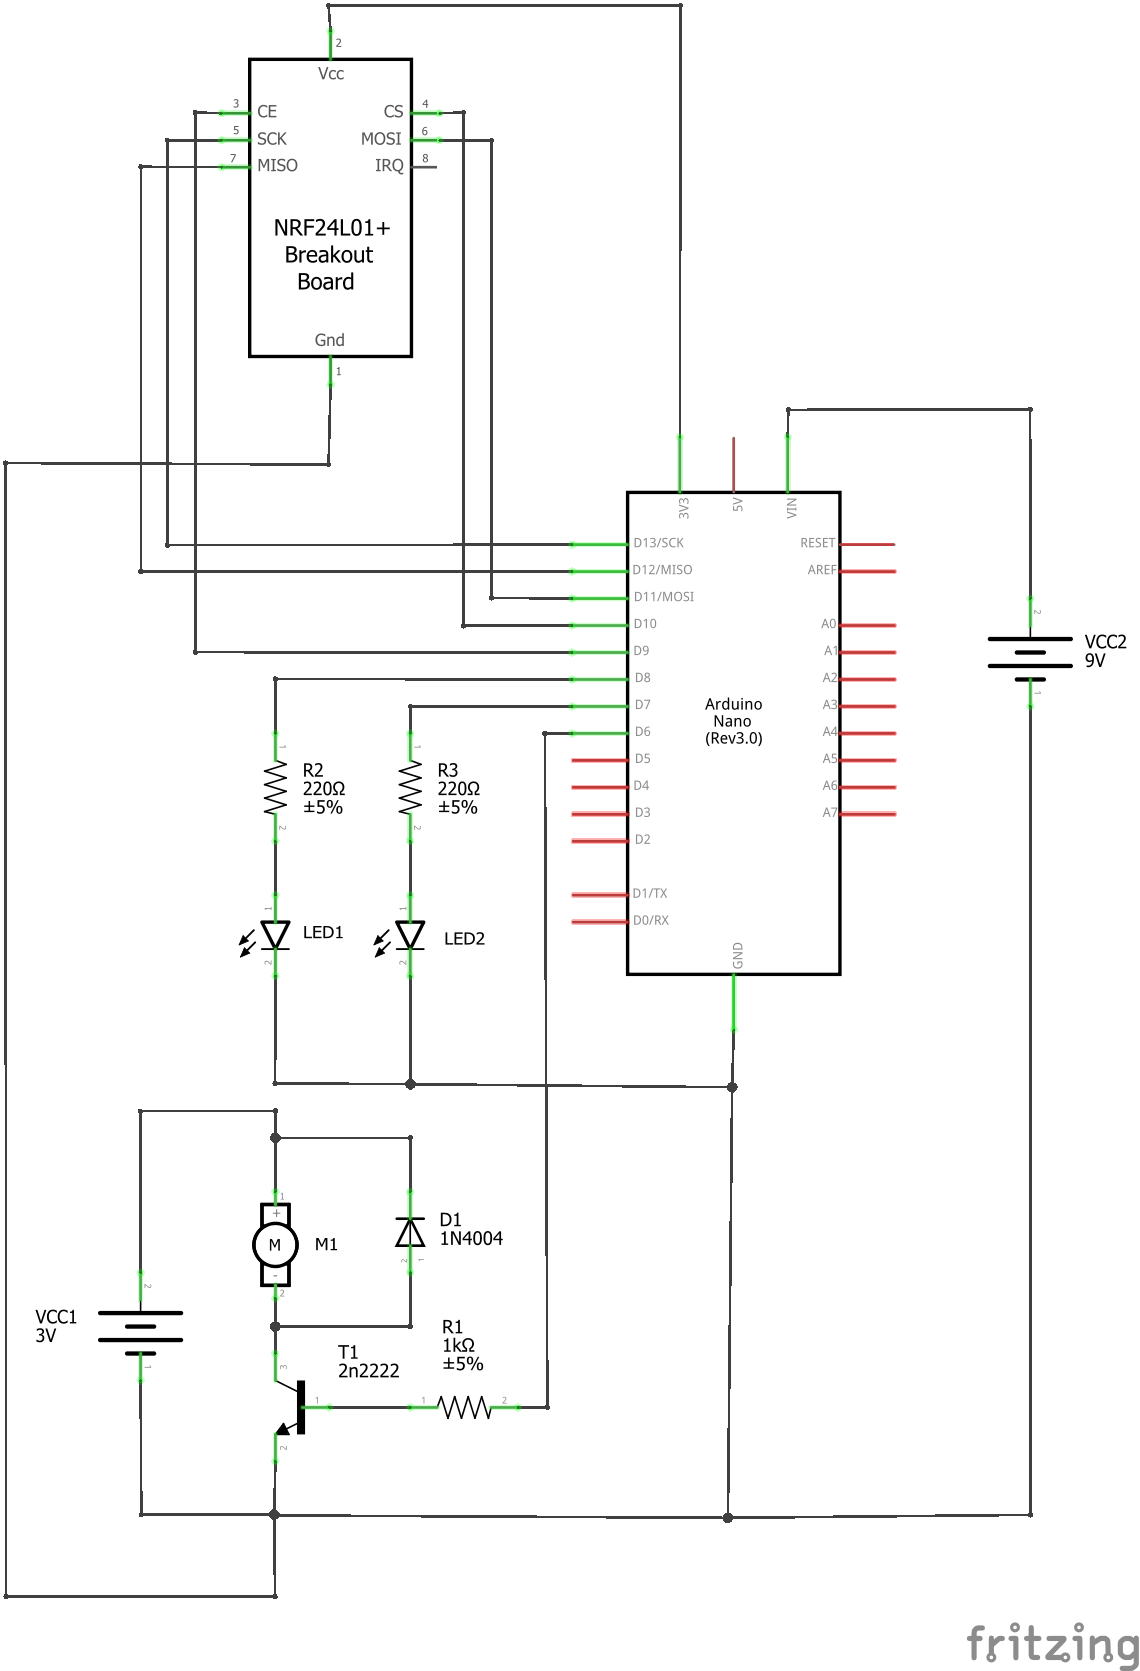
\includegraphics[width=0.9\linewidth]{images/circuit_train_module.png}
    \caption[Modell mozdony modul áramköri rajza]{Modell mozdony modul áramköri rajza}
	\label{fig:circuit_train_module}
\end{figure}

\newpage



\subsubsection{Észlelő hálózat}\subsubsectionro{Rețeaua de detectare}
Az VM hardver része lényegében egy LDR szenzor bemenetére reagáló áramkör.
A \ref{tab:hardspec}. táblázat szerinti 4. specifikációt valósítjuk meg.
A 8 blokk definíciója szerint, mindegyik blokkban szükséges egy ilyen szenzor elhelyezése.
Az LDR áramkörök egy egyszerű LDR szenzor és  egy $R_{LDRx} = 220\Omega$-os ellenállás sorba kötésével valósítottam meg.
A két ellenállás közötti részt kötjük a DB-MC analóg bemenet portjaira(A0-A7). Itt a fény hatására a bementi analóg port érzékeli a feszültség változást.
Ezt a változást pedig a DB-MC belső ADC-je átalakítja egy 10 bites digitális értékre.
A változást a szenzor előtt elhaladó TM modell TIP implementációja idézi elő.
A 8 darab LDR áramkört mindegyikét a DB-MC 5V-os kimenete táplálja.

Megjegyezendő itt hogy az LDR-nek az ohmikus ellenállása maximális fényerőnél minimum $R_{LDR_l} = 2 k\Omega$, sötétben pedig $R_{LDR_d} = 150 k\Omega$.
Ismerve ezeket a paramétereket Ohm és Kirchhoff-csomópont törvényekre alapozva, kiszámíthatjuk az össz. áramfogyasztás min-max intervallumát.
\begin{equation}
 I = \frac{U}{R}; I_{total} = I_{1} +I_{1} + I_{2} +... + I_{n}   
\end{equation}
Ohm törvénye alapján egy LRD áramkör ágon, maximum $I_{LDR_1} = 2 mA$, minimum  $I_{LDR_1} = 3 \mu A$ áram folyik át.
Kirchhoff törvénye alapján pedig összesen $I_{total_{max}} = 8 \times 2 mA = 16 mA$, valamint $I_{total_{min}} = 8 \times 3 \mu A= 24\mu A$.
A DB-MC 5V-os portja képes $200 mA$-t leadni. Tehát biztosan az LDR áramköreink nem fogják káros áramoknak kitenni a DB-MC-t.

Validációs szemszög miatt a DB-MC-re további 8 darab kék színű állapot LED-et is kötöttem a DB-MC D1-D8 portjaira, digitális kimeneti szereppel.
Ezt azért tettem, hogy majd a szoftver feldolgozott szenzor adatait, vizuálisan is megerősítse a felhasználó számára.
Az az ha a szenzor egy érvényes bemenetet érzékel, a VM DB-MC-je bekapcsolja a neki megfelelő LED-et. 
Tehát mindegyik LDR áramkörnek megfelel egy állapot LED áramkör is. 
A bekapcsolt LED aktív bemenetet jelent a szenzor oldalon, inaktív LED pedig értelemszerűen ennek ellenkezőjét.

A begyűjtött adatok továbbításáért ez esetben is a \textit{\nameref{sec:RFTandRFC}} fejezetben leírt RFT felelős.


A \ref{fig:VMLDRelement}. ábrán egy elkészített VM komponens látható, ennek láthatóan 4 bemeneti portja van.
Egy az LDR áramkör táplálása, egy az analóg kimenet érzékelése, egy az állapot LED vezérlése, és végül egy a GND miatt.

A 8 darab LDR komponens végül a \ref{fig:VMDMBCRFT}. ábrán látható VM modul nyákhoz kerül bekötésre.

\begin{figure}[htp]
	\centering
	\begin{minipage}{0.5\textwidth}
		\centering
		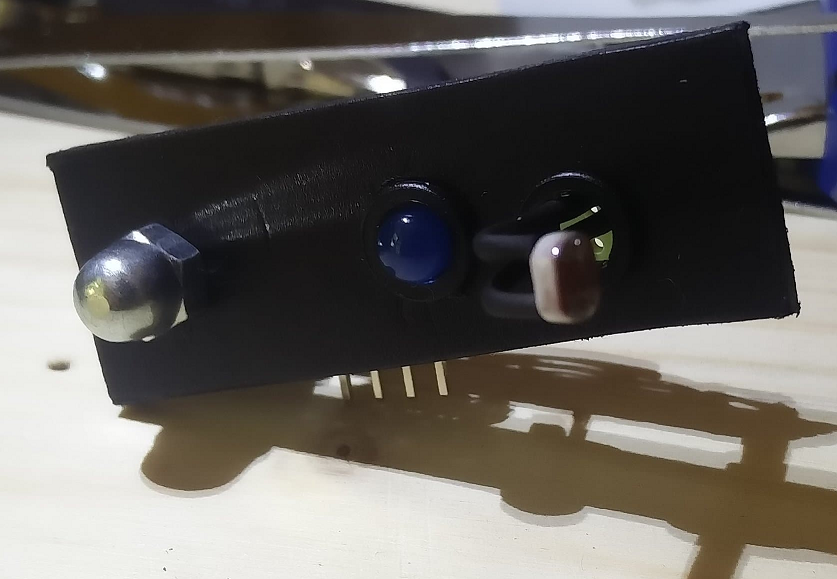
\includegraphics[width=0.8\linewidth]{images/VMLDRelement.png}
		\caption[Egy LDR komponens]{Kivitelezett LDR komponens egyike}
		\label{fig:VMLDRelement}
	\end{minipage}\hfill
	\begin{minipage}{0.45\textwidth}
		\centering
		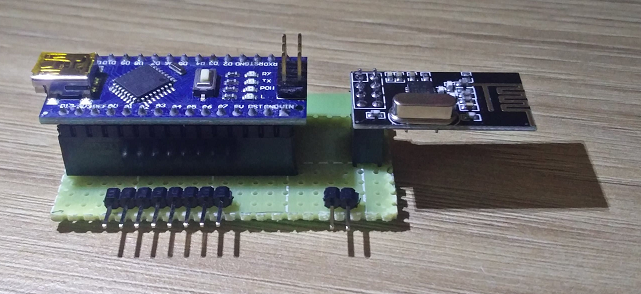
\includegraphics[width=\linewidth]{images/VMDMBCRFT.png}
		\caption[VM implementáció]{Végleges VM nyák kivitelezés}
		\label{fig:VMDMBCRFT}
	\end{minipage}
\end{figure}


Végül pedig a modell VM hálózat kivitelezett áramköre látható a \ref{fig:circuit_vacancy_module}. ábrán:

\begin{figure}[!htp]
    \centering
	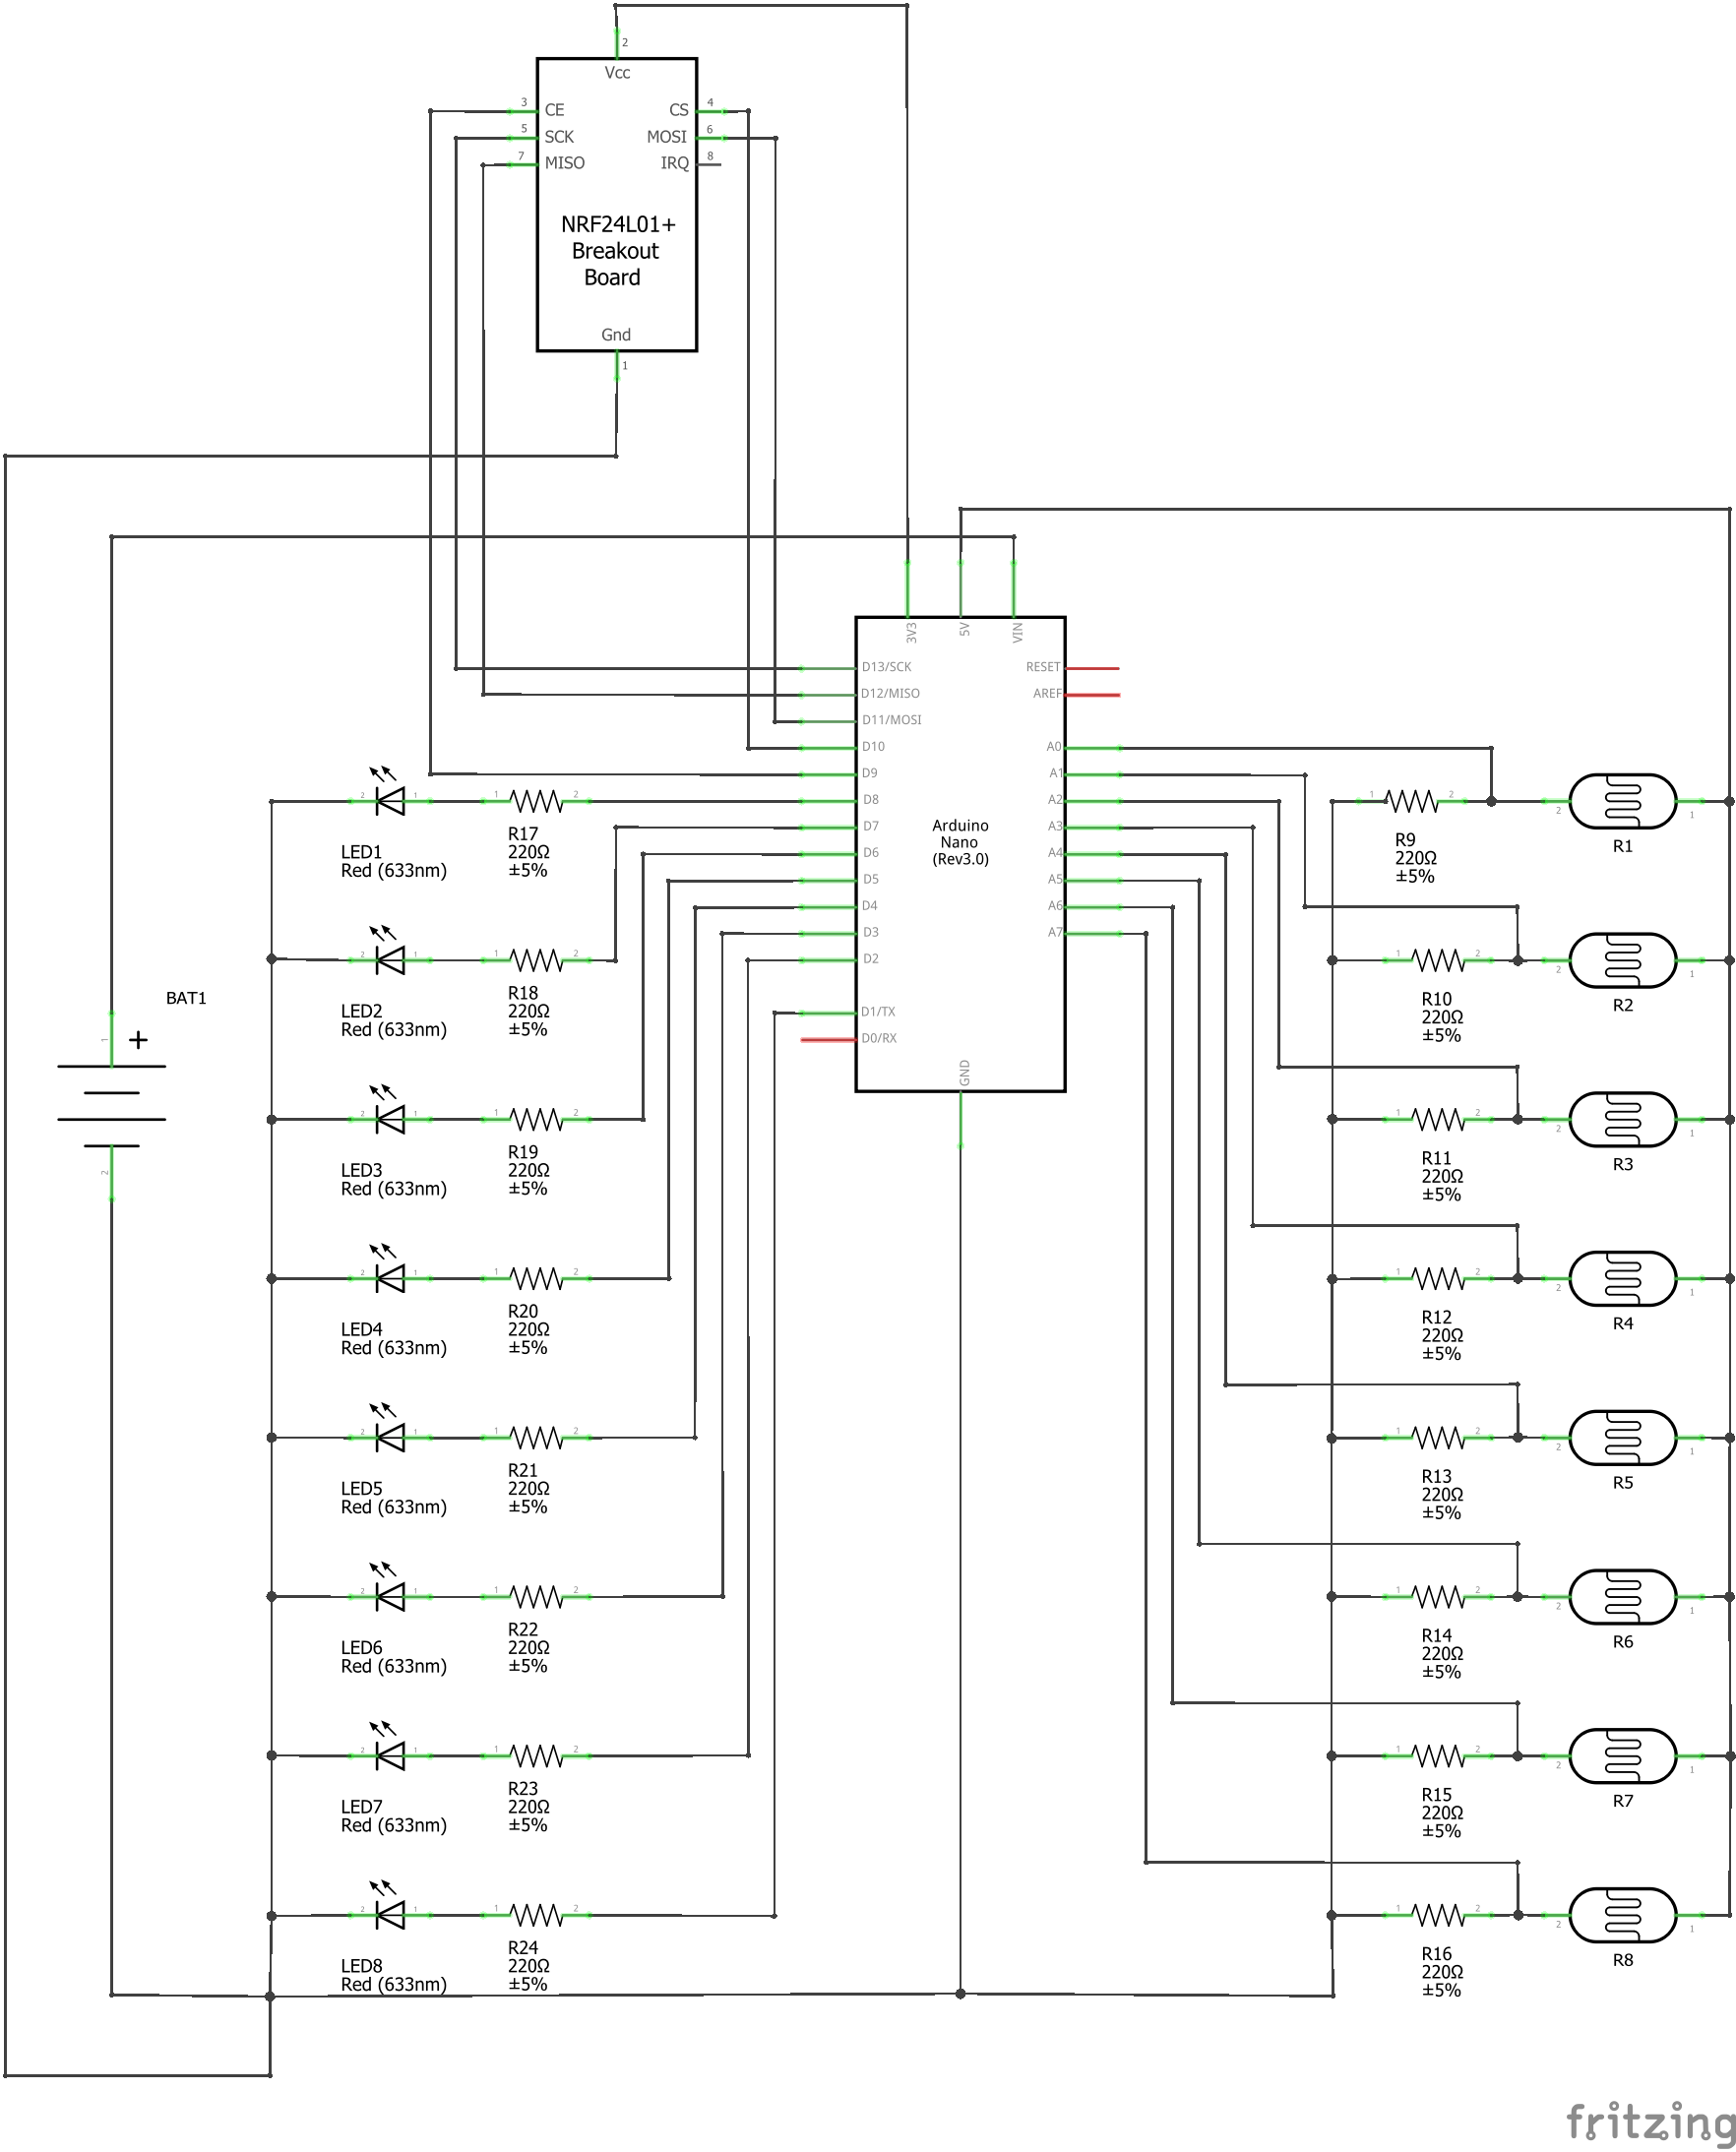
\includegraphics[width=0.8\linewidth]{images/circuit_vacancy_module.png}
    \caption[Modell észlelő hálózat modul áramköri rajza]{Modell észlelő hálózat modul áramköri rajza}
	\label{fig:circuit_vacancy_module}
\end{figure}

\newpage
\subsubsection{Jelző hálózat}\subsubsectionro{Rețeaua de semnalizare}
A SM hálózat szerepe a mozdony vezető számára megfelelő jelző aspektust szolgáltatni, ahhoz hogy az előbbi biztonságos sebességgel tudjon közlekedni a vágányhálózaton.
Itt is a korábban említett 8 blokk, 8 darab SM komponenst határoz meg.
Ezek lényegében 3 led, egy piros, egy sárga és egy zöld vezérléséből valósul meg, a nekik megfelelő $R_{LED} = 220\Omega$-os áramkorlátozó ellenállással.
Ez megfelel a \ref{tab:aspectandcolor}. táblázatban ábrázolt aspektus típusoknak.
Értelemszerűen $8\times 3 = 24$ darab LEDet fog kelleni vezérelni.
Itt egy kis gond akad, mivel a DB-MC-nek, a \ref{tab:arduino_pint_out}. táblázat szerint, csak 14 digitális kimeneti portja van.
Ezért a 24 LED vezérléshez 3 darab 8 bites shift regisztert használtam.
A regisztereket nem kötöttem össze "vízesés" módban, mivel így elég digitális kimenet felszabadult a DB-MC-n ahhoz hogy mindegyiket külön tudja vezérelni.
A regiszterek a \textit{\nameref{sec:shiftregister}}. fejezetben leírtak alapján működnek.
Lényegében mindegyik regiszter 8 LED-et képes vezérelni, tehát a 3 regiszter vezérlését a D0-D8 digitális kimenetekkel oldjuk meg.
Hármas csoportokban rendre a regiszterek $DS$, $ST_CP$, $SH_CP$ portjaira kötöttem a DB-MC kimeneteket.
A  $V_{cc}$ portokat a DB-MC 5V-os kimenetére, az OE portot a földre (mivel a regiszter megtagadja ezt a bemenetét, és földre kötve mindig aktív lesz a regiszter kimenete) kötöttem.
Továbbá a maradék MR portot is a  DB-MC 5V-os kimenetére kötjük(digitális \textit{HIGH}-t folyamatosan tartva, nem törli ki a regiszter tartalmát), a regiszter GND-ját pedig a DB-MC GND-ra.
Mivel egy regiszter egy adott pontban maximum 3 LED-et kell meghajtson, itt sem fog gondot jelenteni az áram ellátás.
Szem előtt kell tartani hogy annak ellenére hogy minden VM komponens három LED-et tartalmaz egy adott időben mindig csak szigorúan egyik lesz érvényes.
Tehát teljes hálózatra számolva 8 LED lehet aktív egy adott időben.

Az SM komponensek vezérléséért az ACC felelős, az adatok pedig a \textit{\nameref{sec:RFTandRFC}} fejezetben leírt RFT hálózaton keresztül érkeznek meg.
Egy komponensnek 4 csatlakozási portja van, 1 GND valamint 1-1 port a három aspektus vezérlésére, \ref{fig:SMelement}. ábra.
Végül pedig össze szereltem a teljes SM nyákot, a 24 vezérlő porttal, 3 regiszterrel, DB-MC és RFT alkatrészeivel, \ref{fig:SMDBMCRFT}. ábra.


\begin{figure}[htp]
	\centering
	\begin{minipage}{0.5\textwidth}
		\centering
		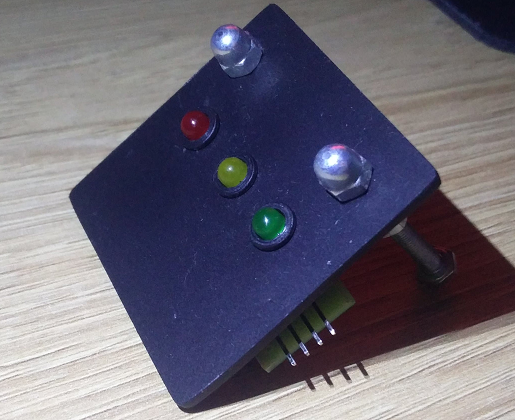
\includegraphics[width=0.75\linewidth]{images/SMelement.png}
		\caption[Egy SM komponens]{Kivitelezett SM komponens egyike}
		\label{fig:SMelement}
	\end{minipage}\hfill
	\begin{minipage}{0.45\textwidth}
		\centering
		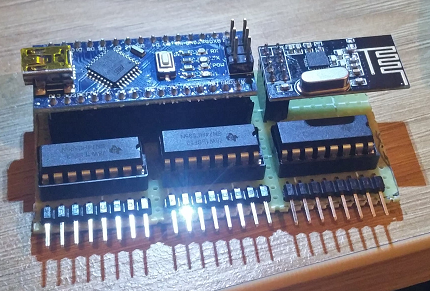
\includegraphics[width=0.9\linewidth]{images/SMDBMCRFT.png}
		\caption[SM implementáció]{Végleges SM nyák kivitelezés}
		\label{fig:SMDBMCRFT}
	\end{minipage}
\end{figure}

A SM hálózat tervezett teljes áramköre látható a \ref{fig:circuit_signal_module}. ábrán:

\begin{figure}[!htp]
	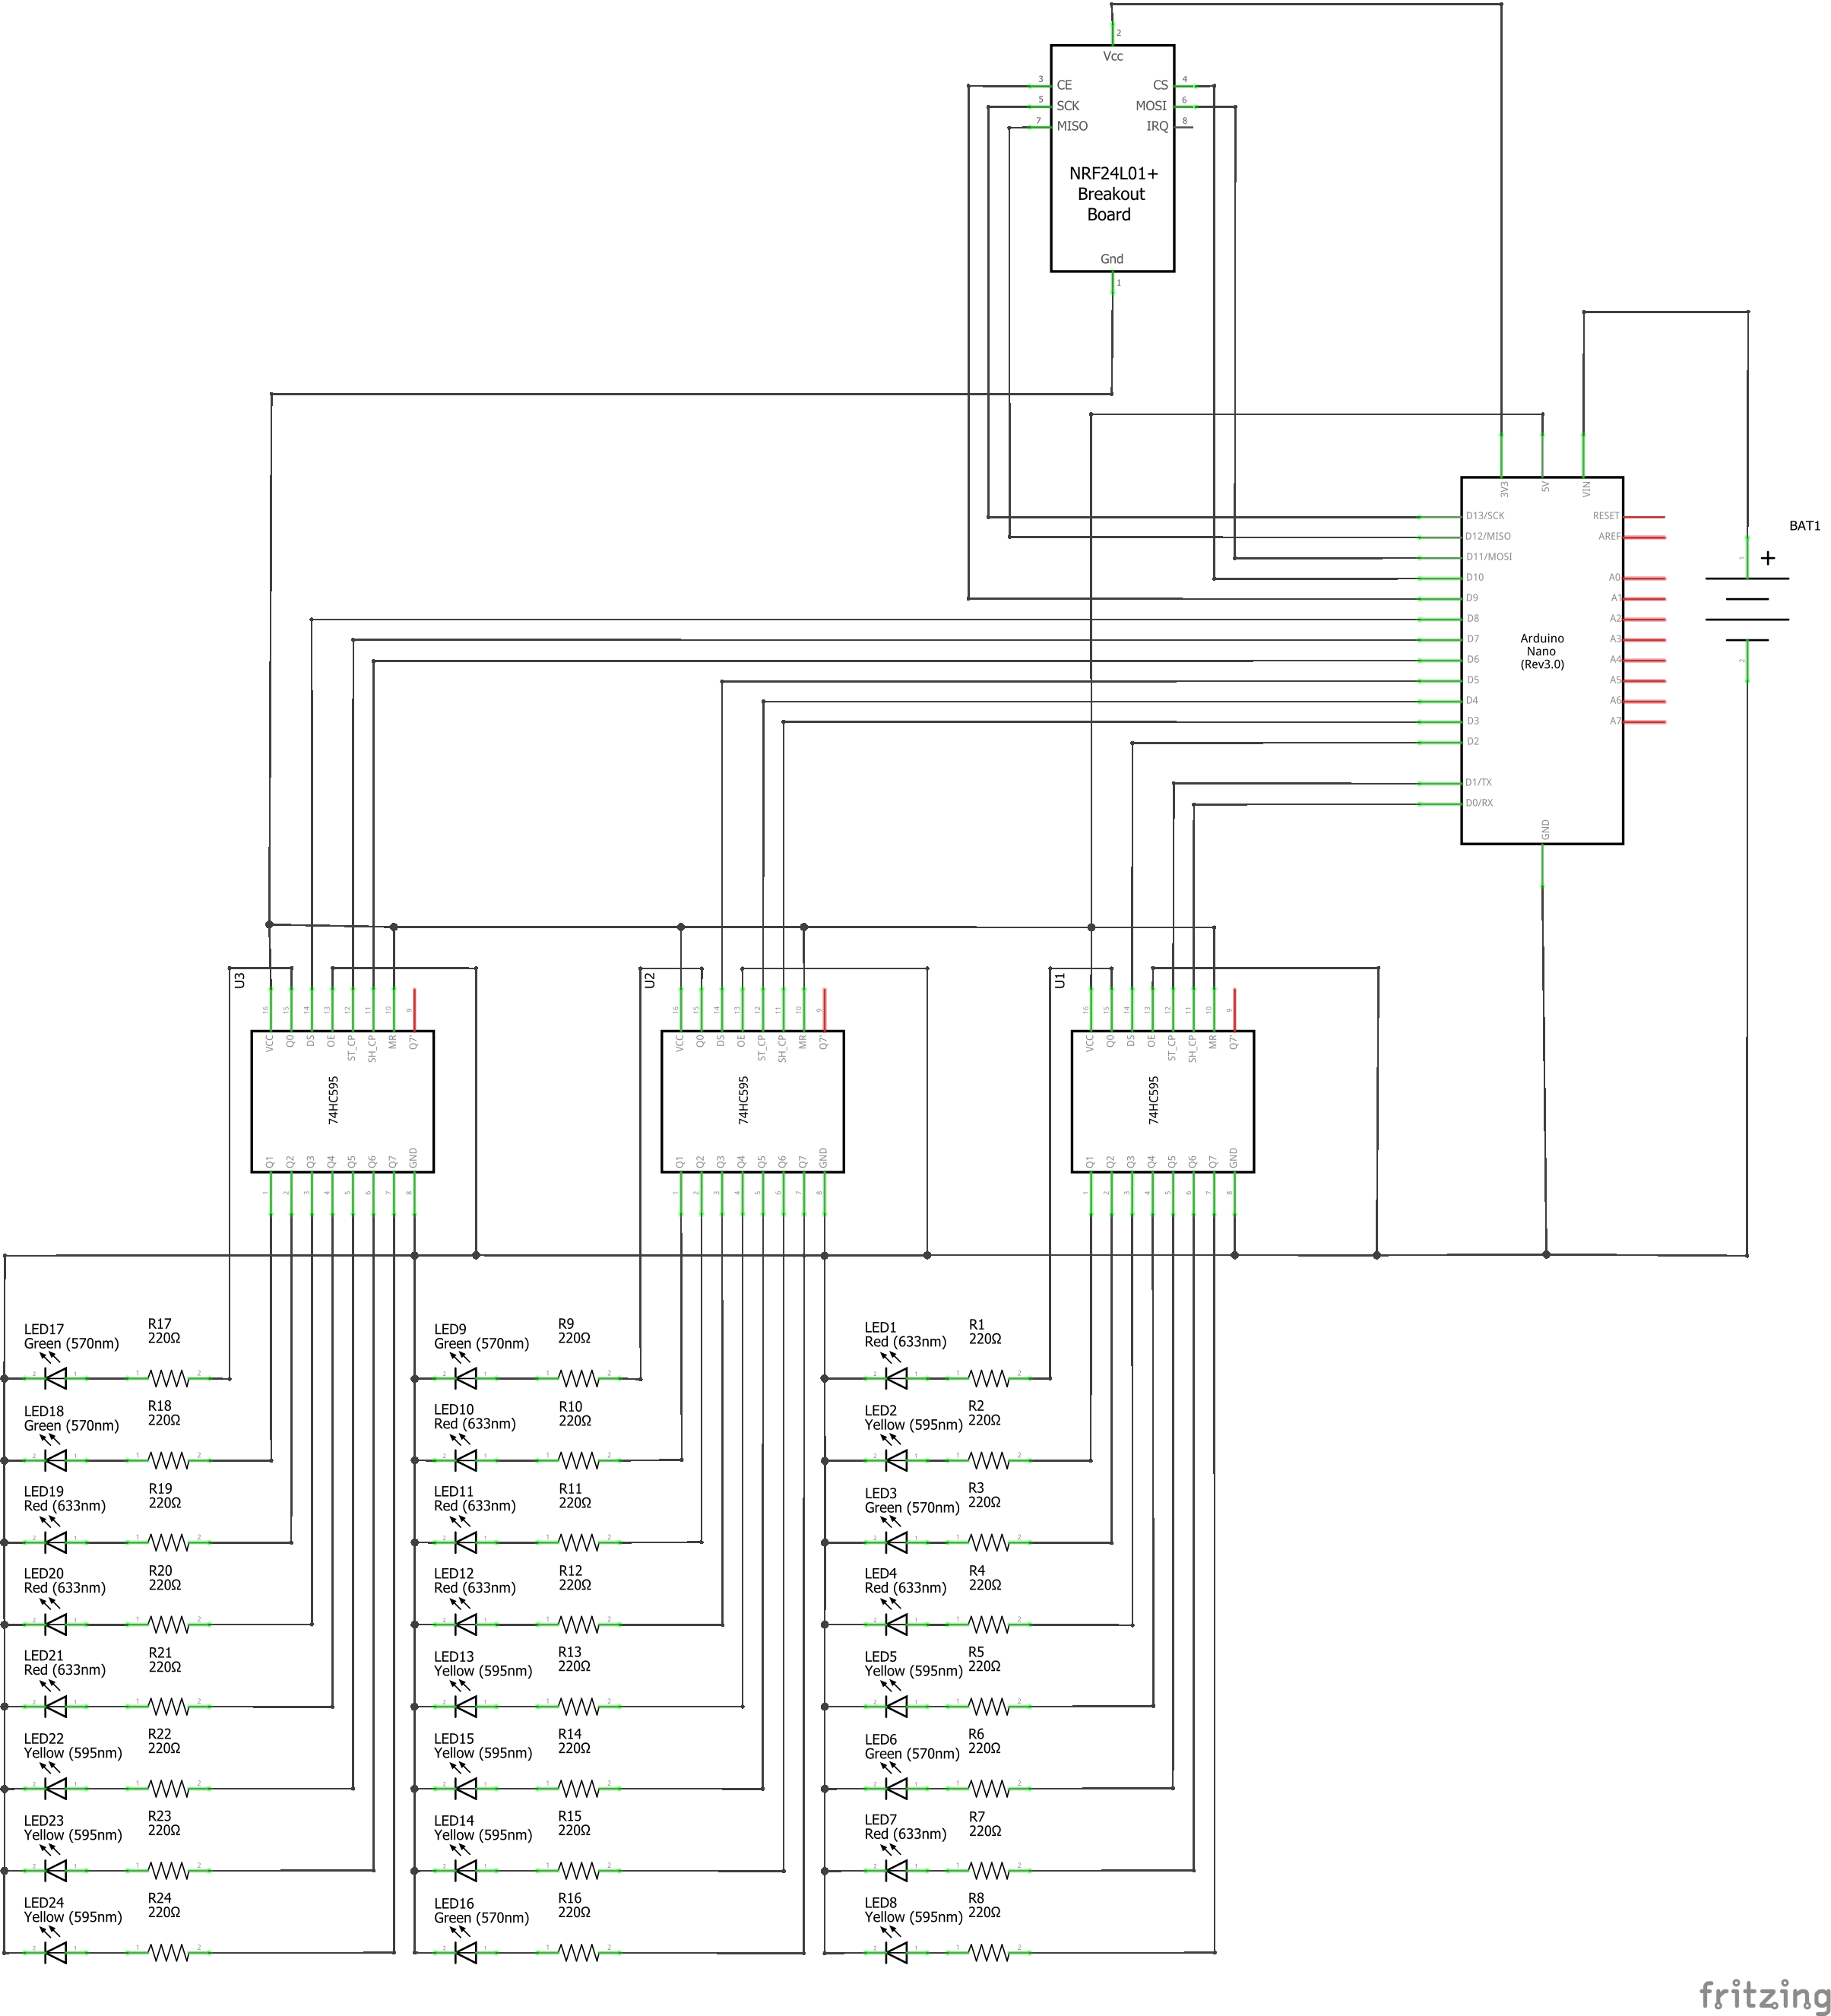
\includegraphics[width=\linewidth]{images/circuit_signal_module.png}
    \caption[Modell jelző hálózat modul áramköri rajza]{Modell jelző hálózat modul áramköri rajza}
	\label{fig:circuit_signal_module}
\end{figure}



\subsubsection{Központi vezérlő módul}\subsubsectionro{Modulul central de control}

\begin{wrapfigure}{l}{0.50\textwidth}
	\vspace{-20pt}
    \centering
    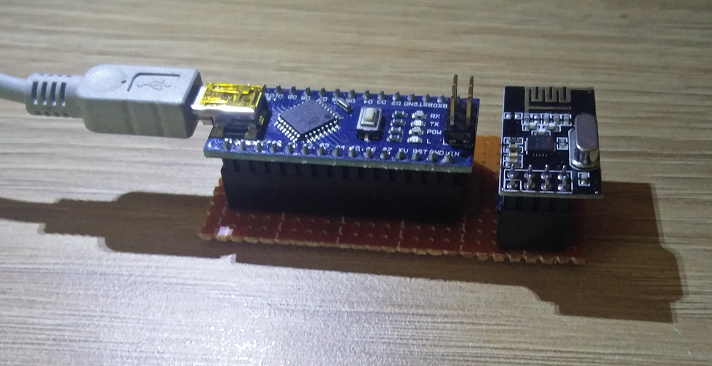
\includegraphics[scale=0.5]{images/ACCRFT.png}
    \caption[ACC implementáció]{ACC nyák kivitelezés}
    \label{fig:ACCRFT}
\end{wrapfigure}

Az ACC hardverileg a legegyszerűbb része a rendszerünknek (\ref{fig:ACCRFT}. ábra).
Hardverileg csak a DB-MC és \textit{\nameref{sec:RFTandRFC}} fejezetben leírt RFT áramkörből áll.
Az egyetlen eltérést a folyamatos kommunikációs kapcsolat, az USB-USB B portokon keresztül a TC-GUI és RN-GUI-val, jelenti.
Külső táplálásra ez esetben nincs szükség, mivel az USB kapcsolat szolgáltatja a szükséges táplálást.
Maga a soros kommunikáció a DB-MC D0 és D1 (RX valamint TX módban) valósul meg.
Megjegyezzük hogy a TM modul mobilitása miatt elem telepekkel tápláljuk.
Az SM és VM modulok pedig egy az RN platformra rögzíttet $230V\rightarrow 9V$ adapterrel történik, melynek a maximális áram leadó képessége $2A$.
Végül a központi vezérlő módul megvalósított áramköre látható a \ref{fig:circuit_central_module}. ábrán:

\begin{figure}[!htp]
    \centering
	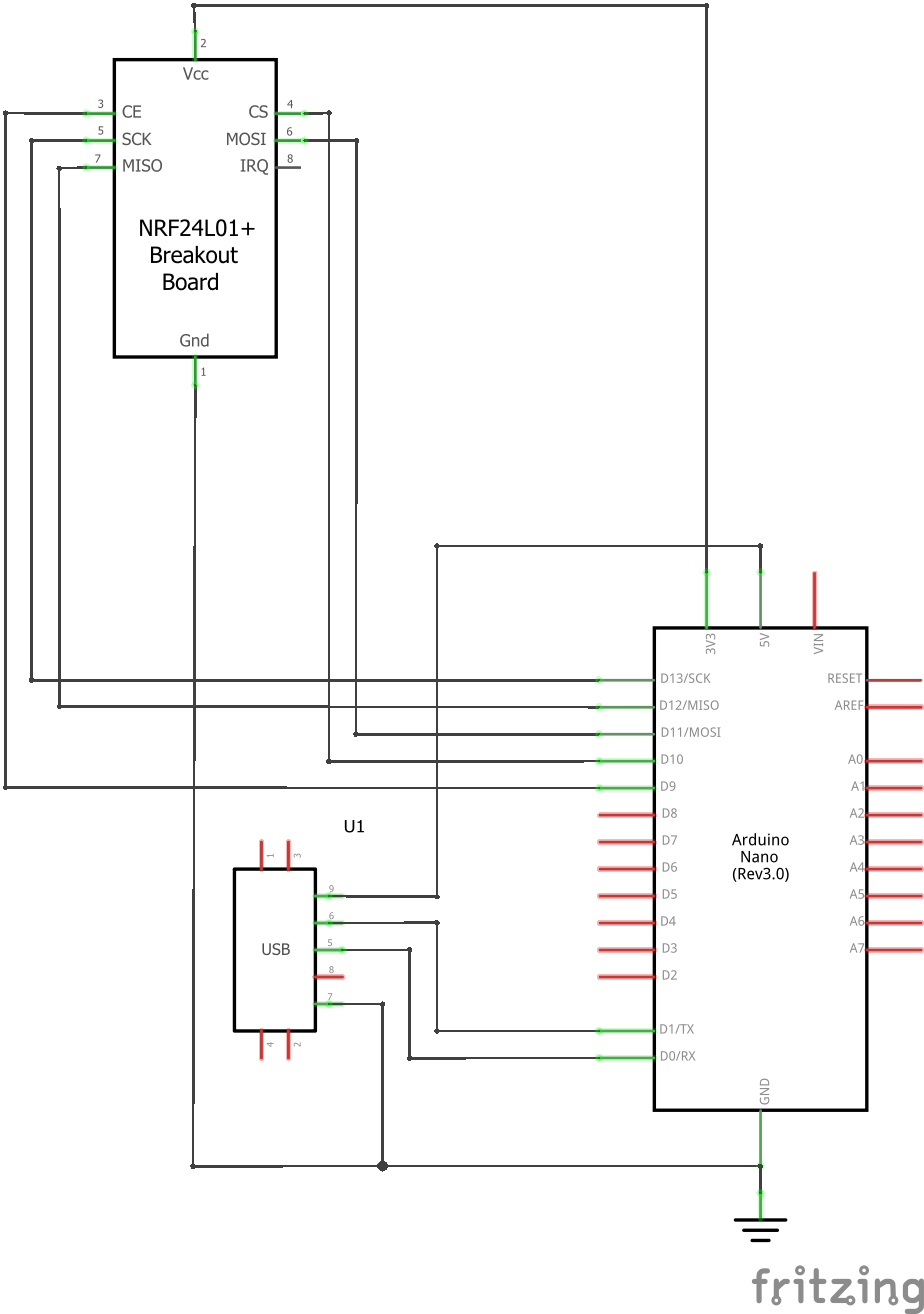
\includegraphics[scale=1]{images/circuit_central_module.png}
    \caption[Központi vezérlő módul áramköre]{Központi vezérlő módul áramköre}
	\label{fig:circuit_central_module}
\end{figure}


\newpage
\subsection{Szoftver kivitelezés}\subsectionro{Implementarea software-ului}
A szoftver megvalósítás a \ref{tab:softspec}. táblázatban összefoglalt specifikációkat követve történt.
Itt fontos megemlíteni hogy az RFC megvalósítás közös pont mindegyik komponensben, leszámítva a grafikus interfészt.
A rendszerben történő adatáramlást lebontva a komponensek alrészeire a \ref{fig:ra_data_flow_diagram}. ábra mutatja be:

\begin{figure}[htp]
    \centering
	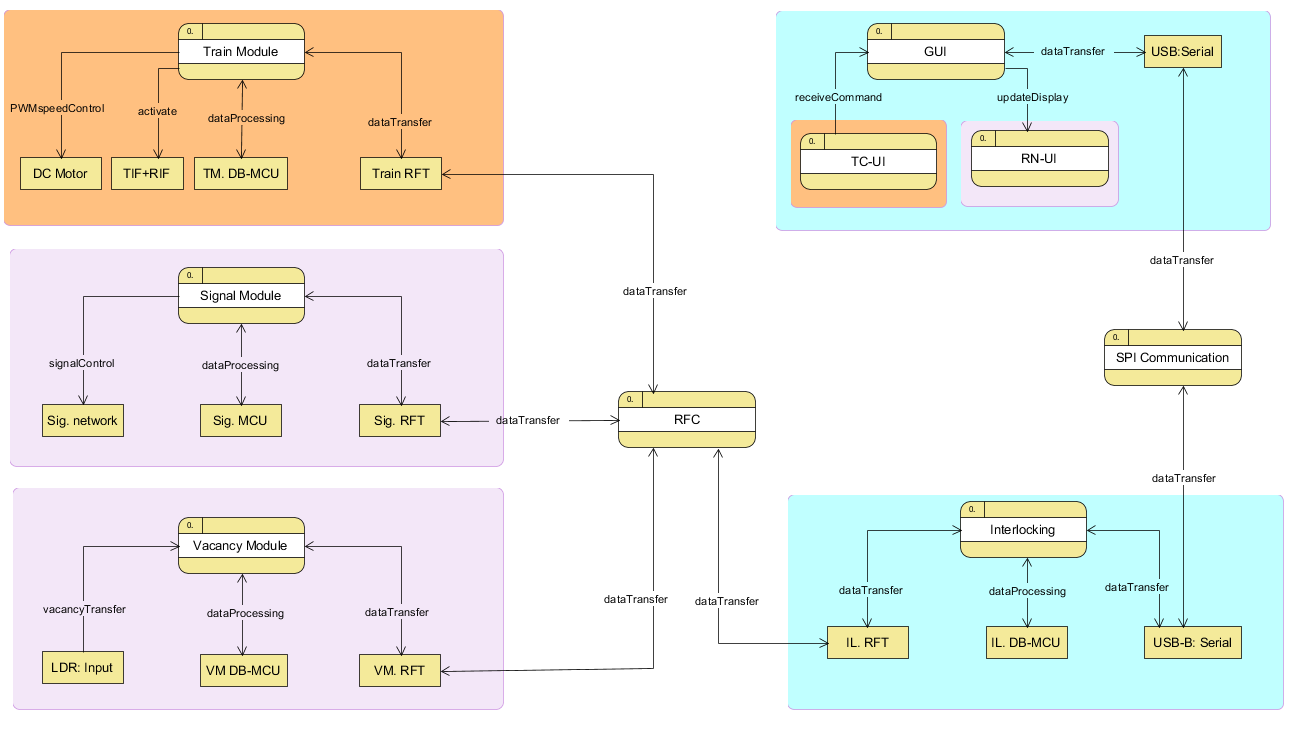
\includegraphics[width=\textwidth]{images/ra_data_flow_diagram.png}
    \caption[Rendszer folyamat architektúra]{Megvalósított rendszer folyamat architektúrája}
	\label{fig:ra_data_flow_diagram}
\end{figure}
Látható hogy a GUI részről a sebesség kiválasztása a TM számára jelenti a kiinduló pontot, amely soros USB porton keresztül az ACC-hez továbbítódik.
Az ACC a központi ügynökünk aki fogadja, értelmezi és továbbítja a beérkező információkat.
A kiválasztott sebsebég módot RFC-n keresztül továbbítja a TM-nek amely mozgásba hozza a mozdonyt.
A mozdony aktiválja a TIP funkciót, amely szenzor bemenetet szolgál a VM-nek.
A VM feldolgozza az adatot és továbbítja ugyancsak RFC-n keresztül az összes blokk állapotát az ACC fele.
Az ACC a fogadott csomagot jelző aspektus szekvenáló algoritmusával értelmezi, és kiszámolja a szükséges biztonsági aspektust mindegyik blokknak.
Az új aspektusokat tartalmazóz csomagot, RFC segítségével, továbbítja az SM-nek. Ugyanakkor az észlelt VM bemenetet és a számolt aspektusokat továbbítja a RN-GUI fele is, kijelzésre.
Az SM miután megkapta a csomagot, feldolgozza, átalakítja, sajátos algoritmussal, olyan formában hogy a három shift regiszter bemeneteire vezethető legyen.
Végül elérve az aspektusok megjelenését a jelző hálózatban.

A rendszer szekvencia diagramja a fentebb leírt folyamat egy ciklusát ábrázolja a \ref{fig:ra_sequence_diagram}. ábrán. 
Termesztésen ez a folyamat, megszakítás nélkül ismétlődik a rendszer lekapcsolásának pillanatáig.
Az összes komponens létfontosságú, a rendszer nem működő képes biztonságos körülmények között ha bármelyik is, például hardver vagy szoftver hiba miatt, kiesik.

\begin{figure}[htp]
    \centering
	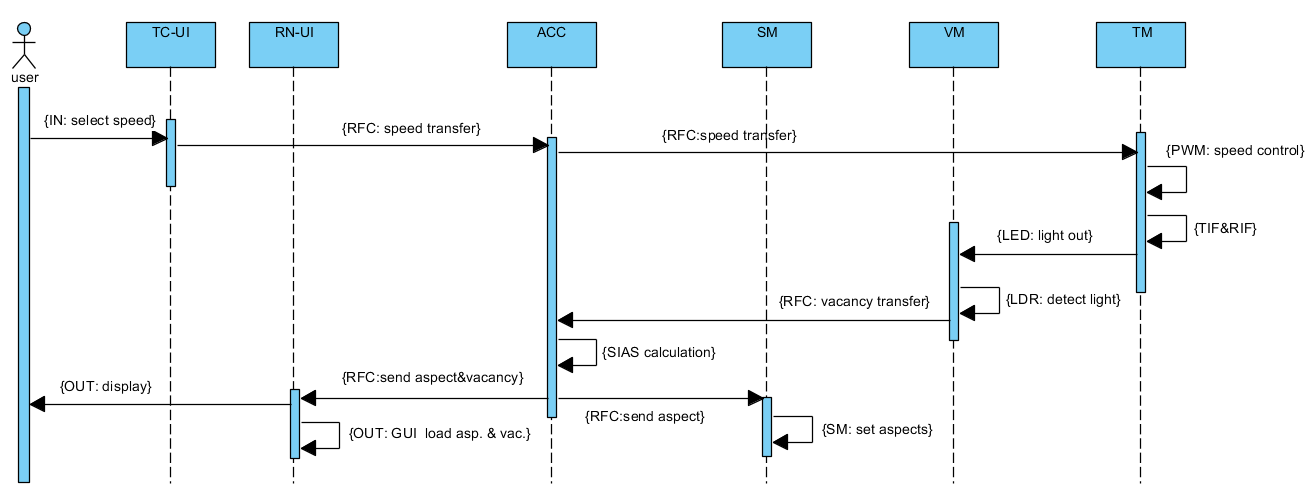
\includegraphics[width=\textwidth]{images/ra_sequence_diagram.png}
    \caption[Rendszer szekvencia diagram]{Megvalósított rendszer szekvencia diagramja}
	\label{fig:ra_sequence_diagram}
\end{figure}

\subsubsection{Modulok közötti komunikáció}\subsubsectionro{Comunicare între moduluri}
A szoftver specifikációban több pontban is említve van az RFT által megvalósított RFC kommunikáció.
A hardver megvalósítás szerint, 4 darab RFT áramkört használ a rendszer.
A \textit{\nameref{sec:nrlf24rfc}} fejezetben leírtak alapján ezek közös hálózati csatornán kommunikálnak egymással.
A \ref{tab:rftadress}. táblázatban összefoglaltam ezeknek a fontosabb paramétereit.
A modulok címe nyolcas számrendszerben van megadva, valamint a szoftverben ennek a tízes számrendszeri megfelelőjét is használjuk, a fejlesztet könyvtár csomag típus követelményei miatt.
Mint látható az ACC a brókerünk, mint a biztosító rendszer központi része, a többi modul csak küld vagy fogad adatot tőle.

\begin{table}[htp]
    \centering
    \begin{tabular}{|c|c|c|c|}\hline
        Modul  & RFT címe & Működési mód & Adatáramlás \\ \hline
        ACC  & 00 & Mester & küld/fogad \\ \hline
        VM & 01 & Szolga  & küld \\ \hline
        SM & 02 & Szolga & fogad \\ \hline
        TM & 03 & Szolga & fogad \\\hline
    \end{tabular}
    \caption[RFT cimek]{A modulok RFT nyolcas számrendszerben}
    \label{tab:rftadress}
\end{table}

A szoftverhez a TMRh20 felhasználó által létrehozott könyvtárcsomagot használtam \cite{tmr19}.
Ennek segítségével nagyon egyszerűen felléptijük a kommunikációs hálózatot.

A felelős modulban szükséges azon hálózati csomópontokat inicializálni amelyekkel valamilyen irányú kommunikáció szükséges: 
\begin{lstlisting}[style=CStyle, caption={RFC kommunikáció inicializálás az ACC-ben},label=code:acc_rfc_init]
// initialize radio network values
RF24 radio(10, 9);                  // NRF24L01 (CE,CSN)
RF24Network network(radio);         // include this module in the network
const uint16_t node_acc = 00;      // master node adress
const uint16_t node_vacancy = 01;     // vacancy control module adress
const uint16_t node_signal = 02;    // signal netwrok control adress
const uint16_t node_train_1 = 03;   // train network control adress
\end{lstlisting}

A DB-MC felépítő függvényében pedig a következő objektumokkal és függvényekkel aktiváljuk az RFT modult és implicit a hálózati módot.

\begin{lstlisting}[style=CStyle, caption={RFC kommunikáció felépítése az ACC-ben},label=code:acc_rfc_setup]
void setup() {
  //initialize radio frequency network to communicate between modules
  SPI.begin();
  radio.begin();
  network.begin(90, node_acc);
  radio.setDataRate(RF24_2MBPS);
}
\end{lstlisting}

Következő lépésben pedig egyszerűen mindegyik komponens automatikusan figyeli a hálózatot és ha a saját címre érkezik adat, ezt fogadjuk egy lokális pufferben kimentve.

\begin{lstlisting}[style=CStyle, caption={RFC kommunikáció adatok fogadása az ACC-ben},label=code:acc_rfc_rec]
void loop() {
  // connect to RTF network
  network.update();
  //receive data from network
  while (network.available()) {
    RF24NetworkHeader master_header;
    char receivedData[data_size];
    network.read( master_header, &receivedData, sizeof(receivedData));
    //receiving and load into local buffer information from vacancy module
    if (master_header.from_node == node_vacancy) {
      process_vacancy_data(receivedData);
    }
  }
}
\end{lstlisting}

Végül az adatok küldésére, a hálózatban kiküldjük a kívánt adatot az erre szolgáló \mintinline{cpp}{write()} függvénnyel.
Elégséges egy fejlécben a cél modul címét megadni a függvénynek valamint egy referenciát, és a méretét, a küldött csomagnak:

\begin{lstlisting}[style=CStyle, caption={RFC kommunikáció adatok küldése az ACC-ben},label=code:acc_rfc_send]
void send_signal_data() {
  RF24NetworkHeader header_to_sig(node_signal);
  bool ok_sig = network.write(header_to_sig, &central_signal, sizeof(central_signal));
}
\end{lstlisting}

A fentiekben felsorolt példák az ACC modulban implementált kódot mutatják, viszont mindegyik modulban hasonló módon építjük fel a kommunikációt.
A csomagok típusáról és méretéről részletesben tárgyalunk mindegyik modulban sajátos szoftver megoldásánál.

Kommunikációs szinten meg kell elitmenük az ACC és GUI közötti kapcsolatot is. 
Ez USB porton keresztül valósul meg, tehát soros kommunikáció, és az ACC oldalon nagyon egyszerűen a fejlesztő környezetben beépített \mintinline{cpp}{Serial} interfészen keresztül történik.
Az adatok fogadásához a \mintinline{cpp}{data = Serial.read();} valamint adatok küldéséhez a \mintinline{cpp}{Serial.println(data);} kódsort végezzük el. 
A küldéskor azért használjuk ez a fügevényt mert a csomag végére tesz egy sorvég karaktert.
Aminek köszönhetően tudhatjuk a GUI oldalon hogy mikor jött meg a kész csomag.

\subsubsection{Mozdony modul}\subsubsectionro{Modulul de locomotivă}
A TM a korábban leírt RFC segítségével három típusú parancsot kaphat, amelyek egy \mintinline{cpp}{char} típusú változóban tárolok, valamint ugyanilyen típusként küldi az ACC is. 
\begin{enumerate}
	\item \textbf{'S' - STOP} - Megállj parancs, megállításra utasít 
	\item \textbf{'H' - HALF} - A maximális sebesség felével közeledésre utasít
	\item \textbf{'M' - MAX} -  Maximális sebességgel közlekedésre utasít
\end{enumerate}
Az Arduino portoknak szükséges egy port deklaráció, valamint a felépítő függvényben ki vagy bemeneti módra állítani.

Például a TM esetében a deklaráció így \mintinline{cpp}{int controlPWMPin = 6} valamint a működési mód \mintinline{cpp}{pinMode(controlPWMPin, OUTPUT)} ily módon történik.
Az \mintinline{cpp}{OUTPUT} makró kimeneti módot állít be vezérlés esetén, viszont ha például egy szenzor bemenetet kell érzékeljünk, akkor az \mintinline{cpp}{INPUT} makrót használjuk. 
Ezek a fejlesztő környezet által rendelkezésünkre bocsájtott beépített függvények. Más moduloknál is a vezérlő portokat ugyanígy állítjuk be.
Tehát a modul egy időben, ezen parancsok valamelyikét kapja meg.
Az MCU 10-bites felbontású PWM-re képes, amelyet a \mintinline{cpp}{analogWrite(port, pwmdivision)} függvénnyel valósit meg.
Ez a felbontás tehát 0-255 intervallum leosztásra tudja bontani a vezérlő jelet.
Mivel a motorunk 3V-os elemtelepről lesz meghajtva, ez azt jelenti hogy ezt a feszültséget akkor engedélyezzük ha a függvényben a 255-ös leosztást adjuk meg.
Vagyis ez jelenti a maximumot. 
Elővigyázatosan kezelve ezt a paramétert, a szoftvert úgy terveztem, hogy maximális sebesség esetén 204 ( 3V 0,8-ad része) fél sebesség esetén pedig 115 (kb. 3V 0,45-öd része) leosztást használok.
A PWM vezérlést megvalósító függvény végül a 6-os porton küldi ki ezt a jelet:
A TM-ben fejlesztett TIP funkció szoftverből is nagyon egyszerű, amint a TM értelmezhető jelet kap az ACC-től a \mintinline{cpp}{digitalWrite(controlTIPPin, HIGH);} függvény, a kimenet módban beállított portokat, aktiválják a \mintinline{cpp}{HIGH} makró használatával. Az az a porton +5V jelenik meg, amely működésben hozza rákapcsolt komponenst. 

\begin{minipage}{\linewidth}
\begin{lstlisting}[style=CStyle, caption={DC motor PWM vezérlése TM-ben},label=code:tm_pwm]
int control_train_speed(char data[]) {
  // range of PWM interval is from 0 (min) to 255 (max)
  int ack = 0;
  if ( data[0] == 'S' ) {
    analogWrite(controlPWMPin, 0);
    ack = 1;
  }
  if ( data[0] == 'H' ) {
    analogWrite(controlPWMPin, 115);
    ack = 1;
  }
  if ( data[0] == 'M' ) {
    analogWrite(controlPWMPin, 204);
    ack = 1;
  }
  return ack;
}
\end{lstlisting}
\end{minipage}

\begin{figure}[!htp]
	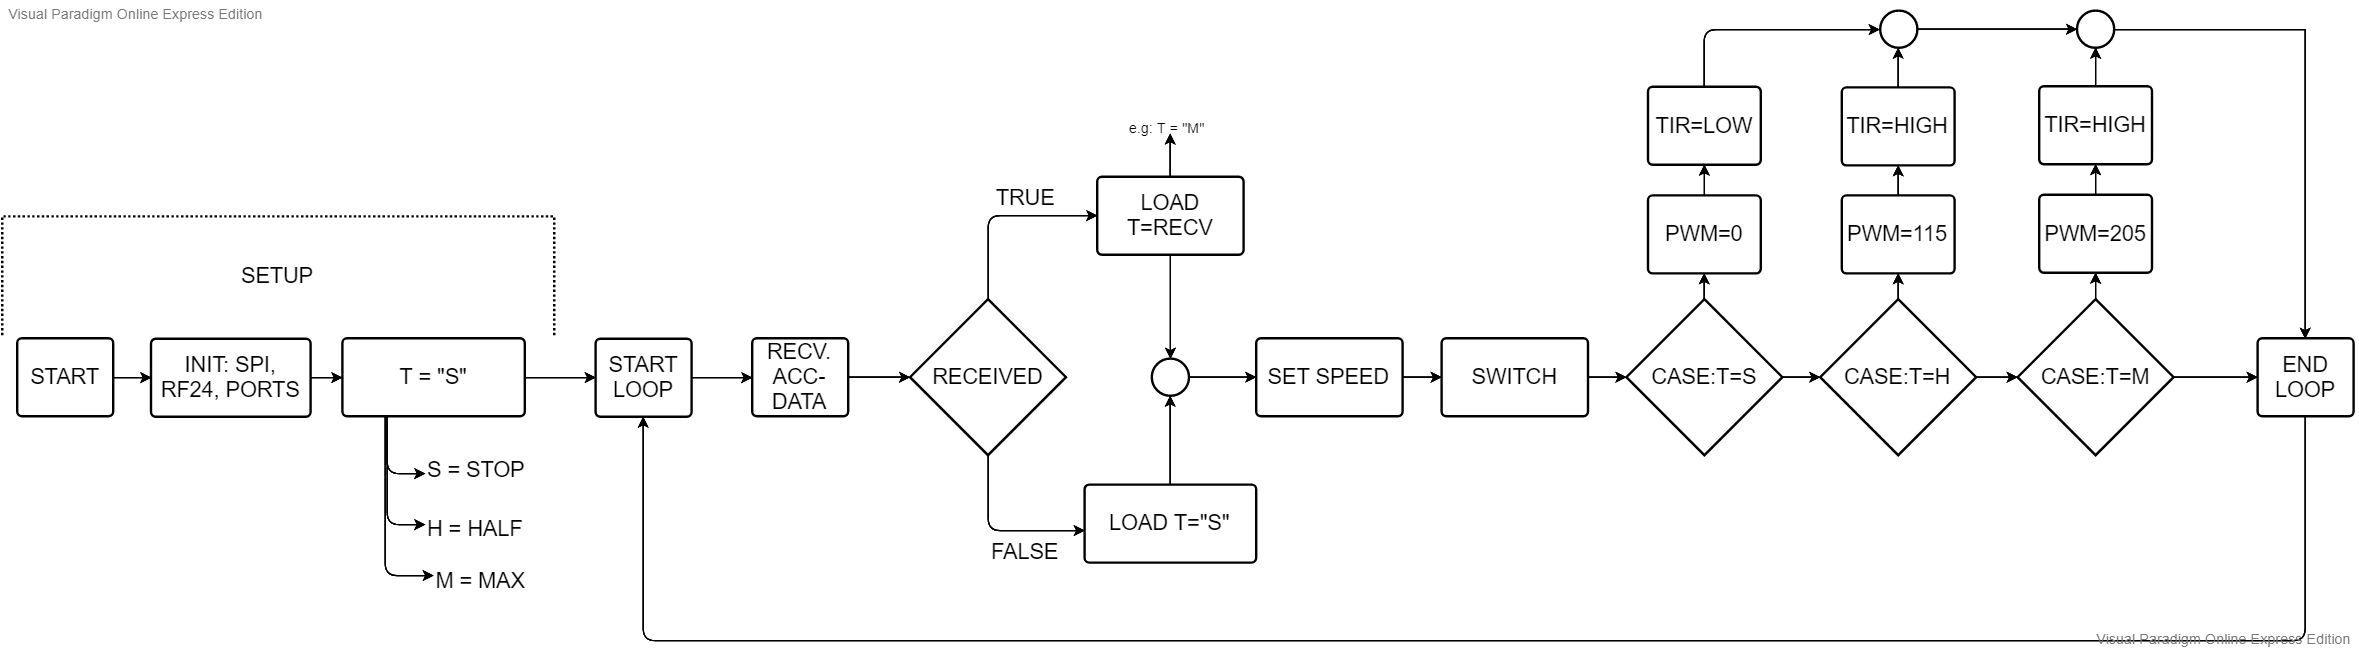
\includegraphics[width=\linewidth]{images/TM_module_flow_chart.png}
    \caption[TM folyamat ábra]{TM szoftver folyamat ábra}
	\label{fig:TMflowchart}
\end{figure}

\subsubsection{Észlelő hálózat}\subsubsectionro{Rețeaua de detectare}
A VM a blokkokat két típusú állapottal jellemzi.
\begin{enumerate}
	\item \textbf{'O' - OCCUPIED} - A specifikus blokk foglalt 
	\item \textbf{'F' - FREE} - A specifikus blokk szabad
\end{enumerate}

A VM hálózati információt egy  \mintinline{cpp}{char vacancy[8]} \mintinline{cpp}{ = FFFFFFFF} típusú pufferben tároljuk. Mivel 8 tervezett blokk van a rendszerben, ezért a puffer méret is ennek megfelel.
A puffer mindegyik indexéhez egy blokkot rendelünk, és az indexen található karakter leírja a blokk foglaltsági állapotát.
A VM hálózatban a 8 darab elhelyezett LDR szenzor a következő módon olvassa be a szenzor adatokat:

\begin{lstlisting}[style=CStyle, caption={LDR adat beolvasása a VM hálózatban},label=code:vm_ldrin]
  // read inputs
  for (int i = 0; i < block_num; i++) {
    inputState[i] = analogRead(photoIn[i]);
  }
\end{lstlisting}

A \mintinline{cpp}{analogRead(photoIn[i])} függvény a 8 \mintinline{cpp}{INPUT} módra állított portról olvassa be az aktuális szenzor adatot.
Amikor a szenzor TIP jelet kap, első impulzusként kezeli, ekkor a pufferben a megfelelő indexet O-ra állítja, azaz foglalt blokk.
Vissza F-re csak akkor állítjuk amikor a soron következő blokk is megkapja a TIP jelet. Ekkor természetesen a következő blokk állapota kerül O-ra.
Ily módon lefedjük a blokkszenzorok közötti átmenetet. 
Mivel a fizikai távolság miatt, megtörténhet hogy a mozdony TIP komponense elhagyja a blokk szenzort, viszont még nem érte el a következő blokk szenzort, és a rendszer ismeretlen állapotba kerülhet.
Az az egy rövid ideig úgy tűnne hogy a mozdony eltűnik a hálózatból.

Éppen ezért mindegyik blokkban egy állapot ledet is helyeztünk el, amely a fenti algoritmusra reagál.
Tehát amíg az állapot LED aktív a blokk foglalt állapotban marad. 
Végül pedig az összegyűjtött adatot, karakter tömbbe csomagolva, továbbítja a VM az ACC-nek.

A VM-ben lefutó program folyamat ábrát láthatjuk a \ref{fig:VMflowchart}. ábrán.

\begin{figure}[!htp]
	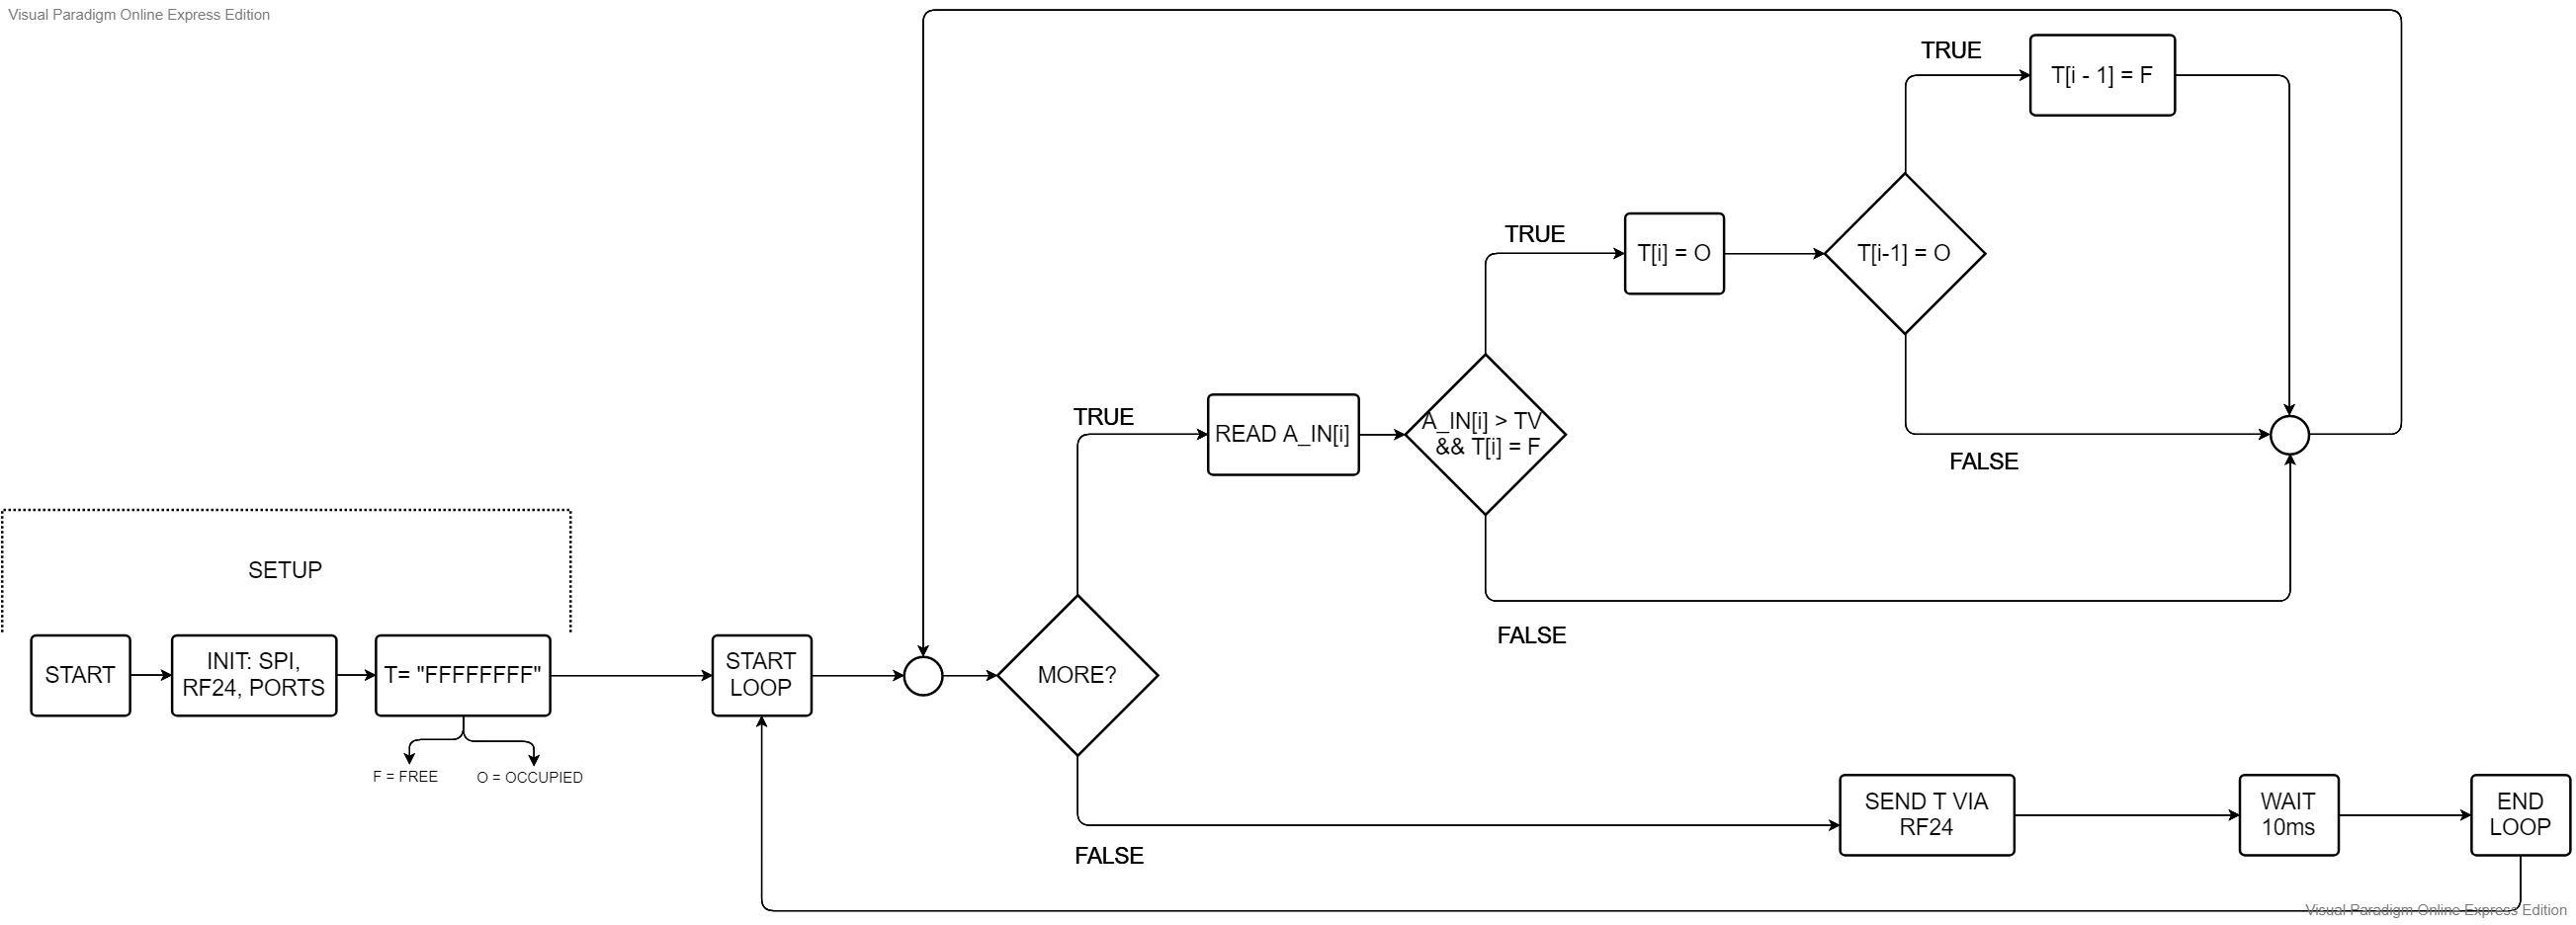
\includegraphics[width=\linewidth]{images/VM_module_flow_chart.png}
    \caption[VM folyamat ábra]{VM szoftver folyamat ábra}
	\label{fig:VMflowchart}
\end{figure}

\subsubsection{Jelző hálózat}\subsubsectionro{Rețeaua de semnalizare}
Az SM a blokkokat három típusú állapottal jelmezi.
\begin{enumerate}
	\item \textbf{'R' - RED} - Az aktuális blokk foglalt behajtani szigorúan tilós
	\item \textbf{'Y' - YELLOW} - Az aktuális blokkot követő blokk foglalt, behajtani figyelemmel és csökkentett sebességgel
	\item \textbf{'G' - GREEN} - Az aktuális blokk szabad, behajtani engedélyezett maximális sebességgel
\end{enumerate}
Továbbá az SM ugyancsak egy blokkok számának megfelelő 8 méretű puffer adatot kap az ACC-től az RFC-n keresztül.
Ezt szoftverileg így valósítjuk meg: \mintinline{cpp}{char signal[8]} \mintinline{cpp}{ = RYGGRYGG}. 
Az SM-ben található shift regiszterek természetesen ezt az adatot nem tudják értelmezni, éppen ezért szükséges egy konverzió alkalmazása.
Továbbá mint látható 8 adat érkezik, mindegyik blokknak egy érvényes aspektus. 
Ezt az adatot felhasználva szükséges a regiszterek 24 darab kimeneti portját aktiválni.
Az alkalmazott logika a \ref{tab:registercoding}. táblázatban leírt szabályok szerint történik.
Tehát egy blokknak három lehetséges aspektusa lehet, éppen ezért mindegyik blokknak megfeleltetünk három regiszter kimeneti portot.
Nyilván ezekből mindig csak egyik lehet aktív, ez azt jelenti hogy például  \mintinline{cpp}{R} esetén, az \mintinline{cpp}{R} portra egy \mintinline{cpp}{1}-es bitet valamint a másik két portra \mintinline{cpp}{0}-ás bitet írunk.
A táblázatot úgy kell értelmezni hogy az \mintinline{cpp}{1}-es blokk \mintinline{cpp}{R} aspektusának a vezérléséhez az \mintinline{cpp}{SR1} regiszter $Q_{0}$ portját szükséges manipulálni.

Ezt a szabály alkalmazva a beérkezett \mintinline{cpp}{char signal[8]} puffer tartalmát egyszer konvertáljuk egy \mintinline{cpp}{char fullstatelist[24]} típusú pufferben.
Aspektus és szabálytól függően 0-ást vagy 1-ear írva az új tárolóba:

\begin{table}[htp]
\centering
\begin{tabular}{|c|c|c|c|c|}
\hline
Blokk szám         & Aspektus & Aktív & Inaktív & Regiszter port \\ \hline
\multirow{3}{*}{1} & R        & 1     & 0       &\cellcolor{blue!25} $SR1_{Q_{0}}$  \\ \cline{2-5} 
                   & Y        & 1     & 0       &\cellcolor{blue!25} $SR1_{Q_{1}}$ \\ \cline{2-5} 
                   & G        & 1     & 0       &\cellcolor{blue!25} $SR1_{Q_{2}}$  \\ \hline
\multirow{3}{*}{2} & R        & 1     & 0       &\cellcolor{blue!25} $SR1_{Q_{3}}$  \\ \cline{2-5} 
                   & Y        & 1     & 0       &\cellcolor{blue!25} $SR1_{Q_{4}}$  \\ \cline{2-5} 
                   & G        & 1     & 0       &\cellcolor{blue!25} $SR1_{Q_{5}}$  \\ \hline
\multirow{3}{*}{3} & R        & 1     & 0       &\cellcolor{blue!25} $SR1_{Q_{6}}$  \\ \cline{2-5} 
                   & Y        & 1     & 0       &\cellcolor{blue!25} $SR1_{Q_{7}}$  \\ \cline{2-5} 
                   & G        & 1     & 0       & $SR2_{Q_{0}}$  \\ \hline
\multirow{3}{*}{4} & R        & 1     & 0       & $SR2_{Q_{1}}$  \\ \cline{2-5} 
                   & Y        & 1     & 0       & $SR2_{Q_{2}}$  \\ \cline{2-5} 
                   & G        & 1     & 0       & $SR2_{Q_{3}}$  \\ \hline
\multirow{3}{*}{5} & R        & 1     & 0       & $SR2_{Q_{4}}$  \\ \cline{2-5} 
                   & Y        & 1     & 0       & $SR2_{Q_{5}}$  \\ \cline{2-5} 
                   & G        & 1     & 0       & $SR2_{Q_{6}}$  \\ \hline
\multirow{3}{*}{6} & R        & 1     & 0       & $SR2_{Q_{7}}$  \\ \cline{2-5} 
                   & Y        & 1     & 0       &\cellcolor{blue!25} $SR3_{Q_{0}}$  \\ \cline{2-5} 
                   & G        & 1     & 0       &\cellcolor{blue!25} $SR3_{Q_{1}}$  \\ \hline
\multirow{3}{*}{7} & R        & 1     & 0       &\cellcolor{blue!25} $SR3_{Q_{2}}$  \\ \cline{2-5} 
                   & Y        & 1     & 0       &\cellcolor{blue!25} $SR3_{Q_{3}}$  \\ \cline{2-5} 
                   & G        & 1     & 0       &\cellcolor{blue!25} $SR3_{Q_{4}}$  \\ \hline
\multirow{3}{*}{8} & R        & 1     & 0       &\cellcolor{blue!25} $SR3_{Q_{5}}$  \\ \cline{2-5} 
                   & Y        & 1     & 0       &\cellcolor{blue!25} $SR3_{Q_{6}}$  \\ \cline{2-5} 
                   & G        & 1     & 0       &\cellcolor{blue!25} $SR3_{Q_{7}}$  \\ \hline
\end{tabular}
    \caption[Regiszter kódolás]{A shift regiszterek portjainak aktiválása}
    \label{tab:registercoding}
\end{table}

\begin{minipage}{\linewidth}
\begin{lstlisting}[style=CStyle, caption={Aspektus információ dekódolása a regiszterek számára},label=code:sm_decode_asp]
void decode_aspects_to_register() {
  int j = 0;
  for (int i = 0; i < sizeof(local_signal); i++) {
    switch (local_signal[i]) {
      case 'R':
        full_state_list[j] = 1;
        full_state_list[j + 1] = 0;
        full_state_list[j + 2] = 0;
        break;
      case 'Y':
        full_state_list[j] = 0;
        full_state_list[j + 1] = 1;
        full_state_list[j + 2] = 0;
        break;
      case 'G':
        full_state_list[j] = 0;
        full_state_list[j + 1] = 0;
        full_state_list[j + 2] = 1;
        break;
    }
    j = j + 3;
  }
}
\end{lstlisting}
\end{minipage}

Ezután a tárolót tartalmát felosszuk három kisebb tárolóra, ahova betöltjük a kész a regiszterek által értelmezhető információt.
A konkrét betöltés a regiszterekben egy \mintinline{cpp}{byte} típusú változó és az előkészített regiszter bejárásával valósítjuk meg.
Használva a beépített \mintinline{cpp}{ bitSet(byte, position)} függvényt amely 1-est ír a változó megfelelő bit pozíciójára.
Valamint a  \mintinline{cpp}{ bitClear(byte, position)} függvényt amely 0-ást ír.

A regisztereknek bekonfigurált portjai manipulálva pedig kitesszük a \mintinline{cpp}{byte} változóban tárolt biteket a regiszter kimeneteire.

\begin{lstlisting}[style=CStyle, caption={Shit regisztert aktiváló kód SM-ben},label=code:sm_shift_update]
//bring latch pin to low, put the byte data on the data pin, and pull latch back to high to shift it out
void updateShiftRegisters(){
	digitalWrite(s1_latch, LOW);
	shiftOut(s1_data, s1_clock, MSBFIRST, aspects_sr_1);
	digitalWrite(s1_latch, HIGH);
}
\end{lstlisting}

Az \mintinline{cpp}{s1clock} változó a shift regiszter \textit{SHCP} órajelportját vezérli, amely beiráskor aktiv. 
Az \mintinline{cpp}{s1data} változó a shift regiszter \textit{DS} soros adat bemeneti portját képviseli.
Ez a kettő mellet természetsen a \mintinline{cpp}{shiftOut()} függvénynek átadjuk a beírandó byte-nyi adatot is, ez kerül beírásra a regiszter pufferébe.
Végül az \mintinline{cpp}{s1latch} változón keresztül a shift regiszter \textit{STCP} portra ha felmenő órajelet küldünk, a regiszterben tárolt adatot, a regiszter kiküldi a kimeneti portjaira. 
Így aktiválva a megfelelő LED-et az SM hálózatban.

Az SM-ben lefutó program folyamat diagramot láthatjuk a \ref{fig:SMflowchart}. ábrán.

\begin{figure}[!htp]
	\includegraphics[width=\linewidth]{images/SM_module_flow_chart.png}
    \caption[SM folyamat ábra]{SM szoftver folyamat ábra}
	\label{fig:SMflowchart}
\end{figure}

\subsubsection{Központi vezérlő modúl}\subsubsectionro{Modulul central de control}
Az ACC ügynökként viselkedik, ahogy a kommunikációs fejezetben már említettük.
Lényegében a kommunikációs feladatain kívül egy pár tároló menedzselésével foglalkozik egy jól meghatározott algoritmus szerint.
A tárgyalt modulok szerinti tárolók pedig a következőek:

\begin{minipage}{\linewidth}
\begin{lstlisting}[style=CStyle, caption={Tárolok inicializálása az ACC-ben},label=code:acc_array_init]
const int train_num = 2
const int data_size = 8
char central_signal[data_size] = XXXXXXXX
char central_vacancy[data_size] = FFFFFFFF
char central_train[train_num] = SS
\end{lstlisting}
\end{minipage}

A \mintinline{cpp}{dataSize} egyenlő a blokkok számával.
A jelző és észlelő adat tárolók pedig, itt, az implicit indulási értékeket tartalmazzák.
A TM adat \mintinline{cpp}{S} karaktere az alap megállási állapotot írja le.
A VM adat \mintinline{cpp}{F} karaktere az üres hálózatot jellemzi amikor az összes blokk szabad.
Végül az SM adat \mintinline{cpp}{X} karaktere \textit{Default}  állapotot jelent, és ez csak kezdetkor és újra számoláskor marad így.
Mivel \mintinline{cpp}{X} aspektus nem létezik, ez a programozásban ismert bármilyen állapot jellemzi.
Mi esetünkben termesztésen az értelmezendő pufferben nem lehet csak az alap értelmezett 3 aspektus.
Tehát ez az állapot mindig \mintinline{cpp}{G} aspektust fog jelenteni, azaz mivel egyik szomszédos blokkja sem foglalt a behajtás engedélyezett.
Ezt a feladatot, valamint a rendszer biztonságát garantáló aspektus számítást, az úgy nevezett \textbf{SIAS - Signal Aspect Sequencing} algoritmus végzi el.
Az algoritmus bemenetként mindig a vonatok számát valamint a VM-től érkezett és centralVacancy pufferbe betöltött hálózati jelenlét adatok képezik.
A hálózatban található vonatok számát az ACC is inicializálja, de a számításokhoz a VM pufferben található \mintinline{cpp}{O} állapotok számát használjuk:

\begin{minipage}{\linewidth}
\begin{lstlisting}[style=CStyle, caption={Mozdonyok számának meghatározása észlelési adatok alapján},label=code:acc_train_num]
//central_train buffer can be inaccurate, field sensor input is considered more valid, so based on it we calculate the number of trains in the network
int count_train() {
  int val = 0;
  for ( int i = 0; i < data_size; i++) {
    if (central_vacancy[i] == 'O')
      val++;
  }
  return val;
}
\end{lstlisting}
\end{minipage}

Ez azért szükséges mert ha véletlenül az ACC hibás adatokkal rendelkezik, a szenzorok által szolgáltatott információ biztosabbnak tekinthető.
Az algoritmusnak tehát két lehetséges lefutási esete van. A hálózatban egy vagy két vonat van jelen. 
Az algoritmus kezdetben azonosítja ezt a fentebb említett függvény segítségével.
Továbbá egy másik kezdeti feltétel a jelenleg a jelző tárolóban található aspektusok visszaállításra az alap állapotra.

\begin{minipage}{\linewidth}
\begin{lstlisting}[style=CStyle, caption={Alap állapotok beállítása az ACC-ben},label=code:acc_sig_def]
 //loop through vacancy array and set signal aspects according to Occupied blocks
 for ( int i = 0; i < data_size; i++) {
   central_signal[i] = 'X';
 }
\end{lstlisting}
\end{minipage}

Ez egy biztonsági lépés, ami alapján az aspektusokat mindig az új észlelési adatok alapján számoljuk, így nem befolyásolhatnak hibásan a korábbi iterációban meghatározott aspektusok.
Az ACC-ben lefutó program folyamat ábrát láthatjuk a \ref{fig:ACCflowchart}. ábrán.

\begin{figure}[!htp]
	\includegraphics[width=\linewidth]{images/ACC_module_flow_chart.png}
    \caption[ACC folyamat ábra]{ACC szoftver folyamat ábra}
	\label{fig:ACCflowchart}
\end{figure}


Maga algoritmus lényegében két kör puffer követéséhez és frissítéséhez hasonlít. 
A VM puffer azon pozíciójában ahol \mintinline{cpp}{O} állapotot találunk az SM puffer megfelelő pozíciójában \mintinline{cpp}{R} aspektust, a jobbra szomszédban \mintinline{cpp}{Y} aspektust, végül a balra szomszédban \mintinline{cpp}{G} aspektust állitunk be.
Egy vonat esetén a hálózatban az algoritmus a \ref{tab:sias_onetrain}. táblázatban leírtak szerint fog alakulni.

\begin{table}[htp]
\centering
\begin{tabular}{lllllllll}
\hline
\multicolumn{1}{|l|}{Block} & \multicolumn{1}{l|}{0}                         & \multicolumn{1}{l|}{1}                         & \multicolumn{1}{l|}{2}                         & \multicolumn{1}{l|}{3}                         & \multicolumn{1}{l|}{4}                         & \multicolumn{1}{l|}{5}                         & \multicolumn{1}{l|}{6}                                                & \multicolumn{1}{l|}{7}                                                \\ \hline
\multicolumn{1}{|l|}{DET.}  & \multicolumn{1}{l|}{\cellcolor[HTML]{FD6864}O} & \multicolumn{1}{l|}{\cellcolor[HTML]{32CB00}F} & \multicolumn{1}{l|}{\cellcolor[HTML]{32CB00}F} & \multicolumn{1}{l|}{\cellcolor[HTML]{32CB00}F} & \multicolumn{1}{l|}{\cellcolor[HTML]{32CB00}F} & \multicolumn{1}{l|}{\cellcolor[HTML]{32CB00}F} & \multicolumn{1}{l|}{\cellcolor[HTML]{32CB00}F}                        & \multicolumn{1}{l|}{\cellcolor[HTML]{32CB00}F}                        \\ \hline
\multicolumn{1}{|l|}{ASP.}  & \multicolumn{1}{l|}{\cellcolor[HTML]{FE0000}R} & \multicolumn{1}{l|}{\cellcolor[HTML]{009901}G} & \multicolumn{1}{l|}{X}                         & \multicolumn{1}{l|}{X}                         & \multicolumn{1}{l|}{X}                         & \multicolumn{1}{l|}{X}                         & \multicolumn{1}{l|}{X}                                                & \multicolumn{1}{l|}{\cellcolor[HTML]{F8FF00}Y}                        \\ \hline
                            &                                                &                                                &                                                &                                                &                                                &                                                &                                                                       &                                                                       \\ \hline
\multicolumn{1}{|l|}{VAC}   & \multicolumn{1}{l|}{\cellcolor[HTML]{32CB00}F} & \multicolumn{1}{l|}{\cellcolor[HTML]{FD6864}O} & \multicolumn{1}{l|}{\cellcolor[HTML]{32CB00}F} & \multicolumn{1}{l|}{\cellcolor[HTML]{32CB00}F} & \multicolumn{1}{l|}{\cellcolor[HTML]{32CB00}F} & \multicolumn{1}{l|}{\cellcolor[HTML]{32CB00}F} & \multicolumn{1}{l|}{\cellcolor[HTML]{32CB00}F}                        & \multicolumn{1}{l|}{\cellcolor[HTML]{32CB00}F}                        \\ \hline
\multicolumn{1}{|l|}{SIG}   & \multicolumn{1}{l|}{\cellcolor[HTML]{F8FF00}Y} & \multicolumn{1}{l|}{\cellcolor[HTML]{FE0000}R} & \multicolumn{1}{l|}{\cellcolor[HTML]{009901}G} & \multicolumn{1}{l|}{X}                         & \multicolumn{1}{l|}{X}                         & \multicolumn{1}{l|}{X}                         & \multicolumn{1}{l|}{X}                                                & \multicolumn{1}{l|}{X}                                                \\ \hline
                            &                                                &                                                &                                                &                                                &                                                &                                                &                                                                       &                                                                       \\ \hline
\multicolumn{1}{|l|}{VAC}   & \multicolumn{1}{l|}{\cellcolor[HTML]{32CB00}F} & \multicolumn{1}{l|}{\cellcolor[HTML]{32CB00}F} & \multicolumn{1}{l|}{\cellcolor[HTML]{FD6864}O} & \multicolumn{1}{l|}{\cellcolor[HTML]{32CB00}F} & \multicolumn{1}{l|}{\cellcolor[HTML]{32CB00}F} & \multicolumn{1}{l|}{\cellcolor[HTML]{32CB00}F} & \multicolumn{1}{l|}{\cellcolor[HTML]{32CB00}F}                        & \multicolumn{1}{l|}{\cellcolor[HTML]{32CB00}F}                        \\ \hline
\multicolumn{1}{|l|}{SIG}   & \multicolumn{1}{l|}{X}                         & \multicolumn{1}{l|}{\cellcolor[HTML]{F8FF00}Y} & \multicolumn{1}{l|}{\cellcolor[HTML]{FE0000}R} & \multicolumn{1}{l|}{\cellcolor[HTML]{009901}G} & \multicolumn{1}{l|}{X}                         & \multicolumn{1}{l|}{X}                         & \multicolumn{1}{l|}{X}                                                & \multicolumn{1}{l|}{X}                                                \\ \hline
                            &                                                &                                                &                                                &                                                &                                                &                                                &                                                                       &                                                                       \\ \hline
\multicolumn{1}{|l|}{VAC}   & \multicolumn{1}{l|}{\cellcolor[HTML]{32CB00}F} & \multicolumn{1}{l|}{\cellcolor[HTML]{32CB00}F} & \multicolumn{1}{l|}{\cellcolor[HTML]{32CB00}F} & \multicolumn{1}{l|}{\cellcolor[HTML]{FD6864}O} & \multicolumn{1}{l|}{\cellcolor[HTML]{32CB00}F} & \multicolumn{1}{l|}{\cellcolor[HTML]{32CB00}F} & \multicolumn{1}{l|}{\cellcolor[HTML]{32CB00}F}                        & \multicolumn{1}{l|}{\cellcolor[HTML]{32CB00}F}                        \\ \hline
\multicolumn{1}{|l|}{SIG}   & \multicolumn{1}{l|}{X}                         & \multicolumn{1}{l|}{X}                         & \multicolumn{1}{l|}{\cellcolor[HTML]{F8FF00}Y} & \multicolumn{1}{l|}{\cellcolor[HTML]{FE0000}R} & \multicolumn{1}{l|}{\cellcolor[HTML]{009901}G} & \multicolumn{1}{l|}{X}                         & \multicolumn{1}{l|}{X}                                                & \multicolumn{1}{l|}{X}                                                \\ \hline
                            &                                                &                                                &                                                &                                                &                                                &                                                &                                                                       &                                                                       \\ \hline
\multicolumn{1}{|l|}{VAC}   & \multicolumn{1}{l|}{\cellcolor[HTML]{32CB00}F} & \multicolumn{1}{l|}{\cellcolor[HTML]{32CB00}F} & \multicolumn{1}{l|}{\cellcolor[HTML]{32CB00}F} & \multicolumn{1}{l|}{\cellcolor[HTML]{32CB00}F} & \multicolumn{1}{l|}{\cellcolor[HTML]{FD6864}O} & \multicolumn{1}{l|}{\cellcolor[HTML]{32CB00}F} & \multicolumn{1}{l|}{\cellcolor[HTML]{32CB00}F}                        & \multicolumn{1}{l|}{\cellcolor[HTML]{32CB00}F}                        \\ \hline
\multicolumn{1}{|l|}{SIG}   & \multicolumn{1}{l|}{X}                         & \multicolumn{1}{l|}{Y}                         & \multicolumn{1}{l|}{X}                         & \multicolumn{1}{l|}{\cellcolor[HTML]{F8FF00}Y} & \multicolumn{1}{l|}{\cellcolor[HTML]{FE0000}R} & \multicolumn{1}{l|}{\cellcolor[HTML]{009901}G} & \multicolumn{1}{l|}{X}                                                & \multicolumn{1}{l|}{X}                                                \\ \hline
                            &                                                &                                                &                                                &                                                &                                                &                                                &                                                                       &                                                                       \\ \hline
\multicolumn{1}{|l|}{VAC}   & \multicolumn{1}{l|}{\cellcolor[HTML]{32CB00}F} & \multicolumn{1}{l|}{\cellcolor[HTML]{32CB00}F} & \multicolumn{1}{l|}{\cellcolor[HTML]{32CB00}F} & \multicolumn{1}{l|}{\cellcolor[HTML]{32CB00}F} & \multicolumn{1}{l|}{\cellcolor[HTML]{32CB00}F} & \multicolumn{1}{l|}{\cellcolor[HTML]{FD6864}O} & \multicolumn{1}{l|}{\cellcolor[HTML]{32CB00}{\color[HTML]{000000} F}} & \multicolumn{1}{l|}{\cellcolor[HTML]{32CB00}{\color[HTML]{000000} F}} \\ \hline
\multicolumn{1}{|l|}{SIG}   & \multicolumn{1}{l|}{X}                         & \multicolumn{1}{l|}{X}                         & \multicolumn{1}{l|}{X}                         & \multicolumn{1}{l|}{X}                         & \multicolumn{1}{l|}{\cellcolor[HTML]{F8FF00}Y} & \multicolumn{1}{l|}{\cellcolor[HTML]{FE0000}R} & \multicolumn{1}{l|}{\cellcolor[HTML]{009901}G}                        & \multicolumn{1}{l|}{X}                                                \\ \hline
                            &                                                &                                                &                                                &                                                &                                                &                                                &                                                                       &                                                                       \\ \hline
\multicolumn{1}{|l|}{VAC}   & \multicolumn{1}{l|}{\cellcolor[HTML]{32CB00}F} & \multicolumn{1}{l|}{\cellcolor[HTML]{32CB00}F} & \multicolumn{1}{l|}{\cellcolor[HTML]{32CB00}F} & \multicolumn{1}{l|}{\cellcolor[HTML]{32CB00}F} & \multicolumn{1}{l|}{\cellcolor[HTML]{32CB00}F} & \multicolumn{1}{l|}{\cellcolor[HTML]{32CB00}F} & \multicolumn{1}{l|}{\cellcolor[HTML]{FD6864}O}                        & \multicolumn{1}{l|}{\cellcolor[HTML]{32CB00}F}                        \\ \hline
\multicolumn{1}{|l|}{SIG}   & \multicolumn{1}{l|}{X}                         & \multicolumn{1}{l|}{X}                         & \multicolumn{1}{l|}{X}                         & \multicolumn{1}{l|}{X}                         & \multicolumn{1}{l|}{X}                         & \multicolumn{1}{l|}{\cellcolor[HTML]{F8FF00}Y} & \multicolumn{1}{l|}{\cellcolor[HTML]{FE0000}R}                        & \multicolumn{1}{l|}{\cellcolor[HTML]{009901}G}                        \\ \hline
                            &                                                &                                                &                                                &                                                &                                                &                                                &                                                                       &                                                                       \\ \hline
\multicolumn{1}{|l|}{VAC}   & \multicolumn{1}{l|}{\cellcolor[HTML]{32CB00}F} & \multicolumn{1}{l|}{\cellcolor[HTML]{32CB00}F} & \multicolumn{1}{l|}{\cellcolor[HTML]{32CB00}F} & \multicolumn{1}{l|}{\cellcolor[HTML]{32CB00}F} & \multicolumn{1}{l|}{\cellcolor[HTML]{32CB00}F} & \multicolumn{1}{l|}{\cellcolor[HTML]{32CB00}F} & \multicolumn{1}{l|}{\cellcolor[HTML]{32CB00}F}                        & \multicolumn{1}{l|}{\cellcolor[HTML]{FD6864}O}                        \\ \hline
\multicolumn{1}{|l|}{SIG}   & \multicolumn{1}{l|}{\cellcolor[HTML]{009901}G} & \multicolumn{1}{l|}{X}                         & \multicolumn{1}{l|}{X}                         & \multicolumn{1}{l|}{X}                         & \multicolumn{1}{l|}{X}                         & \multicolumn{1}{l|}{X}                         & \multicolumn{1}{l|}{\cellcolor[HTML]{F8FF00}Y}                        & \multicolumn{1}{l|}{\cellcolor[HTML]{FE0000}R}                        \\ \hline
\end{tabular}
\caption[SIAS 1 mozdonnyal]{Jelző aspektus számolás a blokk hálózatban egy mozdony esetén}
\label{tab:sias_onetrain}
\end{table}

Maga a kód amely megvalósítja:

\begin{minipage}{\linewidth}
\begin{lstlisting}[style=CStyle, caption={SIAS algoritmus, egy vonat esettén az ACC-ben},label=code:acc_sias_1]
// value to hold overflow of circular buffer boundry
int end_ar = 0;
//loop through vacancy array and set signal aspects according to Occupied blocks
for ( int i = 0; i < data_size; i++) {
	if (t == 1 && central_vacancy[i % data_size] == 'O')  {
      central_signal[i % data_size] = 'R';
      central_signal[(i + 1) % data_size] = 'G';
      if ( i - 1 < 0) {
        central_signal[end_ar] = 'Y';
      } else {
        central_signal[(i - 1) % data_size] = 'Y';
      }
      // issue SPEED_MAX command
	  char centralTrain[trainNum] = MS
    }
}
\end{lstlisting}
\end{minipage}
És végül az algoritmus logika folyamat ábrája látható a \ref{fig:SIAS1flowchart}. ábrán.

\begin{figure}[!htp]
	\includegraphics[width=\linewidth]{images/SIAS1_module_flow_chart.png}
    \caption[SIAS 1 folyamat ábra]{SIAS 1 algoritmus folyamat ábra}
	\label{fig:SIAS1flowchart}
\end{figure}

Két vonat esetén is hasonló elvet alkalmazunk viszont ebben az esetben potenciális konfliktusok alakulhatnak ki amikor a két mozdony túl közel kerül egymáshoz.
Ezt az algoritmus úgy kezeli le hogy a menet iránytól felfele tartózkodó mozdonynak prioritása van, és az ő aspektusait, a hátulról érkező mozdony nem írhatja felül.
Ennek egy példáját látjuk lejátszódni a \ref{tab:sias_2trains}. táblázatban. 
Egy további biztonsági implementációt a konfliktusok esetén alkalmaztam.
Ha a vonat nem módosítja sebességét az aspektusnak megfelelően, az algoritmus automatikusan felül írja a felhasználó által beállított sebességet, és továbbítja a TM-nek végrehajtásra.

\begin{table}[htp]
\centering
\begin{tabular}{lllllllll}
\hline
\multicolumn{1}{|l|}{Block} & \multicolumn{1}{l|}{0}                         & \multicolumn{1}{l|}{1}                         & \multicolumn{1}{l|}{2}                                                & \multicolumn{1}{l|}{3}                                                & \multicolumn{1}{l|}{4}                         & \multicolumn{1}{l|}{5}                         & \multicolumn{1}{l|}{6}                                                & \multicolumn{1}{l|}{7}                                                \\ \hline
\multicolumn{1}{|l|}{DET.}  & \multicolumn{1}{l|}{\cellcolor[HTML]{FD6864}O} & \multicolumn{1}{l|}{\cellcolor[HTML]{32CB00}F} & \multicolumn{1}{l|}{\cellcolor[HTML]{32CB00}F}                        & \multicolumn{1}{l|}{\cellcolor[HTML]{32CB00}F}                        & \multicolumn{1}{l|}{\cellcolor[HTML]{32CB00}F} & \multicolumn{1}{l|}{\cellcolor[HTML]{FD6864}O} & \multicolumn{1}{l|}{\cellcolor[HTML]{32CB00}F}                        & \multicolumn{1}{l|}{\cellcolor[HTML]{32CB00}F}                        \\ \hline
\multicolumn{1}{|l|}{ASP.}  & \multicolumn{1}{l|}{\cellcolor[HTML]{FE0000}R} & \multicolumn{1}{l|}{\cellcolor[HTML]{009901}G} & \multicolumn{1}{l|}{X}                                                & \multicolumn{1}{l|}{X}                                                & \multicolumn{1}{l|}{\cellcolor[HTML]{F8FF00}Y} & \multicolumn{1}{l|}{\cellcolor[HTML]{FE0000}R} & \multicolumn{1}{l|}{\cellcolor[HTML]{009901}G}                        & \multicolumn{1}{l|}{\cellcolor[HTML]{F8FF00}Y}                        \\ \hline
                            &                                                &                                                &                                                                       &                                                                       &                                                &                                                &                                                                       &                                                                       \\ \hline
\multicolumn{1}{|l|}{DET.}  & \multicolumn{1}{l|}{\cellcolor[HTML]{32CB00}F} & \multicolumn{1}{l|}{\cellcolor[HTML]{FD6864}O} & \multicolumn{1}{l|}{\cellcolor[HTML]{32CB00}F}                        & \multicolumn{1}{l|}{\cellcolor[HTML]{32CB00}F}                        & \multicolumn{1}{l|}{\cellcolor[HTML]{32CB00}F} & \multicolumn{1}{l|}{\cellcolor[HTML]{FD6864}O} & \multicolumn{1}{l|}{\cellcolor[HTML]{32CB00}F}                        & \multicolumn{1}{l|}{\cellcolor[HTML]{32CB00}F}                        \\ \hline
\multicolumn{1}{|l|}{ASP.}  & \multicolumn{1}{l|}{\cellcolor[HTML]{F8FF00}Y} & \multicolumn{1}{l|}{\cellcolor[HTML]{FE0000}R} & \multicolumn{1}{l|}{\cellcolor[HTML]{009901}G}                        & \multicolumn{1}{l|}{X}                                                & \multicolumn{1}{l|}{\cellcolor[HTML]{F8FF00}Y} & \multicolumn{1}{l|}{\cellcolor[HTML]{FE0000}R} & \multicolumn{1}{l|}{\cellcolor[HTML]{009901}G}                        & \multicolumn{1}{l|}{X}                                                \\ \hline
                            &                                                &                                                &                                                                       &                                                                       &                                                &                                                &                                                                       &                                                                       \\ \hline
\multicolumn{1}{|l|}{VAC}   & \multicolumn{1}{l|}{\cellcolor[HTML]{32CB00}F} & \multicolumn{1}{l|}{\cellcolor[HTML]{32CB00}F} & \multicolumn{1}{l|}{\cellcolor[HTML]{FD6864}O}                        & \multicolumn{1}{l|}{\cellcolor[HTML]{32CB00}F}                        & \multicolumn{1}{l|}{\cellcolor[HTML]{32CB00}F} & \multicolumn{1}{l|}{\cellcolor[HTML]{FD6864}O} & \multicolumn{1}{l|}{\cellcolor[HTML]{32CB00}F}                        & \multicolumn{1}{l|}{\cellcolor[HTML]{32CB00}F}                        \\ \hline
\multicolumn{1}{|l|}{SIG}   & \multicolumn{1}{l|}{X}                         & \multicolumn{1}{l|}{\cellcolor[HTML]{F8FF00}Y} & \multicolumn{1}{l|}{\cellcolor[HTML]{FE0000}R}                        & \multicolumn{1}{l|}{\cellcolor[HTML]{009901}G}                        & \multicolumn{1}{l|}{\cellcolor[HTML]{F8FF00}Y} & \multicolumn{1}{l|}{\cellcolor[HTML]{FE0000}R} & \multicolumn{1}{l|}{\cellcolor[HTML]{009901}{\color[HTML]{000000} G}} & \multicolumn{1}{l|}{X}                                                \\ \hline
                            &                                                &                                                &                                                                       &                                                                       &                                                &                                                &                                                                       &                                                                       \\ \hline
\multicolumn{1}{|l|}{VAC}   & \multicolumn{1}{l|}{\cellcolor[HTML]{32CB00}F} & \multicolumn{1}{l|}{\cellcolor[HTML]{32CB00}F} & \multicolumn{1}{l|}{\cellcolor[HTML]{32CB00}F}                        & \multicolumn{1}{l|}{\cellcolor[HTML]{FD6864}O}                        & \multicolumn{1}{l|}{\cellcolor[HTML]{32CB00}F} & \multicolumn{1}{l|}{\cellcolor[HTML]{FD6864}O} & \multicolumn{1}{l|}{\cellcolor[HTML]{32CB00}F}                        & \multicolumn{1}{l|}{\cellcolor[HTML]{32CB00}F}                        \\ \hline
\multicolumn{1}{|l|}{SIG}   & \multicolumn{1}{l|}{X}                         & \multicolumn{1}{l|}{X}                         & \multicolumn{1}{l|}{\cellcolor[HTML]{F8FF00}Y}                        & \multicolumn{1}{l|}{\cellcolor[HTML]{FE0000}R}                        & \multicolumn{1}{l|}{\cellcolor[HTML]{F8FF00}Y} & \multicolumn{1}{l|}{\cellcolor[HTML]{FE0000}R} & \multicolumn{1}{l|}{\cellcolor[HTML]{009901}G}                        & \multicolumn{1}{l|}{X}                                                \\ \hline
                            &                                                &                                                &                                                                       &                                                                       &                                                &                                                &                                                                       &                                                                       \\ \hline
\multicolumn{1}{|l|}{VAC}   & \multicolumn{1}{l|}{\cellcolor[HTML]{32CB00}F} & \multicolumn{1}{l|}{\cellcolor[HTML]{32CB00}F} & \multicolumn{1}{l|}{\cellcolor[HTML]{32CB00}F}                        & \multicolumn{1}{l|}{\cellcolor[HTML]{32CB00}F}                        & \multicolumn{1}{l|}{\cellcolor[HTML]{FD6864}O} & \multicolumn{1}{l|}{\cellcolor[HTML]{FD6864}O} & \multicolumn{1}{l|}{\cellcolor[HTML]{32CB00}F}                        & \multicolumn{1}{l|}{\cellcolor[HTML]{32CB00}F}                        \\ \hline
\multicolumn{1}{|l|}{SIG}   & \multicolumn{1}{l|}{X}                         & \multicolumn{1}{l|}{Y}                         & \multicolumn{1}{l|}{X}                                                & \multicolumn{1}{l|}{\cellcolor[HTML]{F8FF00}Y}                        & \multicolumn{1}{l|}{\cellcolor[HTML]{FE0000}R} & \multicolumn{1}{l|}{\cellcolor[HTML]{FE0000}R} & \multicolumn{1}{l|}{\cellcolor[HTML]{009901}G}                        & \multicolumn{1}{l|}{X}                                                \\ \hline
                            &                                                &                                                &                                                                       &                                                                       &                                                &                                                &                                                                       &                                                                       \\ \hline
\multicolumn{1}{|l|}{VAC}   & \multicolumn{1}{l|}{\cellcolor[HTML]{32CB00}F} & \multicolumn{1}{l|}{\cellcolor[HTML]{32CB00}F} & \multicolumn{1}{l|}{\cellcolor[HTML]{32CB00}F}                        & \multicolumn{1}{l|}{\cellcolor[HTML]{32CB00}F}                        & \multicolumn{1}{l|}{\cellcolor[HTML]{32CB00}F} & \multicolumn{1}{l|}{\cellcolor[HTML]{FD6864}O} & \multicolumn{1}{l|}{\cellcolor[HTML]{32CB00}{\color[HTML]{000000} F}} & \multicolumn{1}{l|}{\cellcolor[HTML]{FD6864}{\color[HTML]{000000} O}} \\ \hline
\multicolumn{1}{|l|}{SIG}   & \multicolumn{1}{l|}{\cellcolor[HTML]{009901}G} & \multicolumn{1}{l|}{X}                         & \multicolumn{1}{l|}{X}                                                & \multicolumn{1}{l|}{X}                                                & \multicolumn{1}{l|}{\cellcolor[HTML]{F8FF00}Y} & \multicolumn{1}{l|}{\cellcolor[HTML]{FE0000}R} & \multicolumn{1}{l|}{\cellcolor[HTML]{F8FF00}Y}                        & \multicolumn{1}{l|}{\cellcolor[HTML]{FE0000}R}                        \\ \hline
                            &                                                &                                                &                                                                       &                                                                       &                                                &                                                &                                                                       &                                                                       \\ \hline
\multicolumn{1}{|l|}{VAC}   & \multicolumn{1}{l|}{\cellcolor[HTML]{32CB00}F} & \multicolumn{1}{l|}{\cellcolor[HTML]{FD6864}O} & \multicolumn{1}{l|}{\cellcolor[HTML]{32CB00}F}                        & \multicolumn{1}{l|}{\cellcolor[HTML]{32CB00}F}                        & \multicolumn{1}{l|}{\cellcolor[HTML]{32CB00}F} & \multicolumn{1}{l|}{\cellcolor[HTML]{32CB00}F} & \multicolumn{1}{l|}{\cellcolor[HTML]{FD6864}O}                        & \multicolumn{1}{l|}{\cellcolor[HTML]{32CB00}F}                        \\ \hline
\multicolumn{1}{|l|}{SIG}   & \multicolumn{1}{l|}{\cellcolor[HTML]{F8FF00}Y} & \multicolumn{1}{l|}{\cellcolor[HTML]{FE0000}R} & \multicolumn{1}{l|}{\cellcolor[HTML]{009901}G}                        & \multicolumn{1}{l|}{X}                                                & \multicolumn{1}{l|}{X}                         & \multicolumn{1}{l|}{\cellcolor[HTML]{F8FF00}Y} & \multicolumn{1}{l|}{\cellcolor[HTML]{FE0000}R}                        & \multicolumn{1}{l|}{\cellcolor[HTML]{009901}G}                        \\ \hline
                            &                                                &                                                &                                                                       &                                                                       &                                                &                                                &                                                                       &                                                                       \\ \hline
\multicolumn{1}{|l|}{VAC}   & \multicolumn{1}{l|}{\cellcolor[HTML]{32CB00}F} & \multicolumn{1}{l|}{\cellcolor[HTML]{32CB00}F} & \multicolumn{1}{l|}{\cellcolor[HTML]{32CB00}F}                        & \multicolumn{1}{l|}{\cellcolor[HTML]{FD6864}{\color[HTML]{000000} O}} & \multicolumn{1}{l|}{\cellcolor[HTML]{32CB00}F} & \multicolumn{1}{l|}{\cellcolor[HTML]{32CB00}F} & \multicolumn{1}{l|}{\cellcolor[HTML]{32CB00}F}                        & \multicolumn{1}{l|}{\cellcolor[HTML]{FD6864}O}                        \\ \hline
\multicolumn{1}{|l|}{SIG}   & \multicolumn{1}{l|}{\cellcolor[HTML]{009901}G} & \multicolumn{1}{l|}{X}                         & \multicolumn{1}{l|}{\cellcolor[HTML]{F8FF00}{\color[HTML]{000000} Y}} & \multicolumn{1}{l|}{\cellcolor[HTML]{FE0000}R}                        & \multicolumn{1}{l|}{\cellcolor[HTML]{009901}G} & \multicolumn{1}{l|}{X}                         & \multicolumn{1}{l|}{\cellcolor[HTML]{F8FF00}Y}                        & \multicolumn{1}{l|}{\cellcolor[HTML]{FE0000}R}                        \\ \hline
\end{tabular}
\caption[SIAS 2 mozdonnyal]{Jelző aspektus számolás a blokk hálózatban két mozdony esetén}
\label{tab:sias_2trains}
\end{table}

És végül az algoritmus logika kibővitett feltételeinek a folyamat ábrája látható a \ref{fig:SIAS2flowchart}. ábrán.

\begin{figure}[!htp]
	\includegraphics[width=\linewidth]{images/SIAS2_module_flow_chart.png}
    \caption[SIAS 2 folyamat ábra]{SIAS 2 algoritmus feltételeinek folyamat ábrája}
	\label{fig:SIAS2flowchart}
\end{figure}

\newpage
\subsubsection{Felhasználói felület}\subsubsectionro{Interfața de utilizare}
A felület elkészítéséhez a Processing fejlesztő környezetet használtam. Valamint a CP5 könyvtárcsomagot, a bemeneti adatok kezelésére \cite{as15}.
A felhasználói felület két lényeges részre osztottam.

\textbf{1.} Az RN-UI vagyis a \textit{hálózat követő felület} az első komponens.
Ennek a szerepe az hogy a vasúti hálózat topológiáját tükrözi a felhasználó számára, grafikusan megjelenítve az észlelési valamint a jelzési adatokat.
A soros porton, az ACC-től érkező adatokat a \mintinline{java}{Serial} beépített interfész segítségével fogadom egészen sorvég karakterig.
Ezután a lokálisan létrehozott tárolókban töltöm be, eredményezve a lenti állapotot:
\begin{minipage}{\linewidth}
    \begin{lstlisting}[style=CStyle, caption={Megérkezett adatok tárolása a GUI-nál},label=code:gui_data]
        char train_1_state = 'S';
        char train_2_state = 'S';
        char[] track_states = {'F', 'F', 'O', 'F', 'F', 'O', 'F', 'F'};
        char[] signal_aspects ={'G', 'Y', 'R', 'G', 'Y', 'R', 'G', 'G'};
        \end{lstlisting}
\end{minipage}
Ezen állapotok függvényében pedig a megfelelő komponensek szín állapotát állítom be, amelyek megfelelnek az aspektusok szín kódjának.

\begin{figure}[!htp]
    \centering
    \includegraphics[scale=0.55]{images/rn_gui.png}
    \caption[RN-GUI megvalósítás]{A hálózat állapot kivetítő grafikus interfész}
    \label{fig:gui_main}
\end{figure}

\textbf{2.} A TN-UI vagyis a \textit{mozdony vezérlő felület} a második komponens. Ez egy nagyon egyszerű felület aminek segítségével utasíthatjuk a mozdonyokat mozgásra, sebesség változtatásra vagy teljes megállásra.
Rádió gombok implementálásával valósítottam meg, amely biztosítja hogy a felhasználó egyszerre csak egyik sebesség módot teheti aktivá.

\begin{figure}[htp]
    \centering
    \begin{minipage}{0.3\textwidth}
        \centering
        \includegraphics[width=0.9\linewidth]{images/tn_gui_1.png}
    \end{minipage}\hfill
    \begin{minipage}{0.3\textwidth}
        \centering
        \includegraphics[width=0.9\linewidth]{images/tn_gui_2.png}
    \end{minipage}\hfill
    \begin{minipage}{0.3\textwidth}
        \centering
        \includegraphics[width=0.9\linewidth]{images/tn_gui_3.png}
    \end{minipage}
    \caption[TN-UI implementáció]{TN-UI grafikus interfésze a három sebesség állapottal}
    \label{fig:tngui}
\end{figure}

A felhasználói felületet dinamikus méretezéssel készítettem, vagyis bármilyen gépre telepítjük a felület indító kódot, automatikusan sálláza a grafikus komponenseket az aktuális képernyő méret szerint.

%8
\section{A rendszer felhasználása}\sectionro{Utilitatea sistemului}
Az általam készített vasúti rendszer fizikai valamint dokumentált tartalma, remek kezdési pontot képezhet egy olyan felhasználónak akit a vasúti rendszerek működése érdekel.
Megismerheti az iparban használt blokk elv működését, valamint az ETCS elvek fontosságát egy transzkontinentális hálózat kiépítésének érdekében.
Az elvi felépítése egy ilyen rendszernek hasonlóan lett kivitelezve mint ahogy a szakmában a valós és modell hálózatokban is történik.
Konkrétan napjainkban mindegyik ilyen rendszerben van egy jelző, észlelő, biztosító/vezérlő valamint egy felületi kijelző komponens.
Az ETCS 2-es szinttű működési elv pedig napjainkban egyre elterjedtebb, szinte az összes új fejlesztés a valós vasút rendszerekben erre alapozva történik.
Éppen ezért integráltam a rendszerbe egy rádió frekvenciás kommunikáción alapuló adat átvitelt, amely az RBC működését tükrözi.
A vasútmodellezésben erre kereskedelmi megoldást nem találtam.
A megvalósított rendszer célközönsége az iparban kezdő alkalmazottak, valamint egyetemeken diákok képzésére is alkalmas.
Nem utolsó sorban globálisan komoly piaca van a hobbi vasút modellezésnek, ahol az általam használt elvek és technológiák segítségével relatív egyszerűen alkalmazható hasonló vasút modellek automatizálására. 
%9
\newpage
\section{A rendszer üzembe helyezése és tesztelése}\sectionro{Pornirea și testarea sistemului}

A rendszerünknek külön álló komponensei vannak, amelyeknek külön elektromos táplálási megoldást alkalmazhatunk.
Mindegyik fejlesztő lapot lehetséges egy 9V-os alkáli elemmel meghajtani.
Viszont annak érdekében hogy ne kelljen túl sok elemet használnunk ezt csak a TM esetében alkalmaztam.
A TM tartalmaz még egy 3V-os elem telepet, a DC motor meghajtása végett.
Az ACC mivel folyamatos soros kapcsolatban van a grafikus interfésszel, USB porton keresztül, ennek nem szükséges egyéb táplálás.
Mivel így az USB port által szolgált 5V megvalósítja ezt. A rendszer működéséhez az ACC kötelező módon be kell legyen ilyen módon kötve.
A maradék két modul, a VM és SM, esetében úgy döntöttem hogy egy 9V-os hálózati adaptert használok táplálás gyanánt.
De természetesen 9V-os elemekkel is el lehet érni ugyanazt.

A rendszer beindítása után, mindegyik modul a saját alap állapotában áll be. 
A TM csatlakozása esetén, a felhasználó kiadhat egy indítási parancsot a TN-UI felületről. 
Indításkor egy vonat sincs a hálózatban, tehát a mozdonyt egy tetszőleges blokkban helyezzük ahol a TIP jelzője a blokk észlelő komponens előtt kell hogy legyen.
Az első észlelés után a rendszer automatikusan el kezdi gyűjteni az észlelési adatokat, és megfelelően beállítani a jelző aspektusokat. Kritikus ezt az első teszt szerű észlelést elvégezni, hogy be tudja mérni a rendszer a mozdony helyzetét a megfelelő blokkban. Ezt egy lassú menetel érjük el, és mielőtt a mozdonyt tovább irányítjuk szükséges ellenőrizni az aspektusok helyességét.

A második mozdony hálózatba helyezése esetén, hasonlóan járunk el mint előszór.
Csak ezúttal figyelni kell arra hogy a mozdony egy szabad blokkban legyen helyezve, valamint a korábbi mozdony megállított állapotban legyen.
Ezen túl a szoftver és hardver automatikusan kezeli a működtetést. 
Amennyiben egy vonatot eltávolítunk, az ACC által küldött csomag nem fog megérkezni, ezt észlelve az ACC automatikusan újra értelmezi a hálózati adatokat.

A rendszer felépítésekor az összes modult külön teszteltük, tesztpanelen, megbizonyosodva a komponensek önmagában helyesen működéséről, mielőtt a többi komponenst is csatoltuk.

\begin{figure}[htp]
    \centering
    \begin{minipage}{0.32\textwidth}
        \centering
        \includegraphics[width=\linewidth]{images/tm_moving_1.png}
    \end{minipage}\hfill
    \begin{minipage}{0.32\textwidth}
        \centering
        \includegraphics[width=\linewidth]{images/tm_moving_2.png}
    \end{minipage}\hfill
    \begin{minipage}{0.32\textwidth}
        \centering
        \includegraphics[width=\linewidth]{images/tm_moving_3.png}
    \end{minipage}
    \caption[TM teszt]{A mozdony sebesség tesztelése}
    \label{fig:tmtest}
\end{figure}

\begin{figure}[htp]
    \centering
    \begin{minipage}{0.32\textwidth}
        \centering
        \includegraphics[width=\linewidth]{images/vm_test_1.png}
    \end{minipage}\hfill
    \begin{minipage}{0.32\textwidth}
        \centering
        \includegraphics[width=\linewidth]{images/vm_test_2.png}
    \end{minipage}\hfill
    \begin{minipage}{0.32\textwidth}
        \centering
        \includegraphics[width=\linewidth]{images/vm_test_3.png}
    \end{minipage}
    \caption[VM teszt]{VM komponensek tesztelése, három blokk esetén}
    \label{fig:vmtest}
\end{figure}

\begin{figure}[htp]
    \centering
    \begin{minipage}{0.32\textwidth}
        \centering
        \includegraphics[width=\linewidth]{images/sm_test_1.png}
    \end{minipage}\hfill
    \begin{minipage}{0.32\textwidth}
        \centering
        \includegraphics[width=\linewidth]{images/sm_test_2.png}
    \end{minipage}\hfill
    \begin{minipage}{0.32\textwidth}
        \centering
        \includegraphics[width=\linewidth]{images/sm_test_3.png}s
    \end{minipage}
    \caption[SM teszt]{SM komponensek tesztelése, három blokk esetén}
    \label{fig:smtest}
\end{figure}


\begin{figure}[!htp]
    \centering
    \includegraphics[width=0.7\linewidth]{images/realized_system.png}
    \caption[Végső rendszer]{Végső megvalósított rendszer}
    \label{fig:final_system}
\end{figure}
%10
\newpage
\section{Következtetések}\sectionro{Concluzii}
A személyes tapasztalatomra alapozva, biztosító rendszer szoftver írásának köszönhetően, és ezt kibővítve a diploma dolgozat megvalósítás során tanulmányozott elvek, folyamatok és technológiák élmélyítése által sikeresen megvalósítottam egy digitalizált model vasút rendszert.
Sikerült az ilyen rendszerek hardver/szoftver szintű problémáit tárgyalni és egy fajta megoldást találni ezekre.
A leszögezett célok megvalósítása, segítettek tapasztalatot szerezni a mikró elektronika világában.
Megbarátkoztam a rádió frekvenciás kommunikáció használatával és paramétereivel.
Valamint a mikróvezérlő alapú fejlesztőlap képességeivel és korlátozásaival is.
Végig járva egy rendszer megvalósításának a teljes életciklusát, ilyen elvű rendszerek tervezésében szereztem tapasztalatot.
Sikeresen megvalósítottam egy ETCS 2-es szintre alapuló, blokk elven működő, nyílt vágányú, zárt modell vasúti rendszert.
Szemléltetve ezáltal ezeknek az elveknek a biztonsági és gyakorlati hasznát.

A kereskedelmen megtalálható hasonló rendszerek, habár hasonló elvekre épülnek, teljesen más megvalósítást alkalmaznak.
Itt első sorban a \textbf{CTI Electronics} és a \textbf{Digitrax} cégek által forgalmazott vasút modell automatizálási rendszerekre gondolok.
Az általuk használt rendszerek, relatív nagy áramú, elektromos relékre épülnek. 
Az általam megvalósított modulokkal összehasonlítva ezen forgalmazok termék családjában is megtalálhatóak ilyen szerepkörű modulok.
Viszont relatív drágák, például csak egy egyszerű észlelő modul kb. 300 RON-ba kerül.
Ennek oka persze arra is visszavezethető, hogy a relés megoldások maga az alkatrész felépítés miatt, sokkal drágábbak.
Valamint az iparban, a jobb minőségű HBO skálázású vasút modellek, pálya áramköri meghajtásra épülnek.
Ezekből az okokból kifolyólag, az általam megvalósított rendszer hasonló megvalósítás az említett kész moduláris komponensekre, egy kettőre 2-3000 RON-os befektetést igényelhet.

Az alternatív célom ezen rendszer kivitelezésében, a befektetett anyagi erőforrások minimumon való tartása is volt. Össze hasonlítva fentebb említett rendszerekkel,ezt is sikerült megvalósítani.
A Pequetren vasút modell kb. 200 RON-ba került, a mechanikai és elektronikai komponensek pedig kb. 220 RON körül. 
Összesítve ezeket, láthatjuk hogy egy ilyen szerű megvalósítás töredékében kerülhet.

A valós vasúti rendszerekben, tanulmányozva a Siemens Simis W termékét, arra a következésre jutottam, hogy hasonló réteg architektúrát alkalmaznak, mint ahogyan a saját rendszeremet terveztem.

%11
\newpage
\section{Függelék}\sectionro{Addenda}
A diploma dolgozat teljes virtuális tartalma letölthető a \url{https://github.com/gaboree/RA_THESYS} weboldalról.
A megírt kód ingyenes és nyílt  forrás kódú könyvtár csomagokra alapulva készült, alkalmazva és kibővítve saját algoritmus implementációval.  
A git tároló tartalmazza az összes használt szoftver implementációt, valamint a megírt dokumentáció \LaTeX forrás kódját, és az ebből generált pdf-et.
Amennyiben valamilyen okból kifolyólag az online tároló nem elérhető, az érdekeltek, a \url{zsoltgabor87@gmail.com} email címen kapcsolatba lépve velem megszerezhetik ezen tartalmat.


%Bibliográfia
\newpage
\section{Bibliográfia}\sectionro{Bibliografie}
	\begingroup
	\renewcommand{\section}[2]{}
	\renewcommand{\markboth}[2]{}
		\bibliography{thesis}
		\bibliographystyle{thesis}
	\endgroup

	
\newpage

\newpage
\includepdf[pages=-]{last_page.pdf}

\end{document}%!TeX spellcheck = hu_HU
\documentclass[a4paper,12pt]{article}
% !TeX spellcheck = en_US

\usepackage[utf8x]{inputenc}
\usepackage[margin=1in,headheight=14.5pt]{geometry}
%\usepackage[top=1in,bottom=1in,right=0.7in,left=1.3in,headheight=14.5pt]{geometry}

\usepackage{fancyhdr}
\pagestyle{fancy}

\usepackage[english,romanian,hungarian]{babel}
\usepackage{indentfirst}

\usepackage[table,xcdraw,dvipsnames]{xcolor}
\definecolor{whitesmoke}{rgb}{0.96,0.96,0.96}
\definecolor{lightblue}{rgb}{0.22,0.45,0.70}
\definecolor{darkred}{rgb}{0.9,0.0,0.0}
\definecolor{darkpastelgreen}{rgb}{0.01,0.75,0.24}
\definecolor{flame}{rgb}{0.89,0.35,0.13}

\usepackage[unicode,pdfusetitle,backref=false,pagebackref=true]{hyperref}
%\hypersetup{colorlinks=true,urlcolor=lightblue,citecolor=darkpastelgreen,linkcolor=flame,pdfborder={0 0 0}}
\hypersetup{colorlinks=true,urlcolor=black,citecolor=black,linkcolor=black,pdfborder={0 0 0}}
\usepackage[all]{hypcap}
\usepackage{multirow}
\usepackage{letltxmacro}

\usepackage{graphicx}
\usepackage{wrapfig}
\usepackage{pdfpages}

\usepackage{booktabs}
\usepackage{multicol}
\usepackage{amsmath}

\usepackage[scale=1.25]{ccicons}

\usepackage{tikz}
\usetikzlibrary{arrows}
\tikzstyle{es} = [-triangle 60]

\usepackage{relsize}
\usepackage{enumitem}
\setlist[itemize]{itemsep=0pt}
\setlist[enumerate]{itemsep=0pt}

\setlength{\parskip}{0.25em}

\renewcommand{\arraystretch}{1.25}

\linespread{1.15}

\renewcommand{\UrlFont}{\ttfamily\relsize{-0.5}}

\usepackage[T1]{fontenc}
\usepackage{lmodern}
\usepackage{fontawesome}
\usepackage{inconsolata}

\usepackage{minted}
\renewcommand{\theFancyVerbLine}{\rmfamily\scriptsize\arabic{FancyVerbLine}}
\setminted{linenos,autogobble,breaklines,fontsize=\fontsize{10.5}{12.6},tabsize=4,numbersep=7pt,bgcolor=whitesmoke}
\AtBeginEnvironment{minted}{%
	\renewcommand{\fcolorbox}[4][]{#4}%
	\linespread{1.1}%
}

%
%	Override \cite and \ref to use bold face instead of a color.
%

\makeatletter
\def\@cite#1#2{[\textbf{#1\if@tempswa , #2\fi}]}
\makeatother

\AtBeginDocument{%
	\LetLtxMacro{\latexref}{\ref}%
	\def\ref#1{\textbf{\latexref{#1}}}%
}

%
%	Add "Retrieved from" and backlinks stylized by red arrows to the bibliography.
%

\newcommand{\urlprefix}{Retrieved from \urlstyle{rm}}

\newcommand{\refspace}{\vspace{-2mm}}
\newcommand{\redarrow}{\textbf{\textcolor{red}{$\mathbf{\to}$}}}

\makeatletter
\def\BR@@bibitem#1#2\par{
	\let\backrefprint\BR@backrefprint
	\def\@linkcolor{black}
	\BRorg@bibitem{#1}#2\redarrow \thinspace \BR@backref{#1}
}
\makeatother

%
%	Implement \subsubsubsection.
%

\usepackage{titlesec}

\titleclass{\subsubsubsection}{straight}[\subsection]

\newcounter{subsubsubsection}[subsubsection]
\renewcommand\thesubsubsubsection{\thesubsubsection.\arabic{subsubsubsection}}
\titleformat{\subsubsubsection}{\normalfont\normalsize\bfseries}{\thesubsubsubsection}{1em}{}
\titlespacing*{\subsubsubsection}{0pt}{3.25ex plus 1ex minus .2ex}{1.5ex plus .2ex}

\makeatletter
\def\toclevel@subsubsubsection{4}
\def\l@subsubsubsection{\@dottedtocline{4}{7em}{4em}}

\renewcommand\paragraph{\@startsection{paragraph}{6}{\parindent}{3.25ex \@plus1ex \@minus .2ex}{-1em}{\normalfont\normalsize\bfseries}}
\makeatother

\setcounter{secnumdepth}{4}
\setcounter{tocdepth}{4}

%
%	Implement Hungarian and Romanian section tracking for the English thesis.
%	\<lang>tableofcontents will print the corresponding one.
%

\makeatletter
\newcommand\hungariantableofcontents{
	\selectlanguage{hungarian}
	\section*{\contentsname
		\@mkboth{\MakeUppercase\contentsname}{\MakeUppercase\contentsname}}
	\@starttoc{2.toc}
	\selectlanguage{english}
}
\makeatother

\newcommand\sectionhu[1]{\addcontentsline{2.toc}{section} {\protect\numberline{\thesection} #1}}
\newcommand\subsectionhu[1]{\addcontentsline{2.toc}{subsection} {\protect\numberline{\thesubsection} #1}}
\newcommand\subsubsectionhu[1]{\addcontentsline{2.toc}{subsubsection} {\protect\numberline{\thesubsubsection} #1}}
\newcommand\subsubsubsectionhu[1]{\addcontentsline{2.toc}{subsubsubsection} {\protect\numberline{\thesubsubsubsection} #1}}

\makeatletter
\newcommand\romaniantableofcontents{
	\selectlanguage{romanian}
	\section*{\contentsname
		\@mkboth{\MakeUppercase\contentsname}{\MakeUppercase\contentsname}}
	\@starttoc{1.toc}
	\selectlanguage{english}
}
\makeatother

\newcommand\sectionro[1]{\addcontentsline{1.toc}{section} {\protect\numberline{\thesection} #1}}
\newcommand\subsectionro[1]{\addcontentsline{1.toc}{subsection} {\protect\numberline{\thesubsection} #1}}
\newcommand\subsubsectionro[1]{\addcontentsline{1.toc}{subsubsection} {\protect\numberline{\thesubsubsection} #1}}
\newcommand\subsubsubsectionro[1]{\addcontentsline{1.toc}{subsubsubsection} {\protect\numberline{\thesubsubsubsection} #1}}

%
%	Support for multiple \listof[figures|tables|listings] between parts of the document.
%	\clearcontents begins a new list.
%

\usepackage{xpatch}

\newcounter{lofcntr}
\newcounter{lotcntr}
\newcounter{lolcntr}

\NewDocumentCommand{\clearcontents}{}{
	\stepcounter{lofcntr}
	\stepcounter{lotcntr}
	\stepcounter{lolcntr}
	\setcounter{figure}{0}
	\setcounter{table}{0}
	\setcounter{listing}{0}
}

\makeatletter
\NewDocumentCommand{\advancecontents}{}{
	\def\ext@figure{\number\value{lofcntr}.\latex@ext@figure}
	\def\ext@table{\number\value{lotcntr}.\latex@ext@table}
	\@namedef{ext@listing}{\number\value{lolcntr}.\latex@ext@listing}
}

\AtBeginDocument{
	\let\latex@ext@figure\ext@figure
	\let\latex@ext@table\ext@table
	\let\latex@ext@listing\ext@listing
	\stepcounter{lofcntr}
	\stepcounter{lotcntr}
	\stepcounter{lolcntr}
	\advancecontents
}

\AtBeginDocument{
\xpretocmd{\caption}{
	\advancecontents
}{}{}
}

\xpatchcmd{\listoffigures}{%
	\@starttoc{lof}%
}{%
	\@starttoc{\number\value{lofcntr}.lof}%
}{}{}

\xpatchcmd{\listoftables}{%
	\@starttoc{lot}%
}{%
	\@starttoc{\number\value{lotcntr}.lot}%
}{}{}
\makeatother


\author{Gábor Zsolt }
\title{Thesis Computer Science Railway model automated}
\clearcontents

\begin{document}

% Ro Front
\newpage
\pagestyle{empty}
\selectlanguage{romanian}
    \begin{center}
        {\Large Universitatea Sapientia din Cluj-Napoca}\\\vspace{0.07in}
		{\Large Facultatea de Științe Tehnice și Umaniste, Târgu-Mureș}\\\vspace{0.07in}
		{\Large Specializarea Calculatoare}\\
		
		\vspace{2.35in}
		
		{\huge Digitalizare unui model electromecanic }\\\vspace{0.15in}
		{\huge feroviar, bazată pe principii ETCS}
		
		\vspace{0.5in}
		
		{\LARGE Proiect de Diplomă }
		
	\end{center}
	
	\vspace{2.0in}
	
	\begin{multicols}{2}
		\begin{flushleft}
			{\Large Coordonator științific:}
		\end{flushleft}
		\columnbreak
		\begin{flushright}
			{\Large Absolvent:}
		\end{flushright}
	\end{multicols}
	\begin{multicols}{2}
		\begin{flushleft}
			{\LARGE Dr. Székely Sándor Endre}
		\end{flushleft}
		\columnbreak
		\begin{flushright}
			{\LARGE Gábor Zsolt}
		\end{flushright}
	\end{multicols}
	
	\vspace{1.5in}
		
	\begin{center}
		{\LARGE 2019}
	\end{center}
	
\newpage
\includepdf[pages=-]{Detalii_licenta_RO.pdf} 
\newpage
\includepdf[pages=-]{Declaratii_licenta_RO.pdf}
%Romanian abstract
\newpage
\section*{Cuprins}
	\begingroup
	\renewcommand{\section}[2]{}
	\romaniantableofcontents
	\endgroup

\newpage
\pagestyle{empty}
\begin{center}
		{\huge Digitalizare unui model electromecanic }\\\vspace{0.15in}
		{\huge feroviar, bazată pe principii ETCS}
	\vspace{0.1in}
	
    {\LARGE Extras}
\end{center}

Transportul feroviar în zilele noastre e o componentă organică al economiei și al transportului de masă.
Problema principală în tranzitul universal între diferite rețele ferate, este faptul că la nivel de țară sistemul de protecție al trenurilor diferă.
Pentru a soluționa această dificultate, prin UE, sa stabilit ERA (Agenția europeană de transport feroviar) care a dezvoltat sistemul universal ETCS.
Scopul lucrării mele de diplomă este de a integra aceste principii într-un model electromecanic de cale ferată. 
Bazând pe aceste principii sistemul are următoarele proprietăți: e o rețeaua închisă de 3 metrii, compus din căi ferate principale exclusiv, protecție de tren bazat pe un sistem de 8 blocuri, unidirecțional.
Modelul conține o locomotivă electromecanică, în care e integrat un motor de curent continuu pentru propulsie.
Arhitectura sistemului planificat și realizat conține cinci componente principale. 
Fiecare component hardware are în comun placa de dezvoltare Arduino NANO(utilizat pentru control) și modul de radio frecvență NRFL24 tip emisie-recepție (RFC - utilizat pentru transfer date între componente).
Primul, \textbf{controlul de tren}, prin modulare PWM regulează viteza trenului în 3 stări posibile. Semnalul de control vinde de prin RFC de la interfața grafică.
Adițional am instalat și două LEDuri în fața și spatele trenului, care au rol de input pentru sistemul de detectare.
Al doilea, \textbf{rețeaua de detectare}, e construit din 8 foto rezistoare, unul poziționat în fiecare bloc. LEDurile de pe tren activează senzorii și fiind legate de întrările analoage al Arduino, aceasta sunt transmise mai departe la controlul central.
Al treilea, \textbf{rețeaua de semnalizare}, controlează 3 circuite flip-flop pentru a activa o rețea de 8x3 LEDuri. Fiecare bloc are un semnalizator de trei leduri cu aspecte de culoare diferite ( ROȘU - Oprește, Verde - Înaintează, Galben - Atenție/Reduce Viteza).
Al patrulea, \textbf{controlul central}, numit și \textit{interlocking} în industrie, are rol de dealer între componente și garantarea condițiilor de siguranță. 
Pe baza datelor de detectare, prin algoritmul de secvențiere a aspectelor de semnal, determină aspectele de semnalizare de siguranță pentru fiecare bloc. Datele sunt transferate în continuu între el și celelalte componente.
În final, \textbf{interfața grafică}, compus din două părți, unul pentru controlul vitezei trenului, iar celălalt pentru afișarea stării rețelei de detectare și semnalizare. E rulat pe un calculator, și e în contact permanent prin USB, cu controlul central.
Hardwareul a fost programat în Arduino IDE, folosind limbajul C. Interfața a fost realizat cu Processing IDE, folosind limbajul Java.
După construcția și punerea în funcțiune, sistemul a fost testat cu succes cu unu și doi trenuri în rețeaua realizată. Concluzia fiind că e posibil să aplicăm sistemul ETCS pe modele ferate.
Cea mai importantă posibilitate de dezvoltare a sistemului actual ar însemna integrarea unor macaze. Acestea ar permite dezvoltarea rețelei cu căi secundare, și cu gări.
Care la rândul rol sunt condiționate de dezvoltarea controlului prin circulație bi-direcțională în rețea, și implementarea setării traseelor. 

%Hungarian tehsys
\newpage
\pagestyle{empty}
\selectlanguage{hungarian}

	\begin{center}
		{\Large Sapientia Erdélyi Tudomány Egyetem}\\\vspace{0.07in}
		{\Large Villamosmérnöki Tanszék}\\\vspace{0.07in}
		{\Large Számítástechnika szak}\\
		
		\vspace{2.35in}
		
		{\huge Elektromechanikus vasút modell }\\\vspace{0.15in}
		{\huge digitalizálása, ETCS elvekre alapozva}
		
		\vspace{0.5in}
		
		{\LARGE Államvizsga dolgozat}
		
	\end{center}
	
	\vspace{2.0in}
	
	\begin{multicols}{2}
		\begin{flushleft}
			{\Large Témavezető:}
		\end{flushleft}
		\columnbreak
		\begin{flushright}
			{\Large Diák:}
		\end{flushright}
	\end{multicols}
	\begin{multicols}{2}
		\begin{flushleft}
			{\LARGE Dr. Székely Sándor Endre}
		\end{flushleft}
		\columnbreak
		\begin{flushright}
			{\LARGE Gábor Zsolt}
		\end{flushright}
	\end{multicols}
	
	\vspace{1.5in}
		
	\begin{center}
		{\LARGE 2019}
	\end{center}
%Hungarian abstract
\newpage
\pagestyle{empty}
\begin{center}
    {\LARGE Kivonat}
\end{center}
\textbf{Kulcsszavak:} Vasúti modell, ECTS, Vasúti blokk, Jelzö aspektus, Arduino, Rádió frekvenciás kommunikáció.

A vasúti szállítás napjainkban a gazdaság és a tömegszállítás szerves része. Vasúti hálózatok országonként egymástól eltérő vonat védelmi technológiát alkalmaznak, szükségszerűen megalakult, az Európai Unió közvetlen hatására, az ETCS(European Train Control and Signalling). Ez a vasúti hálózatok vezérlésért felelős elvek összessége amelynek célja a vasúti forgalom zökkenőmentes működése ország határokon túl. A diplomamunkám témája, egy egyszerű elektromechanikus modell vasút digitalizálása, az ETCS elveket szem elött tartva. Konkrétan egy ETCS 2-es szintű, fővágányokból álló, zárt, egy irányú, nyílt szakaszú vasúti blokk rendszer szemi automatikus vezérlése. A modell egy három méter hosszú müanyag vágány pályát, és egy DC motorral meghajtótt mozdonyt tartalmazz.A pályát 8 darab vasúti blokkra osztottam.A megvalósított rendszer öt darab fő részre osztható.Mindegyiknek a közös hardver része egy Arduino NANO mikrokontroller (vezérlésért felelős) és egy NRFL24 rádió frekvenciás modul (komponensek közötti kommunikációért felelős). Első a \textbf{mozdony irányítás}. A mikrokontroller PWM modulációval, és egy tranzisztorral kapcsoló üzemmódban, tudja módosítani a mozdony sebességét. Rádió frekvencián keresztül irányítható a grafikus interfészről. Mozdonyra elejére és végére szerelt két LED jelzi az észlelő hálózati szenzornak a mozdony relatív pozícióját. Második az \textbf{ észlelő hálózat} 8 db. fotó-ellenállások által képviselt szenzorok bemenete analóg portokon. A mozdony LED-ekre reagál. Harmadik a \textbf{jelző hálózat} három darab shift regisztert vezérel, amelyek egy 8x3-as LED hálózatot aktiválnak. Mindegyik blokkhoz tartozik egy 3 LED-es jelző amelyek szín aspektusokat állítanak be (Piros - Állj, Sárga - Lassíts és figyelj, Zöld - Szabad a behajtás). Vizuális információ a mozdony vezető számára. Negyedik a \textbf{központi vezérlés} fogadja, feldolgozza, és továbbítja az adatokat a komponensnek között. Szaknyelven egy köztes réteget képvisel amelyet biztosító/óvó rendszernek is neveznek. USB porton keresztül, kapcsolatban van a számítógépen futó grafikus interfésszel. Az interfésztől fogadja a mozdony vezérlési adatokat amelyet továbbit a felelős komponensnek. Végül a \textbf{grafikus interfész} két részből áll. Mozdony vezérlése, három sebesség pozícióval: Állj, Maximális sebesség, Fél sebesség. És a hálózat topológia megjelenítése, a hozzá tartozó észlelési és jelző adatokkal. A rendszerben a komponensek NRFL24-es moduljai egymás között két irányú adat áramlásra képesek. A hardver szintű kód az Ardunio NANO és NRFL24 modul vezérlésére Arduino IDE környezetben íródott C programozási nyelvben. A grafikus interfész Processing fejlesztői környezetben íródott Java programozási nyelvben. A rendszer elkészítése, és összeszerelése után, a rendszert egy valamint két mozdony modullal teszteltem. Az említett rendszer sikeresen teljesítette a dolgozatban megfogalmazott követelményeket. Állíthatom hogy, leskálázott alap szinten, megfelel az ETCS előírásoknak. A rendszer legfontosabb továbbfejlesztési lehetősége a hálózat bővítése vasúti eltérítőkkel. Ez lehetőséget adna állomások, valamint két irányú vágányok integrálására. Az utóbbi pedig a vasúti blokk elv, komplementerére, a vasúti útvonalak megvalósítását tenné lehetővé.
%English abstract
\newpage
\pagestyle{empty}
\begin{center}
    {\LARGE Abstract}
\end{center}
\textbf{Keywords:} Rail model, ETCS, Rail block, Arudino, Radio frequency communication, Signal aspect.

Rail transport in our time is an organic component of the economy and mass transit services. 
The main issue in universal, standardized transit of rail vehicles across all networks, is that each country has adopted his own rules of train protection.
To solve this issue, through the EU, the ERA developed the ETCS (European Train Control and Signaling) set of rules.
This would allow ECTS compliant trains to transit across several ETCS networks belonging to different countries.
The goal of my thesis is to design and implement such a system, using an electro mechanic rail model.
Which will comply with ETCS level 2 rules and has the following properties: it's a 3 meter long loop like closed network, consists of main tracks only, protection based on block system in open line.
The network is broken up in to 8 rail blocks, and the train has a built in DC motor, that must be remote controlled.
So the basic architecture of our system will consist of five main components. In each components case the hardware is built around an Arduino Nano(responsible for control) development board, and a NRFL24 radio transmitter (RTS-responsible for bi-directional data transfer).
First the \textbf{train control} is realized by PWM modulation via the MCU, and the remote control function by the RTS. The input data is coming from a GUI. Additionally two LEDs are installed for train front and rear detection.
Second the \textbf{detection network} consists of 8 photo resistors, that detect the train LEDs, and forward the sensor data to the MCUs analog inputs. Which forwards it to central processing via the RTS.
Third the \textbf{signaling network} drives 3 shift registers, which drive a 8x3 network of LEDs. In each block we have a signal of three LEDs, that represent the speed aspect for the specific block (RED - STOP, GREEN -GO, YELLOW - SLOW).
The data for the activation is coming via RTS from the central component. Fourth \textbf{central control} collects the vacancy data and based on the signal aspect sequencing algorithm, calculates the correct signal aspect for each block. 
This module is considered the central layer, also called interlocking in the industry. Additionally it acts as a dealer, it sends and receives data between the hardware components and the GUI. 
Finally the \textbf{GUI}  consists of a 3 state train control interface and of a rail network state display. 
The hardware level software for the MCU control was written in Arduino IDE, in C language. 
The GUI was developed with Processing IDE, in Java language.
After building and commissioning, the system was successfully tested with one and two trains in the network.
The conclusion being that it is possible to apply ETCS rules on a rail model.
The most significant further development possibility of this system is the integration of point machines, which would allow beside the block system, the implementation of secondary tracks and route setting principle.	
\newpage
\section*{Tartalom}
\selectlanguage{hungarian}
	\begingroup
	\renewcommand{\section}[2]{}
	\tableofcontents
	\endgroup
	\begingroup
	\newpage
	\listoffigures
	\listoftables
	\lstlistoflistings
	\endgroup
\newpage
\pagestyle{fancy}
\rhead{\slshape \leftmark}
%1
\section{Bevezető}\sectionro{Introducere}
\subsection{Bevezető}\subsectionro{Introducere}
A vasúti szállítás volt az első verziója a mechanikus tömeg szállításnak, legyen szó személy vagy árú szállításról. 
A vasút feltalálása meglepően hosszú múltra tekint vissza. A vasút működési alap elvre hasonló szerkezetet, a történészek szerint, az ógörögök már i.e. 600-ban használták. 
A “Diolokos” egy 6-7 km hosszú mészkőből épített pálya volt, és szerepe hajók szállítása volt a Korintusi és a Szaróni öböl között.\cite{jwdrijvers92} 
A hajókat állatokkal húzták át egyik kikötőből a másikban, ezzel jelentősen csökkentve az utazási időt, különben napokban került volna a Peloponészosz félsziget megkerülése.
A következő népszerű vasúti alkalmazás a középkori bányákban használt fa pályákon, lovakkal vontatott, fa szerelvények. Német és angol lakta vidékeken volt gyakran alkalmazva.
Az igazi fordulópont a gőzmotor feltalálása volt az angol James Watt által, majd az ezt követő "gőz szekér" készítése 1804-ben.
A gőzhajtású mozdonyoknak felmérhetetlen szerepe volt a 18-19 században robbanás szerű ipari forradalomnak. Ezt a tendenciát majd később tovább növelte a dízel valamint elektromos motorok megjelenése a 20. században.
A vasút szerepe napjainkban felbecsülhetetlen befolyással bír.Hatalmas mennyiségű személy és árú szállításról ami vasúti hálózatok segítségével bonyolódik le. 
Vincent Baziet francia közgazdász tanulmánya \cite{vbazil13} szerint egy országnak a vasút hálózatának a hatékonysága szoros kapcsolatban áll azzal hogy mennyire fejelt és versenyképes maga az ország gazdasága.

\begin{figure}[htp]
    \centering
	\includegraphics[width=\linewidth]{images/brti.png}
    \caption[Basic Rail Transportation Infrastructure Index]{BRT index}
	\label{fig:brti}
\end{figure}
    
Az általuk kiszámolt BRT index valóban alátámasztotta ezt, amint látható az \ref{fig:brti} ábrán, eredményeiket alátámasztja a stabil fejlődő gazdaságok igen csak magas indexel rendelkeznek.
Látható hogy gyengén fejlesztett vasút hálózatok esetén legtöbbször az index kiszámítása sem lehetséges. 
Tehát a globalizáció korszakában nyilvánvaló hogy a vasúti hálózatok jövője a fejlesztések folytatásával és ezen tudás megosztásával áll szoros kapcsolatban. 

\subsection{A dolgozat témája}\subsectionro{Tematica lucrării}
A dolgozatom témája egy modell vasúti hálózat automatizálásának megvalósítása. Tanulmányozva az iparban használt implementációs elveket, és ahol lehetséges ezekre az elvekre támaszkodva felépíteni a rendszert. Négy fontosabb részre oszthatjuk a rendszerünk amint látható a \ref{fig:realizedsys}. ábrán:
\begin{enumerate}
    \item A központi vezérlés: egy mikrokontroller figyel a hálózatban található többi mikrokontrollere és továbbítja egy számítógépre telepített vezérlő szoftvernek az érkező adatokat. A kommunikáció rádiófrekvencián történik és két irányú.
    \item A mozdony vezérlő: egy mikrokontroller segítségével megvalósítja a mozdonyban található DC motor sebesség vezérlését, valamint parancsokat fogad a központi vezérléstől.
    \item A jelző  hálózat: egy mikrokontroller segítségével megvalósítja a vasút rendszerekben használt jelző lámpák aspektusának a beállítását, a vezérlő adat ugyancsak rádiófrekvencián érkezik a központi vezérléstől.
    \item Az észlelő hálózat:  egy mikrokontroller segítségével megvalósítja a mozgásban levő szerelvény topológiai helyzetét, majd ezt az adatot továbbítja rádiófrekvencián keresztül a központi vezérlésnek.
\end{enumerate}

\begin{figure}[htp]
    \centering
	\includegraphics[width=\linewidth]{images/realizedsys.png}
    \caption[Megvalósított rendszer elvi rajz]{Megvalósított rendszer}
	\label{fig:realizedsys}
\end{figure}
%2
\section{Szakirodalmi tanulmány}\sectionro{Studiu bibliografic}\label{RAbasics}

A szakirodalmi tanulmány első sorban egy pár, a szakmában, nélkülözhetetlen könyvre épül.
A \textit {Joern Pachl: A vasúti üzemeltetés és ellenőrzés} \cite{jp09} és a \textit {Gregor Theeg, Sergej Vlasenko: Vasúti jelzés és biztosítóberendezések} \cite{gtsv18}, valamint a \textit{Peter Stanley: ETCS mérnököknek}\cite{ps11} című könyvek szinte kötelező irodalomként vannak számon tartva a vasúti elemek valamint logika fejlesztésének az ágazataiban. 
Értelemszerűen az elkövetkező fejezetek ezen könyvek tartalmának megemésztésével, újra fogalmazásával valamint magyar nyelvre való fordításával készültek el, kiegészítve a szakmában gyakran referált cikkekkel.

\subsection{Vasútrendszerek specifikációi}\subsectionro{Spețificațiile a sistemelor feroviare}
\textit {Jochen Trinckauf} szavait értelmezve az összes vasút rendszer esetében a következő két specifikációt azonosíthatjuk:
\begin{enumerate}
    \item A vonat által követet útvonalat a kerék és a sín mechanikai irányítása határozza meg, és ez az útvonal csak egy kitérő ( speciális vasúti elem) beavatkozásával változhat.
	Ebből kifolyólag lehetőség kell legyen egy ilyen rendszerben az útvonal beállításra, mivel a kitérők több lehetséges útvonalat megvalósítanak. Nyilvánvalóan egy vágányos rendszerek esetén, az irányváltoztatás zárt hurok használatával is megvalósítható. 
    Mivel a jármű szoros kapcsolatban áll az irányító rendszerrel, a vasúti rendszerek lineáris/szekvenciális rendszerekként is azonosíthatóak. 
	\item Az acél alapú vasúti kerekek relatív gyenge fékező képességgel rendelkeznek az ugyancsak acél alapú síneken. 
	Ebből kifolyólag a vezető által látható útvonalon kívül szükség van további elővigyázatossági intézkedésekre, annak érdekében hogy időben tudjon a vezető döntést hozni a sebesség csökkentésére vagy a vágány szakasz elhagyására vagy a teljes megállásra.
\end{enumerate}
\par Tehát ezekből azt a következtetés vonható le hogy, a vasúti rendszerekben esszenciális a helyes jelzés és vezérlés. 
A hálózat menedzser részéről fontos tudnia hogy egy adott időpontban pontosan hol, mikor és meddig van a gördülő állomány.
Annak érdekében hogy tudjon egy optimális és gazdaságos menetrendet szerkeszteni. 
Valamint a mozdony vezető - diszpécser - operátor szemszögéből fontosak ezek az elemek ahhoz hogy biztonságos, elérhető és karbantartott legyen a vasúti rendszer.
\pagebreak
\subsection{Vasúti elvek és standardok}\subsectionro{Principii și standarde feroviare}
Kibővítve a korábbi specifikációkat vasút rendszereknek három fontos részük van:
\begin{itemize}
	\item \underline{Infrastruktúra}, ami magában foglalja a teljes sin hálózatot/pályákat, állomásokat, és az ezekre szerelt mechanikus és/vagy elektromos felszerelést
	\item \underline{Gördülőállomány}, amely a mozdonyok és szerelvényeket képezi, fügétlenül attól hogy közszállítási vagy ipari szállításban használódik
	\item \underline{Üzemeltetési szabályok}, pontosabban a hálózatban használt működési szabályokat és eljárásosakat értjük ez alatt
\end{itemize}
\par Egyszerűség kedvéért az infrastruktúrát és gördülőállományt nevezhetjük a rendszer \textit{hardverének}, valamint az üzemeltetési szabályokat a \textit{szoftverének}.
Egy specifikus alrendszer az úgy nevezett automatikusa vonatvédelmi rendszer (\textbf{Automatic Train Protection}, továbbiakban \textbf{ATP}) felelős az egyik legfontosabb funkcióért a vasúti rendszerekben.
Az ATP szerepe az hogy információt továbbítson az útvonalról a mozdony vezetőhöz és automatikusan megállítsa a mozgó járművet ha emberi mulasztás miatt nem vesz figyelemben egy erre utaló jelzést a központi forgalom irányítótól. 
Ez az alrendszer tehát kapcsolatot teremt a gördülőállomány és az üzemeltetési szabályok között, információt szolgáltatva az infrastruktúrán található egyéb járművekről.
Feltalálása áttörő szerepet játszott a vasúti balesetek csökkentésében és/vagy szinte teljes elkerülésében. Sajnálatos módon az ATP rendszer implementációja nagyon nagy variációnak örvend.
Az európai országok közötti üzemeltetési szabályok annyira különbözőek voltak, hogy a 90-es évek végén több mint 14 különböző nemzeti standardot letehet azonosítani. 
Gyakorlatban szinte minden ország saját szabályokat alkalmaz, ennek az a negatív következménye hogy nagyon megnehezíti az átjárhatóságot az országok között. 
Az Európai Unió megalakulásának és idővel terjedésének köszönhetően, gazdasági okokból szükségszerű lett ezt a problémát megoldani. Mivel rengeteg idő és pénzügyi veszteséggel jár
minden országhatárnál mozdonyokat cserélni vagy készenlétben tartani határon túli szállítmányok esetén. Valamint ugyancsak magas költségel jár egy mozdony felszerelése több ország ilyen rendszerével.
Továbbá a nagy sebességű vonat hálózatok megjelenése, mint például a francia \underline{TGV}, a létező vezérlési technológiát is elavultnak tekintette.
Ezeknek következménye volt az \textbf{ERA - European Rail Agency} vagyis az \textit{Európai Vonat Ügynökség} megalakulása. 
Pár éven belül megalkották az átjárhatóságot lehetővé tevő technikai specifikációt, felkarolva az elődjét az \textbf{ERTMS - European Rail Traffic Management System}-et \textit{(Európai Vasút Forgalom Menedzsment Rendszer)}.
Az ERTMS komponenseként jött létre az \textbf{ETCS - European Train Control System}-et \textit{(Európai Vasút Vezérlési Rendszer)}.
Az ETCS szolgáltatja a technikai megoldásokat legtöbb új fejlesztésű vagy megújításra kerülő vasúti rendszereknek.
Idővel amint a megoldások bizonyították életképességüket,a kivitelezési folyamatot a \textbf{CENELEC} intézmény által standardizálták is.
\subsubsection{ETCS}\subsubsectionro{ETCS}
Az ETCS projekt célja hogy fokozatosan a hagyományos ATP rendszereket Európa szerte egy egységes két irányú kommunikációra képes vonat vezérlő rendszerre cserélje le.
Fontos megjegyezni hogy az újítás mindhárom vasút rendszeri komponenst érinti (Infrastruktúra, Gördülőállomány, Üzemeltetési szabályok).
Az új rendszerben új technológiákat vezettek be mint az \textbf{"euro-balise" (magyarul euró-pályamágnes)} vagy a GSM-R alapú kommunikáció. 
A pályamágnesek szerves részét képzik az ETCS technológiának, lényegében a sínek között elhelyezett jeladó szerkezet. 
Az az amikor egy ETCS rendszerrel felszerelt mozdony halad el fölötte információt továbbit a pályamágnes után következő útvonalról. Nagy előnye hogy statikus adat továbbítás esetén nem igényel külső áramforrást.
A kommunikáció típusától függően több szintre osztották az új megközelítéseket. 
Továbbiakban ezeket nézzük meg közelebbről.


\begin{itemize}
	\item \textit{0 szint} Ez a szint egy átmeneti állapotot ír le, az az eset amikor egy ETCS képes jármú egy non-ETCS hálózatban közlekedik.
	Egy ilyen szcenárióban a gördülőállomány maximum sebesség minimumával halad a hálózatban, és  emellett egy nemzetileg meghatározott 0 szintes sebesség korlátot is be kell tartania.	
	
	\item \textit{1 szint} Ezen a szinten az ATP egy fejlesztett időszakos verzióját találhatjuk és a pályamágnes az integrális fő adat átadási csatorna.
	Lényegében a pályamágnes, az érkező ETCS mozdonynak, mozgás engedélyt és profiladatokat továbbit.A pályamágnes lehet rögzített adat továbbító vagy váltható. 
	Míg az első csak statikus adatot továbbit ( például: földrajzi pozíció), addig  a második legtöbbször egy vonal menti elektromos készülék befolyására dinamikusan megválasztott adatot továbbit ( például: jelző aspektus).
	A pályamágnesek általában csoportokban vannak összekötve, így észlelhető ha valamelyik meghibásodik, valamint a csoport végső tagja képes információt továbbítani a következő csoport első tagjának.
	A csoportok közötti kommunikáció keretantennával bővülhet amely rádió frekvencián képes adatokat továbbítani, ezek az úgy nevezet Euroloop-ok.
	Érezhető hogy így relatív gazdaságosabban nagy távokat le tudnak fedni, lényeges vasút hálózat adatokat szolgáltatva.
	A harmadik lehetséges adat áramlás a helyváltoztatási adat, ezt az észlelő hálózat gyűjti be, az óvórendszer feldolgozza, és megfelelő jelző aspektust állít be, a biztonságos továbbhaladás érdekében.
	A járműn található ETCS berendezés ezen adatok alapján valós időben számol helyzetet, biztonsági féktávot, valamint egy sebességet amit közöl a vezetőnek.
	Ezt az elvi működést láthatjuk a \ref{fig:etcslevel1}. ábrán. Ez az alszinten valósítja meg a  teljes felügyelet módot. 
	Mivel az ETCS rendszer megszakítás nélkül felügyeli az összes befolyásoló paramétert.	
	\begin{figure}[htp]
	    \centering
	    \includegraphics[width=\linewidth]{images/etcs_level_1.png}
	    \caption[ETCS 1]{Adat folyam ETCS 1 szinten}
	    \label{fig:etcslevel1}
    \end{figure}
	
	Létezik viszont korlátozott felügyeleti mód is. Ez abban az esetben fordulhat elő, ha egy olyan jelző berendezéssel találkozik a jármű amely megállási aspektust mutat a vezetőnek.
	Ilyenkor egyéb ETCS rendszer nem szolgál más adattal, a vezető kénytelen ebben a módban megvárnia az aspektus változást ahhoz hogy tovább haladjon.
	
	\item \textit{2 szint} Egy folytonos ATP rendszerként működik. Ebben az esetben a vonat vezérlő adat GSM-R rádió frekvencián van továbbítva.
	A pályamágnesek továbbra is használtak, viszont döntő többségben statikus adatot szolgáltatnak az áthaladó szerelvénynek, szerepük elektromos vasúti mérföldköre hasonlítható.
	Adott egy adó vevő központ az RBC (Radio Block Center - Rádió Blokk Központ) amelynek a vonat ciklikus idő közönként (általában 60 másodperc) továbbítja a helyzetét meg paramétereit. 
	Válaszként pedig az RBC továbbítja a szükséges továbbhaladási jogokat, valamint egyéb biztonsági paramétereket.
	Vonal menti jelző készülékekre elvileg már nincs szükség csak vonat választási mozgások esetén. 
	Ez esetben a jól bevált észlelő és jelző technológiák használata igényelt, valamint degradált operációs módban szükség lehet erre (pl: non ETCS gördülőállomány hajt be az ETCS hálózatban).
	A \ref{fig:etcslevel2}. ábrán az ETCS 2-es szint egyik lehetséges adatfolyama látható. 
	
	\begin{figure}[htp]
	    \centering
	    \includegraphics[width=\linewidth]{images/etcs_level_2.png}
	    \caption[ETCS 2]{Adat folyam ETCS 2 szinten}
	    \label{fig:etcslevel2}
    \end{figure}
    
	\item \textit{3 szint} Végül a \ref{fig:etcslevel3}. ábrán látható adatfolyam jellemző a hármas szintre. Ez esetben bevezetődik a vonat integritás fogalma.
	Hármas szinten garantált kell legyen a gördülőállomány egységessége. 
	Ennek segítségével már elégséges az RBC kommunikáció és pályamágnesek használata, mivel garantáltan tudjuk a jármű hosszát a hálózatban és a hálózat paramétereit.
	Valamint az RBC és jármú közötti kapcsolat folytonos. Ezzel a módszerrel sem észlelő sem jelző berendezésekre nincs már szükség. 
	
	\begin{figure}[htp]
	    \centering
	    \includegraphics[width=\linewidth]{images/etcs_level_3.png}
	    \caption[ETCS 3]{Adat folyam ETCS 3 szinten}
	    \label{fig:etcslevel3}
    \end{figure}	
\end{itemize}

Napjainkban döntő többségben ETCS egyes és kettes szintű vasúti projektek vannak használatban vagy kivitelezési folyamatban. 
Az ETCS hármas szintet csak pár regionális ETCS rendszerben tesztelik. Gondot okoz az utóbbinál a vonat integritás kérdése. 
Még nem sikerült egy gazdaságos és standardizálható technikai megoldást találni amely minden körülmény között garantálni tudja a vonat szerelvények egységességét. 

\subsubsection{CENELEC}\subsubsectionro{CENELEC}\label{cenelecchapter}
    \begin{wrapfigure}{r}{0.30\textwidth}
        \vspace{-20pt}
        \centering
        \includegraphics[scale=0.4]{images/CENELEC_logo.png}
        \caption[CENELEC logo]{CENELEC logo}
        \label{cenelec_logo}
    \end{wrapfigure}

A CENELEC (francia: \textbf{Comité Européen de Normalisation Électrotechnique}) - \textit{Európai Elektrotechnikai Szabványügyi Bizottság} [\ref{cenelec_logo}] egy belga szervezet amely európai standardok megalkotásával foglalkozik az elektromos mérnöki ágazatban. 
Annak ellenére hogy magas mértékben közreműködik az Európai Unió intézményével, nem része ennek.
A különböző ipari és technikai ágazatokban működő uniós ügynökségekkel és magán csoportokkal/konzorciumokkal együttműködve fekteti le az illetékes ágazat európai szintű standardjait.

A vasúti rendszerek kivitelezésében első sorban a biztonságra és kivitelezési folyamatra helyeznek ezen standardok nagy hangsúlyt.

Az EN5012x CENELEC normák érintik a vasúti rendszereket, és a következő standardokat tekinthetjük a legfontosabbaknak:
\begin{itemize}
	\item \textbf{EN 50126} - R.A.M.S. röviden, a vasúti rendszer életciklusát követi különböző szemszögekből, talán a legszervesebb része a vasúti normáknak
	\item \textbf{EN 50128} - A vasúti szoftver alrendszerek életciklusát tárgyalja
	\item \textbf{EN 50129} - Szoros kapcsolatban áll az EN 50126-os normával, további biztonsági folyamatokat szögez le a vasúti jelző rendszerre kitérve, S.I.L.
\end{itemize}



Az EN 50126 norma szerint a vasúti rendszer fejlesztése működtetése/ karbantartása és végül leszerelése egy megtükrözött vízesés módszertanhoz hasonlít.
Amint látható a \ref{fig:cenelec_vmodel}. ábrán ez lényegében a "V" betűre hasonlít, épp ezért is nevezték el V modellnek.

\begin{figure}[htbp]
	\centering
    \includegraphics[width=\linewidth]{images/CENELEC_vmodel.png}
    \caption[V modell] {V modell EN 50126 szerint}
    \label{fig:cenelec_vmodel}
\end{figure}

A modell részletes működése és használata nem célja ezen dolgozatnak, éppen ezért nem térünk ki rá bőven. Az rendszer életciklus lépései elég beszédesek ehhez.
Megjegyzendő viszont a verifikáció és validáció fogalma a V modellben. 
Legegyszerűbb értelemben a verifikálási folyamat a \textit{Helyesen építjük ezt a rendszert?} valamint a validációs folyamat a \textit{A kivitelezés megéri? Képes elvégezni a feladatot?} kérdésekre kell megadja a választ.

\begin{wrapfigure}{r}{0.40\textwidth}
    \vspace{-20pt}
    \centering
    \includegraphics[scale=0.8]{images/CENELEC_membership.png}
    \caption[CENELEC tagországok]{CENELEC tagországok}
    \label{fig:cenelec_members}
\end{wrapfigure}

Természetesen ezek a standardok nincsenek korlátozva csak európai országokra. 
Amint láthat a \ref{fig:cenelec_members}. ábrán vannak országok amelyek speciális egyezményeket kötöttek és használják saját országaikban is ezeket. 
Ezen túl globálisan is használatban vannak olyan országokban mint Kína, Kanada, Japán, Oroszország, India vagy az Egyesült Államok.

\subsubsection{R.A.M.S.}\subsubsectionro{R.A.M.S.}

Ahogyan a korábbi fejezetekben említettük a vasúti rendszereknek van pár lényeges tulajdonsága. 
A \textbf{R.A.M.S} vagy néha \textbf{R.A.M.S.(S)} rövidítések ezen tulajdonságok összegzése angolul, és jelentése a következő:

\begin{itemize}
	\item {\huge R}\textbf{eliability} -  \textbf{Megbízhatóság}
	\item {\huge A}\textbf{vailability} - \textbf{Elérhetőség}
	\item {\huge M}\textbf{aintainability} - \textbf{Karbantarthatóság}
	\item {\huge S}\textbf{afety} - \textbf{Biztonság}
	\item {\huge S}\textbf{ecurity} - \textbf{Védelem}
\end{itemize}

Fontos leszögezni hogy ezek a fogalmak mit is jelentenek konkrétan vasúti rendszerek kontextusában.
A \textbf{Biztonság} alatt a szó szerinti funkcionális biztonságot értjük, szerepe védelmet nyújtani veszélyes eseményekre. 
Ez lehet technikai hibásodás, de akár nem szándékos emberi hiba is.
A \textbf{Védelem}, ezzel ellentétben , arra szolgál hogy megelőzzön veszélyes következményeket a vasúti rendszere szándékos, észszerűtlen emberi beavatkozás ellen.
A két fogalmat fontos külön értelmezni. Például egy vészkijárat tökéletes analógia erre. 
Ahhoz hogy vészhelyzet esetén használható legyen, az ajtó belülről egyszerűen nyitható kell legyen, tehát zár nélkül. Ez egy biztonsági kérdés.
Viszont ahhoz hogy illetéktelen személy ne tudjon behatolni, ugyanaz az ajtó kívülről zárt kell legyen. Ez egy védelmi kérdés.
Vasúti rendszerekben is hasonló kontextusban értelmezzük ezeket a fogalmakat. Maga a rendszer és ehhez hozzá tartozó komponensek meg kell hogy oldják a biztonság kérdését.
De védelmet is kell biztosítani a rendszeren belül, hogy illetéktelen személyek ne tudjanak hozzá férni és veszélyes eseményeket előidézni.

A megbízhatóság, elérhetőség és karbantarthatóság hatnak egymásra (lásd  \ref{fig:ram_dependency}. ábrát).

\begin{figure}[htp]
	\centering
    \includegraphics[width=\linewidth]{images/rams_dependency.png}
    \caption[R.A.M. függőség]{R.A.M. függőség}
    \label{fig:ram_dependency}
\end{figure}
\textbf{Elérhetőség} alatt a rendszernek egy olyan képességét értjük amely által képes elvégezni, egy adott időpontban vagy időintervallumban, a neki kiadott feladatot.
Természetesen akkor ha adott a megfelelő keretrendszer ezen feladat elvégzéséhez.
Egy lényeges funkciója a vasúti rendszereknek személyek és árú szállítása biztonságos körülmények között.
Ezért szükségesek előfeltételek, külső segítség források formájában, amelyeknek köszönhetően elvégezheti ezt a feladatot.
Például ez lehet a megbízható technikai komponensek melyek alkotják a rendszert ( óvórendszer, jelző vagy észlelő készülék), de ugyanakkorra mértékben ide tartozik a rendszert működtető személyzet is. 
Tehát a megbízhatóság egy fontos befolyásoló tényezője az elérhetőségnek. 
\textbf{Megbízhatóság} alatt a vasút rendszerben azt a valószínűséget értjük, hogy egy komponens, egy adott időintervallumban, elvégzi a követelmények által meghatározott feladatát.
Ez hiba mentes működéshez vezet. Amikor ez a valószínűség nem jön létre beszélünk hibásodásról, ennek gyakorisága pedig adja meg a hibásodási rátát.
Ezt azt jelenti hogy rendszerünk nem lesz elérhető, ez vezet tehát a karbantarthatósághoz.
\textbf{Karbantarthatóság} is egy valószínűség, amely szerint egy javítási kísérlet egy adott idő intervallumban, kivitelezhető.
Integrális követelmény egy vasútrendszerben a magas elérhetőségi szint. 
Fentiek alapján láthatjuk, hogy ahhoz hogy ez megvalósuljon szükséges a meghibásodási rátát alacsonyan, valamint a karbantartási rátát magasan tartani.

\subsubsection{S.I.L. szintek}\subsubsectionro{Nivele S.I.L.}
Az EN 50129 CENELEC standard egyik fő következménye a veszélyességi ráta leszögezése.
Ez az úgynevezett \textbf{Safety Integrity Level - S.I.L.} vagyis \textit{biztonsági integritás szint} formájában valósul meg.
Egyszerűen fogalmazva elfogadható veszélyességi rátát jelképez, amely függvénye a hibásodások által eredményezett kockáztok csökkentésének, valamint ezek gyakoriságának.
Tehát a vasúti rendszer kockázatoknak van kitéve, ennek pedig két befolyásoló paramétere a súlyosság és a frekvencia vagy előfordulási gyakoriság.
Szükségesé válik ezen kockázatok csökkentése. Ezt új, biztonságosabb technólogikákkal, vagy újabb biztonsági függvények hozzá adásával a rendszerhez, vagy a környezeti tényezők módosításával érhetjük el.
Az említett folyamatok alkalmazásával elérhetünk egy elfogadható kockázat határt.
Ezt a gyakorlatban a CENELEC norma leírja hogy milyen adatok feldolgozásával érhetjük el. 
A tézisnek nem célja hogy ezeket a komplex számításokat elemezzük, épen ezért csak röviden tárgyaljuk a folyamatot.
Az operátor (másképpen a vasúti rendszer megrendelője) kötelező módon végez egy kockázati elemzést, amit a gyártó rendelkezésére bocsájt.
Közösen azonosítják a potenciális veszély tényezőket, ezeket kielemzik és végül, az eredmények alapján, a rendszer különböző komponenseihez biztonsági követelményeket rendelnek.
A minőségi biztonsági követelmények reprezentatívak a S.I.L. szintre tekintve.
A gyártó tapasztalat, tesztek sokasága és statisztikai adatok alapján a rendszer legtöbb altkomponensére azonosít egy lehetséges óránkénti meghibásodás rátát.

\begin{table}[!htbp]
    \centering
    \begin{tabular}{|c|c|}\hline
        THR/óra és fügvény & S.I.L. szint \\ \hline
        $10^{-9} \leq THR < 10^{-8}$ & 4 \\ \hline
        $10^{-8} \leq THR < 10^{-7}$ & 3  \\ \hline
        $10^{-7} \leq THR < 10^{-6}$ & 2 \\ \hline
        $10^{-6} \leq THR < 10^{-5}$ & 1 \\ \hline
    \end{tabular}
    \caption[S.I.L szintek]{THR gyakoriság és a hozzá rendelt S.I.L szintek}
    \label{sil_levels}
\end{table}

Ebből kiindulva számolnak egy elfogadható veszélyességi rátát, amit a szakirodalomban \textbf{THR} ( -  \textit{angol: Tollerable Hazard Rate})-nek neveznek.
Így egy, habár kicsi de mérhető mennyiséggel dolgozhatunk. 
Ezen mérték függvényében 4 S.I.L. szintet határoztak meg, az egyes szint jelképezve a kevesebbe kockázatos elemeket, míg a négyes szint a legkritikusabb befolyással rendelkező komponenseket (\ref{sil_levels}. táblázat).

Például két vonat ütközése egy vonalon katasztrofális eseménynek számít.
Éppen ezért a biztosító rendszer, a jelző rendszer meg az észlelő rendszer pontos és beszámítható működésének kritikus szerepe van egy ilyen esemény elkerülésében. 
Tehát a rendszer ezen komponenseit 4-es szintű S.I.L besorolás alá helyezik. 
De viszont egy autó ütközése vasúti sorompóval, amíg nem kerül a vágányra, habár kockázati tényező nem sodor veszélybe direkt módon emberi életet, ezért ez a komponens csak 1-es szintű besorolás alá kerül.

\subsection{Vasút működtetési elemek és folyamatok}\subsectionro{Elemente și procese de operare a sistemelor feroviare}

A vasúti rendszerek működésének megértéséhez fontos megismerni a rendszer fő \textit{hardver} és \textit{szoftver} komponenseit. 
A \ref{fig:rail_topology_eg}. ábrán egy ilyen rendszer szimbolikus topológiai rajzát láthatjuk a fontosabb komponensekkel. 
A következő alfejezetek ezen szerves komponenseket tárgyaljuk röviden.

\begin{figure}[htp]
	\centering
    \includegraphics[width=\linewidth]{images/rail_topology_eg.png}
    \caption[Vasúthálózat topológia]{Vasúthálózat topológia és fő komponensei}
    \label{fig:rail_topology_eg}
\end{figure}
Legtöbb esetben a vasúti pályát két jól elkülöníthető  részre oszthatjuk.
Állomásokra és az ezek közötti nyílt szakaszra.

\subsubsection{Vágányok és jelenlét érzékelők}\subsubsectionro{Căi ferate și detectoare de prezență}
A vágány a vasúti hálózatok útteste. Az \ref{fig:rail_track}. ábrán látható struktúra szerint, ballasztra helyezett betonlapokból és sínpárból épül fel.

\begin{wrapfigure}{r}{0.3\textwidth}
	\vspace{-20pt}
	\centering
	\includegraphics[scale=0.5]{images/rail_track.png}
	\caption[Vágány struktúra]{Vágány struktúra}
	\label{fig:rail_track}
\end{wrapfigure}

Amint látható a sínpár között van egy jól meghatározót, úgy nevezett, nyomtávolság.
A nyomtávolság standard mérete \textit{1435 mm}, ez annak a következménye hogy a globális vasúthálózat több mint 2/3-a ezt a méretet használja.
Éppen ezért is nevezzük standard méretnek. A vágány és ennek alapja hálózatokban rendezése, eredményezi a vasúti pályák kialakulását.
Alap értelmezetten ez a rendezés a következő típusú elemekből épülhet fel:
\begin{itemize}
	\item \textbf{Fő pálya} - Ez teszi ki a pálya nagy részét, itt haladnak a gördülő állományok jellegzetesen nagyobb sebsebéggel
	\item \textbf{Mellék pálya} - Legtöbbször állomásokon vannak használatban, a járművek speciális mozgásainak elvégzésére, valamint peronok kialakítására is szolgál
	\item \textbf{Kitérő/Váltó} - Mivel a vasúti jármű legtöbbször kényszer pályán halad, szükség van kitérők használatára ahhoz hogy módosítani tudja ezt a pályát.
	A váltószerkezet működtetése kritikus komponens, mivel frontális ütközéshez vezethet helytelen használat esetében. 
	Napjainkban ez a komponens egy elektromechanikus szerkezet, mely minden esetben visszatér eredt állapotában miután az pálya választást lehetővé tette a jármú számára.
	\item \textbf{Kereszteződés} - Olyan esetekben szükséges az implementációja amikor a hálózatban két főpálya keresztezi egymást.
	Jellegzetesen átlósan négy váltó határolja, amelyek párban kapcsolnak garantálva azt hogy egy adott időpontban csak egy vonat haladhat át a kereszteződésen.
\end{itemize}

\begin{figure}[htp]
    \centering
    \includegraphics[width=0.5\linewidth]{images/rail_track_types.png}
    \caption[Vasúti pálya komponensek]{Vasúti pálya komponensek}
    \label{fig:rail_track_type}
\end{figure}

A vágánynak egy igen fontos kiegészítő komponense, az ETCS elvek szerint, az úgy nevezett észlelő rendszerek. 
Ezeknek szerepe értesíteni az operátort arról hogy jármű jelenlétet detektáltunk a vágányon. 
Az észlelő rendszereknek funkciói ezen információ észrevétele, továbbítása és feldolgozása.
Ennek két általánosan elterjedt verziója van használatban:
	\begin{figure}[htp]
		\centering
		\includegraphics[width=0.5\linewidth]{images/track_circuit.png}
		\caption[Pályaáramkör működési elv]{Pályaáramkör működési elv}
		\label{fig:track_circuit}
	\end{figure}
\begin{itemize}
	\item \textbf{Pályaáramkör} A működési elve a sönt ellenálláséra hasonlít.
	Egy adott pályaszegmens mindegyik sínére egy áramforás egyik egyik pólusát csatlakoztatják. Az áthaladó vonat kerék és tengely páros megnöveli a sönt ellenállást az áramkörben [\ref{fig:track_circuit}].
	Ezt egy szenzor érzékeli és továbbítja az adatot a biztosító rendszernek. Előnye hogy nagyon egyszerű és viszonylag olcsó.
	Viszont van egy kritikus hátránya, ha az áramkör valamilyen okból kifolyólag megszakad vagy az ármarforrás kisebb feszültséget szolgáltat, akkor hibásan jelezhet szabad vonal szegmenst, amikor ez mégis foglalt.
	Ebből kifolyólag ritkán, vagy csak vonat parkoló hálózatokban, használt legtöbbször. Mivel itt kis sebességgel haladnak a járművek, nem kritikus a biztonság.
	
	\item \textbf{Tengely számlálok} A tengely számlálok rezonancia áramkörökre épülnek. A sin mindkét oldalán elhelyeznek egy indukciót generáló adó-vevő rezonancia áramkörpárost [\ref{fig:axle_counter}].
	Ez létrehoz a két áramkör között egy mágneses mezőt. Abban a pillanatban amikor egy szerelvény kerék áthalad ebben a mágneses mezőben, módosul az áramkör induktivitása. 
	Ez a módosulás amplitúdó növekedéshez is vezet a vevő oldalon. Ezt érzékelve, és mivel ugye a kerék a tengelyhez van rögzítve, minden áthaladó tengely egy impulzust fog létre hozni.
	Tehát minden impulzus egy áthaladó tengelyt jelent, ezt az adatot pedig továbbítja a helyszíni feldolgozó egységnek.
	A tengelyszámlálók párban vannak felszerelve a vágány mellet. 
	\begin{figure}[htp]
		\centering
		\includegraphics[width=\linewidth]{images/axle_counter.png}
		\caption[Tengely számláló működési elv]{Tengely számláló  működési elv}
		\label{fig:axle_counter}
	\end{figure}
	A számláló pár pedig be van kötve a helyszíni vezérlő áramkörben, amely figyeli hogy az első számláló áramkör ugyanannyi tengelyt számolt mint a második.
	A biztosító rendszerhez csak ennek az összehasonlításnak az eredményét küldi tovább.
	A páros megoldás miatt, a haladási irányt is képes meghatározni.
	Előnyei hogy nem befolyásolják a környezeti tényezők, és hogy irányt is képes érzékelni, valamint nagyon kicsi a hibásodási rátája.
	Viszont komplexebb elektronikai készülékekre van szükség működtetéséhez, amelyek drágábbak mint a pálya áramkörök.
\end{itemize}
A pályaáramkör egy direkt észlelési módszer, mivel a vágányhálózathoz csatlakozik.
Ezzel szemben a tengely számláló indirekt módszer, mivel nem direkt része a vágány hálózatnak. 
Mindkét esetben a cél a vágány foglaltsági állapot pontos meghatározása, és továbbítása a biztosító rendszer felé.
Gyakorlatban többnyire tengelyszámláló fordul elő gyakrabban, mivel pontosabb, kevésbé befolyásolják külső tényezők valamint nem kell a pályát szigetelni a visszáramok miatt.

\subsubsection{Jelzők és jelző aspektus}\subsubsectionro{Semnalizatoare și aspecte de semnal}

A jelző készülékek szerepe az új ETCS megoldások miatt, kezd háttérben szorulni.
Legtöbb ETCS szinten opcionális vagy teljesen szükségtelen. 
Ezek ellenére rendkívüli feladat és hatalmas gazdasági erőfeszítést igényel egy ország teljes hálózatának az átépítése, egy magasabb ETCS szintre.
Gyakorlatban legtöbb esetben hibrid megoldásokat alkalmaznak.
Az az annak ellenére hogy ETCS elv szerint fejlesztik az új hálózatokat, megtartják a jelző készülékek használatát is, főleg állomások és vasúti kereszteződések esetén.

A jelzők szerepe hogy információt továbbítsanak az embereknek, itt első sorban a mozdony vezetőre gondolhatunk. 
De a hálózati menti alkalmazott személyzet számára is fontos lehet.
Ez az információ biztonsági okokból kritikus, mivel a vonatok fix vágányokon mozognak, az ütközés lehetősége igen magas.
Ez a hatalmas tömeg és inerciának köszönhető. Ugyanakkor ennek következménye hogy hirtelen akadály esetén, nehezen képes megállni.
A jelzők a következő fontosabb információkat továbbítják:
\begin{itemize}
	\item mozgási engedély
	\item megengedett sebesség
	\item kitérők helyzete
	\item közelgő vasúti kereszteződés
\end{itemize}

Fizikai korlátozások miatt, a jelző készülékek elhelyezése függ a vonat sebességétől.
Ezt három kategóriában soroljuk:
\begin{table}[!htbp]
    \centering
    \begin{tabular}{ |c|c|c| } \hline
        Pálya típus & Sebesség & Jelző pozíció \\ \hline
        Hagyományos szakasz & $\leq 60 km/h$ & Vágány mentén \\ \hline
        Gyors szakasz & $ \leq 200 km/h $ & Vágány mentén kiegészítéssel \\ \hline
        Magas sebességű szakasz & $ \geq 200 km/h $ & Mozdony kabinban\\ \hline
    \end{tabular}
    \caption[Jelző pozíció és sebesség]{Jelző pozíció és sebesség kapcsolat}
\end{table}
Értelemszerűen nagy sebesség esetén a mozdony vezető már, ha észre is veszi, nem tudom elég gyorsan reagálni az adott jelzésre.
Az ETCS elvek alapján ekkor a jelzés már a vezető rendelkezésre bocsájtott interfészen fog megjelenni.
Közepes sebességek esetén a fő jelző vonalakat kiegészítik távolsági jelző készülékekkel. 
Ennek szerepe hogy értesítse a vezetőt egy közelgő fő jelző állapotáról.
A jelzők legfontosabb biztonsági paramétere az aspektus. Ami nem jelent mást mint a jelző által kibocsájtott fény színéhez rendelt mozgás típus.
Ezt tekintően országonként változhat a segéd jelzések típusa és értelmezése.
Viszont a fő elv, az ETCS-nek megfelelően is, a \ref{tab:aspectandcolor}. táblázat szerinti értelmezést írja elő globálisan.

\begin{table}[!htbp]
    \centering
	\begin{tabular}{ |c|c| } \hline
		Szín & Aspektus \\ \hline
		fehér \cellcolor{white} & Tolatás \\ \hline
		piros \cellcolor{red} & Stop \\ \hline
		zöld \cellcolor{green} & Szabad \\ \hline
		sárga \cellcolor{yellow} & Figyelem \\ \hline
	\end{tabular}
	\caption[Jelzőszín és aspektus reláció]{Jelzőszín és aspektus reláció}
	\label{tab:aspectandcolor}
\end{table}
A jelző berendezés is alárendelt a szokásos ETCS és CENELEC biztonsági protokolloknak.
Ami ezt jelenti hogy kritikus befolyásoló jellege van, kommunikál a biztosító rendszerrel valamint az operátor interfésszel.

\begin{figure}[htp]
	\centering
	\includegraphics[width=\linewidth]{images/rail_signal_aspects.png}
	\caption[Jelző készülék]{Standard vasúti jelző készülék működés közben az alap aspektusokkal}
\end{figure}

\subsubsection{Vonat mozgások}\subsubsectionro{Tipuri de deplasare a trenurilor}
A vonatok áthaladását a vasúthálózaton, egy menetrendre alapuló, specifikus szegmensekre behajtási engedéllyel rendelkező utasítások sorozata.
A menetrend egy olyan beosztást is tartalmaz, amely az engedély mellet tartalmazza a bizonyos szegmens sebesség korlátozását is.
A vonatok, biztonsági okokból, hátsó lámpával vagy táblával is fel vannak szerelve.
Ezúton ellenőrzik sok esetben a szerelvény sorozat integritását.
A vonatmozgásokat két kategóriában soroljuk:
\begin{enumerate}
	\item \textbf{Normál vonat mozgás} - Az összes, állomáson kívüli, fő pályán történő mozgás ilyen típusú. 
	\item \textbf{Tolató mozgás} - Azon mozgások mely során a vonat vágányt vagy irányt cserél vagy szerelvényekkel bővül/csökken.
	Legtöbbször állomás területén belül történik, mellékpályákon, váltók és kereszteződések segítségével.
\end{enumerate}
Továbbá fontos megemlíteni a behajtási engedély forrását. 
Első sorban, jelzők által irányított pályán, ez a biztosító rendszer által szolgált jelző aspektus adja.
Ha \textit{STOP} aspektust mutat a jelző, a vonat tovább hajthat de csak abban az esetben ha felügyelő operátor verbálisan vagy írásban engedélyt ad erre.
Másod sorban ha nem jelzők által irányított pályán halad akkor a menetrend és operátor utasításai alapján történik a tovább haladás.

\subsection{Biztosító rendszerek}\subsectionro{Sisteme de cuplare/asigurare}
Ahogyan a korábbi fejeztek is referálták a \textbf{biztosító rendszer} ( \textbf{en: Interlocking}) egy kritikus része a vasúti rendszerek architektúrájának.
Lényegégben egy köztes szoftver réteg a vágány mellet készülékek és az operátor interfésze között.
Képes garantálni hogy az észlelő szenzorok által szolgált információ alapján, a jelző hálózat komponenseit egy szekvenciális és konfliktus mentes állapotban beállítva, biztosítja a hálózatbeli vonat mozgásokat.

\begin{figure}[htp]
	\centering
	\includegraphics[width=\linewidth]{images/interlocking_functional_structure.png}
	\caption[Intrlocking funkcionális struktúra]{Elektromos biztosító rendszer funkcionális struktúrája}
	\label{fig:interlocking_functional_structure}
\end{figure}


Struktúrája a következő rétegekre osztható [\ref{fig:interlocking_functional_structure}. ábra]:
\begin{itemize}
	\item \textbf{Művelet vezérlési réteg} \\
	Konkréten ez egy külső szerkezet, távirányítással valósul meg a kommunikáció a biztosító réteggel, mivel legtöbbször az operátor interfész nagyon távol van a vágány menti vezérléstől.
	Gyakorlatilag nem a biztosító rendszerhez tartozik, viszont interfészeken keresztül két irányú kommunikáció valósul meg a két réteg között.
	Ezért is funkcionális megközelítésből egyként tárgyaljuk őket.
	\item \textbf{Biztosító réteg} és \textbf{elem vezérlő réteg} \\
	Ezek a rétegegek képezik a biztosító rendszer szerves részét.
	Konkrétan a a biztosító rétegben valósulnak meg az előírt biztonsági és biztosító funkcionalitások mint a folytonos adat továbbítás, vágány menti szenzor értékek kiértékelése vagy a jelző aspektus számítások.
	Az elem vezérlő komponens rétegben pedig az elsődleges hardver közeli állapotok beolvasása és a korábbi réteg rendelkezésére bocsájtása játszódik le. 
\end{itemize}

Az iparban több biztosító rendszer implementáció is létezik, viszont nagy vonalakban mindegyik ez a funkcionális architektúra alapján épül fel.

\subsubsection{Blokk elv és függősségek}\subsubsectionro{Principiul și dependențe de bloc}
Fontos megismerni azon elvet és szabályokat amely alapján a modern biztosító rendszerek a vágány menti szenzor adatokat kiértékelik, valamint a jelző aspektusokat meghatározzák.
Ennek két formája tágan alkalmazott az iparban. 
Az egyik az útvonal foglalás a hálózatban, ez főleg olyan pálya szakaszokon alkalmazott ahol eltérítő készülékek is vannak.
Legtöbbször ez egy állomás területén fordul elő.
A másik a \textbf{blokk elv} segítségével biztonságos és hatékonyan érhetjük ezt el megakadályozva a vonatok ütközését, vonal szerű szakaszokon ahol nem fordulhat elő eltérítő.
Gyakorlatban ez a két elv kombinációját alkalmazzák, almásokban útvonal foglalás történik míg ezek között blokk elvet.
Mivel ezen tézisnek nem célja az útvonal foglalás tanulmányozása, a blokk elvet fogjuk közelebbről megvizsgálni [pl: \ref{fig:automatic_block}. ábra].

\begin{figure}[htp]
	\centering
	\includegraphics[width=\linewidth]{images/automatic_block.png}
	\caption[Automata blokk]{Egyszerű automata blokk elvi rajza}
	\label{fig:automatic_block}
\end{figure}

Az alap elv az hogy a vonal szegmenseket alrészekre osztjuk fel, azaz blokk egymást követő sorozatára.
Az ehhez tartozó fő szabály pedig az hogy egy blokkban egy időben csak egyetlen vonat tartózkodhat.
A blokkok közötti kommunikációt pedig a jelző hálózat biztosítja.
Tehát a blokk mind két végén kell lennie egy jelző készüléknek amelyek aspektusa módosul amint a vonat elérte ezt a pontot.
Valamint a blokkban kell lennie egy észlelő készüléknek amely garantálni tudja azt hogy egy jármű elhagyta a blokkot.
Továbbá a mérete akkorra kell legyen hogy \textit{STOP} aspektussal találkozva a vonatnak létezzen egy biztonságos megállási távolság.


A blokk elv viszonylag régi múltra tekint vissza, és tág értelemben kronológiailag a következő típusai léteznek:
\begin{enumerate}
	\item \textbf{Kézi blokk}\\
	Ez volt a kezdeti formája, konkrétan a vezető amint elért egy jelző készüléket a vonalon manuálisan kellet beállítsa a készüléket ahhoz hogy a következő érkező vonat tudja hogy foglalt a következő blokk.
	Emellett különböző folyamatokkal értesítették(pl. telefon segítségével) egymást és az operátort a blokk állapotáról, de első sorban a menetrend alapján váltogatták a jelzők aspektusát.
	Ez ahhoz vezettet hogy ha valamelyik vonat valamilyen okból kifolyólag késet, akkor az összes követő vonat is késést szenvedett. Ez egy nagyon nem hatékony hálózat kihasználtsághoz vezet.
	Pár helyen napjainkban is alkalmazzák ezt az elvet, viszont a következő elv kifejlesztésének következménye képen elavulóban van.
	Ennek megfelelője az ETCS 0 szint amely többnyire látás alapú behatolást engedélyez ehhez hasonló pályákon.
	\item \textbf{Automatikus blokk}\\
	Két tényező váltotta ki az automatikus blokk kifejlesztését és tág körű használatát.
	Az első az volt hogy, a késés tényezőn kívül, a kézi blokk rengeteg emberi erőforrást igényelt, és ebből következően több emberi hibához is vezethetett, ami amint eddig is láthattuk katasztrofális következményekkel járhat.
	A másik pedig a technológia fejlődése, és a modern észlelő rendszerek, meg jelzők, megjelenése volt.
	Kikerülve a kézi megoldást, így nagyon felgyorsul az egymást követő vonatok gyakorisága. Ami a hálózat magasabb szintű kihasználásához, valamint a vonatok gyakrabb és pontosabb menetrendjéhez vezet.
	Tehát ez az elv bevezetése költségek csökkentését és a vasút hálózat kapacitásának a megnövelését eredményezte. 
	Legtöbb automata blokk rendszer, három vagy négy blokkos lefedést alkalmaz. Tehát ha egy jármű található az első blokkban akkor a biztosító rendszer automatikusan megtiltja a behajtást, valamint figyelmeztető jelzést állít be a második blokkban.
	Végül a harmadik blokkban normális behajtást engedélyez. Ez e lefedés sűrűn átjárt hálózatok esetén állhat négy vagy több blokkból, megnövelve a biztonsági tényezőt.
	Megfelelője részleg az ETCS 1-2 szintje.
	\item \textbf{Mozgó blokk}\\
	A mozgó blokk gyakorlatilag tükrözi az egész elvet. A blokk már nem egy pálya szegmenst képvisel, hanem minden vonat kibővítve egy biztonsági távolsággal előtte és mögötte, képez egy blokkot.
	Tovább lépve szükséges tudni a hálózatban az összes vonat helyzetét és sebességét, valamint mindegyik folytonos kommunikációs kapcsolatban kell legyen egy központi vezérlő fennhatósággal.
	Ez az elv alapján lehetne maximalizálni a hálózat kapacitást. Mivel így a vonatok a lehető legközelebb tudnak egymáshoz képest átjárni a hálózaton, betartva a biztonsági protokollokat.
	Ennek a teljes megfelelője az ETCS 3-as szint, amely napjainkban még fejlesztés alatt áll. Közjáratokon még nincs implementálva ehhez hasonló rendszer.	
\end{enumerate}

Összegezve elmondható hogy napjaikban az automata blokk elv örvend a legnagyobb népszerűségnek. 
Amely az alkomponenseket egy blokkba zárva automatikusan meghatározza a vonat hálózat blokkjaiban a behajtási engedélyt.
Továbbá az automata blokk egyirányú mozgást feltételez.


\newpage
%3
\section{Elméleti megalapozás}\sectionro{Baze teoretice}\label{theory_section}

\subsection{Pequetren vasút modell}\subsectionro{Model de cale ferată Pequetren} \label{sec:ptmodell}
A tervezett vasúti rendszer kiinduló pontját képzi a \textit{Pequetren} gyártó \textbf{J34167} azonosítóval rendelkező terméke.
Ez egy, a vasút modell gyártók standard skálái szerint, HO kategóriás modell.
A HO kategória számszerűen 1:87-es skálázást jelent.

Ez a termék egy mozdony és vágányokat tartalmazz.
Pontosabban 12 darab, egyenként 24 centiméter hosszú és 1,6 centiméter szélles, enyhén görbíttet vágányt. 
Vagyis egy 2,9 méter hosszú kör alakú pálya megépítésére alkalmas.


A jármű pedig egy 16 centiméter hosszú mozdony. 
Ez a mozdony gyári előírás szerint egy 3 Voltos elem telepet igényel a meghajtáshoz.
A működésben hozása nagyon egyszerű, két darab 1,5 V-os elemet helyezve a kijelölt foglalatban és a rendelkezésre bocsájtott kapcsolóval zárva az egyszerű áramkört, a motor folyamatosan hajtja a kerekeket.
Pontosabban egy egyen áramú motor tengelye, mechanikus áttétel, hajtja a mozdony hátsó kerekeit.

Fontos megemlíteni hogy a termék semmilyen egyéb áramkörrel nem rendelkezik amely az automatizálási folyamatot segítené.

Mivel a gyártó csak ennyi információt bocsájt a rendelkezésünkre, a tervezés fejezetben bővebben kitérünk még a motor vezérlésére.

\subsection{Vezérlés - Arduino NANO}\subsectionro{Control - Arduino NANO}\label{sec:arduinonano}
Az \textbf{Arduino NANO} [\ref{fig:arduino_nano_overview}. ábra] egy olyan multifunkcionális kis méretű fejlesztői lap amely a 8 bites ATmega328P, AVR családban tartozó, mikróvezérlő körül épül.
Sajátos tervezése és méretének köszönhetően, viszonylag egyszerűen beépíthető legtöbb mikróvezérlő centrikus projektben.

\begin{figure}[htp]
    \centering
    \begin{minipage}{0.45\textwidth}
        \centering
        \includegraphics[width=0.7\textwidth]{images/arduino_nano_overview.png}
        \caption[Arduino Nano felülnézet]{Arduino Nano felülnézet}
		\label{fig:arduino_nano_overview}
    \end{minipage}\hfill
    \begin{minipage}{0.45\textwidth}
        \centering
        \includegraphics[width=0.9\textwidth]{images/atmega328P_block_diagram.png}
        \caption[ATmega328P blokk diagram]{ATmega328P blokk diagram}
		\label{fig:atmega328P_block_diagram}
    \end{minipage}
\end{figure}

\subsubsection{ATmega328P MCU struktúrája}\subsubsectionro{Structura MCU-ului ATmega328P}

Az \textbf{ATmega328P} egy kis fogyasztású, 8 bit-es, CMOS mikróvezérlő. 
A mikróvezérlő az AVR gyártó által fejlesztett RISC architektúrájára  épül \textbf{Reduced Instruction Set Computer}. 
Maga a RISC architektúra a Harvard architektúra leszármazottja.
Ennek az elve lényegében az hogy a mikroprocesszor egy kis méretű, nagyon optimizált, utasítás készletet használ.
Ezen architektúra alternatívája az úgy nevezett von Neumann architektúra, amely komplex utasítás készletet használ.
Annak ellenére hogy a RISC alapján több utasítást kell a processzor elvégezzen, ezek végrehajtása csak egy órajelnyi időt igényelnek. 
A "redukált utasítás készlet" pedig kevesebb tranzisztor igényel a tároló helyen (CISC-hez képest) így több hely marad általános célú regisztereknek. \cite{er00}
Felbontva kisebb utasításokra a munkát a tároló regisztereket nem szükséges kitörölni, mint a CISC-nél.
A jól meghatározott teljesítmény egyenlet alapján látható, hogy míg a CISC megközelítés az \textit{utasítás} paramétert, addig a RISC a \textit{ciklust}, pontosabban a \textit{ciklus/utasítás} csökkentésével éri el ugyanazt az eredményt:
\begin{equation*}
\frac{\text{idő}}{program} = \frac{\text{idő}}{ciklus} \times \frac{ciklus}{\text{utasítás}} \times \frac{\text{utasítás}}{program}
\end{equation*}
A \ref{fig:atmega328P_block_diagram}. ábrán bemutatott ATmega328P blokk diagramján láthatjuk a RISC architektúra alapú mikróvezérlő blokk diagramját.
A mikróvezérlő adatlapjából pedig a következő képességeket olvashatjuk ki \cite{avratm15}.
Az aritmetikai logikai egység \textbf{(en: ALU) }végzi el az utasításokat, betöltve a 32x8-as regiszterekben az operáció bemeneteit valamint eredményeit.
Az ATmega328P 131 utasítást tartalmazz az utasítás regiszterben. Egy 16 MHz-es oszcillátor kristály biztosítja a másodpercenkénti óraciklus gyakoriságát.
Az írt programot feltölthetjük a 32 KByte-os flash memóriában. Továbbá belső használatra tartalmazz 1 KByte EEPROM, valamint 2 KByte SRAM memóriát.
Végül pedig egy szélles skálájú periferikus funkciókkal rendelkezik:

\begin{itemize}
	\item Két 8 valamint egy 16 bites időzítő/számláló
	\item 6 PWM csatorna
	\item 8 10 bites ADC csatorna
	\item Programozható soros USART interfész
	\item Mester/szolga soros SPI interfész
	\item I2C interfész
	\item Analóg komparátor
	\item Megszakítási és felébresztő bemenetek
\end{itemize}

Mivel a fejlesztő lapnak köszönhetően a felprogramozás, regiszterek kezelése, valamint időzítés automatikusan kezelve van, ennél bővebben nem szükséges az mikróvezérlő működését tanulmányozni.
A többi használt funkcionalitást pedig a következő fejezetben részletezzük.

\subsubsection{Arduino NANO funkciói}\subsubsectionro{Funcțiile al Arduino NANO}
Az Arduino fejlesztő lapok az \textit{arduino.cc} vállalkozás nyílt forráskódú szoftver és hardver terméke.
Egyszerűsített félépítése és programozhatósága miatt rendkívüli népszerűségnek örvend.
A Nano az egyik legkisebb méretű ilyen fejlesztő lap, amelynek a központjában a korábban említett ATmega328P mikróvezérlő áll.
A mikróvezérlőt kibővítettek még pár funkcionalitással amely megkönnyíti akár a hétköznapi felhasználó számára is a használatot.
Ennek ellenére a nagyon kompetens mikróvezérlőnek köszönhetően a legtöbb beágyazott vagy IOT rendszer központi pillére lehet.

\begin{table}[!htbp]
    \centering
    \begin{tabular}{|c|c|c|}\hline
        Kivezetés szám & Fő szerep & Másodlagos szerep\\ \hline
        D0 - D13 & Digitális ki/be menet &  \\ \hline
		A0 - A7 & Analóg be menet & Digitális ki/be menet \\ \hline
        D0 (RX) és D1 (TX)  & & Soros kommunikáció \\ \hline
        D3, D5, D6, D9, D11 & & PWM képes \\ \hline
		A4, A5 &  & I2C kommunikáció \\ \hline
		D10, D11, D12, D13 &  & SPI kommunikáció \\ \hline
		D13 &  & Állapot led\\ \hline
		D2, D3 &  & Külső megszakítás \\ \hline
    \end{tabular}
    \caption[Arduino Nano pin beosztás]{Arduino Nano kivezetés beosztás}
    \label{tab:arduino_pint_out}
\end{table}

A \ref{tab:arduino_pint_out}. táblázatban található kivezetés beosztáshoz, láthatóan több funkció is tartozhat \cite{adaq18}:

\begin{itemize}
	\item \textbf{Digitális ki/be menet}
	Alapvetően ebben a módban a kivezetés digitális logikai igen vagy nemet olvas vagy ír.
	Azaz \textit{+5V } az a logika IGEN (\textbf{HIGH}) és a \textit{0V} a logikai nem (\textbf{LOW}).
	\item \textbf{Analóg be menet}
	Ezek a bemenetek képesek \textit{0V - 5V} tartományban észlelni feszültséget.
	Az így beolvasott értéket egy ADC áramkör átalakítja digitálisan értelmezhető jelre.
	Az Arduinoban található ADC 10 bites felbontásra képes. 
	Ez az jelenti hogy az említett feszültség intervallumot $2^{10} = 1024$ részre ossza fel, arányosan az észlelt feszültséggel.
	Operációs módtól függően az analóg bemenetek konfigurálhatóak digitális ki/be menetekként is.
	\item \textbf{Soros kommunikáció}
	A fejlesztőlap a D0 és D1 kivezetések segítségével képes soros kommunikációt megvalósítani más mikróvezérlőkkel vagy más soros kommunikációra képes készülékkel, pl. számítógép.
	Az Arduino NANO esetében ez a két port egy B típusú mini USB porta van bekötve.
	Amikor aktív a kommunikáció a D0 RX és a D1 TX módba áll.
	RX az adat fogadást képviseli(\textit{en: Receive}), TX pedig az adat küldést (\textit{en: Transfer}).
	Ezt a kommunikációt az ATmega328P USART (\textit{en: Universal Synchronous/Asynchronous Receiver/Transmitter}) csipje valósítja meg felhasználva a standard RS-232C kommunikációs protokollt.
	Ebből következően a kommunikáció létrehozható szinkron és aszinkron módban is. 
	Röviden szinkron módban nagyobb adatmennyiséget tudunk egyidőben továbbítani több sorosan csatlakozott készüléknek.	
	\item \textbf{Impulzus szélesség moduláció képes}
	A D3, D5, D6, D9 és D11 portok PWM képesek. Ez azt jelenti hogy képesek digitális jeleket analóg formában önteni.
	A PWM egy modulációs technika amelynek két fontos paramétere van: az aktív ciklus idő és a frekvencia.
	A frekvencia megadja hogy mennyi idő szükséges egy ciklus teljes befejezéséhez, és hogy milyen gyorsan vált a digitális jel a HIGH és LOW értékek között.
	Az aktív ciklus idő legtöbbször százalékosan van jelenítve. A lap egy 8 bites PWM kimenetre képes, tehát $2^{8} = 256$ felbontásban tudjuk ezt irányítani.
	Konkréten ha az aktív ciklus 100(\%) akkor a kimeneten folytonos 5V fog megjelenni, ezt ha csökkentjük például 75(\%)-ra akkor $5V \times 0.75 = 3,75 V$-t tudunk kialakítani.
	\item \textbf{$I^{2}C$ kommunikáció}
	Az A4 és A5 port másodlagos szerepében az $I^{2}C$ kommunikációra képes. 
	Ez egy szinkron multi-mester multi-szolga kapcsolatot képes létrehozni ugyancsak soros kapcsolatra épülve.
	\item \textbf{SPI kommunikáció}
	Soros periféria interfészt használva egy következő szenzorlapot vagy mikróvezérlőt köthetünk össze a saját lapunkkal. 
	A létrejött kapcsolat ugyancsak egy soros kommunikációt valósít meg, egy mester- egy vagy több szolga adat buszt képezve.
	Itt az említett portoknak fontos szerepe van amelyet nem lehet figyelmen kívül hagyni konfiguráció közben:
		\begin{itemize}
			\item D10 - \textit{SS - Slave Select}
			Meghatározza hogy a mester melyik szolga készülékkel kommunikáljon.
			\item D11 - \textit{MOSI - Master Out Slave In}
			A mester adat vonala, amelyen küldi az adatot a periferikus szolgának.
			\item D12 - \textit{MISO - Master In Slave Out}
			A szolgák adat vonala, amelyen adatot küldhetnek a mesternek.
			\item D13 - \textit{SCK - Serial Clock}
			A mester által generált óra jel, az adat továbbítás szinkronizációja miatt szükséges.
		\end{itemize}
	\item \textbf{Állapot led}
	Ez egy beépített piros színű miniatűr led, szabadon használható a felhasználó által.
	\item \textbf{Külső megszakítás}
	A D2 és D3 portok INT0 valamint INT1 funkciója biztosítja a külső megszakítást. 
	Erre legtöbbször akkor van szükség amikor valamely kritikus esemény miatt szükséges a mikróvezérlő aktuális feladatát megszakítani, ahhoz hogy figyelmét erre az eseményre fordítsa.
\end{itemize}

Az említett komponenseken kívül a fejlesztő lapon találhatunk még egy B típusú USB portot. 
Ha nem használjuk az USB portot, a táplálást egy külső forrásból is megoldhatjuk a $V_{in}$ és GND portokat használva.
A készülék a 7-12V-os feszültség intervallumban szükséges táplálni.
Továbbá még található egy 5.5V, egy 3.3V-os és még egy GND port amelyek egyéb periferikus áramkörök meghajtására is alkalmasak lehetnek.

\subsubsection{Arduino programozása - Arduino IDE}\subsubsectionro{Programarea Arduino-ului - Arduino IDE }
A fejlesztő lap programozása automatizálva van \cite{ardtut19}. 
A felhasználónak nem szükséges a sokszor körülményes mikróvezérlő felprogramozástól megijednie.
Az Arduino saját fejlesztő környezete az \textbf{Arduino IDE} és a fejlesztőlapra előre megírt boot-loader segítségével ez a folyamat pár egyszerű lépésre redukálódott.
A folyamat a következő egyszerű lépésekre bontható:
\begin{enumerate}
	\item Arduino IDE telepítése a saját számítógépre
	\item Az Arduino driver telepítése az operációs rendszerre
	\item A fejlesztő lap összekötése USB porton keresztül a számítógéppel
	\item Az operációs rendszer port listájában megjelenik egy sajátos azonosítóval a készülék, pl. \textit{COM2}	
	\item A fejlesztő környezet élindítása
	\item A \textit{Tools - Boards} menülistában a fejlesztőlap típusának kiválasztása, pl. \textit{Arduino Nano}
	\item A \textit{Tools - Port} menülistában a helyes port kiválasztása pl. \textit{ez esetben COM2}
	\item A program megírása
	\item A kód kompilálása
	\item A kód feltöltése a fejlesztőlapra
\end{enumerate}

A többi beállításon legtöbbször nem szükséges módosítani.
A fejlesztő környezet igényeli a \textit{C} programozási nyelv ismeretét.
A környezet egy egyszerű két függvényes program implementációt használ:



\begin{lstlisting}[style=CStyle, caption={A \mintinline{cpp}{setup()} és a \mintinline{cpp}{loop()} függvény Arduino IDE-ben },label=fig:arduino_ide_code_eg]
// setup runs once at start or at reset of board
void setup(){
  pinMode(LED_BUILTIN, OUTPUT);
}
// loop repeats itself infintely
void loop() {
  digitalWrite(LED_BUILTIN, HIGH);
  delay(1000);
  digitalWrite(LED_BUILTIN, LOW);
  delay(1000);
}
\end{lstlisting}



A fenti program, a beépített LEDet villogtatja 1 másodpercenként.
A program két jól elkülöníthető részre osztható. 
A \mintinline{cpp}{setup()} függvény a portok és egyéb perifériák iniciálására szolgál. 
Valamint ide írható az összes olyan logika amely induláskor egyszer kell hogy lefusson.
A \mintinline{cpp}{loop()} függvény pedig végtelen ciklus szerűen ismétlődik. 
Az itt található kód összeköthető a belső óra jellel, egy üres \mintinline{cpp}{loop()} függvény például 10 KHz-es frekvenciával fog ismétlődni.
Ez a kód résznek kell tartalmaznia azt a logikát amely megvalósítja a normál működésben elvárt célt.

\subsection{Rádió frekvenciás kommunikáció}\subsectionro{Comunicare pe frecvențe radio}\label{sec:rftcomm}
\subsubsection{NRFL24 rádió frekvencia kommunikációs modul}\subsubsectionro{NRFL24 modul de comunicare pe frecvențe radio}

\begin{wrapfigure}{l}{0.40\textwidth}
	\vspace{-20pt}
    \centering
    \includegraphics[scale=0.25]{images/nrf24l01_overview.png}
    \caption[nrf24l01 felülnézet]{nrf24l01 felülnézete}
    \label{fig:nrf24l01overview}
\end{wrapfigure}

Az NRFL24 egy egy csipes rádió adó-vevő készülék. \cite{nosem06}
A világszerte használt 2,4-2,5 GHz-es ISM sávot használja kommunikációs csatornaként.
A főbb képességeit érintve SPI soros kommunikáció segítségével vezérelhető.
1-2 Mbps sebbegésekre képes a levegőn keresztül.
125 rádió frekvenciás csatornán működik.
Nagyon kis mérete és nagyon kis fogyasztása alkalmassá teszi a legtöbb kábel nélküli készülék fejlesztésére.
8 portos kivezetése van amelyek a következőek: 3.3V, GND, CE, CSN, MOSI, SCK, MISO, IRQ.
Amint látható SPI kommunikáció kompatibilis, a már korábban leírt SPI kommunikáció seftiségével könnyen csatlakoztatható az Arduino Nano SPI képes portjaira.
A CE - \textit{Chip Enable} port segítségével aktiváljuk az SPI kommunikációt.
Valamint a CSN - \textit{Chip Select Not} port szerepe hogy életben tartsa ezt.
A 3.3V-os és GND port a táplálásra szolgál. Míg a többi port az SPI kommunikáció alfejezetben leírt feladatokat látja el.

\subsubsection{NRFL24 hálózatok és kommunikációs protokoll}\subsubsectionro{Rețele de NRFL24 și protocol de comunicare}\label{sec:nrlf24rfc}

A \ref{fig:nrf24l01_network}. ábra jelképezi ennek a rádió adó-vevőnek a másik fontos képességét.

\begin{figure}[htp]
	\centering
	\includegraphics[scale = 0.6]{images/nrf24l01_network.png}
	\caption[nrf24l01 network]{nrf24l01 hálózati kommunikáció mester-szolga módban}
	\label{fig:nrf24l01_network}
\end{figure}

Egyszerű módon lehet ugyan ilyen típusú modulok között kábel nélküli hálózatot kialakítani.
Egy nrf24l01 modul, mester-szolga kapcsolatot létrehozva, egészen 6 darab másik modullal képes digitális adatcsövet fenntartani.
Fontos viszont egyedi címet meghatározni mindegyik modulnak. Hogy a hálózati kommunikáció során tudják azonosítani egymást.
Tovább lépve a fenti példában említett szolgákhoz további 5 modult lehet csatlakoztatni. 
Akik a szolgák szolgái lennének. Ilyen módon 5 szintes mélységig lehet bővíteni a hálózat, elméletileg 3125 modul a fizikai határ.
Ez roppant értékes skálázási szemszögből. Maga a hálózat felépítését bináris fa topológiaként lehet elképzelni.
Adott a mester modul aki az alapot jelképezi, lefele haladva a fán pedig, lehet 5 gyereke, akiknek megint lehet 5 gyereke, stb.

\subsection{74HC595 léptető regiszter}\subsectionro{Registru de deplasare 74HC595}\label{sec:shiftregister}

\begin{wrapfigure}{l}{0.40\textwidth}
	\vspace{-20pt}
    \centering
    \includegraphics[scale=1]{images/74HC595_pinlayout.png}
    \caption[74HC595 portjai]{74HC595 portjai}
    \label{fig:shiftregister}
\end{wrapfigure}

Sok esetben fordulhat elő, hogy a mikróvezérlőnk digitális kimenetei nem elégségesek az alkalmazásunk összes komponensének a vezérlésére.
Ilyen esetben használunk léptető regisztereket. Egy ilyen alkatrész a 74HC595 léptető regiszter.
Ez egy 8 bites soros-be vagy párhuzamos-ki adatátvitelt biztosít.
Működése a szinkron soros kommunikációra épül.
Röviden mindegyik ciklus órajelre a kívánt adatokat betöltjük bitenként a regiszterbe. 
Miután a teljes byte-nyi adat betöltésre került, a regiszter az egyéni portjain mindegyik biten található \textit{HIGH} vagy \textit{LOW} értéket egyéni portokon továbbítja a vezérelendő komponensekre.
Látható hogy sorosan töltjük be, és párhuzamosan küldjük ki az adatokat. 
Mivel egy óra jelnyi ciklus, nagyon rövid idő (mikró másodpercnyi érték), nem észrevehető az az elvesztett idő amíg 1 Byte betöltődik a regiszterben.
A regiszternek van egy soros kimenet portja is, amely segítségével több regisztert is sorba köthetünk.
Igy egy ciklusban az érkező adat nem csak az aktuális, ha nem a következő regiszter soros bemenetén is megjelenik az adat. Ezt nevezzük léptető regiszterek láncba kötésének.
A \cite{tein19}. forrásban leírt adatlap alapján láthatjuk a \ref{fig:shiftregister}. ábrán a  szilikon csip port elhelyezéseit valamint az \ref{tab:shiftregister}. táblázatban ezek jelentéseit.

\begin{table}[!htbp]
    \centering
    \begin{tabular}{|c|c|} \hline
        Port azonosító & Megnevezés \\ \hline
        $Q_{0} - Q_{7}$ & Párhuzamos kimeneti portok \\ \hline
        GND & Föld  \\ \hline
        $Q_{7'}$ & Soros kimenet \\ \hline
        MR & Mester vissza állítás \\ \hline
        SH\_CP & Regiszter órajel port \\ \hline
        ST\_CP & Regiszter puffer órajel port \\ \hline
        OE & Kimenet aktiválás \\ \hline
        DS & Soros adat bemenetel \\ \hline
        $V_{cc}$ & Táp \\ \hline
    \end{tabular}
    \caption[74HC595 port leírás]{74HC595 léptető regiszter port magyarázat}
    \label{tab:shiftregister}
\end{table}


\subsection{Fotó ellenállás}\subsectionro{Fotorezistoare}

\begin{figure}[htp]
    \centering
    \begin{minipage}{0.45\textwidth}
        \centering
        \includegraphics[width=\textwidth]{images/ldr_principle.png}
        \caption[LDR elv]{Fotó ellenállás elvi működés}
		\label{fig:ldr_principle}
    \end{minipage}\hfill
    \begin{minipage}{0.45\textwidth}
        \centering
        \includegraphics[width=0.75\textwidth]{images/ldr_structure.png}
        \caption[LDR struktúra]{Fotó ellenállás felépítése}
		\label{fig:ldr_structure}
    \end{minipage}
\end{figure}

A fotó ellenállás egy egyszerű szenzor. 
Amint a neve is elárulja, lényegében egy olyan elektronikus érzékelő amely fény hatására változtatja ohmikus ellenállását.
Félvezetőként működik, az az külső hatásra, ez esetben fotonok, a CdS (Kadmium szulfit) menetben az atom szintű kötések megbomlanak (\ref{fig:ldr_principle}. ábra).
Ennek következménye képen elektron lyukak és szabad elektronok jelenek meg, és szabad mozgásra képesek az anyagon belül.
A fény hatására a töltés hordozok száma növekszik, tehát az átfolyó áram erőssége is növekszik. 
Áram erősség növekedésének direkt hatása az ellenállás csökkenése. Tehát lényegében a fény erősség növekedése ellenállás csökkenéséhez vezet.
A szakterületen egy gyakori implementációja ennek az elvnek a PGM5516 kóddal ellátott fotó-ellenállás (\ref{fig:ldr_structure}. ábra), amelyet a Token Electronic \cite{toel19} gyártja, és technikai paramétereit a \ref{ldrparams}. táblázatban foglaltuk össze:

\begin{table}[!htbp]
    \centering
    \begin{tabular}{|c|c|c|c|c|c|}\hline
        \specialcell{$V_{max}$\\(VDC)} & 
        \specialcell{$P_{max}$\\(mW)} & 
        \specialcell{Spektrális csúcs\\(nm)} & 
        \specialcell{Ohmikus R\\($k\Omega$)} & 
        \specialcell{Sötétben R\\($M\Omega$)} & 
        \specialcell{Reszponzív idő \\(ms)} \\ \hline
        100 & 90 & 540 &  $2\sim6$ & 0.15  & $30\sim40$  \\ \hline
    \end{tabular}
    \caption[LDR paraméterek]{Fotó ellenállás paraméterei}
    \label{ldrparams}
\end{table}

\subsection{Egyéb szoftverek}\subsectionro{Alte software-uri}
\subsubsection{Fritzing áramkör tervező}\subsubsectionro{Fritzing software de circuit design}
A Fritzing egy nyílt forrás kódú, egyszerűségre törekvő, automatizált áramkör tervező szoftver.
Széles körű adatbázisában a legtöbb elektronikai komponens megtalálható. Továbbá lehetőséget add tesztpanel de nyomtatott áramkör tervezésre is. Mivel egy nyílt forrás kódú termék, a fejlesztése a közösség által történik, és rengeteg anyagot bocsájtanak a felhasználok rendelkezésére \cite{frifo19}.
\subsubsection{Processing UI dizájner}\subsubsectionro{Processing UI designer}
A Processing egy rugalmas, a Java programozási nyelvre alapuló, grafikus interfész vázlatát és kódját implementáló keretrendszer.
Egyszerű megközelítése a kellemes felhasználói felületek készítésére hasonlít az Arduino IDE implementációjára.
Ez is egy függvény orientált környezett, az az a programozó rendelkezésére áll két fő függvény, amelyekben a logika nagy része implementálható.
Természetesen további függvények létrehozhatóak, valamint külső csomagokban osztályok is. Viszont az összes példányosításra, vagy felhívásra, kell hogy kerüljön ebben a két függvényben. 
Ez a két függvény a \mintinline{java}{setup()} és a \mintinline{java}{draw()} függvények. 
Hasonlóan mint az Arduino IDE, itt is az első az inicializálásért, a második pedig a ciklikusan ismétlődő kód futtatásáért fellelős. Mivel egy nyílt forrás kódú termék, a fejlesztése a közösség által történik, és rengeteg anyagot bocsájtanak a felhasználok rendelkezésére \cite{profo19}.

\subsubsection{\LaTeX,  dokumentum szerkesztő}\subsubsectionro{Latex editor de text}
A \LaTeX, egy ingyenes, magas minőségű szöveg szerkesztő és formázó rendszer.
Parancsok által olyan funkciókat tartalmaz, amelyek technikai és tudományos dokumentumok készítésére alkalmas.
A tudományos körökben standard módon elfogadott a publikálandó dokumentumok ebben a rendszerben való készítése.
Mivel egy nyílt forrás kódú termék, a fejlesztése a közösség által történik, és rengeteg anyagot bocsájtanak a felhasználok rendelkezésére \cite{latpro19}.

\newpage
%4
\section{A rendszer célja}\sectionro{Scopul sistemului}
A dolgozat célja egy olyan vasút modell hálózat készítése amely a valóságban található vasút hálózatok működését tükrözi.
Ezt a tanulmányozott ETCS elvek alapján valósítjuk meg, és a következő  alrészekre osztottam, tematika szerint:
\begin{itemize}
	\item \textbf{Mechanikus}: A modell vasút kiegészítő komponensei, amelyek nem a direkt funkcionális működéshez szükségesek. Pl: a vágányokat, jelzőket tartó mechanikus platformok.
	\item \textbf{Hardver}: Azok az elektronikus komponensek összessége, amelyek a mechanikus részre épülve, megvalósítják az architektúra és specifikáció által előírt gépi feladatokat.
	\item \textbf{Szoftver}: Azoknak a programoknak az összessége, amelyek a hardveri komponenseket vezérlik, és elvégzik a rendszer logikai funkcióit.
\end{itemize}

A projekt kivitelezésében alkalmaztam a \ref{cenelecchapter}. fejezetben tanulmányozott V modell (\ref{fig:cenelec_vmodel}. ábra) egyszerűsített változatát. 
Ez alapján történt a követelmények és specifikációk meghatározása, valamint a tényleges megvalósítás is. 
%5
\section{Rendszer követelményei}\sectionro{Cerințele sistemului}
A megvalósítandó rendszer követelményei válaszolnak a \textit{Mit szeretnénk megvalósítani?} kérdésre. A \ref{RAbasics}. fejezetben megismert elvek és a \ref{sec:ptmodell}. fejezetben leírt modell, valamint a korábban említett felosztás alapján a következő táblázatokban (\ref{tab:mechrequirment}, \ref{tab:hardrequirment}, \ref{tab:softrequirment}) szögeztem le mindegyik alrész követelményeit:

\begin{table}[!htbp]
    \centering
    \begin{tabular}{|c|m{12cm}|} \hline
        Nr. & Elvárt mechanikus követelmény\\ \hline
        1 & \specialcell{A vasút vágányokból felépített vágány hálózatnak egy stabil, \\hordozható platform} \\ \hline
        2 & \specialcell{A jelző hálózatot felépítő jelző moduloknak egy mechanikus keret \\ amely biztosítja ezek láthatóságát} \\ \hline
        3 & \specialcell{Az észlelő hálózat, észlelő moduljainak szükséges platform amely \\ az észlelést valamint ennek jelzését megvalósítja} \\ \hline
    \end{tabular}
    \caption[Mechanikai követelmény]{A rendszer mechanikai követelményei}
    \label{tab:mechrequirment}
\end{table}

\begin{table}[!htbp]
    \centering
    \begin{tabular}{|c|m{12cm}|} \hline
        Nr. & Elvárt hardver követelmény\\ \hline
        1 & Mozdony távirányított képességét biztosító hardver \\ \hline
        2 & A mozdony sebességét szabályzó hardver \\ \hline
        3 & A mozdony elejét és végét jelző hardver \\ \hline
		4 & Észlelő készülék és hálózat hardver implementáció \\ \hline
		5 & Jelző készülék és hálózat hardver implementáció \\ \hline
		6 & Központi vezérlő rendszer hardver implementáció \\ \hline
		7 & Biztosító rendszer hardver implementáció \\ \hline
		8 & Rendszerek közötti kommunikációt megvalósító hardver\\ \hline
    \end{tabular}
    \caption[Hardver követelmény]{A rendszer hardver követelményei}
    \label{tab:hardrequirment}
\end{table}

\begin{table}[!htbp]
    \centering
    \begin{tabular}{|c|m{12cm}|} \hline
        Nr. & Elvárt szoftver követelmény\\ \hline
        1 & Mozdony vezérlő, hardver szintű, szoftver \\ \hline
        2 & Mozdony vezérlő, számítógépen futó, grafikus interfész \\ \hline
        3 & Észlelő hálózatot, hardver szintű, vezérlő szoftver \\ \hline
		4 & Jelző hálózatot, hardver szintű, vezérlő szoftver \\ \hline
		5 & Központi vezérlő rendszer, hardver szintű, szoftver \\ \hline
		6 & Biztosító rendszert, hardver szintű, vezérlő szoftver  \\ \hline
		7 & Vasút hálózatot követő, számítógépen futó, grafikus interfész \\ \hline
		8 & Rendszer komponensek közötti kommunikációt kezelő szoftver \\ \hline
    \end{tabular}
    \caption[Szoftver követelmény]{A rendszer szoftver követelményei}
    \label{tab:softrequirment}
\end{table}

\newpage
%6
\section{Rendszer architektúra és specifikáció}\sectionro{Arhitectura și specificațiile sistemului}
A követelmények alapján természetes módon körvonalazódik a rendszerünk architektúrája.
A fontosabb komponensek:
\begin{itemize}
	\item Mechanikus komponensek amelyek fizikai alapként szolgálnak a kész hardver rendszernek
	\item A modell mozdony automatizálása különböző hardver és szoftver funkcionalitásokkal
	\item A modell vágány menti észlelő hálózat hardver és szoftver szintű megvalósítása
	\item A modell vágány menti jelző hálózat hardver és szoftver szintű megvalósítása
	\item A rendszerek egységesítse egy központi vezérlő által, valamint a biztosító rendszer fejlesztése
	\item Egy mozdony vezérlő, valamint egy vágány hálózat figyelő grafikus interfész készítése
	\item Az említett hardver és szoftver komponensek közötti kommunikáció megoldása
\end{itemize}


\begin{figure}[htp]
	\centering
	\includegraphics[width=\linewidth]{images/block_diagram_sysra.png}
	\caption[Rendszer tömbvázlat]{A modell vasút rendszer tömbvázlata }
	\label{fig:block_diagram_sysra}
\end{figure}

A tömbvázlatban használt rövidítések magyarázata a \ref{tab:specabrv}. táblázatban található.
\begin{table}[htp]
    \centering
    \begin{tabular}{|c|l|l|l|} \hline
        Nr. & Rövidítés & Angolul & Magyarázat \\ \hline
		1 & DB-MC & Dev. Board with MCU & Fejlesztőlap Mikróvezérlővel \\ \hline
		2 & RFT & Radio Frequency Transreciever & Rádió frekvenciás adó-vevő \\ \hline
		3 & LDR & Light Dependent Resistor & Fotó ellenállás \\ \hline
		4 & TM & Train Module & Mozdony modul \\ \hline
		5 & VM & Vacancy Module & Észlelő modul \\ \hline
		6 & SM & Signal Module & Jelző modul \\ \hline
		7 & ACC & Areal Central Controller & Területi központi vezérlő \\ \hline
		8 & IL & InterLocking & Óvó/Biztosító rendszer \\ \hline
		9 & TC-GUI & Train Control - GUI & Mozdony vezérlő g.i. \\ \hline
		10 & RN-GUI & Rail Network - GUI & Vágány hálózat állapot g.i. \\ \hline
		11 & PSU & Power Supply Unit & Áramszolgáltató egység \\ \hline
		12 & USB-USB B & USB to USB B channel & UI és CCM közötti soros kom. \\ \hline
		13 & SPI & Serial Peripheral Interface & Soros periféria interfész \\ \hline
		14 & RFC & Radio Frequency Channel & Rádió Frekvenciás Kanális \\ \hline
		15 & SR & Shift Register & Léptető regiszter \\ \hline
		16 & DCM+C & DC Motor + Controll & DC Motor + vezérlés \\ \hline
		17 & TIF & Train Integrity Front & Vonat teljesség elől \\ \hline
		18 & TIR & Train Integrity Rear & Vonat teljesség hátul \\ \hline
	\end{tabular}
    \caption[Rövidítések]{Használt rövidítések magyarázata}
    \label{tab:specabrv}
\end{table}


A \ref{RAbasics}. fejezet alapján meghatározható hogy a modell vasút hálózatra a következő ETCS ás vasúti elvek alkalmazhatóak:
\begin{itemize}
	\item ETCS 2-es szintű ATP rendszer 
	\item Zárt hálózat amely exkluzív fővágányokból épül fel
	\item A műanyagból gyártót vágányok kizárják a pályaáramkör használatát, tehát valamilyen tengelyszámláló megoldás szükséges
	\item A standard jelző aspektusok használata (\textit{piros - sárga - zöld})
	\item Óvó - Biztosító rendszer implementációja
	\item Automatikus blokk elv implementációja egy 8 blokkból álló kör szekvenciás rendszerre
\end{itemize}

Ezt leszögezve és kibővítve, a követelményekkel valamint a \ref{theory_section}. fejezetben tanulmányozott hardver és szoftver megoldássokkal a \ref{fig:block_diagram_sysra}. ábrán látható tömbvázlatot készítettem.
Továbbiakban mindegyik komponens specifikációját vázoljuk fel, a követelmények alapján.

\subsection{Mechanikus specifikációk}\subsectionro{Specificațiile mecanice}\label{sec:mechspec}
A \textbf{Pequtren} módell vasút méreteit ismerve ($L = 2,94 m$), a kör alakú zárt vágány pálya $D = 1 m$ átmérővel rendelkezik.
Ennek egy  $105 \times 105 cm$ pár milliméter vastagságú lemez alkalmas.

A jelző készüléknek szükséges egy kis felület ahova a "jelző lámpákat" rögzíthetjük, valamint a teljes készüléket, egy csavaros megoldással, a hálózat platformhoz rögzíthetjük.

Az észlelő készüléknek is egy kis felületre kell rögzítettünk az észlelő szenzort és az állapot jelző LEDet. Végül ez is egy csavaros megoldással rögzítődik a platformhoz. 

Ezeknek a mennyiségét, az architektúrában meghatározott blokkok mennyisége határozza meg, tehát 8 jelző és észlelő készülék legyártása szükséges.

\subsection{Hardver specifikációk}\subsectionro{Specificațiile hardwareului}
A hardver specifikációkat a \ref{tab:hardrequirment}. táblázatban leszögezett követelmények alapján a \ref{tab:hardspec} táblázatban foglaltam össze, használva a \ref{tab:specabrv} táblázatban definiált rövidítéseket:

\begin{table}[!htbp]
    \centering
    \begin{tabular}{|c|c|l|} \hline
        Nr. & Köv. & Megfelelő hardver specifikáció \\ \hline
        1 & 8.1 & \specialcell{A TM távirányítása ACC végzi el DB-MC, RFT+RFC és PSU (9V) 
                            \\komponensekkel valósul meg} \\ \hline
        2 & 8.2 & \specialcell{A TM sebesség szabályozását a DM-MC és egy kibővítő DCM+C, 
                            \\PSU (3V) áramkör valósítja meg}  \\ \hline
        3 & 8.3 & \specialcell{A TM TIR és TIF funkciót két fény forrás rögzítése oldja
                            \\meg, DB-MC irányítja} \\ \hline
		4 & 8.4 & \specialcell{Az VM egy LDR megoldást alkalmaz, érzékelve a 3-as specifikációban
		                    \\TIR és TIF jelet. Az automata blokkok meghatározása szerint, mind a 
		                    \\8 blokkban szükséges egy LDR áramkör. Az LDR adatok a DB-MC 
		                    \\analóg bemeneteire kapcsolódnak. Az DB-MC, PSU(9V) táplálja,
		                    \\és RFT-en keresztül továbbítja az adatokat ACC felé}\\ \hline
		5 & 8.5 & \specialcell{Az SM-t, az ACC vezéreli DB-MC, RFT + RFC és PSU (9V) 
		                    \\segítségével SM a VM által szolgáltatott adatok alapján
		                    \\számolja a szükséges jelzést. Mivel DB-MC digitális 
		                    \\kimenetei korlátozottak 3 SR állítja be a jelzést}\\ \hline
		6 & 8.6 & \specialcell{ACC RFT és RFC-n keresztül irányítja a rendszer logikát ACC 
		                    \\USB B - USB soros kapcsolatban van TC-GUI és RN-GUI-l}\\ \hline
		7 & 8.7 & \specialcell{IL az ACC szinten valósul meg, valójában hardver szintű szoftver} \\ \hline
		8 & 8.8 &\specialcell{Modulok közötti kommunikációt az RFT hálózat RFC-n keresztül 
		                    \\valósítja meg}\\ \hline
    \end{tabular}
    \caption[Hardver specifikáció]{A rendszer hardver specifikációi}
    \label{tab:hardspec}
\end{table}

\subsection{Szoftver specifikációk}\subsectionro{Specificațiile software-ului}
A szoftver specifikációkat a \ref{tab:softrequirment}. táblázatban leszögezett követelmények alapján a \ref{tab:softspec}. táblázatban foglaltam össze, használva a \ref{tab:specabrv}. táblázatban definiált rövidítéseket:

\begin{table}[!htbp]
    \resizebox{\textwidth}{!}{
    \begin{tabular}{|c|c|l|} \hline
        Nr. & Köv. & Megfelelő szoftver specifikáció \\ \hline
        1 & 9.1 & \specialcell{A TM távirányítását DB-MC-n futó szoftver hajtja végre. A végrehajtó
                            \\parancsok ACC-tol érkeznek RFC protokollal az RFT hálózaton keresztül.
							\\TM értelmezi az RFC protokollt. A TIF és TIR jelzés szoftverből 
							\\bekapcsolható. A sebesség szabályozás PWM modulációval programozható.
							\\TM továbbítja ACC-nek a sebesség aspektusát is. TM az ACC-tól érkező
							\\megállj parancsot azonnal elvégzi.} \\ \hline
        2 & 9.2 & \specialcell{A TC-GUI a parancsok elsődleges forrása. Két sebesség szint és egy 
                            \\ megállás parancsot kezdeményez. Opcionálisan jelezheti a következő
							\\ SM aspektust is.}  \\ \hline
        3 & 9.3 & \specialcell{A VM a begyűjtött LDR adatokat csomagban rendezi. A VM folytonosan 
                            \\továbbítja az aktuális csomagot ACC-nek. RFC protokollal az RFT hálózaton
							\\keresztül. A VM érzékelt bemenet esetén egy állapot jelzést aktivál.} \\ \hline
		4 & 9.4 & \specialcell{Az SM ACC-tól, RFT hálózaton érkező csomagot feldolgozza. SM is tudja  
		                    \\értelmezni az RFC protokollt. SM a megfelelő SR-ek aktiválásával vezérli 
		                    \\a jelzőket. SM folyamatosan várja az ACC-től érkező jeleket.}\\ \hline
		5 & 9.5 & \specialcell{ACC felügyelő, továbbító, vezérlő és értelmező szerepe van. ACC 
		                    \\kapcsolatban van UI komponensekkel, fogadja az innen érkező parancsokat.
							\\ACC az RFT hálózat központi komponense, RFC képes. Fogadja a VM-l
							\\értekező csomagokat. Átadja IL-nek. Fogadja a TM-töl érkező csomagot,
							\\ Átadja IL-nek. Átveszi IL-l érkező csomagot, továbbítja TM és SM-nek.}\\ \hline
		6 & 9.6 & \specialcell{IL az ACC-ben kódolt biztosító függvények összessége. IL értelmezi az 
		                    \\előkészített VM csomagot. IL értelmezi a fogadott TM információt.
							\\IL 4 blokkos jelző aspektus szekvencia algoritmust futtat. Az algoritmus
							\\kiszámolja a szükséges biztonságos aspektust a hálózat összes SM 
							\\komponensének. IL átadja a számolt eredményt ACC-nek. IL automatikusan
							\\értesíti ACC-t ha TM sebesség aspektusa nem felel meg a jelző aspektusnak.}\\ \hline
		7 & 9.7 & \specialcell{Az IL-től érkezett aspektus csomagot ACC RN-GUI-nak is továbbítja. 
							\\Valamint a figyelmeztető parancsot sebesség határ túllépése esetén 
							\\továbbítja TC-GUI-nak is.} \\ \hline
		8 & 9.8 &\specialcell{ACC és UI komponensek standard soros porton kommunikálnak. ACC,  
		                    \\VM, TM, SM egymás között, szoftverből irányítottan, az RFT 
							\\hálózaton, a fejlesztendő RFC protokollal kommunikálnak.}\\ \hline
    \end{tabular}
    }
    \caption[Szoftver specifikáció]{A rendszer szoftver specifikációi}
    \label{tab:softspec}
\end{table}




\newpage
%7
\section{Részletes tervezés és megvalósítás}\sectionro{Planificare detaliată și realizarea}
A dolgozat megvalósítása a \ref{fig:block_diagram_sysra}. ábrán bemutatott architektúra tömbvázlata, és a követelmények valamint specifikációk alapján mechanikai, hardver és szoftver alrészekre osztható.
A specifikációkban meghatározott rövidítéseket az egyszerűség kedvéért továbbra is használjuk. 
A specifikációt követve mindegyik komponens megvalósítását külön alfejezetben részletezzük.

\subsection{Mechanikai kivitelezés}\subsectionro{Implementare mecanică}
\subsubsection{Vágány hálózat platform}\subsubsectionro{Platforma pentru rețeaua de șine}
A \ref{sec:mechspec}. fejezet szerinti specifikáció alapján az első lépésben egy MDF (Medium Density fibreboard) lapot terveztem a platform elkészítéséhez.
Viszont kimérve a $1050\times1050mm$ méretű lapot, a súlya túl nagynak bizonyult. 
És mivel szempont a platform relatív mobilitása, végül egy natúr $3mm$-es vastagságú HDF-lapot választottam, amelyet erre a méretre vágtam ki.
Viszont ebben a méretben a HDF lap már túl hajlékony, éppen ezért szükségesnek tartottam egy támasztó rács szerkezetet építeni a HDF-lapra.
Ezt $1000\times20mm$-es farudakkal valósítottam meg (\ref{fig:railnetworkplatfromback}. ábra).
A kész platformra fekete nejlon kábelszorítóval több pontban rögzítettem a műanyag vágányokat (\ref{fig:railnetworkplatformfront}. ábra).
\begin{figure}[htp]
    \centering
    \begin{minipage}{0.45\textwidth}
        \centering
        \includegraphics[width=\textwidth]{images/railnetworkplatformfront.png}
        \caption[Hálózat platform felül]{Hálózat platform felülnézete}
		\label{fig:railnetworkplatformfront}
    \end{minipage}\hfill
    \begin{minipage}{0.45\textwidth}
        \centering
        \includegraphics[width=\textwidth]{images/railnetworkplatfromback.png}
        \caption[Hálózat platform alul]{Hálózat platform alulnézete}
		\label{fig:railnetworkplatfromback}
    \end{minipage}
\end{figure}

\subsubsection{Jelző és észlelő platform}\subsubsectionro{Platforma pentru semnalizare și detectare}
A \ref{sec:mechspec}. fejezet szerinti specifikáció szerint, a 8 blokk méretű hálózatunknak, 8 darab jelző és észlelő platform szükséges.
A platformokat fekete $3mm$ vastagságú plexid lemezből készítettem, mivel tetszetős a színe és könnyen megmunkálható az anyag.
A jelző platformnak a három szín aspektus mellet, két rögzítési pontot is biztosítottam.
A rögzítést $4mm$-es hexagonális csavarokkal (apa, anya és dísz) oldottam meg.
A szín aspektusokat jelző LED-eknek tehát $3x7mm$-es, a rögzítésnek pedig $2x4mm$-es lyukakat készítettem a $40\times40mm$ méretűre tervezett lapra (\ref{fig:signalplatform}. ábra).
Az észlelőnek pedig $2x7mm$-es, az állapot LED-nek és szenzornak, és egy $4mm$-es, a rögzítésnek, lyukat fúrtam. Mérete pedig $20\times40mm$ (\ref{fig:vacancyplatform}. ábra).
Az alkatrész tartó lyukakban $7mm$ átmerőjű LED foglalatokat helyeztem.

\begin{figure}[htp]
    \centering
    \begin{minipage}{0.45\textwidth}
        \centering
        \includegraphics[width=\textwidth]{images/signalplatform.png}
        \caption[Jelző platform]{Elkészített jelző platform}
		\label{fig:signalplatform}
    \end{minipage}\hfill
    \begin{minipage}{0.45\textwidth}
        \centering
        \includegraphics[width=\textwidth]{images/vacancyplatform.png}
        \caption[Észlelő platform]{Elkészített észlelő platform}
		\label{fig:vacancyplatform}
    \end{minipage}
\end{figure}

\subsection{Hardver kivitelezés}\subsectionro{Implementarea hardware-ului}
A rendszer hardver lelke az \textbf{Arduino Nano} fejlesztőlap. Ezt a fejlesztő lapot több okból kifolyólag választottam.
Első sorban egyszerűen és gyorsan felprogramozható, amint a \ref{sec:arduinonano}. fejezetben megbizonyosodhatunk róla.
Továbbá nagyon jó teljesítmény/költség aránnyal rendelkezik, a dolgozat írásának időpontjában 10-15 RON körül lehet beszerezni.
Végső sorban pedig kis fizikai méretezésnek köszönhetően, több rendszerben is egyszerűen integrálható. Éppen ezért mindegyik modul TM, SM, VM és ACC tartalmaz egy ilyen lapot a modul sajátos hardver vezérlése végett.
Valamint az információ továbbítás miatt, mindegyiket kibővítettem egy RFC kommunikációra képes RFT képes áramkörrel.
Ez a mi esetünkben a \ref{sec:rftcomm} fejezetben bemutatott \textbf{NRFL24} rádió frekvencia kommunikációs modul.
\subsubsection{Modulok közötti kommunikáció}\subsubsectionro{Comunicare între moduluri}\label{sec:RFTandRFC}
A \ref{sec:rftcomm} fejezetben leírt adatok alapján hardver szinten csak a \ref{tab:nrf24l01ports}. táblázathoz csatolt áramkört szükséges megvalósítani.
Az NRF24L01 által képviselt RFT-t SPT kommunikáció seftiségével vezérli a DB-MC.
Ezt a \ref{tab:nrf24l01ports} táblázatbeli port párosítás szerint végezzük el.

\begin{table}[htp]
	\begin{minipage}{0.5\linewidth}
		\centering
		\begin{tabular}{|c|c|}\hline
			DB-MC port & Megfelelő RFT port \\ \hline
			GND & GND \\ \hline
			3V3 OUT & $V_{cc}$ \\ \hline
			D9 & CE \\ \hline
			D10 & D10 \\ \hline
			D13/SCK& SCK \\ \hline
			D12/MISO & MOSI \\ \hline
			D11/MOSI & MISO \\ \hline
		\end{tabular}
	\end{minipage}\hfill
	\begin{minipage}{0.45\linewidth}
		\centering
		\includegraphics[width=0.7\linewidth]{images/RFTDBMCcircuit.png}
	\end{minipage}
	\caption[NRF24L01 bekötése]{NRF24L01 portjainak bekötése DB-MC-ben}
	\label{tab:nrf24l01ports}
\end{table}
Ezen túl hardver szinten nincs több feladatunk az RFT-vel kapcsolatosan, a rádiófrekvenciás hálózat és kommunikáció szoftver szintű vezérléssel valósul meg.

\subsubsection{Mozdony modúl}\subsubsectionro{Modulul de locomotivă}
A modell mozdony egy egyszerű, gyárilag, készen előállított, egyen árammal működő mozgó jármű. Tartalmaz egy egyenáramú motort, melyet egy 3 voltos elem telep hajt meg.
Valamint egy kapcsoló található rajta amit bekapcsolva, a mozdony azonnal mozgásba kerül.
Ez jelenti a kiindulási pontot. Célunk része ezt az egyszerű járművet digitalizálni, több funkcionalitás végrehajtására is képessé tenni, felhasználva a \textit{\nameref{theory_section}} fejezetben tanultakat.
A dolgozat keretein belül \ref{tab:hardspec}. táblázatban 1,2 és 3-as sorában leírt specifikációkkal bővítve a mozdonyt véglegesítjük a TM hardvert:

\begin{enumerate}
	\item \textbf{TM távirányítása}
	A \textit{\nameref{sec:RFTandRFC}} fejezetben leírtak alapján.
	\item \textbf{DC motor és vezérlése}
	A mozdonyban található gyári DC motornak csak a táplálási feszültségét ismerve első sorban meghatároztam ennek a maximális átjárási áramát.
	Ezt lemérve $I_{DCM_{max}} \approx 160 mA$ értéket kaptam. 
	Mivel a DB-MC technikai adatai szerint a digitális vezérlő portjai maximum  $40 mA$ képesek leadni, szükséges egy  külön szabályzó áramkör kialakítása.
	A motor sebesség szabályozást PWM modulációval oldottam meg. Figyelnünk kell arra is hogy a táplálás megszüntetése után a motor még mozgásban maradhat, és ezáltal generátor módban kerül. 
	Az ilyenkor fellépő visszáramtól védnünk kell a a DB-MC-t.
	Ezekre a kritériumokra alapozva az \ref{fig:TMDCMC}. ábrán látható áramkört terveztem. 
	A motort egy külön 3V-os PSU táplálja, az ebben az áramkörben potenciálisan átfolyó nagy áramot így elszigeteljük a DB-MC áramköreitől.
	Az áthaladó áramot a DB-MC D6-os, PWM képes, portjáról vezéreljük egy tranzisztorral kapcsoló üzemmódban.
	Konkréten egy 2n2222 modellű NPN tranzisztor bázis áramának segítségével nyitjuk vagy zárjuk a motort hajtó áramkört.
	A tranzisztor adatlapja szerint $I_{C} = 600 mA$ folytonos kollektor áramot képes szolgáltatni \cite{os2n19}, ami teljes mértékben megfelel a mi alkalmazásunkra.
	A tranzisztor bázisára szükséges egy $R_{T_{B}} = 1k\Omega$-os áram korlátozó ellenállást is helyezni, védve a tranzisztor hibásodását túl nagy bázis áram esetén.
	A visszáram kivédését egy egyszerű 1N4004-es diódával oldjuk meg, a katód kivezetését a motor pozitív kivezetésére kötve garantálni tudjuk hogy generátor mód esetén nem folyik vissza semmilyen áram.
	A konkrét PWM modulációt a TM DB-MC-n futó program valósítja meg, hardver szemszögből elégséges a az áramkör vezérlést PWM képes portra kötni.
    \begin{figure}[htp]
        \centering
        \begin{minipage}{0.5\textwidth}
            \centering
		    \includegraphics[width=\linewidth]{images/TMDCMC.png}
		    \caption[Motor vezérlés]{A DC motor vezérlő áramkör}
		    \label{fig:TMDCMC}
        \end{minipage}\hfill
        \begin{minipage}{0.45\textwidth}
            \centering
		    \includegraphics[width=0.9\linewidth]{images/TMboard.png}
	    	\caption[TM implementáció]{Végleges TM nyák kivitelezés}
	    	\label{fig:TMboard}
        \end{minipage}
    \end{figure}
	A TIR és TIF funkciót egyszerűen két fehér színű led aktiválásával valósítottam meg.
	A LEDek a mozdony jobb oldali elejére és végére vannak rögzítve. Jobb oldali irányban bocsájtva ki fényüket.
	A LEDek a DB-MC D7 és D8-as portjai, digitális kimenet módban, vezérlik. 
	Itt is figyelni kell az áramokra, mivel a DB-MC digitális kimenet módban 5V-ot szolgáltat.
	Egyenesben kötve a LED-ek melyeknek 2V-ra van csak szükségük, megkárosítják ezeket.
	Ezért itt is $R_{LED} = 220\Omega$-os áram korlátozó ellenállásokat kötünk a LEDek és a kimeneti port közé.
\end{enumerate}

Az így felépített TM végleges panelre ültetett kivitelezése látható a \ref{fig:TMboard}. ábrán, a modellre szerelt vezérlés a \ref{fig:TMmodell}. ábrán,  valamint a teljes tervezett áramkör a \ref{fig:circuit_train_module}. ábrán:


\begin{figure}[!htp]
	\includegraphics[width=\linewidth]{images/TMmodell.png}
    \caption[TM modellel]{TM vezérlés modellbe szerelve}
	\label{fig:TMmodell}
\end{figure}

\begin{figure}[!htp]
	\includegraphics[width=0.9\linewidth]{images/circuit_train_module.png}
    \caption[Modell mozdony modul áramköri rajza]{Modell mozdony modul áramköri rajza}
	\label{fig:circuit_train_module}
\end{figure}

\newpage



\subsubsection{Észlelő hálózat}\subsubsectionro{Rețeaua de detectare}
Az VM hardver része lényegében egy LDR szenzor bemenetére reagáló áramkör.
A \ref{tab:hardspec}. táblázat szerinti 4. specifikációt valósítjuk meg.
A 8 blokk definíciója szerint, mindegyik blokkban szükséges egy ilyen szenzor elhelyezése.
Az LDR áramkörök egy egyszerű LDR szenzor és  egy $R_{LDRx} = 220\Omega$-os ellenállás sorba kötésével valósítottam meg.
A két ellenállás közötti részt kötjük a DB-MC analóg bemenet portjaira(A0-A7). Itt a fény hatására a bementi analóg port érzékeli a feszültség változást.
Ezt a változást pedig a DB-MC belső ADC-je átalakítja egy 10 bites digitális értékre.
A változást a szenzor előtt elhaladó TM modell TIF és TIR implementációja idézi elő.
A 8 darab LDR áramkört mindegyikét a DB-MC 5V-os kimenete táplálja.

Megjegyezendő itt hogy az LDR-nek az ohmikus ellenállása maximális fényerőnél minimum $R_{LDR_l} = 2 k\Omega$, sötétben pedig $R_{LDR_d} = 150 k\Omega$.
Ismerve ezeket a paramétereket Ohm és Kirchhoff-csomópont törvényekre alapozva, kiszámíthatjuk az össz. áramfogyasztás min-max intervallumát.
\begin{equation}
 I = \frac{U}{R}; I_{total} = I_{1} +I_{1} + I_{2} +... + I_{n}   
\end{equation}
Ohm törvénye alapján egy LRD áramkör ágon, maximum $I_{LDR_1} = 2 mA$, minimum  $I_{LDR_1} = 3 \mu A$ áram folyik át.
Kirchhoff törvénye alapján pedig összesen $I_{total_{max}} = 8 \times 2 mA = 16 mA$, valamint $I_{total_{min}} = 8 \times 3 \mu A= 24\mu A$.
A DB-MC 5V-os portja képes $200 mA$-t leadni. Tehát biztosan az LDR áramköreink nem fogják káros áramoknak kitenni a DB-MC-t.

Validációs szemszög miatt a DB-MC-re további 8 darab kék színű állapot LED-et is kötöttem a DB-MC D1-D8 portjaira, digitális kimeneti szereppel.
Ezt azért tettem, hogy majd a szoftver feldolgozott szenzor adatait, vizuálisan is megerősítse a felhasználó számára.
Az az ha a szenzor egy érvényes bemenetet érzékel, a VM DB-MC-je bekapcsolja a neki megfelelő LED-et. 
Tehát mindegyik LDR áramkörnek megfelel egy állapot LED áramkör is. 
A bekapcsolt LED aktív bemenetet jelent a szenzor oldalon, inaktív LED pedig értelemszerűen ennek ellenkezőjét.

A begyűjtött adatok továbbításáért ez esetben is a \textit{\nameref{sec:RFTandRFC}} fejezetben leírt RFT felelős.


A \ref{fig:VMLDRelement}. ábrán egy elkészített VM komponens látható, ennek láthatóan 4 bemeneti portja van.
Egy az LDR áramkör táplálása, egy az analóg kimenet érzékelése, egy az állapot LED vezérlése, és végül egy a GND miatt.

A 8 darab LDR komponens végül a \ref{fig:VMDMBCRFT}. ábrán látható VM modul nyákhoz kerül bekötésre.

\begin{figure}[htp]
	\centering
	\begin{minipage}{0.5\textwidth}
		\centering
		\includegraphics[width=0.8\linewidth]{images/VMLDRelement.png}
		\caption[Egy LDR komponens]{Kivitelezett LDR komponens egyike}
		\label{fig:VMLDRelement}
	\end{minipage}\hfill
	\begin{minipage}{0.45\textwidth}
		\centering
		\includegraphics[width=\linewidth]{images/VMDMBCRFT.png}
		\caption[VM implementáció]{Végleges VM nyák kivitelezés}
		\label{fig:VMDMBCRFT}
	\end{minipage}
\end{figure}


Végül pedig a modell VM hálózat kivitelezett áramköre látható a \ref{fig:circuit_vacancy_module}. ábrán:

\begin{figure}[!htp]
    \centering
	\includegraphics[width=0.8\linewidth]{images/circuit_vacancy_module.png}
    \caption[Modell észlelő hálózat modul áramköri rajza]{Modell észlelő hálózat modul áramköri rajza}
	\label{fig:circuit_vacancy_module}
\end{figure}

\newpage
\subsubsection{Jelző hálózat}\subsubsectionro{Rețeaua de semnalizare}
A SM hálózat szerepe a mozdony vezető számára megfelelő jelző aspektust szolgáltatni, ahhoz hogy az előbbi biztonságos sebességgel tudjon közlekedni a vágányhálózaton.
Itt is a korábban említett 8 blokk, 8 darab SM komponenst határoz meg.
Ezek lényegében 3 led, egy piros, egy sárga és egy zöld vezérléséből valósul meg, a nekik megfelelő $R_{LED} = 220\Omega$-os áramkorlátozó ellenállással.
Ez megfelel a \ref{tab:aspectandcolor}. táblázatban ábrázolt aspektus típusoknak.
Értelemszerűen $8\times 3 = 24$ darab LEDet fog kelleni vezérelni.
Itt egy kis gond akad, mivel a DB-MC-nek, a \ref{tab:arduino_pint_out}. táblázat szerint, csak 14 digitális kimeneti portja van.
Ezért a 24 LED vezérléshez 3 darab 8 bites shift regisztert használtam.
A regisztereket nem kötöttem össze "vízesés" módban, mivel így elég digitális kimenet felszabadult a DB-MC-n ahhoz hogy mindegyiket külön tudja vezérelni.
A regiszterek a \textit{\nameref{sec:shiftregister}}. fejezetben leírtak alapján működnek.
Lényegében mindegyik regiszter 8 LED-et képes vezérelni, tehát a 3 regiszter vezérlését a D0-D8 digitális kimenetekkel oldjuk meg.
Hármas csoportokban rendre a regiszterek $DS$, $ST_CP$, $SH_CP$ portjaira kötöttem a DB-MC kimeneteket.
A  $V_{cc}$ portokat a DB-MC 5V-os kimenetére, az OE portot a földre (mivel a regiszter megtagadja ezt a bemenetét, és földre kötve mindig aktív lesz a regiszter kimenete) kötöttem.
Továbbá a maradék MR portot is a  DB-MC 5V-os kimenetére kötjük(digitális \textit{HIGH}-t folyamatosan tartva, nem törli ki a regiszter tartalmát), a regiszter GND-ját pedig a DB-MC GND-ra.
Mivel egy regiszter egy adott pontban maximum 3 LED-et kell meghajtson, itt sem fog gondot jelenteni az áram ellátás.
Szem előtt kell tartani hogy annak ellenére hogy minden VM komponens három LED-et tartalmaz egy adott időben mindig csak szigorúan egyik lesz érvényes.
Tehát teljes hálózatra számolva 8 LED lehet aktív egy adott időben.

Az SM komponensek vezérléséért az ACC felelős, az adatok pedig a \textit{\nameref{sec:RFTandRFC}} fejezetben leírt RFT hálózaton keresztül érkeznek meg.
Egy komponensnek 4 csatlakozási portja van, 1 GND valamint 1-1 port a három aspektus vezérlésére, \ref{fig:SMelement}. ábra.
Végül pedig össze szereltem a teljes SM nyákot, a 24 vezérlő porttal, 3 regiszterrel, DB-MC és RFT alkatrészeivel, \ref{fig:SMDBMCRFT}. ábra.


\begin{figure}[htp]
	\centering
	\begin{minipage}{0.5\textwidth}
		\centering
		\includegraphics[width=0.75\linewidth]{images/SMelement.png}
		\caption[Egy SM komponens]{Kivitelezett SM komponens egyike}
		\label{fig:SMelement}
	\end{minipage}\hfill
	\begin{minipage}{0.45\textwidth}
		\centering
		\includegraphics[width=0.9\linewidth]{images/SMDBMCRFT.png}
		\caption[SM implementáció]{Végleges SM nyák kivitelezés}
		\label{fig:SMDBMCRFT}
	\end{minipage}
\end{figure}

A SM hálózat tervezett teljes áramköre látható a \ref{fig:circuit_signal_module}. ábrán:

\begin{figure}[!htp]
	\includegraphics[width=\linewidth]{images/circuit_signal_module.png}
    \caption[Modell jelző hálózat modul áramköri rajza]{Modell jelző hálózat modul áramköri rajza}
	\label{fig:circuit_signal_module}
\end{figure}



\subsubsection{Központi vezérlő módul}\subsubsectionro{Modulul central de control}

\begin{wrapfigure}{l}{0.50\textwidth}
	\vspace{-20pt}
    \centering
    \includegraphics[scale=0.5]{images/ACCRFT.png}
    \caption[ACC implementáció]{ACC nyák kivitelezés}
    \label{fig:ACCRFT}
\end{wrapfigure}

Az ACC hardverileg a legegyszerűbb része a rendszerünknek (\ref{fig:ACCRFT}. ábra).
Hardverileg csak a DB-MC és \textit{\nameref{sec:RFTandRFC}} fejezetben leírt RFT áramkörből áll.
Az egyetlen eltérést a folyamatos kommunikációs kapcsolat, az USB-USB B portokon keresztül a TC-GUI és RN-GUI-val, jelenti.
Külső táplálásra ez esetben nincs szükség, mivel az USB kapcsolat szolgáltatja a szükséges táplálást.
Maga a soros kommunikáció a DB-MC D0 és D1 (RX valamint TX módban) valósul meg.
Megjegyezzük hogy a TM modul mobilitása miatt elem telepekkel tápláljuk.
Az SM és VM modulok pedig egy az RN platformra rögzíttet $230V\rightarrow 9V$ adapterrel történik, melynek a maximális áram leadó képessége $2A$.
Végül a központi vezérlő módul megvalósított áramköre látható a \ref{fig:circuit_central_module}. ábrán:

\begin{figure}[!htp]
    \centering
	\includegraphics[scale=1]{images/circuit_central_module.png}
    \caption[Központi vezérlő módul áramköre]{Központi vezérlő módul áramköre}
	\label{fig:circuit_central_module}
\end{figure}


\newpage
\subsection{Szoftver kivitelezés}\subsectionro{Implementarea software-ului}
A szoftver megvalósítás a \ref{tab:softspec}. táblázatban összefoglalt specifikációkat követve történt.
Itt fontos megemlíteni hogy az RFC megvalósítás közös pont mindegyik komponensben, leszámítva a grafikus interfészt.
A rendszerben történő adatáramlást lebontva a komponensek alrészeire a \ref{fig:ra_data_flow_diagram}. ábra mutatja be:

\begin{figure}[htp]
    \centering
	\includegraphics[width=\textwidth]{images/ra_data_flow_diagram.png}
    \caption[Rendszer folyamat architektúra]{Megvalósított rendszer folyamat architektúrája}
	\label{fig:ra_data_flow_diagram}
\end{figure}
Látható hogy a GUI részről a sebesség kiválasztása a TM számára jelenti a kiinduló pontot, amely soros USB porton keresztül az ACC-hez továbbítódik.
Az ACC a központi ügynökünk aki fogadja, értelmezi és továbbítja a beérkező információkat.
A kiválasztott sebsebég módot RFC-n keresztül továbbítja a TM-nek amely mozgásba hozza a mozdonyt.
A mozdony aktiválja a TIF és TIR funkcióit, amely szenzor bemenetet szolgál a VM-nek.
A VM feldolgozza az adatot és továbbítja ugyancsak RFC-n keresztül az összes blokk állapotát az ACC fele.
Az ACC a fogadott csomagot jelző aspektus szekvenáló algoritmusával értelmezi, és kiszámolja a szükséges biztonsági aspektust mindegyik blokknak.
Az új aspektusokat tartalmazóz csomagot, RFC segítségével, továbbítja az SM-nek. Ugyanakkor az észlelt VM bemenetet és a számolt aspektusokat továbbítja a RN-GUI fele is, kijelzésre.
Az SM miután megkapta a csomagot, feldolgozza, átalakítja, sajátos algoritmussal, olyan formában hogy a három shift regiszter bemeneteire vezethető legyen.
Végül elérve az aspektusok megjelenését a jelző hálózatban.

A rendszer szekvencia diagramja a fentebb leírt folyamat egy ciklusát ábrázolja a \ref{fig:ra_sequence_diagram}. ábrán. 
Termesztésen ez a folyamat, megszakítás nélkül ismétlődik a rendszer lekapcsolásának pillanatáig.
Az összes komponens létfontosságú, a rendszer nem működő képes biztonságos körülmények között ha bármelyik is, például hardver vagy szoftver hiba miatt, kiesik.

\begin{figure}[htp]
    \centering
	\includegraphics[width=\textwidth]{images/ra_sequence_diagram.png}
    \caption[Rendszer szekvencia diagram]{Megvalósított rendszer szekvencia diagramja}
	\label{fig:ra_sequence_diagram}
\end{figure}

\subsubsection{Modulok közötti komunikáció}\subsubsectionro{Comunicare între moduluri}
A szoftver specifikációban több pontban is említve van az RFT által megvalósított RFC kommunikáció.
A hardver megvalósítás szerint, 4 darab RFT áramkört használ a rendszer.
A \textit{\nameref{sec:nrlf24rfc}} fejezetben leírtak alapján ezek közös hálózati csatornán kommunikálnak egymással.
A \ref{tab:rftadress}. táblázatban összefoglaltam ezeknek a fontosabb paramétereit.
A modulok címe nyolcas számrendszerben van megadva, valamint a szoftverben ennek a tízes számrendszeri megfelelőjét is használjuk, a fejlesztet könyvtár csomag típus követelményei miatt.
Mint látható az ACC a brókerünk, mint a biztosító rendszer központi része, a többi modul csak küld vagy fogad adatot tőle.

\begin{table}[htp]
    \centering
    \begin{tabular}{|c|c|c|c|}\hline
        Modul  & RFT címe & Működési mód & Adatáramlás \\ \hline
        ACC  & 00 & Mester & küld/fogad \\ \hline
        VM & 01 & Szolga  & küld \\ \hline
        SM & 02 & Szolga & fogad \\ \hline
        TM & 03 & Szolga & fogad \\\hline
    \end{tabular}
    \caption[RFT cimek]{A modulok RFT nyolcas számrendszerben}
    \label{tab:rftadress}
\end{table}

A szoftverhez a TMRh20 felhasználó által létrehozott könyvtárcsomagot használtam \cite{tmr19}.
Ennek segítségével nagyon egyszerűen felléptijük a kommunikációs hálózatot.

A felelős modulban szükséges azon hálózati csomópontokat inicializálni amelyekkel valamilyen irányú kommunikáció szükséges: 
\begin{lstlisting}[style=CStyle, caption={RFC kommunikáció inicializálás az ACC-ben},label=code:acc_rfc_init]
// initialize radio network values
RF24 radio(10, 9);                  // NRF24L01 (CE,CSN)
RF24Network network(radio);         // include this module in the network
const uint16_t node_acc = 00;      // master node adress
const uint16_t node_vacancy = 01;     // vacancy control module adress
const uint16_t node_signal = 02;    // signal netwrok control adress
const uint16_t node_train_1 = 03;   // train network control adress
\end{lstlisting}

A DB-MC felépítő függvényében pedig a következő objektumokkal és függvényekkel aktiváljuk az RFT modult és implicit a hálózati módot.

\begin{lstlisting}[style=CStyle, caption={RFC kommunikáció felépítése az ACC-ben},label=code:acc_rfc_setup]
void setup() {
  //initialize radio frequency network to communicate between modules
  SPI.begin();
  radio.begin();
  network.begin(90, node_acc);
  radio.setDataRate(RF24_2MBPS);
}
\end{lstlisting}

Következő lépésben pedig egyszerűen mindegyik komponens automatikusan figyeli a hálózatot és ha a saját címre érkezik adat, ezt fogadjuk egy lokális pufferben kimentve.

\begin{lstlisting}[style=CStyle, caption={RFC kommunikáció adatok fogadása az ACC-ben},label=code:acc_rfc_rec]
void loop() {
  // connect to RTF network
  network.update();
  //receive data from network
  while (network.available()) {
    RF24NetworkHeader master_header;
    char receivedData[data_size];
    network.read( master_header, &receivedData, sizeof(receivedData));
    //receiving and load into local buffer information from vacancy module
    if (master_header.from_node == node_vacancy) {
      process_vacancy_data(receivedData);
    }
  }
}
\end{lstlisting}

Végül az adatok küldésére, a hálózatban kiküldjük a kívánt adatot az erre szolgáló \mintinline{cpp}{write()} függvénnyel.
Elégséges egy fejlécben a cél modul címét megadni a függvénynek valamint egy referenciát, és a méretét, a küldött csomagnak:

\begin{lstlisting}[style=CStyle, caption={RFC kommunikáció adatok küldése az ACC-ben},label=code:acc_rfc_send]
void send_signal_data() {
  RF24NetworkHeader header_to_sig(node_signal);
  bool ok_sig = network.write(header_to_sig, &central_signal, sizeof(central_signal));
}
\end{lstlisting}

A fentiekben felsorolt példák az ACC modulban implementált kódot mutatják, viszont mindegyik modulban hasonló módon építjük fel a kommunikációt.
A csomagok típusáról és méretéről részletesben tárgyalunk mindegyik modulban sajátos szoftver megoldásánál.

Kommunikációs szinten meg kell elitmenük az ACC és GUI közötti kapcsolatot is. 
Ez USB porton keresztül valósul meg, tehát soros kommunikáció, és az ACC oldalon nagyon egyszerűen a fejlesztő környezetben beépített \mintinline{cpp}{Serial} interfészen keresztül történik.
Az adatok fogadásához a \mintinline{cpp}{data = Serial.read();} valamint adatok küldéséhez a \mintinline{cpp}{Serial.println(data);} kódsort végezzük el. 
A küldéskor azért használjuk ez a fügevényt mert a csomag végére tesz egy sorvég karaktert.
Aminek köszönhetően tudhatjuk a GUI oldalon hogy mikor jött meg a kész csomag.

\subsubsection{Mozdony modul}\subsubsectionro{Modulul de locomotivă}
A TM a korábban leírt RFC segítségével három típusú parancsot kaphat, amelyek egy \mintinline{cpp}{char} típusú változóban tárolok, valamint ugyanilyen típusként küldi az ACC is. 
\begin{enumerate}
	\item \textbf{'S' - STOP} - Megállj parancs, megállításra utasít 
	\item \textbf{'H' - HALF} - A maximális sebesség felével közeledésre utasít
	\item \textbf{'M' - MAX} -  Maximális sebességgel közlekedésre utasít
\end{enumerate}
Az Arduino portoknak szükséges egy port deklaráció, valamint a felépítő függvényben ki vagy bemeneti módra állítani.

Például a TM esetében a deklaráció így \mintinline{cpp}{int controlPWMPin = 6} valamint a működési mód \mintinline{cpp}{pinMode(controlPWMPin, OUTPUT)} ily módon történik.
Az \mintinline{cpp}{OUTPUT} makró kimeneti módot állít be vezérlés esetén, viszont ha például egy szenzor bemenetet kell érzékeljünk, akkor az \mintinline{cpp}{INPUT} makrót használjuk. 
Ezek a fejlesztő környezet által rendelkezésünkre bocsájtott beépített függvények. Más moduloknál is a vezérlő portokat ugyanígy állítjuk be.
Tehát a modul egy időben, ezen parancsok valamelyikét kapja meg.
Az MCU 10-bites felbontású PWM-re képes, amelyet a \mintinline{cpp}{analogWrite(port, pwmdivision)} függvénnyel valósit meg.
Ez a felbontás tehát 0-255 intervallum leosztásra tudja bontani a vezérlő jelet.
Mivel a motorunk 3V-os elemtelepről lesz meghajtva, ez azt jelenti hogy ezt a feszültséget akkor engedélyezzük ha a függvényben a 255-ös leosztást adjuk meg.
Vagyis ez jelenti a maximumot. 
Elővigyázatosan kezelve ezt a paramétert, a szoftvert úgy terveztem, hogy maximális sebesség esetén 204 ( 3V 0,8-ad része) fél sebesség esetén pedig 115 (kb. 3V 0,45-öd része) leosztást használok.
A PWM vezérlést megvalósító függvény végül a 6-os porton küldi ki ezt a jelet:
A TM-ben fejlesztett TIF és TIR funkció szoftverből is nagyon egyszerű, amint a TM értelmezhető jelet kap az ACC-től a \mintinline{cpp}{digitalWrite(controlTIFPin, HIGH);} és \mintinline{cpp}{digitalWrite(controlTIRPin, HIGH);}
függvények, a kimenet módban beállított portokat, aktiválják a \mintinline{cpp}{HIGH} makró használatával. Az az a porton +5V jelenik meg, amely működésben hozza rákapcsolt komponenseket.
\begin{minipage}{\linewidth}
\begin{lstlisting}[style=CStyle, caption={DC motor PWM vezérlése TM-ben},label=code:tm_pwm]
int control_train_speed(char data[]) {
  // range of PWM interval is from 0 (min) to 255 (max)
  int ack = 0;
  if ( data[0] == 'S' ) {
    analogWrite(controlPWMPin, 0);
    ack = 1;
  }
  if ( data[0] == 'H' ) {
    analogWrite(controlPWMPin, 115);
    ack = 1;
  }
  if ( data[0] == 'M' ) {
    analogWrite(controlPWMPin, 204);
    ack = 1;
  }
  return ack;
}
\end{lstlisting}
\end{minipage}


\subsubsection{Észlelő hálózat}\subsubsectionro{Rețeaua de detectare}
A VM a blokkokat két típusú állapottal jellemzi.
\begin{enumerate}
	\item \textbf{'O' - OCCUPIED} - A specifikus blokk foglalt 
	\item \textbf{'F' - FREE} - A specifikus blokk szabad
\end{enumerate}

A VM hálózati információt egy  \mintinline{cpp}{char vacancy[8]} \mintinline{cpp}{ = FFFFFFFF} típusú pufferben tároljuk. Mivel 8 tervezett blokk van a rendszerben, ezért a puffer méret is ennek megfelel.
A puffer mindegyik indexéhez egy blokkot rendelünk, és az indexen található karakter leírja a blokk foglaltsági állapotát.
A VM hálózatban a 8 darab elhelyezett LDR szenzor a következő módon olvassa be a szenzor adatokat:

\begin{lstlisting}[style=CStyle, caption={LDR adat beolvasása a VM hálózatban},label=code:vm_ldrin]
  // read inputs
  for (int i = 0; i < block_num; i++) {
    inputState[i] = analogRead(photoIn[i]);
  }
\end{lstlisting}

A \mintinline{cpp}{analogRead(photoIn[i])} függvény a 8 \mintinline{cpp}{INPUT} módra állított portról olvassa be az aktuális szenzor adatot.
A TIF és TIR jelek miatt, amikor a szenzor TIF jelet kap, első impulzusként kezeli, ekkor a pufferben a megfelelő indexet O-ra állítja.
Vissza F-re csak akkor állítjuk amikor a második impulzus TIR-től megérkezik, valamint a szomszédos következő blokk megkapja a TIF impulzust.
Ily módon lefedjük a blokkszenzorok közötti lyukakat. 
Mivel a fizikai távolság miatt, megtörténhet hogy a mozdony TIR komponense elhagyja a blokk szenzort, viszont a TIF még nem érte el a következő blokk szenzort, és a rendszer ismeretlen állapotba kerülhet.
Az az egy rövid ideig úgy tűnne hogy a mozdony eltűnik a hálózatból.

Éppen ezért mindegyik blokkban egy állapot ledet is helyeztünk el, amely a fenti algoritmusra reagál.
Tehát amíg az állapot LED aktív a blokk foglalt állapotban marad. 
Végül pedig az összegyűjtött adatot, karakter tömbbe csomagolva, továbbítja a VM az ACC-nek.

\subsubsection{Jelző hálózat}\subsubsectionro{Rețeaua de semnalizare}
Az SM a blokkokat három típusú állapottal jelmezi.
\begin{enumerate}
	\item \textbf{'R' - RED} - Az aktuális blokk foglalt behajtani szigorúan tilós
	\item \textbf{'Y' - YELLOW} - Az aktuális blokkot követő blokk foglalt, behajtani figyelemmel és csökkentett sebességgel
	\item \textbf{'G' - GREEN} - Az aktuális blokk szabad, behajtani engedélyezett maximális sebességgel
\end{enumerate}
Továbbá az SM ugyancsak egy blokkok számának megfelelő 8 méretű puffer adatot kap az ACC-től az RFC-n keresztül.
Ezt szoftverileg így valósítjuk meg: \mintinline{cpp}{char signal[8]} \mintinline{cpp}{ = RYGGRYGG}. 
Az SM-ben található shift regiszterek természetesen ezt az adatot nem tudják értelmezni, éppen ezért szükséges egy konverzió alkalmazása.
Továbbá mint látható 8 adat érkezik, mindegyik blokknak egy érvényes aspektus. 
Ezt az adatot felhasználva szükséges a regiszterek 24 darab kimeneti portját aktiválni.
Az alkalmazott logika a \ref{tab:registercoding}. táblázatban leírt szabályok szerint történik.
Tehát egy blokknak három lehetséges aspektusa lehet, éppen ezért mindegyik blokknak megfeleltetünk három regiszter kimeneti portot.
Nyilván ezekből mindig csak egyik lehet aktív, ez azt jelenti hogy például  \mintinline{cpp}{R} esetén, az \mintinline{cpp}{R} portra egy \mintinline{cpp}{1}-es bitet valamint a másik két portra \mintinline{cpp}{0}-ás bitet írunk.
A táblázatot úgy kell értelmezni hogy az \mintinline{cpp}{1}-es blokk \mintinline{cpp}{R} aspektusának a vezérléséhez az \mintinline{cpp}{SR1} regiszter $Q_{0}$ portját szükséges manipulálni.

Ezt a szabály alkalmazva a beérkezett \mintinline{cpp}{char signal[8]} puffer tartalmát egyszer konvertáljuk egy \mintinline{cpp}{char fullstatelist[24]} típusú pufferben.
Aspektus és szabálytól függően 0-ást vagy 1-ear írva az új tárolóba:

\begin{table}[htp]
\centering
\begin{tabular}{|c|c|c|c|c|}
\hline
Blokk szám         & Aspektus & Aktív & Inaktív & Regiszter port \\ \hline
\multirow{3}{*}{1} & R        & 1     & 0       &\cellcolor{blue!25} $SR1_{Q_{0}}$  \\ \cline{2-5} 
                   & Y        & 1     & 0       &\cellcolor{blue!25} $SR1_{Q_{1}}$ \\ \cline{2-5} 
                   & G        & 1     & 0       &\cellcolor{blue!25} $SR1_{Q_{2}}$  \\ \hline
\multirow{3}{*}{2} & R        & 1     & 0       &\cellcolor{blue!25} $SR1_{Q_{3}}$  \\ \cline{2-5} 
                   & Y        & 1     & 0       &\cellcolor{blue!25} $SR1_{Q_{4}}$  \\ \cline{2-5} 
                   & G        & 1     & 0       &\cellcolor{blue!25} $SR1_{Q_{5}}$  \\ \hline
\multirow{3}{*}{3} & R        & 1     & 0       &\cellcolor{blue!25} $SR1_{Q_{6}}$  \\ \cline{2-5} 
                   & Y        & 1     & 0       &\cellcolor{blue!25} $SR1_{Q_{7}}$  \\ \cline{2-5} 
                   & G        & 1     & 0       & $SR2_{Q_{0}}$  \\ \hline
\multirow{3}{*}{4} & R        & 1     & 0       & $SR2_{Q_{1}}$  \\ \cline{2-5} 
                   & Y        & 1     & 0       & $SR2_{Q_{2}}$  \\ \cline{2-5} 
                   & G        & 1     & 0       & $SR2_{Q_{3}}$  \\ \hline
\multirow{3}{*}{5} & R        & 1     & 0       & $SR2_{Q_{4}}$  \\ \cline{2-5} 
                   & Y        & 1     & 0       & $SR2_{Q_{5}}$  \\ \cline{2-5} 
                   & G        & 1     & 0       & $SR2_{Q_{6}}$  \\ \hline
\multirow{3}{*}{6} & R        & 1     & 0       & $SR2_{Q_{7}}$  \\ \cline{2-5} 
                   & Y        & 1     & 0       &\cellcolor{blue!25} $SR3_{Q_{0}}$  \\ \cline{2-5} 
                   & G        & 1     & 0       &\cellcolor{blue!25} $SR3_{Q_{1}}$  \\ \hline
\multirow{3}{*}{7} & R        & 1     & 0       &\cellcolor{blue!25} $SR3_{Q_{2}}$  \\ \cline{2-5} 
                   & Y        & 1     & 0       &\cellcolor{blue!25} $SR3_{Q_{3}}$  \\ \cline{2-5} 
                   & G        & 1     & 0       &\cellcolor{blue!25} $SR3_{Q_{4}}$  \\ \hline
\multirow{3}{*}{8} & R        & 1     & 0       &\cellcolor{blue!25} $SR3_{Q_{5}}$  \\ \cline{2-5} 
                   & Y        & 1     & 0       &\cellcolor{blue!25} $SR3_{Q_{6}}$  \\ \cline{2-5} 
                   & G        & 1     & 0       &\cellcolor{blue!25} $SR3_{Q_{7}}$  \\ \hline
\end{tabular}
    \caption[Regiszter kódolás]{A shift regiszterek portjainak aktiválása}
    \label{tab:registercoding}
\end{table}

\begin{minipage}{\linewidth}
\begin{lstlisting}[style=CStyle, caption={Aspektus információ dekódolása a regiszterek számára},label=code:sm_decode_asp]
void decode_aspects_to_register() {
  int j = 0;
  for (int i = 0; i < sizeof(local_signal); i++) {
    switch (local_signal[i]) {
      case 'R':
        full_state_list[j] = 1;
        full_state_list[j + 1] = 0;
        full_state_list[j + 2] = 0;
        break;
      case 'Y':
        full_state_list[j] = 0;
        full_state_list[j + 1] = 1;
        full_state_list[j + 2] = 0;
        break;
      case 'G':
        full_state_list[j] = 0;
        full_state_list[j + 1] = 0;
        full_state_list[j + 2] = 1;
        break;
    }
    j = j + 3;
  }
}
\end{lstlisting}
\end{minipage}

Ezután a tárolót tartalmát felosszuk három kisebb tárolóra, ahova betöltjük a kész a regiszterek által értelmezhető információt.
A konkrét betöltés a regiszterekben egy \mintinline{cpp}{byte} típusú változó és az előkészített regiszter bejárásával valósítjuk meg.
Használva a beépített \mintinline{cpp}{ bitSet(byte, position)} függvényt amely 1-est ír a változó megfelelő bit pozíciójára.
Valamint a  \mintinline{cpp}{ bitClear(byte, position)} függvényt amely 0-ást ír.

A regisztereknek bekonfigurált portjai manipulálva pedig kitesszük a \mintinline{cpp}{byte} változóban tárolt biteket a regiszter kimeneteire.

\begin{lstlisting}[style=CStyle, caption={Shit regisztert aktiváló kód SM-ben},label=code:sm_shift_update]
//bring latch pin to low, put the byte data on the data pin, and pull latch back to high to shift it out
void updateShiftRegisters(){
	digitalWrite(s1_latch, LOW);
	shiftOut(s1_data, s1_clock, MSBFIRST, aspects_sr_1);
	digitalWrite(s1_latch, HIGH);
}
\end{lstlisting}

Az \mintinline{cpp}{s1clock} változó a shift regiszter \textit{SHCP} órajelportját vezérli, amely beiráskor aktiv. 
Az \mintinline{cpp}{s1data} változó a shift regiszter \textit{DS} soros adat bemeneti portját képviseli.
Ez a kettő mellet természetsen a \mintinline{cpp}{shiftOut()} függvénynek átadjuk a beírandó byte-nyi adatot is, ez kerül beírásra a regiszter pufferébe.
Végül az \mintinline{cpp}{s1latch} változón keresztül a shift regiszter \textit{STCP} portra ha felmenő órajelet küldünk, a regiszterben tárolt adatot, a regiszter kiküldi a kimeneti portjaira. 
Így aktiválva a megfelelő LED-et az SM hálózatban.

\subsubsection{Központi vezérlő modúl}\subsubsectionro{Modulul central de control}
Az ACC ügynökként viselkedik, ahogy a kommunikációs fejezetben már említettük.
Lényegében a kommunikációs feladatain kívül egy pár tároló menedzselésével foglalkozik egy jól meghatározott algoritmus szerint.
A tárgyalt modulok szerinti tárolók pedig a következőek:

\begin{minipage}{\linewidth}
\begin{lstlisting}[style=CStyle, caption={Tárolok inicializálása az ACC-ben},label=code:acc_array_init]
const int train_num = 2
const int data_size = 8
char central_signal[data_size] = XXXXXXXX
char central_vacancy[data_size] = FFFFFFFF
char central_train[train_num] = SS
\end{lstlisting}
\end{minipage}

A \mintinline{cpp}{dataSize} egyenlő a blokkok számával.
A jelző és észlelő adat tárolók pedig, itt, az implicit indulási értékeket tartalmazzák.
A TM adat \mintinline{cpp}{S} karaktere az alap megállási állapotot írja le.
A VM adat \mintinline{cpp}{F} karaktere az üres hálózatot jellemzi amikor az összes blokk szabad.
Végül az SM adat \mintinline{cpp}{X} karaktere \textit{Default}  állapotot jelent, és ez csak kezdetkor és újra számoláskor marad így.
Mivel \mintinline{cpp}{X} aspektus nem létezik, ez a programozásban ismert bármilyen állapot jellemzi.
Mi esetünkben termesztésen az értelmezendő pufferben nem lehet csak az alap értelmezett 3 aspektus.
Tehát ez az állapot mindig \mintinline{cpp}{G} aspektust fog jelenteni, azaz mivel egyik szomszédos blokkja sem foglalt a behajtás engedélyezett.
Ezt a feladatot, valamint a rendszer biztonságát garantáló aspektus számítást, az úgy nevezett \textbf{SIAS - Signal Aspect Sequencing} algoritmus végzi el.
Az algoritmus bemenetként mindig a vonatok számát valamint a VM-től érkezett és centralVacancy pufferbe betöltött hálózati jelenlét adatok képezik.
A hálózatban található vonatok számát az ACC is inicializálja, de a számításokhoz a VM pufferben található \mintinline{cpp}{O} állapotok számát használjuk:

\begin{minipage}{\linewidth}
\begin{lstlisting}[style=CStyle, caption={Mozdonyok számának meghatározása észlelési adatok alapján},label=code:acc_train_num]
//central_train buffer can be inaccurate, field sensor input is considered more valid, so based on it we calculate the number of trains in the network
int count_train() {
  int val = 0;
  for ( int i = 0; i < data_size; i++) {
    if (central_vacancy[i] == 'O')
      val++;
  }
  return val;
}
\end{lstlisting}
\end{minipage}

Ez azért szükséges mert ha véletlenül az ACC hibás adatokkal rendelkezik, a szenzorok által szolgáltatott információ biztosabbnak tekinthető.
Az algoritmusnak tehát két lehetséges lefutási esete van. A hálózatban egy vagy két vonat van jelen. 
Az algoritmus kezdetben azonosítja ezt a fentebb említett függvény segítségével.
Továbbá egy másik kezdeti feltétel a jelenleg a jelző tárolóban található aspektusok visszaállításra az alap állapotra.

\begin{minipage}{\linewidth}
\begin{lstlisting}[style=CStyle, caption={Alap állapotok beállítása az ACC-ben},label=code:acc_sig_def]
 //loop through vacancy array and set signal aspects according to Occupied blocks
 for ( int i = 0; i < data_size; i++) {
   central_signal[i] = 'X';
 }
\end{lstlisting}
\end{minipage}

Ez egy biztonsági lépés, ami alapján az aspektusokat mindig az új észlelési adatok alapján számoljuk, így nem befolyásolhatnak hibásan a korábbi iterációban meghatározott aspektusok.
Az algoritmus lényegében két kör puffer követéséhez és frissítéséhez hasonlít. 
A VM puffer azon pozíciójában ahol \mintinline{cpp}{O} állapotot találunk az SM puffer megfelelő pozíciójában \mintinline{cpp}{R} aspektust, a jobbra szomszédban \mintinline{cpp}{Y} aspektust, végül a balra szomszédban \mintinline{cpp}{G} aspektust állitunk be.
Egy vonat esetén a hálózatban az algoritmus a \ref{tab:sias_onetrain}. táblázatban leírtak szerint fog alakulni.

\begin{table}[htp]
\centering
\begin{tabular}{lllllllll}
\hline
\multicolumn{1}{|l|}{Block} & \multicolumn{1}{l|}{0}                         & \multicolumn{1}{l|}{1}                         & \multicolumn{1}{l|}{2}                         & \multicolumn{1}{l|}{3}                         & \multicolumn{1}{l|}{4}                         & \multicolumn{1}{l|}{5}                         & \multicolumn{1}{l|}{6}                                                & \multicolumn{1}{l|}{7}                                                \\ \hline
\multicolumn{1}{|l|}{DET.}  & \multicolumn{1}{l|}{\cellcolor[HTML]{FD6864}O} & \multicolumn{1}{l|}{\cellcolor[HTML]{32CB00}F} & \multicolumn{1}{l|}{\cellcolor[HTML]{32CB00}F} & \multicolumn{1}{l|}{\cellcolor[HTML]{32CB00}F} & \multicolumn{1}{l|}{\cellcolor[HTML]{32CB00}F} & \multicolumn{1}{l|}{\cellcolor[HTML]{32CB00}F} & \multicolumn{1}{l|}{\cellcolor[HTML]{32CB00}F}                        & \multicolumn{1}{l|}{\cellcolor[HTML]{32CB00}F}                        \\ \hline
\multicolumn{1}{|l|}{ASP.}  & \multicolumn{1}{l|}{\cellcolor[HTML]{FE0000}R} & \multicolumn{1}{l|}{\cellcolor[HTML]{009901}G} & \multicolumn{1}{l|}{X}                         & \multicolumn{1}{l|}{X}                         & \multicolumn{1}{l|}{X}                         & \multicolumn{1}{l|}{X}                         & \multicolumn{1}{l|}{X}                                                & \multicolumn{1}{l|}{\cellcolor[HTML]{F8FF00}Y}                        \\ \hline
                            &                                                &                                                &                                                &                                                &                                                &                                                &                                                                       &                                                                       \\ \hline
\multicolumn{1}{|l|}{VAC}   & \multicolumn{1}{l|}{\cellcolor[HTML]{32CB00}F} & \multicolumn{1}{l|}{\cellcolor[HTML]{FD6864}O} & \multicolumn{1}{l|}{\cellcolor[HTML]{32CB00}F} & \multicolumn{1}{l|}{\cellcolor[HTML]{32CB00}F} & \multicolumn{1}{l|}{\cellcolor[HTML]{32CB00}F} & \multicolumn{1}{l|}{\cellcolor[HTML]{32CB00}F} & \multicolumn{1}{l|}{\cellcolor[HTML]{32CB00}F}                        & \multicolumn{1}{l|}{\cellcolor[HTML]{32CB00}F}                        \\ \hline
\multicolumn{1}{|l|}{SIG}   & \multicolumn{1}{l|}{\cellcolor[HTML]{F8FF00}Y} & \multicolumn{1}{l|}{\cellcolor[HTML]{FE0000}R} & \multicolumn{1}{l|}{\cellcolor[HTML]{009901}G} & \multicolumn{1}{l|}{X}                         & \multicolumn{1}{l|}{X}                         & \multicolumn{1}{l|}{X}                         & \multicolumn{1}{l|}{X}                                                & \multicolumn{1}{l|}{X}                                                \\ \hline
                            &                                                &                                                &                                                &                                                &                                                &                                                &                                                                       &                                                                       \\ \hline
\multicolumn{1}{|l|}{VAC}   & \multicolumn{1}{l|}{\cellcolor[HTML]{32CB00}F} & \multicolumn{1}{l|}{\cellcolor[HTML]{32CB00}F} & \multicolumn{1}{l|}{\cellcolor[HTML]{FD6864}O} & \multicolumn{1}{l|}{\cellcolor[HTML]{32CB00}F} & \multicolumn{1}{l|}{\cellcolor[HTML]{32CB00}F} & \multicolumn{1}{l|}{\cellcolor[HTML]{32CB00}F} & \multicolumn{1}{l|}{\cellcolor[HTML]{32CB00}F}                        & \multicolumn{1}{l|}{\cellcolor[HTML]{32CB00}F}                        \\ \hline
\multicolumn{1}{|l|}{SIG}   & \multicolumn{1}{l|}{X}                         & \multicolumn{1}{l|}{\cellcolor[HTML]{F8FF00}Y} & \multicolumn{1}{l|}{\cellcolor[HTML]{FE0000}R} & \multicolumn{1}{l|}{\cellcolor[HTML]{009901}G} & \multicolumn{1}{l|}{X}                         & \multicolumn{1}{l|}{X}                         & \multicolumn{1}{l|}{X}                                                & \multicolumn{1}{l|}{X}                                                \\ \hline
                            &                                                &                                                &                                                &                                                &                                                &                                                &                                                                       &                                                                       \\ \hline
\multicolumn{1}{|l|}{VAC}   & \multicolumn{1}{l|}{\cellcolor[HTML]{32CB00}F} & \multicolumn{1}{l|}{\cellcolor[HTML]{32CB00}F} & \multicolumn{1}{l|}{\cellcolor[HTML]{32CB00}F} & \multicolumn{1}{l|}{\cellcolor[HTML]{FD6864}O} & \multicolumn{1}{l|}{\cellcolor[HTML]{32CB00}F} & \multicolumn{1}{l|}{\cellcolor[HTML]{32CB00}F} & \multicolumn{1}{l|}{\cellcolor[HTML]{32CB00}F}                        & \multicolumn{1}{l|}{\cellcolor[HTML]{32CB00}F}                        \\ \hline
\multicolumn{1}{|l|}{SIG}   & \multicolumn{1}{l|}{X}                         & \multicolumn{1}{l|}{X}                         & \multicolumn{1}{l|}{\cellcolor[HTML]{F8FF00}Y} & \multicolumn{1}{l|}{\cellcolor[HTML]{FE0000}R} & \multicolumn{1}{l|}{\cellcolor[HTML]{009901}G} & \multicolumn{1}{l|}{X}                         & \multicolumn{1}{l|}{X}                                                & \multicolumn{1}{l|}{X}                                                \\ \hline
                            &                                                &                                                &                                                &                                                &                                                &                                                &                                                                       &                                                                       \\ \hline
\multicolumn{1}{|l|}{VAC}   & \multicolumn{1}{l|}{\cellcolor[HTML]{32CB00}F} & \multicolumn{1}{l|}{\cellcolor[HTML]{32CB00}F} & \multicolumn{1}{l|}{\cellcolor[HTML]{32CB00}F} & \multicolumn{1}{l|}{\cellcolor[HTML]{32CB00}F} & \multicolumn{1}{l|}{\cellcolor[HTML]{FD6864}O} & \multicolumn{1}{l|}{\cellcolor[HTML]{32CB00}F} & \multicolumn{1}{l|}{\cellcolor[HTML]{32CB00}F}                        & \multicolumn{1}{l|}{\cellcolor[HTML]{32CB00}F}                        \\ \hline
\multicolumn{1}{|l|}{SIG}   & \multicolumn{1}{l|}{X}                         & \multicolumn{1}{l|}{Y}                         & \multicolumn{1}{l|}{X}                         & \multicolumn{1}{l|}{\cellcolor[HTML]{F8FF00}Y} & \multicolumn{1}{l|}{\cellcolor[HTML]{FE0000}R} & \multicolumn{1}{l|}{\cellcolor[HTML]{009901}G} & \multicolumn{1}{l|}{X}                                                & \multicolumn{1}{l|}{X}                                                \\ \hline
                            &                                                &                                                &                                                &                                                &                                                &                                                &                                                                       &                                                                       \\ \hline
\multicolumn{1}{|l|}{VAC}   & \multicolumn{1}{l|}{\cellcolor[HTML]{32CB00}F} & \multicolumn{1}{l|}{\cellcolor[HTML]{32CB00}F} & \multicolumn{1}{l|}{\cellcolor[HTML]{32CB00}F} & \multicolumn{1}{l|}{\cellcolor[HTML]{32CB00}F} & \multicolumn{1}{l|}{\cellcolor[HTML]{32CB00}F} & \multicolumn{1}{l|}{\cellcolor[HTML]{FD6864}O} & \multicolumn{1}{l|}{\cellcolor[HTML]{32CB00}{\color[HTML]{000000} F}} & \multicolumn{1}{l|}{\cellcolor[HTML]{32CB00}{\color[HTML]{000000} F}} \\ \hline
\multicolumn{1}{|l|}{SIG}   & \multicolumn{1}{l|}{X}                         & \multicolumn{1}{l|}{X}                         & \multicolumn{1}{l|}{X}                         & \multicolumn{1}{l|}{X}                         & \multicolumn{1}{l|}{\cellcolor[HTML]{F8FF00}Y} & \multicolumn{1}{l|}{\cellcolor[HTML]{FE0000}R} & \multicolumn{1}{l|}{\cellcolor[HTML]{009901}G}                        & \multicolumn{1}{l|}{X}                                                \\ \hline
                            &                                                &                                                &                                                &                                                &                                                &                                                &                                                                       &                                                                       \\ \hline
\multicolumn{1}{|l|}{VAC}   & \multicolumn{1}{l|}{\cellcolor[HTML]{32CB00}F} & \multicolumn{1}{l|}{\cellcolor[HTML]{32CB00}F} & \multicolumn{1}{l|}{\cellcolor[HTML]{32CB00}F} & \multicolumn{1}{l|}{\cellcolor[HTML]{32CB00}F} & \multicolumn{1}{l|}{\cellcolor[HTML]{32CB00}F} & \multicolumn{1}{l|}{\cellcolor[HTML]{32CB00}F} & \multicolumn{1}{l|}{\cellcolor[HTML]{FD6864}O}                        & \multicolumn{1}{l|}{\cellcolor[HTML]{32CB00}F}                        \\ \hline
\multicolumn{1}{|l|}{SIG}   & \multicolumn{1}{l|}{X}                         & \multicolumn{1}{l|}{X}                         & \multicolumn{1}{l|}{X}                         & \multicolumn{1}{l|}{X}                         & \multicolumn{1}{l|}{X}                         & \multicolumn{1}{l|}{\cellcolor[HTML]{F8FF00}Y} & \multicolumn{1}{l|}{\cellcolor[HTML]{FE0000}R}                        & \multicolumn{1}{l|}{\cellcolor[HTML]{009901}G}                        \\ \hline
                            &                                                &                                                &                                                &                                                &                                                &                                                &                                                                       &                                                                       \\ \hline
\multicolumn{1}{|l|}{VAC}   & \multicolumn{1}{l|}{\cellcolor[HTML]{32CB00}F} & \multicolumn{1}{l|}{\cellcolor[HTML]{32CB00}F} & \multicolumn{1}{l|}{\cellcolor[HTML]{32CB00}F} & \multicolumn{1}{l|}{\cellcolor[HTML]{32CB00}F} & \multicolumn{1}{l|}{\cellcolor[HTML]{32CB00}F} & \multicolumn{1}{l|}{\cellcolor[HTML]{32CB00}F} & \multicolumn{1}{l|}{\cellcolor[HTML]{32CB00}F}                        & \multicolumn{1}{l|}{\cellcolor[HTML]{FD6864}O}                        \\ \hline
\multicolumn{1}{|l|}{SIG}   & \multicolumn{1}{l|}{\cellcolor[HTML]{009901}G} & \multicolumn{1}{l|}{X}                         & \multicolumn{1}{l|}{X}                         & \multicolumn{1}{l|}{X}                         & \multicolumn{1}{l|}{X}                         & \multicolumn{1}{l|}{X}                         & \multicolumn{1}{l|}{\cellcolor[HTML]{F8FF00}Y}                        & \multicolumn{1}{l|}{\cellcolor[HTML]{FE0000}R}                        \\ \hline
\end{tabular}
\caption[SIAS 1 mozdonnyal]{Jelző aspektus számolás a blokk hálózatban egy mozdony esetén}
\label{tab:sias_onetrain}
\end{table}

Maga a kód amely megvalósítja:

\begin{minipage}{\linewidth}
\begin{lstlisting}[style=CStyle, caption={SIAS algoritmus, egy vonat esettén az ACC-ben},label=code:acc_sias_1]
// value to hold overflow of circular buffer boundry
int end_ar = 0;
//loop through vacancy array and set signal aspects according to Occupied blocks
for ( int i = 0; i < data_size; i++) {
	if (t == 1 && central_vacancy[i % data_size] == 'O')  {
      central_signal[i % data_size] = 'R';
      central_signal[(i + 1) % data_size] = 'G';
      if ( i - 1 < 0) {
        central_signal[end_ar] = 'Y';
      } else {
        central_signal[(i - 1) % data_size] = 'Y';
      }
      // issue SPEED_MAX command
	  char centralTrain[trainNum] = MS
    }
}
\end{lstlisting}
\end{minipage}

Két vonat esetén is hasonló elvet alkalmazunk viszont ebben az esetben potenciális konfliktusok alakulhatnak ki amikor a két mozdony túl közel kerül egymáshoz.
Ezt az algoritmus úgy kezeli le hogy a menet iránytól felfele tartózkodó mozdonynak prioritása van, és az ő aspektusait, a hátulról érkező mozdony nem írhatja felül.
Ennek egy példáját látjuk lejátszódni a \ref{tab:sias_2trains}. táblázatban. 
Egy további biztonsági implementációt a konfliktusok esetén alkalmaztam.
Ha a vonat nem módosítja sebességét az aspektusnak megfelelően, az algoritmus automatikusan felül írja a felhasználó által beállított sebességet, és továbbítja a TM-nek végrehajtásra.

\begin{table}[htp]
\centering
\begin{tabular}{lllllllll}
\hline
\multicolumn{1}{|l|}{Block} & \multicolumn{1}{l|}{0}                         & \multicolumn{1}{l|}{1}                         & \multicolumn{1}{l|}{2}                                                & \multicolumn{1}{l|}{3}                                                & \multicolumn{1}{l|}{4}                         & \multicolumn{1}{l|}{5}                         & \multicolumn{1}{l|}{6}                                                & \multicolumn{1}{l|}{7}                                                \\ \hline
\multicolumn{1}{|l|}{DET.}  & \multicolumn{1}{l|}{\cellcolor[HTML]{FD6864}O} & \multicolumn{1}{l|}{\cellcolor[HTML]{32CB00}F} & \multicolumn{1}{l|}{\cellcolor[HTML]{32CB00}F}                        & \multicolumn{1}{l|}{\cellcolor[HTML]{32CB00}F}                        & \multicolumn{1}{l|}{\cellcolor[HTML]{32CB00}F} & \multicolumn{1}{l|}{\cellcolor[HTML]{FD6864}O} & \multicolumn{1}{l|}{\cellcolor[HTML]{32CB00}F}                        & \multicolumn{1}{l|}{\cellcolor[HTML]{32CB00}F}                        \\ \hline
\multicolumn{1}{|l|}{ASP.}  & \multicolumn{1}{l|}{\cellcolor[HTML]{FE0000}R} & \multicolumn{1}{l|}{\cellcolor[HTML]{009901}G} & \multicolumn{1}{l|}{X}                                                & \multicolumn{1}{l|}{X}                                                & \multicolumn{1}{l|}{\cellcolor[HTML]{F8FF00}Y} & \multicolumn{1}{l|}{\cellcolor[HTML]{FE0000}R} & \multicolumn{1}{l|}{\cellcolor[HTML]{009901}G}                        & \multicolumn{1}{l|}{\cellcolor[HTML]{F8FF00}Y}                        \\ \hline
                            &                                                &                                                &                                                                       &                                                                       &                                                &                                                &                                                                       &                                                                       \\ \hline
\multicolumn{1}{|l|}{DET.}  & \multicolumn{1}{l|}{\cellcolor[HTML]{32CB00}F} & \multicolumn{1}{l|}{\cellcolor[HTML]{FD6864}O} & \multicolumn{1}{l|}{\cellcolor[HTML]{32CB00}F}                        & \multicolumn{1}{l|}{\cellcolor[HTML]{32CB00}F}                        & \multicolumn{1}{l|}{\cellcolor[HTML]{32CB00}F} & \multicolumn{1}{l|}{\cellcolor[HTML]{FD6864}O} & \multicolumn{1}{l|}{\cellcolor[HTML]{32CB00}F}                        & \multicolumn{1}{l|}{\cellcolor[HTML]{32CB00}F}                        \\ \hline
\multicolumn{1}{|l|}{ASP.}  & \multicolumn{1}{l|}{\cellcolor[HTML]{F8FF00}Y} & \multicolumn{1}{l|}{\cellcolor[HTML]{FE0000}R} & \multicolumn{1}{l|}{\cellcolor[HTML]{009901}G}                        & \multicolumn{1}{l|}{X}                                                & \multicolumn{1}{l|}{\cellcolor[HTML]{F8FF00}Y} & \multicolumn{1}{l|}{\cellcolor[HTML]{FE0000}R} & \multicolumn{1}{l|}{\cellcolor[HTML]{009901}G}                        & \multicolumn{1}{l|}{X}                                                \\ \hline
                            &                                                &                                                &                                                                       &                                                                       &                                                &                                                &                                                                       &                                                                       \\ \hline
\multicolumn{1}{|l|}{VAC}   & \multicolumn{1}{l|}{\cellcolor[HTML]{32CB00}F} & \multicolumn{1}{l|}{\cellcolor[HTML]{32CB00}F} & \multicolumn{1}{l|}{\cellcolor[HTML]{FD6864}O}                        & \multicolumn{1}{l|}{\cellcolor[HTML]{32CB00}F}                        & \multicolumn{1}{l|}{\cellcolor[HTML]{32CB00}F} & \multicolumn{1}{l|}{\cellcolor[HTML]{FD6864}O} & \multicolumn{1}{l|}{\cellcolor[HTML]{32CB00}F}                        & \multicolumn{1}{l|}{\cellcolor[HTML]{32CB00}F}                        \\ \hline
\multicolumn{1}{|l|}{SIG}   & \multicolumn{1}{l|}{X}                         & \multicolumn{1}{l|}{\cellcolor[HTML]{F8FF00}Y} & \multicolumn{1}{l|}{\cellcolor[HTML]{FE0000}R}                        & \multicolumn{1}{l|}{\cellcolor[HTML]{009901}G}                        & \multicolumn{1}{l|}{\cellcolor[HTML]{F8FF00}Y} & \multicolumn{1}{l|}{\cellcolor[HTML]{FE0000}R} & \multicolumn{1}{l|}{\cellcolor[HTML]{009901}{\color[HTML]{000000} G}} & \multicolumn{1}{l|}{X}                                                \\ \hline
                            &                                                &                                                &                                                                       &                                                                       &                                                &                                                &                                                                       &                                                                       \\ \hline
\multicolumn{1}{|l|}{VAC}   & \multicolumn{1}{l|}{\cellcolor[HTML]{32CB00}F} & \multicolumn{1}{l|}{\cellcolor[HTML]{32CB00}F} & \multicolumn{1}{l|}{\cellcolor[HTML]{32CB00}F}                        & \multicolumn{1}{l|}{\cellcolor[HTML]{FD6864}O}                        & \multicolumn{1}{l|}{\cellcolor[HTML]{32CB00}F} & \multicolumn{1}{l|}{\cellcolor[HTML]{FD6864}O} & \multicolumn{1}{l|}{\cellcolor[HTML]{32CB00}F}                        & \multicolumn{1}{l|}{\cellcolor[HTML]{32CB00}F}                        \\ \hline
\multicolumn{1}{|l|}{SIG}   & \multicolumn{1}{l|}{X}                         & \multicolumn{1}{l|}{X}                         & \multicolumn{1}{l|}{\cellcolor[HTML]{F8FF00}Y}                        & \multicolumn{1}{l|}{\cellcolor[HTML]{FE0000}R}                        & \multicolumn{1}{l|}{\cellcolor[HTML]{F8FF00}Y} & \multicolumn{1}{l|}{\cellcolor[HTML]{FE0000}R} & \multicolumn{1}{l|}{\cellcolor[HTML]{009901}G}                        & \multicolumn{1}{l|}{X}                                                \\ \hline
                            &                                                &                                                &                                                                       &                                                                       &                                                &                                                &                                                                       &                                                                       \\ \hline
\multicolumn{1}{|l|}{VAC}   & \multicolumn{1}{l|}{\cellcolor[HTML]{32CB00}F} & \multicolumn{1}{l|}{\cellcolor[HTML]{32CB00}F} & \multicolumn{1}{l|}{\cellcolor[HTML]{32CB00}F}                        & \multicolumn{1}{l|}{\cellcolor[HTML]{32CB00}F}                        & \multicolumn{1}{l|}{\cellcolor[HTML]{FD6864}O} & \multicolumn{1}{l|}{\cellcolor[HTML]{FD6864}O} & \multicolumn{1}{l|}{\cellcolor[HTML]{32CB00}F}                        & \multicolumn{1}{l|}{\cellcolor[HTML]{32CB00}F}                        \\ \hline
\multicolumn{1}{|l|}{SIG}   & \multicolumn{1}{l|}{X}                         & \multicolumn{1}{l|}{Y}                         & \multicolumn{1}{l|}{X}                                                & \multicolumn{1}{l|}{\cellcolor[HTML]{F8FF00}Y}                        & \multicolumn{1}{l|}{\cellcolor[HTML]{FE0000}R} & \multicolumn{1}{l|}{\cellcolor[HTML]{FE0000}R} & \multicolumn{1}{l|}{\cellcolor[HTML]{009901}G}                        & \multicolumn{1}{l|}{X}                                                \\ \hline
                            &                                                &                                                &                                                                       &                                                                       &                                                &                                                &                                                                       &                                                                       \\ \hline
\multicolumn{1}{|l|}{VAC}   & \multicolumn{1}{l|}{\cellcolor[HTML]{32CB00}F} & \multicolumn{1}{l|}{\cellcolor[HTML]{32CB00}F} & \multicolumn{1}{l|}{\cellcolor[HTML]{32CB00}F}                        & \multicolumn{1}{l|}{\cellcolor[HTML]{32CB00}F}                        & \multicolumn{1}{l|}{\cellcolor[HTML]{32CB00}F} & \multicolumn{1}{l|}{\cellcolor[HTML]{FD6864}O} & \multicolumn{1}{l|}{\cellcolor[HTML]{32CB00}{\color[HTML]{000000} F}} & \multicolumn{1}{l|}{\cellcolor[HTML]{FD6864}{\color[HTML]{000000} O}} \\ \hline
\multicolumn{1}{|l|}{SIG}   & \multicolumn{1}{l|}{\cellcolor[HTML]{009901}G} & \multicolumn{1}{l|}{X}                         & \multicolumn{1}{l|}{X}                                                & \multicolumn{1}{l|}{X}                                                & \multicolumn{1}{l|}{\cellcolor[HTML]{F8FF00}Y} & \multicolumn{1}{l|}{\cellcolor[HTML]{FE0000}R} & \multicolumn{1}{l|}{\cellcolor[HTML]{F8FF00}Y}                        & \multicolumn{1}{l|}{\cellcolor[HTML]{FE0000}R}                        \\ \hline
                            &                                                &                                                &                                                                       &                                                                       &                                                &                                                &                                                                       &                                                                       \\ \hline
\multicolumn{1}{|l|}{VAC}   & \multicolumn{1}{l|}{\cellcolor[HTML]{32CB00}F} & \multicolumn{1}{l|}{\cellcolor[HTML]{FD6864}O} & \multicolumn{1}{l|}{\cellcolor[HTML]{32CB00}F}                        & \multicolumn{1}{l|}{\cellcolor[HTML]{32CB00}F}                        & \multicolumn{1}{l|}{\cellcolor[HTML]{32CB00}F} & \multicolumn{1}{l|}{\cellcolor[HTML]{32CB00}F} & \multicolumn{1}{l|}{\cellcolor[HTML]{FD6864}O}                        & \multicolumn{1}{l|}{\cellcolor[HTML]{32CB00}F}                        \\ \hline
\multicolumn{1}{|l|}{SIG}   & \multicolumn{1}{l|}{\cellcolor[HTML]{F8FF00}Y} & \multicolumn{1}{l|}{\cellcolor[HTML]{FE0000}R} & \multicolumn{1}{l|}{\cellcolor[HTML]{009901}G}                        & \multicolumn{1}{l|}{X}                                                & \multicolumn{1}{l|}{X}                         & \multicolumn{1}{l|}{\cellcolor[HTML]{F8FF00}Y} & \multicolumn{1}{l|}{\cellcolor[HTML]{FE0000}R}                        & \multicolumn{1}{l|}{\cellcolor[HTML]{009901}G}                        \\ \hline
                            &                                                &                                                &                                                                       &                                                                       &                                                &                                                &                                                                       &                                                                       \\ \hline
\multicolumn{1}{|l|}{VAC}   & \multicolumn{1}{l|}{\cellcolor[HTML]{32CB00}F} & \multicolumn{1}{l|}{\cellcolor[HTML]{32CB00}F} & \multicolumn{1}{l|}{\cellcolor[HTML]{32CB00}F}                        & \multicolumn{1}{l|}{\cellcolor[HTML]{FD6864}{\color[HTML]{000000} O}} & \multicolumn{1}{l|}{\cellcolor[HTML]{32CB00}F} & \multicolumn{1}{l|}{\cellcolor[HTML]{32CB00}F} & \multicolumn{1}{l|}{\cellcolor[HTML]{32CB00}F}                        & \multicolumn{1}{l|}{\cellcolor[HTML]{FD6864}O}                        \\ \hline
\multicolumn{1}{|l|}{SIG}   & \multicolumn{1}{l|}{\cellcolor[HTML]{009901}G} & \multicolumn{1}{l|}{X}                         & \multicolumn{1}{l|}{\cellcolor[HTML]{F8FF00}{\color[HTML]{000000} Y}} & \multicolumn{1}{l|}{\cellcolor[HTML]{FE0000}R}                        & \multicolumn{1}{l|}{\cellcolor[HTML]{009901}G} & \multicolumn{1}{l|}{X}                         & \multicolumn{1}{l|}{\cellcolor[HTML]{F8FF00}Y}                        & \multicolumn{1}{l|}{\cellcolor[HTML]{FE0000}R}                        \\ \hline
\end{tabular}
\caption[SIAS 2 mozdonnyal]{Jelző aspektus számolás a blokk hálózatban két mozdony esetén}
\label{tab:sias_2trains}
\end{table}


\newpage
\subsubsection{Felhasználói felület}\subsubsectionro{Interfața de utilizare}
A felület elkészítéséhez a Processing fejlesztő környezetet használtam. Valamint a CP5 könyvtárcsomagot, a bemeneti adatok kezelésére \cite{as15}.
A felhasználói felület két lényeges részre osztottam.

\textbf{1.} Az RN-UI vagyis a \textit{hálózat követő felület} az első komponens.
Ennek a szerepe az hogy a vasúti hálózat topológiáját tükrözi a felhasználó számára, grafikusan megjelenítve az észlelési valamint a jelzési adatokat.
A soros porton, az ACC-től érkező adatokat a \mintinline{java}{Serial} beépített interfész segítségével fogadom egészen sorvég karakterig.
Ezután a lokálisan létrehozott tárolókban töltöm be, eredményezve a lenti állapotot:
\begin{minipage}{\linewidth}
    \begin{lstlisting}[style=CStyle, caption={Megérkezett adatok tárolása a GUI-nál},label=code:gui_data]
        char train_1_state = 'S';
        char train_2_state = 'S';
        char[] track_states = {'F', 'F', 'O', 'F', 'F', 'O', 'F', 'F'};
        char[] signal_aspects ={'G', 'Y', 'R', 'G', 'Y', 'R', 'G', 'G'};
        \end{lstlisting}
\end{minipage}
Ezen állapotok függvényében pedig a megfelelő komponensek szín állapotát állítom be, amelyek megfelelnek az aspektusok szín kódjának.

\begin{figure}[!htp]
    \centering
    \includegraphics[scale=0.55]{images/rn_gui.png}
    \caption[RN-GUI megvalósítás]{A hálózat állapot kivetítő grafikus interfész}
    \label{fig:gui_main}
\end{figure}

\textbf{2.} A TN-UI vagyis a \textit{mozdony vezérlő felület} a második komponens. Ez egy nagyon egyszerű felület aminek segítségével utasíthatjuk a mozdonyokat mozgásra, sebesség változtatásra vagy teljes megállásra.
Rádió gombok implementálásával valósítottam meg, amely biztosítja hogy a felhasználó egyszerre csak egyik sebesség módot teheti aktivá.

\begin{figure}[htp]
    \centering
    \begin{minipage}{0.3\textwidth}
        \centering
        \includegraphics[width=0.9\linewidth]{images/tn_gui_1.png}
    \end{minipage}\hfill
    \begin{minipage}{0.3\textwidth}
        \centering
        \includegraphics[width=0.9\linewidth]{images/tn_gui_2.png}
    \end{minipage}\hfill
    \begin{minipage}{0.3\textwidth}
        \centering
        \includegraphics[width=0.9\linewidth]{images/tn_gui_3.png}
    \end{minipage}
    \caption[TN-UI implementáció]{TN-UI grafikus interfésze a három sebesség állapottal}
    \label{fig:tngui}
\end{figure}

A felhasználói felületet dinamikus méretezéssel készítettem, vagyis bármilyen gépre telepítjük a felület indító kódot, automatikusan sálláza a grafikus komponenseket az aktuális képernyő méret szerint.

%8
\section{A rendszer felhasználása}\sectionro{Utilitatea sistemului}
Az általam készített vasúti rendszer fizikai valamint dokumentált tartalma, remek kezdési pontot képezhet egy olyan felhasználónak akit a vasúti rendszerek működése érdekel.
Megismerheti az iparban használt blokk elv működését, valamint az ETCS elvek fontosságát egy transzkontinentális hálózat kiépítésének érdekében.
Az elvi felépítése egy ilyen rendszernek hasonlóan lett kivitelezve mint ahogy a szakmában a valós és modell hálózatokban is történik.
Konkrétan napjainkban mindegyik ilyen rendszerben van egy jelző, észlelő, biztosító/vezérlő valamint egy felületi kijelző komponens.
Az ETCS 2-es szinttű működési elv pedig napjainkban egyre elterjedtebb, szinte az összes új fejlesztés a valós vasút rendszerekben erre alapozva történik.
Éppen ezért integráltam a rendszerbe egy rádió frekvenciás kommunikáción alapuló adat átvitelt, amely az RBC működését tükrözi.
A vasútmodellezésben erre kereskedelmi megoldást nem találtam.
A megvalósított rendszer célközönsége az iparban kezdő alkalmazottak, valamint egyetemeken diákok képzésére is alkalmas.
Nem utolsó sorban globálisan komoly piaca van a hobbi vasút modellezésnek, ahol az általam használt elvek és technológiák segítségével relatív egyszerűen alkalmazható hasonló vasút modellek automatizálására. 
%9
\newpage
\section{A rendszer üzembe helyezése és tesztelése}\sectionro{Pornirea și testarea sistemului}

A rendszerünknek külön álló komponensei vannak, amelyeknek külön elektromos táplálási megoldást alkalmazhatunk.
Mindegyik fejlesztő lapot lehetséges egy 9V-os alkáli elemmel meghajtani.
Viszont annak érdekében hogy ne kelljen túl sok elemet használnunk ezt csak a TM esetében alkalmaztam.
A TM tartalmaz még egy 3V-os elem telepet, a DC motor meghajtása végett.
Az ACC mivel folyamatos soros kapcsolatban van a grafikus interfésszel, USB porton keresztül, ennek nem szükséges egyéb táplálás.
Mivel így az USB port által szolgált 5V megvalósítja ezt. A rendszer működéséhez az ACC kötelező módon be kell legyen ilyen módon kötve.
A maradék két modul, a VM és SM, esetében úgy döntöttem hogy egy 9V-os hálózati adaptert használok táplálás gyanánt.
De természetesen 9V-os elemekkel is el lehet érni ugyanazt.

A rendszer beindítása után, mindegyik modul a saját alap állapotában áll be. 
A TM csatlakozása esetén, a felhasználó kiadhat egy indítási parancsot a TN-UI felületről. 
Indításkor egy vonat sincs a hálózatban, tehát a mozdonyt egy tetszőleges blokkban helyezzük ahol a TIF jelzője a blokk észlelő komponens előtt kell hogy legyen.
Az első észlelés után a rendszer automatikusan el kezdi gyűjteni az észlelési adatokat, és megfelelően beállítani a jelző aspektusokat.

A második mozdony hálózatba helyezése esetén, hasonlóan járunk el mint előszór.
Csak ezúttal figyelni kell arra hogy a mozdony egy szabad blokkban legyen helyezve, valamint a korábbi mozdony megállított állapotban legyen.
Ezen túl a szoftver és hardver automatikusan kezeli a működtetést. 
Amennyiben egy vonatot eltávolítunk, az ACC által küldött csomag nem fog megérkezni, ezt észlelve az ACC automatikusan újra értelmezi a hálózati adatokat.

A rendszer felépítésekor az összes modult külön teszteltük, tesztpanelen, megbizonyosodva a komponensek önmagában helyesen működéséről, mielőtt a többi komponenst is csatoltuk.

\begin{figure}[htp]
    \centering
    \begin{minipage}{0.32\textwidth}
        \centering
        \includegraphics[width=\linewidth]{images/tm_moving_1.png}
    \end{minipage}\hfill
    \begin{minipage}{0.32\textwidth}
        \centering
        \includegraphics[width=\linewidth]{images/tm_moving_2.png}
    \end{minipage}\hfill
    \begin{minipage}{0.32\textwidth}
        \centering
        \includegraphics[width=\linewidth]{images/tm_moving_3.png}
    \end{minipage}
    \caption[TM teszt]{A mozdony sebesség tesztelése}
    \label{fig:tmtest}
\end{figure}

\begin{figure}[htp]
    \centering
    \begin{minipage}{0.32\textwidth}
        \centering
        \includegraphics[width=\linewidth]{images/vm_test_1.png}
    \end{minipage}\hfill
    \begin{minipage}{0.32\textwidth}
        \centering
        \includegraphics[width=\linewidth]{images/vm_test_2.png}
    \end{minipage}\hfill
    \begin{minipage}{0.32\textwidth}
        \centering
        \includegraphics[width=\linewidth]{images/vm_test_3.png}
    \end{minipage}
    \caption[VM teszt]{VM komponensek tesztelése, három blokk esetén}
    \label{fig:vmtest}
\end{figure}

\begin{figure}[htp]
    \centering
    \begin{minipage}{0.32\textwidth}
        \centering
        \includegraphics[width=\linewidth]{images/sm_test_1.png}
    \end{minipage}\hfill
    \begin{minipage}{0.32\textwidth}
        \centering
        \includegraphics[width=\linewidth]{images/sm_test_2.png}
    \end{minipage}\hfill
    \begin{minipage}{0.32\textwidth}
        \centering
        \includegraphics[width=\linewidth]{images/sm_test_3.png}
    \end{minipage}
    \caption[SM teszt]{SM komponensek tesztelése, három blokk esetén}
    \label{fig:smtest}
\end{figure}


\begin{figure}[!htp]
    \centering
    \includegraphics[width=\linewidth]{images/realized_system.png}
    \caption[Végső rendszer]{Végső megvalósított rendszer}
    \label{fig:final_system}
\end{figure}
%10
\newpage
\section{Következtetések}\sectionro{Concluzii}
A személyes tapasztalatomra alapozva, biztosító rendszer szoftver írásának köszönhetően, és ezt kibővítve a diploma dolgozat megvalósítás során tanulmányozott elvek, folyamatok és technológiák élmélyítése által sikeresen megvalósítottam egy digitalizált model vasút rendszert.
Sikerült az ilyen rendszerek hardver/szoftver szintű problémáit tárgyalni és egy fajta megoldást találni ezekre.
A leszögezett célok megvalósítása, segítettek tapasztalatot szerezni a mikró elektronika világában.
Megbarátkoztam a rádió frekvenciás kommunikáció használatával és paramétereivel.
Valamint a mikróvezérlő alapú fejlesztőlap képességeivel és korlátozásaival is.
Végig járva egy rendszer megvalósításának a teljes életciklusát, ilyen elvű rendszerek tervezésében szereztem tapasztalatot.
Sikeresen megvalósítottam egy ETCS 2-es szintre alapuló, blokk elven működő, nyílt vágányú, zárt modell vasúti rendszert.
Szemléltetve ezáltal ezeknek az elveknek a biztonsági és gyakorlati hasznát.

A kereskedelmen megtalálható hasonló rendszerek, habár hasonló elvekre épülnek, teljesen más megvalósítást alkalmaznak.
Itt első sorban a \textbf{CTI Electronics} és a \textbf{Digitrax} cégek által forgalmazott vasút modell automatizálási rendszerekre gondolok.
Az általuk használt rendszerek, relatív nagy áramú, elektromos relékre épülnek. 
Az általam megvalósított modulokkal összehasonlítva ezen forgalmazok termék családjában is megtalálhatóak ilyen szerepkörű modulok.
Viszont relatív drágák, például csak egy egyszerű észlelő modul kb. 300 RON-ba kerül.
Ennek oka persze arra is visszavezethető, hogy a relés megoldások maga az alkatrész felépítés miatt, sokkal drágábbak.
Valamint az iparban, a jobb minőségű HBO skálázású vasút modellek, pálya áramköri meghajtásra épülnek.
Ezekből az okokból kifolyólag, az általam megvalósított rendszer hasonló megvalósítás az említett kész moduláris komponensekre, egy kettőre 2-3000 RON-os befektetést igényelhet.

Az alternatív célom ezen rendszer kivitelezésében, a befektetett anyagi erőforrások minimumon való tartása is volt. Össze hasonlítva fentebb említett rendszerekkel,ezt is sikerült megvalósítani.
A Pequetren vasút modell kb. 200 RON-ba került, a mechanikai és elektronikai komponensek pedig kb. 220 RON körül. 
Összesítve ezeket, láthatjuk hogy egy ilyen szerű megvalósítás töredékében kerülhet.

A valós vasúti rendszerekben, tanulmányozva a Siemens Simis W termékét, arra a következésre jutottam, hogy hasonló réteg architektúrát alkalmaznak, mint ahogyan a saját rendszeremet terveztem.

%11
\newpage
\section{Függelék}\sectionro{Addenda}
A diploma dolgozat teljes virtuális tartalma letölthető a \url{https://github.com/gaboree/RA_THESYS} weboldalról.
A megírt kód ingyenes és nyílt  forrás kódú könyvtár csomagokra alapulva készült, alkalmazva és kibővítve saját algoritmus implementációval.  
A git tároló tartalmazza az összes használt szoftver implementációt, valamint a megírt dokumentáció \LaTeX forrás kódját, és az ebből generált pdf-et.



%Bibliográfia
\newpage
\section{Bibliográfia}\sectionro{Bibliografie}
	\begingroup
	\renewcommand{\section}[2]{}
	\renewcommand{\markboth}[2]{}
		\bibliography{thesis}
		\bibliographystyle{thesis}
	\endgroup

	
\newpage

\newpage
\includepdf[pages=-]{lastpage.pdf}

\end{document}